
\section{Robustness of Implementation}

For use in the FINken robots not only the quality of the measurements is relevant.
The sensor also needs to be well integrated into the autopilot framework.

With the current hardware this integration can not be done completly, because the current hardware plattform is simply to big to fly.
This step of integration will be done with the \todo{de-modules}.

\subsection{Bus hangup}
I2C is an easy to implement and use bus protocol.
One of the drawbacks of I2C is that misbehaving clients are able to block the whole bus.
As a consequence a malfunctioning sensor might render the others sensors useless, in worst case crashing the copter.

At the moment the ranging sensors cause bus hangups, when rangings are requested to often.
\todo{measure}

\subsection{i2c errors per time}
Another problem that may occure is that i2c data packets can get lost.
This would mean the autopilot has to rely on expired data and it might break any kind of derivate computed from the range value \todo{jaja, als ob man da was sinvolles ausrechnen könnte :(}.
\todo{measure}

\subsection{Integration Test for Quadcopter}


\section{Ranging Accuracy}

The most important question for the FINken project is: \enquote{Can the ranging values be used by the FINken robots}.
To answer this question some understanding of the magnitude and distribution of the ranging error is needed.

Finding out how accurate the range values actually are proves rather diffucult, because there are lots of interdependend variables that influence ranging accuracy.

\subsection{Frequency Selection}
\todo{move to implementation?}
The frequencys used by the ranging can be chosen by the user of the ranging nodes,
however frequency selection greatly influences the quality of the measurements.
This is especially because normal \SI{2.4}{\giga\hertz} wifi and serveral other technologies are using the same frequencys as the ranging modules the selection of a well working one is crucial to ranging performance.
In \autoref{spectrum2437} there is an analysis on the frequency utilization on wifi channel 6.
A download was started and then ended which is noticable in the waterfall plot.

Comparing the utilization on this channel with the frequency range shown in \autoref{spectrum2483} which is right next to the first frequency used by the ranging modules several things can be noticed.
The noise in the frequency range for ranging is much lower then on frequencys with used for wifi—about \SI{15}{dB} in average and \SI{20}{dB} in peak.
You can also see the peak generated by the ranging modules.
The line at the center frequency \SI{2.4831}{\giga\hertz} is an artifact created by the SDR that was used, but the line at \SI{2.483}{\giga\hertz} is created by the ranging modules (which is exactly why the center frequency was chosen right next to the actual frequency).
You can already see that the peak can still be lost in noise like it is shown in the FFT plot but is very stable over time as you can see in the waterfall plot.

Because of the lower utilization of those frequencys a range of \SI{2.480}{\giga\hertz} to \SI{2.500}{\giga\hertz} has been chosen.
All the frequencys in this range look quite simmilar to the sample taken at \autoref{spectrum2483}.
This values have to be taken with a grain of salt.
It is really hard to reproduce what kind of RF-noise interfering with the nodes is currently generated in the swarmlab.

There are other factors that impact ranging quality that can not be measured that easily – at least the quality of the antennas for different frequencies and the impact of the number of aviable channels in the frequency range and channel spacing are variables that can not be directly measured in our lab\footnote{The sourcecode and algorithms used by the modules is closed source, so we are not able to infere the effect of channel spacing and number of channels from that.}. 
\todo{Find out antanna measurements / calibrated antennas}
In the end this means finding the right parameters for ranging frequency settings is a really hard problem, especially because measuring the ranging error over many frequencys takes lots of labtime. \todo{wording}
It is not viable to measure all aviable combinations for those parameters.
\todo{labtime + lab utilization ... ? or is this to mimimi}


\begin{figure}[H]
	\centering
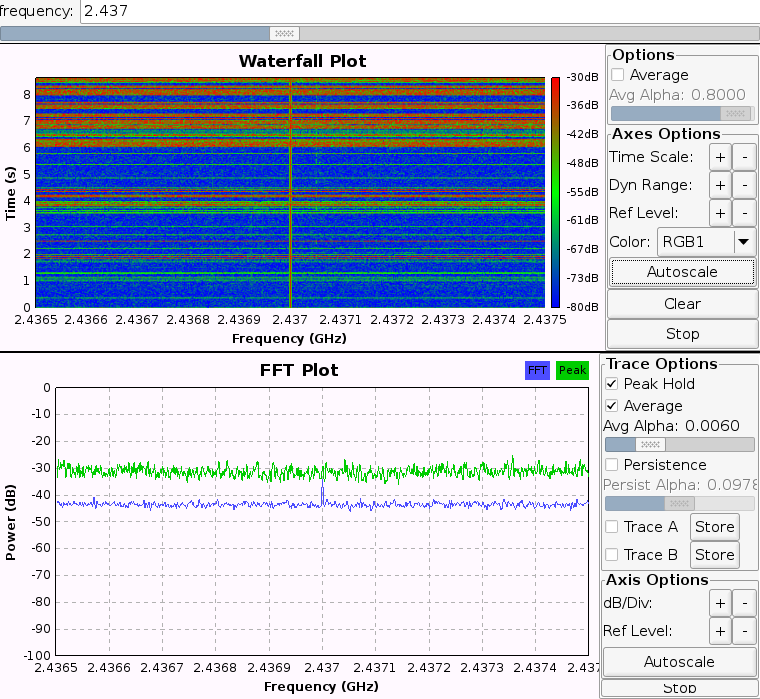
\includegraphics[width=0.9\textwidth]{figures/ch6.png}
\label{spectrum2437}
\caption{RF-Spectrum on \SI{2.437}{\giga\hertz}}
\end{figure}

\begin{figure}[H]
	\centering
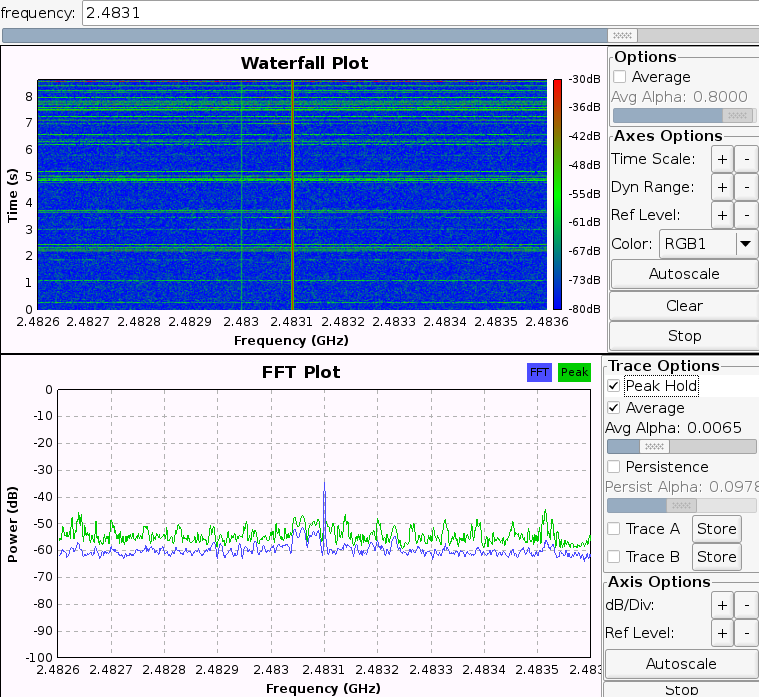
\includegraphics[width=0.9\textwidth]{figures/ranging_0.png}
\label{spectrum2483}
\caption{RF-Spectrum on \SI{2.483}{\giga\hertz}}
\end{figure}


\subsection{Influence of DQF on Range Values}
One value the ranging api provides is the DQF\footnote{Data Quality Factor}-value.
It is reasonable to expect a huge amount of scatter for lower DQF values.
As \autoref{1m_scatterplot} shows this is not how the range value behaves.

For the values measured with \SI{1}{\metre} real distance we can see that the values measered with lower quality do not have the same mean value as those with higher quality.
Also values measured with lower quality are closer to each other than those with higher signal quality.
As long as we only look at the values taken at \SI{1}{\metre} real distance it seams like we could be able to improve the range estimate by including the dqf value into the computation of the distance.
To do that this behaviour would need to be stable accross different distances, i.e. no matter if the measurement is taken at \SI{1}{\metre} or \SI{3}{\metre} distance the when the dqf is low the measured range is lower and if dqf is high the measured range is higher.
\begin{figure}[H]
	\centering
	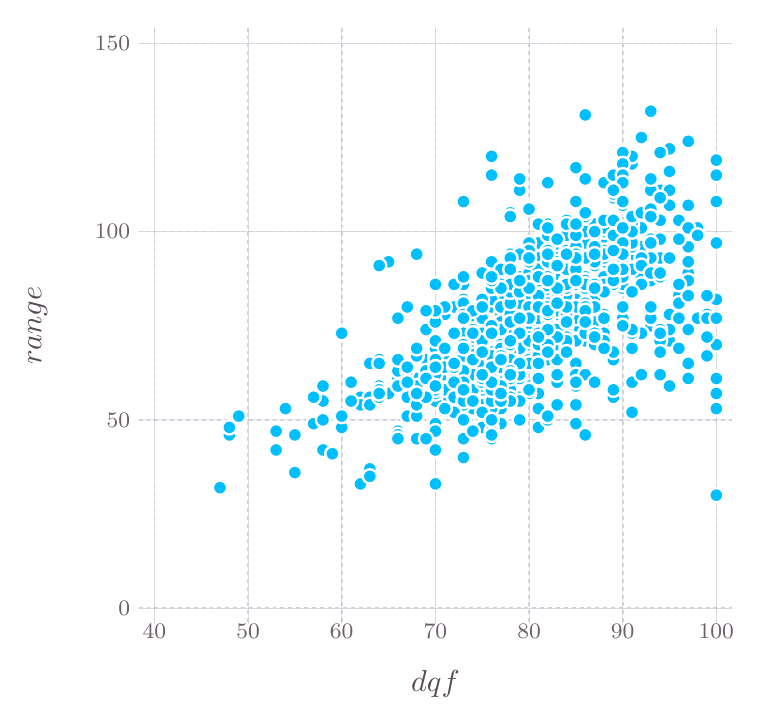
\begin{tikzpicture}[x=1mm,y=-1mm]
\definecolor{mycolor00BFFF}{rgb}{0,0.75,1}
\definecolor{mycolor564A55}{rgb}{0.34,0.29,0.33}
\definecolor{mycolor000000}{rgb}{0,0,0}
\definecolor{mycolor6C606B}{rgb}{0.42,0.38,0.42}
\definecolor{mycolorD0D0E0}{rgb}{0.82,0.82,0.88}
\definecolor{mycolorFFFFFF}{rgb}{1,1,1}
\definecolor{mycolor000000}{rgb}{0,0,0}
\begin{scope}
\begin{scope}
\draw (57.32,88.39) node [text=mycolor564A55,draw=mycolor000000,draw opacity=0,rotate around={-0: (0,1.81)},inner sep=0.0]{\fontsize{3.88mm}{4.66mm}\selectfont $\text{dqf}$};
\end{scope}
\begin{scope}
\draw (21.63,81.72) node [text=mycolor6C606B,rotate around={-0: (35.68,1.34)},inner sep=0.0]{\fontsize{2.82mm}{3.39mm}\selectfont $\text{40}$};
\draw (33.53,81.72) node [text=mycolor6C606B,rotate around={-0: (23.79,1.34)},inner sep=0.0]{\fontsize{2.82mm}{3.39mm}\selectfont $\text{50}$};
\draw (45.42,81.72) node [text=mycolor6C606B,rotate around={-0: (11.89,1.34)},inner sep=0.0]{\fontsize{2.82mm}{3.39mm}\selectfont $\text{60}$};
\draw (57.32,81.72) node [text=mycolor6C606B,rotate around={-0: (-0,1.34)},inner sep=0.0]{\fontsize{2.82mm}{3.39mm}\selectfont $\text{70}$};
\draw (69.21,81.72) node [text=mycolor6C606B,rotate around={-0: (-11.89,1.34)},inner sep=0.0]{\fontsize{2.82mm}{3.39mm}\selectfont $\text{80}$};
\draw (81.11,81.72) node [text=mycolor6C606B,rotate around={-0: (-23.79,1.34)},inner sep=0.0]{\fontsize{2.82mm}{3.39mm}\selectfont $\text{90}$};
\draw (93,81.72) node [text=mycolor6C606B,rotate around={-0: (-35.68,1.34)},inner sep=0.0]{\fontsize{2.82mm}{3.39mm}\selectfont $\text{100}$};
\end{scope}
\begin{scope}
\clip  (19.63,5) -- (95,5) -- (95,80.72) -- (19.63,80.72);
\begin{scope}
\clip  (19.63,5) -- (95,5) -- (95,80.72) -- (19.63,80.72);
\path [fill=mycolor000000,fill opacity=0,draw=mycolor000000,draw opacity=0] (19.63,5) rectangle +(75.37,75.72);
\end{scope}
\begin{scope}
[dash pattern=on 0.5mm off 0.5mm,line width=0.2mm]
\path [fill=mycolor000000,draw=mycolorD0D0E0]  (19.63,78.71) -- (95,78.71);
\path [fill=mycolor000000,draw=mycolorD0D0E0]  (19.63,54.81) -- (95,54.81);
\path [fill=mycolor000000,draw=mycolorD0D0E0]  (19.63,30.9) -- (95,30.9);
\path [fill=mycolor000000,draw=mycolorD0D0E0]  (19.63,7) -- (95,7);
\end{scope}
\begin{scope}
[dash pattern=on 0.5mm off 0.5mm,line width=0.2mm]
\path [fill=mycolor000000,draw=mycolorD0D0E0]  (21.63,5) -- (21.63,80.72);
\path [fill=mycolor000000,draw=mycolorD0D0E0]  (33.53,5) -- (33.53,80.72);
\path [fill=mycolor000000,draw=mycolorD0D0E0]  (45.42,5) -- (45.42,80.72);
\path [fill=mycolor000000,draw=mycolorD0D0E0]  (57.32,5) -- (57.32,80.72);
\path [fill=mycolor000000,draw=mycolorD0D0E0]  (69.21,5) -- (69.21,80.72);
\path [fill=mycolor000000,draw=mycolorD0D0E0]  (81.11,5) -- (81.11,80.72);
\path [fill=mycolor000000,draw=mycolorD0D0E0]  (93,5) -- (93,80.72);
\end{scope}
\begin{scope}
\begin{scope}
\begin{scope}
[line width=0.3mm]
\path [fill=mycolor00BFFF,draw=mycolorFFFFFF] (66.83,28.51) circle [radius=0.9];
\path [fill=mycolor00BFFF,draw=mycolorFFFFFF] (84.67,42.86) circle [radius=0.9];
\path [fill=mycolor00BFFF,draw=mycolorFFFFFF] (50.18,47.16) circle [radius=0.9];
\path [fill=mycolor00BFFF,draw=mycolorFFFFFF] (88.24,39.03) circle [radius=0.9];
\path [fill=mycolor00BFFF,draw=mycolorFFFFFF] (87.05,43.34) circle [radius=0.9];
\path [fill=mycolor00BFFF,draw=mycolorFFFFFF] (57.32,56.24) circle [radius=0.9];
\path [fill=mycolor00BFFF,draw=mycolorFFFFFF] (71.59,40.95) circle [radius=0.9];
\path [fill=mycolor00BFFF,draw=mycolorFFFFFF] (78.73,38.55) circle [radius=0.9];
\path [fill=mycolor00BFFF,draw=mycolorFFFFFF] (72.78,41.42) circle [radius=0.9];
\path [fill=mycolor00BFFF,draw=mycolorFFFFFF] (69.21,43.81) circle [radius=0.9];
\path [fill=mycolor00BFFF,draw=mycolorFFFFFF] (73.97,39.03) circle [radius=0.9];
\path [fill=mycolor00BFFF,draw=mycolorFFFFFF] (77.54,41.9) circle [radius=0.9];
\path [fill=mycolor00BFFF,draw=mycolorFFFFFF] (52.56,49.07) circle [radius=0.9];
\path [fill=mycolor00BFFF,draw=mycolorFFFFFF] (76.35,36.64) circle [radius=0.9];
\path [fill=mycolor00BFFF,draw=mycolorFFFFFF] (63.26,51.46) circle [radius=0.9];
\path [fill=mycolor00BFFF,draw=mycolorFFFFFF] (62.07,46.68) circle [radius=0.9];
\path [fill=mycolor00BFFF,draw=mycolorFFFFFF] (70.4,45.25) circle [radius=0.9];
\path [fill=mycolor00BFFF,draw=mycolorFFFFFF] (60.88,50.99) circle [radius=0.9];
\path [fill=mycolor00BFFF,draw=mycolorFFFFFF] (66.83,47.16) circle [radius=0.9];
\path [fill=mycolor00BFFF,draw=mycolorFFFFFF] (76.35,44.77) circle [radius=0.9];
\path [fill=mycolor00BFFF,draw=mycolorFFFFFF] (87.05,44.77) circle [radius=0.9];
\path [fill=mycolor00BFFF,draw=mycolorFFFFFF] (58.51,52.42) circle [radius=0.9];
\path [fill=mycolor00BFFF,draw=mycolorFFFFFF] (63.26,50.51) circle [radius=0.9];
\path [fill=mycolor00BFFF,draw=mycolorFFFFFF] (87.05,43.34) circle [radius=0.9];
\path [fill=mycolor00BFFF,draw=mycolorFFFFFF] (66.83,46.68) circle [radius=0.9];
\path [fill=mycolor00BFFF,draw=mycolorFFFFFF] (93,32.34) circle [radius=0.9];
\path [fill=mycolor00BFFF,draw=mycolorFFFFFF] (57.32,55.29) circle [radius=0.9];
\path [fill=mycolor00BFFF,draw=mycolorFFFFFF] (64.45,57.2) circle [radius=0.9];
\path [fill=mycolor00BFFF,draw=mycolorFFFFFF] (78.73,42.38) circle [radius=0.9];
\path [fill=mycolor00BFFF,draw=mycolorFFFFFF] (87.05,27.56) circle [radius=0.9];
\path [fill=mycolor00BFFF,draw=mycolorFFFFFF] (82.29,22.3) circle [radius=0.9];
\path [fill=mycolor00BFFF,draw=mycolorFFFFFF] (82.29,34.25) circle [radius=0.9];
\path [fill=mycolor00BFFF,draw=mycolorFFFFFF] (71.59,39.03) circle [radius=0.9];
\path [fill=mycolor00BFFF,draw=mycolorFFFFFF] (64.45,38.08) circle [radius=0.9];
\path [fill=mycolor00BFFF,draw=mycolorFFFFFF] (78.73,31.86) circle [radius=0.9];
\path [fill=mycolor00BFFF,draw=mycolorFFFFFF] (60.88,49.55) circle [radius=0.9];
\path [fill=mycolor00BFFF,draw=mycolorFFFFFF] (71.59,35.69) circle [radius=0.9];
\path [fill=mycolor00BFFF,draw=mycolorFFFFFF] (89.43,43.34) circle [radius=0.9];
\path [fill=mycolor00BFFF,draw=mycolorFFFFFF] (63.26,52.42) circle [radius=0.9];
\path [fill=mycolor00BFFF,draw=mycolorFFFFFF] (91.81,46.68) circle [radius=0.9];
\path [fill=mycolor00BFFF,draw=mycolorFFFFFF] (75.16,42.86) circle [radius=0.9];
\path [fill=mycolor00BFFF,draw=mycolorFFFFFF] (70.4,39.51) circle [radius=0.9];
\path [fill=mycolor00BFFF,draw=mycolorFFFFFF] (76.35,33.77) circle [radius=0.9];
\path [fill=mycolor00BFFF,draw=mycolorFFFFFF] (66.83,49.07) circle [radius=0.9];
\path [fill=mycolor00BFFF,draw=mycolorFFFFFF] (53.75,50.99) circle [radius=0.9];
\path [fill=mycolor00BFFF,draw=mycolorFFFFFF] (93,64.37) circle [radius=0.9];
\path [fill=mycolor00BFFF,draw=mycolorFFFFFF] (66.83,33.77) circle [radius=0.9];
\path [fill=mycolor00BFFF,draw=mycolorFFFFFF] (68.02,51.94) circle [radius=0.9];
\path [fill=mycolor00BFFF,draw=mycolorFFFFFF] (69.21,47.64) circle [radius=0.9];
\path [fill=mycolor00BFFF,draw=mycolorFFFFFF] (39.47,61.5) circle [radius=0.9];
\path [fill=mycolor00BFFF,draw=mycolorFFFFFF] (54.94,57.2) circle [radius=0.9];
\path [fill=mycolor00BFFF,draw=mycolorFFFFFF] (69.21,50.51) circle [radius=0.9];
\path [fill=mycolor00BFFF,draw=mycolorFFFFFF] (43.04,58.63) circle [radius=0.9];
\path [fill=mycolor00BFFF,draw=mycolorFFFFFF] (83.48,43.81) circle [radius=0.9];
\path [fill=mycolor00BFFF,draw=mycolorFFFFFF] (68.02,41.9) circle [radius=0.9];
\path [fill=mycolor00BFFF,draw=mycolorFFFFFF] (73.97,44.77) circle [radius=0.9];
\path [fill=mycolor00BFFF,draw=mycolorFFFFFF] (93,53.38) circle [radius=0.9];
\path [fill=mycolor00BFFF,draw=mycolorFFFFFF] (59.69,53.85) circle [radius=0.9];
\path [fill=mycolor00BFFF,draw=mycolorFFFFFF] (72.78,34.25) circle [radius=0.9];
\path [fill=mycolor00BFFF,draw=mycolorFFFFFF] (68.02,25.65) circle [radius=0.9];
\path [fill=mycolor00BFFF,draw=mycolorFFFFFF] (71.59,39.99) circle [radius=0.9];
\path [fill=mycolor00BFFF,draw=mycolorFFFFFF] (79.92,32.82) circle [radius=0.9];
\path [fill=mycolor00BFFF,draw=mycolorFFFFFF] (69.21,33.3) circle [radius=0.9];
\path [fill=mycolor00BFFF,draw=mycolorFFFFFF] (82.29,34.25) circle [radius=0.9];
\path [fill=mycolor00BFFF,draw=mycolorFFFFFF] (79.92,36.16) circle [radius=0.9];
\path [fill=mycolor00BFFF,draw=mycolorFFFFFF] (75.16,36.64) circle [radius=0.9];
\path [fill=mycolor00BFFF,draw=mycolorFFFFFF] (60.88,43.34) circle [radius=0.9];
\path [fill=mycolor00BFFF,draw=mycolorFFFFFF] (58.51,41.42) circle [radius=0.9];
\path [fill=mycolor00BFFF,draw=mycolorFFFFFF] (63.26,39.51) circle [radius=0.9];
\path [fill=mycolor00BFFF,draw=mycolorFFFFFF] (69.21,46.68) circle [radius=0.9];
\path [fill=mycolor00BFFF,draw=mycolorFFFFFF] (64.45,49.07) circle [radius=0.9];
\path [fill=mycolor00BFFF,draw=mycolorFFFFFF] (64.45,39.51) circle [radius=0.9];
\path [fill=mycolor00BFFF,draw=mycolorFFFFFF] (63.26,40.95) circle [radius=0.9];
\path [fill=mycolor00BFFF,draw=mycolorFFFFFF] (66.83,39.51) circle [radius=0.9];
\path [fill=mycolor00BFFF,draw=mycolorFFFFFF] (72.78,47.64) circle [radius=0.9];
\path [fill=mycolor00BFFF,draw=mycolorFFFFFF] (63.26,52.42) circle [radius=0.9];
\path [fill=mycolor00BFFF,draw=mycolorFFFFFF] (50.18,50.51) circle [radius=0.9];
\path [fill=mycolor00BFFF,draw=mycolorFFFFFF] (64.45,50.03) circle [radius=0.9];
\path [fill=mycolor00BFFF,draw=mycolorFFFFFF] (82.29,21.34) circle [radius=0.9];
\path [fill=mycolor00BFFF,draw=mycolorFFFFFF] (72.78,44.77) circle [radius=0.9];
\path [fill=mycolor00BFFF,draw=mycolorFFFFFF] (63.26,43.34) circle [radius=0.9];
\path [fill=mycolor00BFFF,draw=mycolorFFFFFF] (68.02,45.73) circle [radius=0.9];
\path [fill=mycolor00BFFF,draw=mycolorFFFFFF] (51.37,34.73) circle [radius=0.9];
\path [fill=mycolor00BFFF,draw=mycolorFFFFFF] (68.02,24.21) circle [radius=0.9];
\path [fill=mycolor00BFFF,draw=mycolorFFFFFF] (54.94,46.68) circle [radius=0.9];
\path [fill=mycolor00BFFF,draw=mycolorFFFFFF] (82.29,53.85) circle [radius=0.9];
\path [fill=mycolor00BFFF,draw=mycolorFFFFFF] (62.07,48.59) circle [radius=0.9];
\path [fill=mycolor00BFFF,draw=mycolorFFFFFF] (68.02,37.6) circle [radius=0.9];
\path [fill=mycolor00BFFF,draw=mycolorFFFFFF] (75.16,35.21) circle [radius=0.9];
\path [fill=mycolor00BFFF,draw=mycolorFFFFFF] (68.02,43.81) circle [radius=0.9];
\path [fill=mycolor00BFFF,draw=mycolorFFFFFF] (63.26,49.55) circle [radius=0.9];
\path [fill=mycolor00BFFF,draw=mycolorFFFFFF] (70.4,34.25) circle [radius=0.9];
\path [fill=mycolor00BFFF,draw=mycolorFFFFFF] (88.24,45.73) circle [radius=0.9];
\path [fill=mycolor00BFFF,draw=mycolorFFFFFF] (56.13,49.07) circle [radius=0.9];
\path [fill=mycolor00BFFF,draw=mycolorFFFFFF] (75.16,36.64) circle [radius=0.9];
\path [fill=mycolor00BFFF,draw=mycolorFFFFFF] (62.07,52.9) circle [radius=0.9];
\path [fill=mycolor00BFFF,draw=mycolorFFFFFF] (75.16,32.82) circle [radius=0.9];
\path [fill=mycolor00BFFF,draw=mycolorFFFFFF] (78.73,30.9) circle [radius=0.9];
\path [fill=mycolor00BFFF,draw=mycolorFFFFFF] (73.97,42.86) circle [radius=0.9];
\path [fill=mycolor00BFFF,draw=mycolorFFFFFF] (58.51,49.07) circle [radius=0.9];
\path [fill=mycolor00BFFF,draw=mycolorFFFFFF] (89.43,27.56) circle [radius=0.9];
\path [fill=mycolor00BFFF,draw=mycolorFFFFFF] (62.07,41.9) circle [radius=0.9];
\path [fill=mycolor00BFFF,draw=mycolorFFFFFF] (73.97,40.95) circle [radius=0.9];
\path [fill=mycolor00BFFF,draw=mycolorFFFFFF] (75.16,36.16) circle [radius=0.9];
\path [fill=mycolor00BFFF,draw=mycolorFFFFFF] (78.73,36.64) circle [radius=0.9];
\path [fill=mycolor00BFFF,draw=mycolorFFFFFF] (71.59,29.95) circle [radius=0.9];
\path [fill=mycolor00BFFF,draw=mycolorFFFFFF] (72.78,47.64) circle [radius=0.9];
\path [fill=mycolor00BFFF,draw=mycolorFFFFFF] (70.4,51.46) circle [radius=0.9];
\path [fill=mycolor00BFFF,draw=mycolorFFFFFF] (79.92,37.12) circle [radius=0.9];
\path [fill=mycolor00BFFF,draw=mycolorFFFFFF] (85.86,43.34) circle [radius=0.9];
\path [fill=mycolor00BFFF,draw=mycolorFFFFFF] (56.13,49.55) circle [radius=0.9];
\path [fill=mycolor00BFFF,draw=mycolorFFFFFF] (59.69,50.99) circle [radius=0.9];
\path [fill=mycolor00BFFF,draw=mycolorFFFFFF] (85.86,25.65) circle [radius=0.9];
\path [fill=mycolor00BFFF,draw=mycolorFFFFFF] (52.56,49.55) circle [radius=0.9];
\path [fill=mycolor00BFFF,draw=mycolorFFFFFF] (77.54,40.95) circle [radius=0.9];
\path [fill=mycolor00BFFF,draw=mycolorFFFFFF] (66.83,48.12) circle [radius=0.9];
\path [fill=mycolor00BFFF,draw=mycolorFFFFFF] (77.54,39.03) circle [radius=0.9];
\path [fill=mycolor00BFFF,draw=mycolorFFFFFF] (77.54,42.38) circle [radius=0.9];
\path [fill=mycolor00BFFF,draw=mycolorFFFFFF] (65.64,43.34) circle [radius=0.9];
\path [fill=mycolor00BFFF,draw=mycolorFFFFFF] (60.88,43.34) circle [radius=0.9];
\path [fill=mycolor00BFFF,draw=mycolorFFFFFF] (68.02,36.64) circle [radius=0.9];
\path [fill=mycolor00BFFF,draw=mycolorFFFFFF] (72.78,35.21) circle [radius=0.9];
\path [fill=mycolor00BFFF,draw=mycolorFFFFFF] (53.75,49.55) circle [radius=0.9];
\path [fill=mycolor00BFFF,draw=mycolorFFFFFF] (66.83,36.16) circle [radius=0.9];
\path [fill=mycolor00BFFF,draw=mycolorFFFFFF] (78.73,37.6) circle [radius=0.9];
\path [fill=mycolor00BFFF,draw=mycolorFFFFFF] (71.59,43.81) circle [radius=0.9];
\path [fill=mycolor00BFFF,draw=mycolorFFFFFF] (72.78,43.81) circle [radius=0.9];
\path [fill=mycolor00BFFF,draw=mycolorFFFFFF] (66.83,28.99) circle [radius=0.9];
\path [fill=mycolor00BFFF,draw=mycolorFFFFFF] (66.83,49.07) circle [radius=0.9];
\path [fill=mycolor00BFFF,draw=mycolorFFFFFF] (76.35,41.42) circle [radius=0.9];
\path [fill=mycolor00BFFF,draw=mycolorFFFFFF] (71.59,41.42) circle [radius=0.9];
\path [fill=mycolor00BFFF,draw=mycolorFFFFFF] (76.35,41.9) circle [radius=0.9];
\path [fill=mycolor00BFFF,draw=mycolorFFFFFF] (50.18,35.21) circle [radius=0.9];
\path [fill=mycolor00BFFF,draw=mycolorFFFFFF] (48.99,47.64) circle [radius=0.9];
\path [fill=mycolor00BFFF,draw=mycolorFFFFFF] (85.86,34.25) circle [radius=0.9];
\path [fill=mycolor00BFFF,draw=mycolorFFFFFF] (58.51,41.42) circle [radius=0.9];
\path [fill=mycolor00BFFF,draw=mycolorFFFFFF] (65.64,38.08) circle [radius=0.9];
\path [fill=mycolor00BFFF,draw=mycolorFFFFFF] (52.56,48.59) circle [radius=0.9];
\path [fill=mycolor00BFFF,draw=mycolorFFFFFF] (70.4,49.55) circle [radius=0.9];
\path [fill=mycolor00BFFF,draw=mycolorFFFFFF] (71.59,44.29) circle [radius=0.9];
\path [fill=mycolor00BFFF,draw=mycolorFFFFFF] (71.59,43.34) circle [radius=0.9];
\path [fill=mycolor00BFFF,draw=mycolorFFFFFF] (63.26,50.99) circle [radius=0.9];
\path [fill=mycolor00BFFF,draw=mycolorFFFFFF] (63.26,40.47) circle [radius=0.9];
\path [fill=mycolor00BFFF,draw=mycolorFFFFFF] (76.35,43.81) circle [radius=0.9];
\path [fill=mycolor00BFFF,draw=mycolorFFFFFF] (78.73,34.73) circle [radius=0.9];
\path [fill=mycolor00BFFF,draw=mycolorFFFFFF] (88.24,29.47) circle [radius=0.9];
\path [fill=mycolor00BFFF,draw=mycolorFFFFFF] (52.56,47.16) circle [radius=0.9];
\path [fill=mycolor00BFFF,draw=mycolorFFFFFF] (70.4,33.3) circle [radius=0.9];
\path [fill=mycolor00BFFF,draw=mycolorFFFFFF] (69.21,28.04) circle [radius=0.9];
\path [fill=mycolor00BFFF,draw=mycolorFFFFFF] (71.59,47.16) circle [radius=0.9];
\path [fill=mycolor00BFFF,draw=mycolorFFFFFF] (66.83,45.25) circle [radius=0.9];
\path [fill=mycolor00BFFF,draw=mycolorFFFFFF] (81.11,20.86) circle [radius=0.9];
\path [fill=mycolor00BFFF,draw=mycolorFFFFFF] (72.78,33.3) circle [radius=0.9];
\path [fill=mycolor00BFFF,draw=mycolorFFFFFF] (72.78,39.99) circle [radius=0.9];
\path [fill=mycolor00BFFF,draw=mycolorFFFFFF] (71.59,40.47) circle [radius=0.9];
\path [fill=mycolor00BFFF,draw=mycolorFFFFFF] (76.35,29.47) circle [radius=0.9];
\path [fill=mycolor00BFFF,draw=mycolorFFFFFF] (73.97,35.69) circle [radius=0.9];
\path [fill=mycolor00BFFF,draw=mycolorFFFFFF] (70.4,32.34) circle [radius=0.9];
\path [fill=mycolor00BFFF,draw=mycolorFFFFFF] (72.78,39.03) circle [radius=0.9];
\path [fill=mycolor00BFFF,draw=mycolorFFFFFF] (63.26,42.38) circle [radius=0.9];
\path [fill=mycolor00BFFF,draw=mycolorFFFFFF] (54.94,33.77) circle [radius=0.9];
\path [fill=mycolor00BFFF,draw=mycolorFFFFFF] (59.69,49.07) circle [radius=0.9];
\path [fill=mycolor00BFFF,draw=mycolorFFFFFF] (70.4,34.25) circle [radius=0.9];
\path [fill=mycolor00BFFF,draw=mycolorFFFFFF] (56.13,43.34) circle [radius=0.9];
\path [fill=mycolor00BFFF,draw=mycolorFFFFFF] (73.97,37.12) circle [radius=0.9];
\path [fill=mycolor00BFFF,draw=mycolorFFFFFF] (73.97,41.42) circle [radius=0.9];
\path [fill=mycolor00BFFF,draw=mycolorFFFFFF] (59.69,49.07) circle [radius=0.9];
\path [fill=mycolor00BFFF,draw=mycolorFFFFFF] (77.54,30.43) circle [radius=0.9];
\path [fill=mycolor00BFFF,draw=mycolorFFFFFF] (68.02,39.51) circle [radius=0.9];
\path [fill=mycolor00BFFF,draw=mycolorFFFFFF] (60.88,37.12) circle [radius=0.9];
\path [fill=mycolor00BFFF,draw=mycolorFFFFFF] (83.48,35.69) circle [radius=0.9];
\path [fill=mycolor00BFFF,draw=mycolorFFFFFF] (65.64,55.29) circle [radius=0.9];
\path [fill=mycolor00BFFF,draw=mycolorFFFFFF] (47.8,62.94) circle [radius=0.9];
\path [fill=mycolor00BFFF,draw=mycolorFFFFFF] (83.48,32.82) circle [radius=0.9];
\path [fill=mycolor00BFFF,draw=mycolorFFFFFF] (65.64,39.51) circle [radius=0.9];
\path [fill=mycolor00BFFF,draw=mycolorFFFFFF] (69.21,36.16) circle [radius=0.9];
\path [fill=mycolor00BFFF,draw=mycolorFFFFFF] (82.29,32.82) circle [radius=0.9];
\path [fill=mycolor00BFFF,draw=mycolorFFFFFF] (85.86,44.77) circle [radius=0.9];
\path [fill=mycolor00BFFF,draw=mycolorFFFFFF] (45.42,55.77) circle [radius=0.9];
\path [fill=mycolor00BFFF,draw=mycolorFFFFFF] (71.59,40.47) circle [radius=0.9];
\path [fill=mycolor00BFFF,draw=mycolorFFFFFF] (93,39.51) circle [radius=0.9];
\path [fill=mycolor00BFFF,draw=mycolorFFFFFF] (57.32,45.73) circle [radius=0.9];
\path [fill=mycolor00BFFF,draw=mycolorFFFFFF] (66.83,50.99) circle [radius=0.9];
\path [fill=mycolor00BFFF,draw=mycolorFFFFFF] (60.88,47.64) circle [radius=0.9];
\path [fill=mycolor00BFFF,draw=mycolorFFFFFF] (77.54,50.03) circle [radius=0.9];
\path [fill=mycolor00BFFF,draw=mycolorFFFFFF] (60.88,52.42) circle [radius=0.9];
\path [fill=mycolor00BFFF,draw=mycolorFFFFFF] (82.29,30.9) circle [radius=0.9];
\path [fill=mycolor00BFFF,draw=mycolorFFFFFF] (72.78,31.86) circle [radius=0.9];
\path [fill=mycolor00BFFF,draw=mycolorFFFFFF] (64.45,23.73) circle [radius=0.9];
\path [fill=mycolor00BFFF,draw=mycolorFFFFFF] (70.4,29.95) circle [radius=0.9];
\path [fill=mycolor00BFFF,draw=mycolorFFFFFF] (62.07,50.99) circle [radius=0.9];
\path [fill=mycolor00BFFF,draw=mycolorFFFFFF] (85.86,43.81) circle [radius=0.9];
\path [fill=mycolor00BFFF,draw=mycolorFFFFFF] (38.28,53.38) circle [radius=0.9];
\path [fill=mycolor00BFFF,draw=mycolorFFFFFF] (81.11,35.69) circle [radius=0.9];
\path [fill=mycolor00BFFF,draw=mycolorFFFFFF] (77.54,39.03) circle [radius=0.9];
\path [fill=mycolor00BFFF,draw=mycolorFFFFFF] (69.21,42.86) circle [radius=0.9];
\path [fill=mycolor00BFFF,draw=mycolorFFFFFF] (53.75,54.33) circle [radius=0.9];
\path [fill=mycolor00BFFF,draw=mycolorFFFFFF] (81.11,40.47) circle [radius=0.9];
\path [fill=mycolor00BFFF,draw=mycolorFFFFFF] (90.62,30.43) circle [radius=0.9];
\path [fill=mycolor00BFFF,draw=mycolorFFFFFF] (93,21.82) circle [radius=0.9];
\path [fill=mycolor00BFFF,draw=mycolorFFFFFF] (58.51,41.42) circle [radius=0.9];
\path [fill=mycolor00BFFF,draw=mycolorFFFFFF] (62.07,45.25) circle [radius=0.9];
\path [fill=mycolor00BFFF,draw=mycolorFFFFFF] (76.35,24.21) circle [radius=0.9];
\path [fill=mycolor00BFFF,draw=mycolorFFFFFF] (64.45,47.64) circle [radius=0.9];
\path [fill=mycolor00BFFF,draw=mycolorFFFFFF] (69.21,37.12) circle [radius=0.9];
\path [fill=mycolor00BFFF,draw=mycolorFFFFFF] (71.59,42.38) circle [radius=0.9];
\path [fill=mycolor00BFFF,draw=mycolorFFFFFF] (66.83,43.34) circle [radius=0.9];
\path [fill=mycolor00BFFF,draw=mycolorFFFFFF] (57.32,50.99) circle [radius=0.9];
\path [fill=mycolor00BFFF,draw=mycolorFFFFFF] (72.78,36.64) circle [radius=0.9];
\path [fill=mycolor00BFFF,draw=mycolorFFFFFF] (70.4,46.68) circle [radius=0.9];
\path [fill=mycolor00BFFF,draw=mycolorFFFFFF] (81.11,34.73) circle [radius=0.9];
\path [fill=mycolor00BFFF,draw=mycolorFFFFFF] (77.54,38.08) circle [radius=0.9];
\path [fill=mycolor00BFFF,draw=mycolorFFFFFF] (82.29,31.38) circle [radius=0.9];
\path [fill=mycolor00BFFF,draw=mycolorFFFFFF] (79.92,33.3) circle [radius=0.9];
\path [fill=mycolor00BFFF,draw=mycolorFFFFFF] (76.35,38.08) circle [radius=0.9];
\path [fill=mycolor00BFFF,draw=mycolorFFFFFF] (69.21,41.9) circle [radius=0.9];
\path [fill=mycolor00BFFF,draw=mycolorFFFFFF] (83.48,34.73) circle [radius=0.9];
\path [fill=mycolor00BFFF,draw=mycolorFFFFFF] (84.67,31.86) circle [radius=0.9];
\path [fill=mycolor00BFFF,draw=mycolorFFFFFF] (77.54,45.25) circle [radius=0.9];
\path [fill=mycolor00BFFF,draw=mycolorFFFFFF] (81.11,38.08) circle [radius=0.9];
\path [fill=mycolor00BFFF,draw=mycolorFFFFFF] (72.78,44.29) circle [radius=0.9];
\path [fill=mycolor00BFFF,draw=mycolorFFFFFF] (84.67,32.34) circle [radius=0.9];
\path [fill=mycolor00BFFF,draw=mycolorFFFFFF] (65.64,43.81) circle [radius=0.9];
\path [fill=mycolor00BFFF,draw=mycolorFFFFFF] (77.54,31.38) circle [radius=0.9];
\path [fill=mycolor00BFFF,draw=mycolorFFFFFF] (89.43,30.43) circle [radius=0.9];
\path [fill=mycolor00BFFF,draw=mycolorFFFFFF] (82.29,33.77) circle [radius=0.9];
\path [fill=mycolor00BFFF,draw=mycolorFFFFFF] (84.67,37.12) circle [radius=0.9];
\path [fill=mycolor00BFFF,draw=mycolorFFFFFF] (83.48,30.43) circle [radius=0.9];
\path [fill=mycolor00BFFF,draw=mycolorFFFFFF] (81.11,37.6) circle [radius=0.9];
\path [fill=mycolor00BFFF,draw=mycolorFFFFFF] (84.67,31.86) circle [radius=0.9];
\path [fill=mycolor00BFFF,draw=mycolorFFFFFF] (82.29,29.47) circle [radius=0.9];
\path [fill=mycolor00BFFF,draw=mycolorFFFFFF] (78.73,24.69) circle [radius=0.9];
\path [fill=mycolor00BFFF,draw=mycolorFFFFFF] (65.64,52.42) circle [radius=0.9];
\path [fill=mycolor00BFFF,draw=mycolorFFFFFF] (54.94,51.46) circle [radius=0.9];
\path [fill=mycolor00BFFF,draw=mycolorFFFFFF] (68.02,44.77) circle [radius=0.9];
\path [fill=mycolor00BFFF,draw=mycolorFFFFFF] (77.54,35.21) circle [radius=0.9];
\path [fill=mycolor00BFFF,draw=mycolorFFFFFF] (70.4,43.34) circle [radius=0.9];
\path [fill=mycolor00BFFF,draw=mycolorFFFFFF] (84.67,34.25) circle [radius=0.9];
\path [fill=mycolor00BFFF,draw=mycolorFFFFFF] (83.48,36.64) circle [radius=0.9];
\path [fill=mycolor00BFFF,draw=mycolorFFFFFF] (76.35,38.55) circle [radius=0.9];
\path [fill=mycolor00BFFF,draw=mycolorFFFFFF] (65.64,46.68) circle [radius=0.9];
\path [fill=mycolor00BFFF,draw=mycolorFFFFFF] (76.35,41.9) circle [radius=0.9];
\path [fill=mycolor00BFFF,draw=mycolorFFFFFF] (77.54,39.03) circle [radius=0.9];
\path [fill=mycolor00BFFF,draw=mycolorFFFFFF] (82.29,35.69) circle [radius=0.9];
\path [fill=mycolor00BFFF,draw=mycolorFFFFFF] (84.67,28.51) circle [radius=0.9];
\path [fill=mycolor00BFFF,draw=mycolorFFFFFF] (76.35,40.47) circle [radius=0.9];
\path [fill=mycolor00BFFF,draw=mycolorFFFFFF] (68.02,39.03) circle [radius=0.9];
\path [fill=mycolor00BFFF,draw=mycolorFFFFFF] (64.45,50.03) circle [radius=0.9];
\path [fill=mycolor00BFFF,draw=mycolorFFFFFF] (72.78,39.51) circle [radius=0.9];
\path [fill=mycolor00BFFF,draw=mycolorFFFFFF] (69.21,47.16) circle [radius=0.9];
\path [fill=mycolor00BFFF,draw=mycolorFFFFFF] (73.97,43.81) circle [radius=0.9];
\path [fill=mycolor00BFFF,draw=mycolorFFFFFF] (73.97,44.29) circle [radius=0.9];
\path [fill=mycolor00BFFF,draw=mycolorFFFFFF] (69.21,42.86) circle [radius=0.9];
\path [fill=mycolor00BFFF,draw=mycolorFFFFFF] (83.48,34.25) circle [radius=0.9];
\path [fill=mycolor00BFFF,draw=mycolorFFFFFF] (48.99,61.5) circle [radius=0.9];
\path [fill=mycolor00BFFF,draw=mycolorFFFFFF] (48.99,61.5) circle [radius=0.9];
\path [fill=mycolor00BFFF,draw=mycolorFFFFFF] (73.97,35.21) circle [radius=0.9];
\path [fill=mycolor00BFFF,draw=mycolorFFFFFF] (82.29,29.95) circle [radius=0.9];
\path [fill=mycolor00BFFF,draw=mycolorFFFFFF] (78.73,41.42) circle [radius=0.9];
\path [fill=mycolor00BFFF,draw=mycolorFFFFFF] (66.83,49.07) circle [radius=0.9];
\path [fill=mycolor00BFFF,draw=mycolorFFFFFF] (75.16,41.42) circle [radius=0.9];
\path [fill=mycolor00BFFF,draw=mycolorFFFFFF] (58.51,47.16) circle [radius=0.9];
\path [fill=mycolor00BFFF,draw=mycolorFFFFFF] (59.69,40.47) circle [radius=0.9];
\path [fill=mycolor00BFFF,draw=mycolorFFFFFF] (32.34,54.33) circle [radius=0.9];
\path [fill=mycolor00BFFF,draw=mycolorFFFFFF] (75.16,38.08) circle [radius=0.9];
\path [fill=mycolor00BFFF,draw=mycolorFFFFFF] (57.32,56.24) circle [radius=0.9];
\path [fill=mycolor00BFFF,draw=mycolorFFFFFF] (31.15,56.72) circle [radius=0.9];
\path [fill=mycolor00BFFF,draw=mycolorFFFFFF] (81.11,30.43) circle [radius=0.9];
\path [fill=mycolor00BFFF,draw=mycolorFFFFFF] (65.64,50.51) circle [radius=0.9];
\path [fill=mycolor00BFFF,draw=mycolorFFFFFF] (75.16,44.77) circle [radius=0.9];
\path [fill=mycolor00BFFF,draw=mycolorFFFFFF] (69.21,51.46) circle [radius=0.9];
\path [fill=mycolor00BFFF,draw=mycolorFFFFFF] (77.54,38.08) circle [radius=0.9];
\path [fill=mycolor00BFFF,draw=mycolorFFFFFF] (78.73,37.6) circle [radius=0.9];
\path [fill=mycolor00BFFF,draw=mycolorFFFFFF] (76.35,37.12) circle [radius=0.9];
\path [fill=mycolor00BFFF,draw=mycolorFFFFFF] (57.32,52.42) circle [radius=0.9];
\path [fill=mycolor00BFFF,draw=mycolorFFFFFF] (76.35,41.42) circle [radius=0.9];
\path [fill=mycolor00BFFF,draw=mycolorFFFFFF] (78.73,34.25) circle [radius=0.9];
\path [fill=mycolor00BFFF,draw=mycolorFFFFFF] (43.04,50.51) circle [radius=0.9];
\path [fill=mycolor00BFFF,draw=mycolorFFFFFF] (63.26,53.38) circle [radius=0.9];
\path [fill=mycolor00BFFF,draw=mycolorFFFFFF] (77.54,34.73) circle [radius=0.9];
\path [fill=mycolor00BFFF,draw=mycolorFFFFFF] (65.64,48.59) circle [radius=0.9];
\path [fill=mycolor00BFFF,draw=mycolorFFFFFF] (69.21,45.25) circle [radius=0.9];
\path [fill=mycolor00BFFF,draw=mycolorFFFFFF] (68.02,44.77) circle [radius=0.9];
\path [fill=mycolor00BFFF,draw=mycolorFFFFFF] (75.16,39.51) circle [radius=0.9];
\path [fill=mycolor00BFFF,draw=mycolorFFFFFF] (70.4,41.42) circle [radius=0.9];
\path [fill=mycolor00BFFF,draw=mycolorFFFFFF] (79.92,37.6) circle [radius=0.9];
\path [fill=mycolor00BFFF,draw=mycolorFFFFFF] (93,23.73) circle [radius=0.9];
\path [fill=mycolor00BFFF,draw=mycolorFFFFFF] (77.54,35.21) circle [radius=0.9];
\path [fill=mycolor00BFFF,draw=mycolorFFFFFF] (66.83,43.81) circle [radius=0.9];
\path [fill=mycolor00BFFF,draw=mycolorFFFFFF] (84.67,25.65) circle [radius=0.9];
\path [fill=mycolor00BFFF,draw=mycolorFFFFFF] (85.86,31.86) circle [radius=0.9];
\path [fill=mycolor00BFFF,draw=mycolorFFFFFF] (76.35,37.12) circle [radius=0.9];
\path [fill=mycolor00BFFF,draw=mycolorFFFFFF] (78.73,38.55) circle [radius=0.9];
\path [fill=mycolor00BFFF,draw=mycolorFFFFFF] (85.86,36.64) circle [radius=0.9];
\path [fill=mycolor00BFFF,draw=mycolorFFFFFF] (78.73,37.6) circle [radius=0.9];
\path [fill=mycolor00BFFF,draw=mycolorFFFFFF] (73.97,37.12) circle [radius=0.9];
\path [fill=mycolor00BFFF,draw=mycolorFFFFFF] (82.29,32.82) circle [radius=0.9];
\path [fill=mycolor00BFFF,draw=mycolorFFFFFF] (70.4,44.29) circle [radius=0.9];
\path [fill=mycolor00BFFF,draw=mycolorFFFFFF] (70.4,45.73) circle [radius=0.9];
\path [fill=mycolor00BFFF,draw=mycolorFFFFFF] (64.45,47.16) circle [radius=0.9];
\path [fill=mycolor00BFFF,draw=mycolorFFFFFF] (66.83,46.68) circle [radius=0.9];
\path [fill=mycolor00BFFF,draw=mycolorFFFFFF] (59.69,52.9) circle [radius=0.9];
\path [fill=mycolor00BFFF,draw=mycolorFFFFFF] (65.64,50.99) circle [radius=0.9];
\path [fill=mycolor00BFFF,draw=mycolorFFFFFF] (44.23,59.11) circle [radius=0.9];
\path [fill=mycolor00BFFF,draw=mycolorFFFFFF] (44.23,59.11) circle [radius=0.9];
\path [fill=mycolor00BFFF,draw=mycolorFFFFFF] (70.4,49.07) circle [radius=0.9];
\path [fill=mycolor00BFFF,draw=mycolorFFFFFF] (77.54,45.25) circle [radius=0.9];
\path [fill=mycolor00BFFF,draw=mycolorFFFFFF] (66.83,42.86) circle [radius=0.9];
\path [fill=mycolor00BFFF,draw=mycolorFFFFFF] (64.45,50.51) circle [radius=0.9];
\path [fill=mycolor00BFFF,draw=mycolorFFFFFF] (63.26,41.9) circle [radius=0.9];
\path [fill=mycolor00BFFF,draw=mycolorFFFFFF] (68.02,49.55) circle [radius=0.9];
\path [fill=mycolor00BFFF,draw=mycolorFFFFFF] (65.64,53.38) circle [radius=0.9];
\path [fill=mycolor00BFFF,draw=mycolorFFFFFF] (60.88,59.59) circle [radius=0.9];
\path [fill=mycolor00BFFF,draw=mycolorFFFFFF] (65.64,51.46) circle [radius=0.9];
\path [fill=mycolor00BFFF,draw=mycolorFFFFFF] (70.4,45.25) circle [radius=0.9];
\path [fill=mycolor00BFFF,draw=mycolorFFFFFF] (60.88,57.2) circle [radius=0.9];
\path [fill=mycolor00BFFF,draw=mycolorFFFFFF] (64.45,57.2) circle [radius=0.9];
\path [fill=mycolor00BFFF,draw=mycolorFFFFFF] (70.4,55.77) circle [radius=0.9];
\path [fill=mycolor00BFFF,draw=mycolorFFFFFF] (65.64,50.03) circle [radius=0.9];
\path [fill=mycolor00BFFF,draw=mycolorFFFFFF] (48.99,61.03) circle [radius=0.9];
\path [fill=mycolor00BFFF,draw=mycolorFFFFFF] (57.32,58.63) circle [radius=0.9];
\path [fill=mycolor00BFFF,draw=mycolorFFFFFF] (73.97,39.03) circle [radius=0.9];
\path [fill=mycolor00BFFF,draw=mycolorFFFFFF] (75.16,52.9) circle [radius=0.9];
\path [fill=mycolor00BFFF,draw=mycolorFFFFFF] (62.07,50.99) circle [radius=0.9];
\path [fill=mycolor00BFFF,draw=mycolorFFFFFF] (78.73,43.81) circle [radius=0.9];
\path [fill=mycolor00BFFF,draw=mycolorFFFFFF] (77.54,33.3) circle [radius=0.9];
\path [fill=mycolor00BFFF,draw=mycolorFFFFFF] (77.54,39.51) circle [radius=0.9];
\path [fill=mycolor00BFFF,draw=mycolorFFFFFF] (69.21,34.25) circle [radius=0.9];
\path [fill=mycolor00BFFF,draw=mycolorFFFFFF] (73.97,39.51) circle [radius=0.9];
\path [fill=mycolor00BFFF,draw=mycolorFFFFFF] (60.88,50.99) circle [radius=0.9];
\path [fill=mycolor00BFFF,draw=mycolorFFFFFF] (64.45,55.77) circle [radius=0.9];
\path [fill=mycolor00BFFF,draw=mycolorFFFFFF] (64.45,46.2) circle [radius=0.9];
\path [fill=mycolor00BFFF,draw=mycolorFFFFFF] (64.45,53.38) circle [radius=0.9];
\path [fill=mycolor00BFFF,draw=mycolorFFFFFF] (76.35,56.72) circle [radius=0.9];
\path [fill=mycolor00BFFF,draw=mycolorFFFFFF] (64.45,43.34) circle [radius=0.9];
\path [fill=mycolor00BFFF,draw=mycolorFFFFFF] (68.02,42.38) circle [radius=0.9];
\path [fill=mycolor00BFFF,draw=mycolorFFFFFF] (46.61,50.03) circle [radius=0.9];
\path [fill=mycolor00BFFF,draw=mycolorFFFFFF] (66.83,44.77) circle [radius=0.9];
\path [fill=mycolor00BFFF,draw=mycolorFFFFFF] (68.02,37.6) circle [radius=0.9];
\path [fill=mycolor00BFFF,draw=mycolorFFFFFF] (63.26,46.68) circle [radius=0.9];
\path [fill=mycolor00BFFF,draw=mycolorFFFFFF] (63.26,50.99) circle [radius=0.9];
\path [fill=mycolor00BFFF,draw=mycolorFFFFFF] (63.26,55.77) circle [radius=0.9];
\path [fill=mycolor00BFFF,draw=mycolorFFFFFF] (62.07,51.46) circle [radius=0.9];
\path [fill=mycolor00BFFF,draw=mycolorFFFFFF] (63.26,52.9) circle [radius=0.9];
\path [fill=mycolor00BFFF,draw=mycolorFFFFFF] (57.32,46.68) circle [radius=0.9];
\path [fill=mycolor00BFFF,draw=mycolorFFFFFF] (70.4,46.2) circle [radius=0.9];
\path [fill=mycolor00BFFF,draw=mycolorFFFFFF] (66.83,47.64) circle [radius=0.9];
\path [fill=mycolor00BFFF,draw=mycolorFFFFFF] (71.59,38.55) circle [radius=0.9];
\path [fill=mycolor00BFFF,draw=mycolorFFFFFF] (63.26,50.51) circle [radius=0.9];
\path [fill=mycolor00BFFF,draw=mycolorFFFFFF] (47.8,51.94) circle [radius=0.9];
\path [fill=mycolor00BFFF,draw=mycolorFFFFFF] (66.83,44.77) circle [radius=0.9];
\path [fill=mycolor00BFFF,draw=mycolorFFFFFF] (75.16,41.9) circle [radius=0.9];
\path [fill=mycolor00BFFF,draw=mycolorFFFFFF] (73.97,31.38) circle [radius=0.9];
\path [fill=mycolor00BFFF,draw=mycolorFFFFFF] (66.83,49.07) circle [radius=0.9];
\path [fill=mycolor00BFFF,draw=mycolorFFFFFF] (60.88,39.51) circle [radius=0.9];
\path [fill=mycolor00BFFF,draw=mycolorFFFFFF] (64.45,47.16) circle [radius=0.9];
\path [fill=mycolor00BFFF,draw=mycolorFFFFFF] (71.59,42.38) circle [radius=0.9];
\path [fill=mycolor00BFFF,draw=mycolorFFFFFF] (62.07,50.99) circle [radius=0.9];
\path [fill=mycolor00BFFF,draw=mycolorFFFFFF] (70.4,43.81) circle [radius=0.9];
\path [fill=mycolor00BFFF,draw=mycolorFFFFFF] (69.21,39.99) circle [radius=0.9];
\path [fill=mycolor00BFFF,draw=mycolorFFFFFF] (78.73,33.3) circle [radius=0.9];
\path [fill=mycolor00BFFF,draw=mycolorFFFFFF] (51.37,51.46) circle [radius=0.9];
\path [fill=mycolor00BFFF,draw=mycolorFFFFFF] (72.78,39.03) circle [radius=0.9];
\path [fill=mycolor00BFFF,draw=mycolorFFFFFF] (73.97,39.51) circle [radius=0.9];
\path [fill=mycolor00BFFF,draw=mycolorFFFFFF] (63.26,46.2) circle [radius=0.9];
\path [fill=mycolor00BFFF,draw=mycolorFFFFFF] (57.32,46.68) circle [radius=0.9];
\path [fill=mycolor00BFFF,draw=mycolorFFFFFF] (52.56,56.24) circle [radius=0.9];
\path [fill=mycolor00BFFF,draw=mycolorFFFFFF] (60.88,39.99) circle [radius=0.9];
\path [fill=mycolor00BFFF,draw=mycolorFFFFFF] (71.59,36.64) circle [radius=0.9];
\path [fill=mycolor00BFFF,draw=mycolorFFFFFF] (71.59,36.64) circle [radius=0.9];
\path [fill=mycolor00BFFF,draw=mycolorFFFFFF] (64.45,52.42) circle [radius=0.9];
\path [fill=mycolor00BFFF,draw=mycolorFFFFFF] (65.64,50.51) circle [radius=0.9];
\path [fill=mycolor00BFFF,draw=mycolorFFFFFF] (54.94,54.33) circle [radius=0.9];
\path [fill=mycolor00BFFF,draw=mycolorFFFFFF] (84.67,41.9) circle [radius=0.9];
\path [fill=mycolor00BFFF,draw=mycolorFFFFFF] (72.78,47.16) circle [radius=0.9];
\path [fill=mycolor00BFFF,draw=mycolorFFFFFF] (65.64,50.51) circle [radius=0.9];
\path [fill=mycolor00BFFF,draw=mycolorFFFFFF] (78.73,30.43) circle [radius=0.9];
\path [fill=mycolor00BFFF,draw=mycolorFFFFFF] (70.4,46.2) circle [radius=0.9];
\path [fill=mycolor00BFFF,draw=mycolorFFFFFF] (68.02,39.03) circle [radius=0.9];
\path [fill=mycolor00BFFF,draw=mycolorFFFFFF] (64.45,40.47) circle [radius=0.9];
\path [fill=mycolor00BFFF,draw=mycolorFFFFFF] (63.26,50.03) circle [radius=0.9];
\path [fill=mycolor00BFFF,draw=mycolorFFFFFF] (68.02,44.29) circle [radius=0.9];
\path [fill=mycolor00BFFF,draw=mycolorFFFFFF] (70.4,40.95) circle [radius=0.9];
\path [fill=mycolor00BFFF,draw=mycolorFFFFFF] (72.78,39.99) circle [radius=0.9];
\path [fill=mycolor00BFFF,draw=mycolorFFFFFF] (69.21,44.77) circle [radius=0.9];
\path [fill=mycolor00BFFF,draw=mycolorFFFFFF] (72.78,40.47) circle [radius=0.9];
\path [fill=mycolor00BFFF,draw=mycolorFFFFFF] (69.21,44.77) circle [radius=0.9];
\path [fill=mycolor00BFFF,draw=mycolorFFFFFF] (75.16,47.64) circle [radius=0.9];
\path [fill=mycolor00BFFF,draw=mycolorFFFFFF] (65.64,42.86) circle [radius=0.9];
\path [fill=mycolor00BFFF,draw=mycolorFFFFFF] (78.73,33.77) circle [radius=0.9];
\path [fill=mycolor00BFFF,draw=mycolorFFFFFF] (58.51,50.99) circle [radius=0.9];
\path [fill=mycolor00BFFF,draw=mycolorFFFFFF] (69.21,41.42) circle [radius=0.9];
\path [fill=mycolor00BFFF,draw=mycolorFFFFFF] (76.35,39.99) circle [radius=0.9];
\path [fill=mycolor00BFFF,draw=mycolorFFFFFF] (68.02,47.64) circle [radius=0.9];
\path [fill=mycolor00BFFF,draw=mycolorFFFFFF] (68.02,44.77) circle [radius=0.9];
\path [fill=mycolor00BFFF,draw=mycolorFFFFFF] (72.78,44.77) circle [radius=0.9];
\path [fill=mycolor00BFFF,draw=mycolorFFFFFF] (76.35,43.81) circle [radius=0.9];
\path [fill=mycolor00BFFF,draw=mycolorFFFFFF] (63.26,44.29) circle [radius=0.9];
\path [fill=mycolor00BFFF,draw=mycolorFFFFFF] (65.64,41.42) circle [radius=0.9];
\path [fill=mycolor00BFFF,draw=mycolorFFFFFF] (70.4,39.99) circle [radius=0.9];
\path [fill=mycolor00BFFF,draw=mycolorFFFFFF] (56.13,47.16) circle [radius=0.9];
\path [fill=mycolor00BFFF,draw=mycolorFFFFFF] (64.45,39.51) circle [radius=0.9];
\path [fill=mycolor00BFFF,draw=mycolorFFFFFF] (64.45,49.55) circle [radius=0.9];
\path [fill=mycolor00BFFF,draw=mycolorFFFFFF] (72.78,45.25) circle [radius=0.9];
\path [fill=mycolor00BFFF,draw=mycolorFFFFFF] (69.21,44.29) circle [radius=0.9];
\path [fill=mycolor00BFFF,draw=mycolorFFFFFF] (68.02,44.77) circle [radius=0.9];
\path [fill=mycolor00BFFF,draw=mycolorFFFFFF] (65.64,45.25) circle [radius=0.9];
\path [fill=mycolor00BFFF,draw=mycolorFFFFFF] (62.07,48.12) circle [radius=0.9];
\path [fill=mycolor00BFFF,draw=mycolorFFFFFF] (69.21,38.08) circle [radius=0.9];
\path [fill=mycolor00BFFF,draw=mycolorFFFFFF] (57.32,46.68) circle [radius=0.9];
\path [fill=mycolor00BFFF,draw=mycolorFFFFFF] (72.78,34.25) circle [radius=0.9];
\path [fill=mycolor00BFFF,draw=mycolorFFFFFF] (81.11,22.3) circle [radius=0.9];
\path [fill=mycolor00BFFF,draw=mycolorFFFFFF] (62.07,46.2) circle [radius=0.9];
\path [fill=mycolor00BFFF,draw=mycolorFFFFFF] (57.32,47.16) circle [radius=0.9];
\path [fill=mycolor00BFFF,draw=mycolorFFFFFF] (79.92,51.94) circle [radius=0.9];
\path [fill=mycolor00BFFF,draw=mycolorFFFFFF] (66.83,40.47) circle [radius=0.9];
\path [fill=mycolor00BFFF,draw=mycolorFFFFFF] (69.21,44.29) circle [radius=0.9];
\path [fill=mycolor00BFFF,draw=mycolorFFFFFF] (63.26,46.68) circle [radius=0.9];
\path [fill=mycolor00BFFF,draw=mycolorFFFFFF] (63.26,43.81) circle [radius=0.9];
\path [fill=mycolor00BFFF,draw=mycolorFFFFFF] (54.94,46.68) circle [radius=0.9];
\path [fill=mycolor00BFFF,draw=mycolorFFFFFF] (51.37,51.46) circle [radius=0.9];
\path [fill=mycolor00BFFF,draw=mycolorFFFFFF] (62.07,43.34) circle [radius=0.9];
\path [fill=mycolor00BFFF,draw=mycolorFFFFFF] (54.94,49.55) circle [radius=0.9];
\path [fill=mycolor00BFFF,draw=mycolorFFFFFF] (57.32,42.38) circle [radius=0.9];
\path [fill=mycolor00BFFF,draw=mycolorFFFFFF] (75.16,55.29) circle [radius=0.9];
\path [fill=mycolor00BFFF,draw=mycolorFFFFFF] (66.83,46.68) circle [radius=0.9];
\path [fill=mycolor00BFFF,draw=mycolorFFFFFF] (63.26,48.12) circle [radius=0.9];
\path [fill=mycolor00BFFF,draw=mycolorFFFFFF] (88.24,39.99) circle [radius=0.9];
\path [fill=mycolor00BFFF,draw=mycolorFFFFFF] (70.4,46.68) circle [radius=0.9];
\path [fill=mycolor00BFFF,draw=mycolorFFFFFF] (66.83,45.25) circle [radius=0.9];
\path [fill=mycolor00BFFF,draw=mycolorFFFFFF] (71.59,44.77) circle [radius=0.9];
\path [fill=mycolor00BFFF,draw=mycolorFFFFFF] (68.02,44.29) circle [radius=0.9];
\path [fill=mycolor00BFFF,draw=mycolorFFFFFF] (64.45,56.24) circle [radius=0.9];
\path [fill=mycolor00BFFF,draw=mycolorFFFFFF] (77.54,43.81) circle [radius=0.9];
\path [fill=mycolor00BFFF,draw=mycolorFFFFFF] (66.83,45.25) circle [radius=0.9];
\path [fill=mycolor00BFFF,draw=mycolorFFFFFF] (65.64,48.12) circle [radius=0.9];
\path [fill=mycolor00BFFF,draw=mycolorFFFFFF] (66.83,44.77) circle [radius=0.9];
\path [fill=mycolor00BFFF,draw=mycolorFFFFFF] (60.88,48.59) circle [radius=0.9];
\path [fill=mycolor00BFFF,draw=mycolorFFFFFF] (56.13,57.2) circle [radius=0.9];
\path [fill=mycolor00BFFF,draw=mycolorFFFFFF] (71.59,40.95) circle [radius=0.9];
\path [fill=mycolor00BFFF,draw=mycolorFFFFFF] (73.97,38.55) circle [radius=0.9];
\path [fill=mycolor00BFFF,draw=mycolorFFFFFF] (72.78,41.42) circle [radius=0.9];
\path [fill=mycolor00BFFF,draw=mycolorFFFFFF] (72.78,52.9) circle [radius=0.9];
\path [fill=mycolor00BFFF,draw=mycolorFFFFFF] (69.21,32.34) circle [radius=0.9];
\path [fill=mycolor00BFFF,draw=mycolorFFFFFF] (69.21,41.9) circle [radius=0.9];
\path [fill=mycolor00BFFF,draw=mycolorFFFFFF] (73.97,41.42) circle [radius=0.9];
\path [fill=mycolor00BFFF,draw=mycolorFFFFFF] (68.02,45.73) circle [radius=0.9];
\path [fill=mycolor00BFFF,draw=mycolorFFFFFF] (60.88,37.6) circle [radius=0.9];
\path [fill=mycolor00BFFF,draw=mycolorFFFFFF] (69.21,40.95) circle [radius=0.9];
\path [fill=mycolor00BFFF,draw=mycolorFFFFFF] (82.29,45.73) circle [radius=0.9];
\path [fill=mycolor00BFFF,draw=mycolorFFFFFF] (72.78,50.03) circle [radius=0.9];
\path [fill=mycolor00BFFF,draw=mycolorFFFFFF] (73.97,45.25) circle [radius=0.9];
\path [fill=mycolor00BFFF,draw=mycolorFFFFFF] (60.88,49.55) circle [radius=0.9];
\path [fill=mycolor00BFFF,draw=mycolorFFFFFF] (87.05,41.42) circle [radius=0.9];
\path [fill=mycolor00BFFF,draw=mycolorFFFFFF] (59.69,51.94) circle [radius=0.9];
\path [fill=mycolor00BFFF,draw=mycolorFFFFFF] (53.75,51.94) circle [radius=0.9];
\path [fill=mycolor00BFFF,draw=mycolorFFFFFF] (56.13,49.55) circle [radius=0.9];
\path [fill=mycolor00BFFF,draw=mycolorFFFFFF] (75.16,37.6) circle [radius=0.9];
\path [fill=mycolor00BFFF,draw=mycolorFFFFFF] (81.11,34.25) circle [radius=0.9];
\path [fill=mycolor00BFFF,draw=mycolorFFFFFF] (81.11,41.9) circle [radius=0.9];
\path [fill=mycolor00BFFF,draw=mycolorFFFFFF] (77.54,40.47) circle [radius=0.9];
\path [fill=mycolor00BFFF,draw=mycolorFFFFFF] (77.54,33.3) circle [radius=0.9];
\path [fill=mycolor00BFFF,draw=mycolorFFFFFF] (79.92,31.38) circle [radius=0.9];
\path [fill=mycolor00BFFF,draw=mycolorFFFFFF] (62.07,44.77) circle [radius=0.9];
\path [fill=mycolor00BFFF,draw=mycolorFFFFFF] (54.94,52.9) circle [radius=0.9];
\path [fill=mycolor00BFFF,draw=mycolorFFFFFF] (77.54,34.73) circle [radius=0.9];
\path [fill=mycolor00BFFF,draw=mycolorFFFFFF] (52.56,56.72) circle [radius=0.9];
\path [fill=mycolor00BFFF,draw=mycolorFFFFFF] (59.69,49.55) circle [radius=0.9];
\path [fill=mycolor00BFFF,draw=mycolorFFFFFF] (68.02,43.81) circle [radius=0.9];
\path [fill=mycolor00BFFF,draw=mycolorFFFFFF] (63.26,45.25) circle [radius=0.9];
\path [fill=mycolor00BFFF,draw=mycolorFFFFFF] (81.11,36.16) circle [radius=0.9];
\path [fill=mycolor00BFFF,draw=mycolorFFFFFF] (63.26,53.85) circle [radius=0.9];
\path [fill=mycolor00BFFF,draw=mycolorFFFFFF] (68.02,54.81) circle [radius=0.9];
\path [fill=mycolor00BFFF,draw=mycolorFFFFFF] (66.83,48.59) circle [radius=0.9];
\path [fill=mycolor00BFFF,draw=mycolorFFFFFF] (60.88,50.51) circle [radius=0.9];
\path [fill=mycolor00BFFF,draw=mycolorFFFFFF] (69.21,39.03) circle [radius=0.9];
\path [fill=mycolor00BFFF,draw=mycolorFFFFFF] (90.62,41.9) circle [radius=0.9];
\path [fill=mycolor00BFFF,draw=mycolorFFFFFF] (91.81,41.42) circle [radius=0.9];
\path [fill=mycolor00BFFF,draw=mycolorFFFFFF] (66.83,44.77) circle [radius=0.9];
\path [fill=mycolor00BFFF,draw=mycolorFFFFFF] (81.11,36.16) circle [radius=0.9];
\path [fill=mycolor00BFFF,draw=mycolorFFFFFF] (69.21,41.9) circle [radius=0.9];
\path [fill=mycolor00BFFF,draw=mycolorFFFFFF] (57.32,51.46) circle [radius=0.9];
\path [fill=mycolor00BFFF,draw=mycolorFFFFFF] (62.07,53.38) circle [radius=0.9];
\path [fill=mycolor00BFFF,draw=mycolorFFFFFF] (52.56,41.9) circle [radius=0.9];
\path [fill=mycolor00BFFF,draw=mycolorFFFFFF] (66.83,43.81) circle [radius=0.9];
\path [fill=mycolor00BFFF,draw=mycolorFFFFFF] (75.16,40.47) circle [radius=0.9];
\path [fill=mycolor00BFFF,draw=mycolorFFFFFF] (63.26,39.51) circle [radius=0.9];
\path [fill=mycolor00BFFF,draw=mycolorFFFFFF] (73.97,29.47) circle [radius=0.9];
\path [fill=mycolor00BFFF,draw=mycolorFFFFFF] (52.56,57.2) circle [radius=0.9];
\path [fill=mycolor00BFFF,draw=mycolorFFFFFF] (41.85,55.29) circle [radius=0.9];
\path [fill=mycolor00BFFF,draw=mycolorFFFFFF] (66.83,46.2) circle [radius=0.9];
\path [fill=mycolor00BFFF,draw=mycolorFFFFFF] (66.83,47.16) circle [radius=0.9];
\path [fill=mycolor00BFFF,draw=mycolorFFFFFF] (70.4,40.95) circle [radius=0.9];
\path [fill=mycolor00BFFF,draw=mycolorFFFFFF] (68.02,48.12) circle [radius=0.9];
\path [fill=mycolor00BFFF,draw=mycolorFFFFFF] (60.88,52.42) circle [radius=0.9];
\path [fill=mycolor00BFFF,draw=mycolorFFFFFF] (60.88,50.99) circle [radius=0.9];
\path [fill=mycolor00BFFF,draw=mycolorFFFFFF] (64.45,50.51) circle [radius=0.9];
\path [fill=mycolor00BFFF,draw=mycolorFFFFFF] (78.73,44.77) circle [radius=0.9];
\path [fill=mycolor00BFFF,draw=mycolorFFFFFF] (66.83,49.07) circle [radius=0.9];
\path [fill=mycolor00BFFF,draw=mycolorFFFFFF] (91.81,39.03) circle [radius=0.9];
\path [fill=mycolor00BFFF,draw=mycolorFFFFFF] (43.04,54.81) circle [radius=0.9];
\path [fill=mycolor00BFFF,draw=mycolorFFFFFF] (73.97,45.73) circle [radius=0.9];
\path [fill=mycolor00BFFF,draw=mycolorFFFFFF] (60.88,50.99) circle [radius=0.9];
\path [fill=mycolor00BFFF,draw=mycolorFFFFFF] (54.94,46.68) circle [radius=0.9];
\path [fill=mycolor00BFFF,draw=mycolorFFFFFF] (48.99,51.94) circle [radius=0.9];
\path [fill=mycolor00BFFF,draw=mycolorFFFFFF] (69.21,39.03) circle [radius=0.9];
\path [fill=mycolor00BFFF,draw=mycolorFFFFFF] (66.83,51.94) circle [radius=0.9];
\path [fill=mycolor00BFFF,draw=mycolorFFFFFF] (83.48,37.6) circle [radius=0.9];
\path [fill=mycolor00BFFF,draw=mycolorFFFFFF] (77.54,29.95) circle [radius=0.9];
\path [fill=mycolor00BFFF,draw=mycolorFFFFFF] (76.35,31.38) circle [radius=0.9];
\path [fill=mycolor00BFFF,draw=mycolorFFFFFF] (53.75,40.47) circle [radius=0.9];
\path [fill=mycolor00BFFF,draw=mycolorFFFFFF] (65.64,50.03) circle [radius=0.9];
\path [fill=mycolor00BFFF,draw=mycolorFFFFFF] (62.07,52.42) circle [radius=0.9];
\path [fill=mycolor00BFFF,draw=mycolorFFFFFF] (75.16,49.07) circle [radius=0.9];
\path [fill=mycolor00BFFF,draw=mycolorFFFFFF] (72.78,40.95) circle [radius=0.9];
\path [fill=mycolor00BFFF,draw=mycolorFFFFFF] (64.45,56.72) circle [radius=0.9];
\path [fill=mycolor00BFFF,draw=mycolorFFFFFF] (69.21,51.46) circle [radius=0.9];
\path [fill=mycolor00BFFF,draw=mycolorFFFFFF] (69.21,44.77) circle [radius=0.9];
\path [fill=mycolor00BFFF,draw=mycolorFFFFFF] (75.16,50.51) circle [radius=0.9];
\path [fill=mycolor00BFFF,draw=mycolorFFFFFF] (72.78,43.34) circle [radius=0.9];
\path [fill=mycolor00BFFF,draw=mycolorFFFFFF] (76.35,49.07) circle [radius=0.9];
\path [fill=mycolor00BFFF,draw=mycolorFFFFFF] (60.88,50.99) circle [radius=0.9];
\path [fill=mycolor00BFFF,draw=mycolorFFFFFF] (72.78,39.51) circle [radius=0.9];
\path [fill=mycolor00BFFF,draw=mycolorFFFFFF] (54.94,51.46) circle [radius=0.9];
\path [fill=mycolor00BFFF,draw=mycolorFFFFFF] (62.07,43.81) circle [radius=0.9];
\path [fill=mycolor00BFFF,draw=mycolorFFFFFF] (87.05,34.25) circle [radius=0.9];
\path [fill=mycolor00BFFF,draw=mycolorFFFFFF] (70.4,49.07) circle [radius=0.9];
\path [fill=mycolor00BFFF,draw=mycolorFFFFFF] (47.8,52.9) circle [radius=0.9];
\path [fill=mycolor00BFFF,draw=mycolorFFFFFF] (78.73,41.9) circle [radius=0.9];
\path [fill=mycolor00BFFF,draw=mycolorFFFFFF] (93,45.25) circle [radius=0.9];
\path [fill=mycolor00BFFF,draw=mycolorFFFFFF] (68.02,43.81) circle [radius=0.9];
\path [fill=mycolor00BFFF,draw=mycolorFFFFFF] (62.07,44.29) circle [radius=0.9];
\path [fill=mycolor00BFFF,draw=mycolorFFFFFF] (29.96,63.42) circle [radius=0.9];
\path [fill=mycolor00BFFF,draw=mycolorFFFFFF] (71.59,54.81) circle [radius=0.9];
\path [fill=mycolor00BFFF,draw=mycolorFFFFFF] (60.88,51.46) circle [radius=0.9];
\path [fill=mycolor00BFFF,draw=mycolorFFFFFF] (68.02,52.42) circle [radius=0.9];
\path [fill=mycolor00BFFF,draw=mycolorFFFFFF] (68.02,52.42) circle [radius=0.9];
\path [fill=mycolor00BFFF,draw=mycolorFFFFFF] (60.88,52.9) circle [radius=0.9];
\path [fill=mycolor00BFFF,draw=mycolorFFFFFF] (70.4,41.42) circle [radius=0.9];
\path [fill=mycolor00BFFF,draw=mycolorFFFFFF] (69.21,50.99) circle [radius=0.9];
\path [fill=mycolor00BFFF,draw=mycolorFFFFFF] (62.07,56.24) circle [radius=0.9];
\path [fill=mycolor00BFFF,draw=mycolorFFFFFF] (57.32,40.95) circle [radius=0.9];
\path [fill=mycolor00BFFF,draw=mycolorFFFFFF] (75.16,50.03) circle [radius=0.9];
\path [fill=mycolor00BFFF,draw=mycolorFFFFFF] (77.54,32.82) circle [radius=0.9];
\path [fill=mycolor00BFFF,draw=mycolorFFFFFF] (73.97,44.77) circle [radius=0.9];
\path [fill=mycolor00BFFF,draw=mycolorFFFFFF] (69.21,47.64) circle [radius=0.9];
\path [fill=mycolor00BFFF,draw=mycolorFFFFFF] (73.97,37.12) circle [radius=0.9];
\path [fill=mycolor00BFFF,draw=mycolorFFFFFF] (70.4,42.38) circle [radius=0.9];
\path [fill=mycolor00BFFF,draw=mycolorFFFFFF] (91.81,44.29) circle [radius=0.9];
\path [fill=mycolor00BFFF,draw=mycolorFFFFFF] (77.54,50.03) circle [radius=0.9];
\path [fill=mycolor00BFFF,draw=mycolorFFFFFF] (76.35,40.47) circle [radius=0.9];
\path [fill=mycolor00BFFF,draw=mycolorFFFFFF] (63.26,53.85) circle [radius=0.9];
\path [fill=mycolor00BFFF,draw=mycolorFFFFFF] (62.07,43.81) circle [radius=0.9];
\path [fill=mycolor00BFFF,draw=mycolorFFFFFF] (89.43,49.55) circle [radius=0.9];
\path [fill=mycolor00BFFF,draw=mycolorFFFFFF] (60.88,52.42) circle [radius=0.9];
\path [fill=mycolor00BFFF,draw=mycolorFFFFFF] (66.83,49.55) circle [radius=0.9];
\path [fill=mycolor00BFFF,draw=mycolorFFFFFF] (70.4,49.55) circle [radius=0.9];
\path [fill=mycolor00BFFF,draw=mycolorFFFFFF] (87.05,50.51) circle [radius=0.9];
\path [fill=mycolor00BFFF,draw=mycolorFFFFFF] (85.86,49.07) circle [radius=0.9];
\path [fill=mycolor00BFFF,draw=mycolorFFFFFF] (64.45,50.03) circle [radius=0.9];
\path [fill=mycolor00BFFF,draw=mycolorFFFFFF] (71.59,39.51) circle [radius=0.9];
\path [fill=mycolor00BFFF,draw=mycolorFFFFFF] (71.59,43.81) circle [radius=0.9];
\path [fill=mycolor00BFFF,draw=mycolorFFFFFF] (65.64,51.94) circle [radius=0.9];
\path [fill=mycolor00BFFF,draw=mycolorFFFFFF] (72.78,44.29) circle [radius=0.9];
\path [fill=mycolor00BFFF,draw=mycolorFFFFFF] (82.29,50.03) circle [radius=0.9];
\path [fill=mycolor00BFFF,draw=mycolorFFFFFF] (70.4,53.38) circle [radius=0.9];
\path [fill=mycolor00BFFF,draw=mycolorFFFFFF] (58.51,40.47) circle [radius=0.9];
\path [fill=mycolor00BFFF,draw=mycolorFFFFFF] (79.92,50.99) circle [radius=0.9];
\path [fill=mycolor00BFFF,draw=mycolorFFFFFF] (77.54,44.29) circle [radius=0.9];
\path [fill=mycolor00BFFF,draw=mycolorFFFFFF] (64.45,49.55) circle [radius=0.9];
\path [fill=mycolor00BFFF,draw=mycolorFFFFFF] (83.48,49.07) circle [radius=0.9];
\path [fill=mycolor00BFFF,draw=mycolorFFFFFF] (66.83,52.42) circle [radius=0.9];
\path [fill=mycolor00BFFF,draw=mycolorFFFFFF] (65.64,45.73) circle [radius=0.9];
\path [fill=mycolor00BFFF,draw=mycolorFFFFFF] (79.92,47.16) circle [radius=0.9];
\path [fill=mycolor00BFFF,draw=mycolorFFFFFF] (64.45,49.55) circle [radius=0.9];
\path [fill=mycolor00BFFF,draw=mycolorFFFFFF] (82.29,32.34) circle [radius=0.9];
\path [fill=mycolor00BFFF,draw=mycolorFFFFFF] (89.43,36.16) circle [radius=0.9];
\path [fill=mycolor00BFFF,draw=mycolorFFFFFF] (64.45,50.99) circle [radius=0.9];
\path [fill=mycolor00BFFF,draw=mycolorFFFFFF] (65.64,50.99) circle [radius=0.9];
\path [fill=mycolor00BFFF,draw=mycolorFFFFFF] (60.88,46.68) circle [radius=0.9];
\path [fill=mycolor00BFFF,draw=mycolorFFFFFF] (64.45,50.99) circle [radius=0.9];
\path [fill=mycolor00BFFF,draw=mycolorFFFFFF] (72.78,47.16) circle [radius=0.9];
\path [fill=mycolor00BFFF,draw=mycolorFFFFFF] (62.07,49.07) circle [radius=0.9];
\path [fill=mycolor00BFFF,draw=mycolorFFFFFF] (48.99,52.9) circle [radius=0.9];
\path [fill=mycolor00BFFF,draw=mycolorFFFFFF] (57.32,62.94) circle [radius=0.9];
\path [fill=mycolor00BFFF,draw=mycolorFFFFFF] (91.81,41.9) circle [radius=0.9];
\path [fill=mycolor00BFFF,draw=mycolorFFFFFF] (71.59,54.81) circle [radius=0.9];
\path [fill=mycolor00BFFF,draw=mycolorFFFFFF] (82.29,43.81) circle [radius=0.9];
\path [fill=mycolor00BFFF,draw=mycolorFFFFFF] (93,32.34) circle [radius=0.9];
\path [fill=mycolor00BFFF,draw=mycolorFFFFFF] (64.45,54.81) circle [radius=0.9];
\path [fill=mycolor00BFFF,draw=mycolorFFFFFF] (62.07,44.29) circle [radius=0.9];
\path [fill=mycolor00BFFF,draw=mycolorFFFFFF] (68.02,43.81) circle [radius=0.9];
\path [fill=mycolor00BFFF,draw=mycolorFFFFFF] (56.13,48.59) circle [radius=0.9];
\path [fill=mycolor00BFFF,draw=mycolorFFFFFF] (81.11,36.64) circle [radius=0.9];
\path [fill=mycolor00BFFF,draw=mycolorFFFFFF] (60.88,48.59) circle [radius=0.9];
\path [fill=mycolor00BFFF,draw=mycolorFFFFFF] (53.75,48.59) circle [radius=0.9];
\path [fill=mycolor00BFFF,draw=mycolorFFFFFF] (60.88,43.81) circle [radius=0.9];
\path [fill=mycolor00BFFF,draw=mycolorFFFFFF] (60.88,45.25) circle [radius=0.9];
\path [fill=mycolor00BFFF,draw=mycolorFFFFFF] (66.83,35.21) circle [radius=0.9];
\path [fill=mycolor00BFFF,draw=mycolorFFFFFF] (60.88,50.03) circle [radius=0.9];
\path [fill=mycolor00BFFF,draw=mycolorFFFFFF] (65.64,42.38) circle [radius=0.9];
\path [fill=mycolor00BFFF,draw=mycolorFFFFFF] (73.97,37.12) circle [radius=0.9];
\path [fill=mycolor00BFFF,draw=mycolorFFFFFF] (63.26,47.64) circle [radius=0.9];
\path [fill=mycolor00BFFF,draw=mycolorFFFFFF] (65.64,40.47) circle [radius=0.9];
\path [fill=mycolor00BFFF,draw=mycolorFFFFFF] (70.4,39.51) circle [radius=0.9];
\path [fill=mycolor00BFFF,draw=mycolorFFFFFF] (73.97,37.12) circle [radius=0.9];
\path [fill=mycolor00BFFF,draw=mycolorFFFFFF] (60.88,41.42) circle [radius=0.9];
\path [fill=mycolor00BFFF,draw=mycolorFFFFFF] (73.97,38.08) circle [radius=0.9];
\path [fill=mycolor00BFFF,draw=mycolorFFFFFF] (71.59,38.55) circle [radius=0.9];
\path [fill=mycolor00BFFF,draw=mycolorFFFFFF] (50.18,47.64) circle [radius=0.9];
\path [fill=mycolor00BFFF,draw=mycolorFFFFFF] (65.64,43.34) circle [radius=0.9];
\path [fill=mycolor00BFFF,draw=mycolorFFFFFF] (60.88,41.9) circle [radius=0.9];
\path [fill=mycolor00BFFF,draw=mycolorFFFFFF] (69.21,39.03) circle [radius=0.9];
\path [fill=mycolor00BFFF,draw=mycolorFFFFFF] (70.4,42.38) circle [radius=0.9];
\path [fill=mycolor00BFFF,draw=mycolorFFFFFF] (64.45,43.81) circle [radius=0.9];
\path [fill=mycolor00BFFF,draw=mycolorFFFFFF] (68.02,39.99) circle [radius=0.9];
\path [fill=mycolor00BFFF,draw=mycolorFFFFFF] (70.4,45.25) circle [radius=0.9];
\path [fill=mycolor00BFFF,draw=mycolorFFFFFF] (43.04,52.42) circle [radius=0.9];
\path [fill=mycolor00BFFF,draw=mycolorFFFFFF] (89.43,39.03) circle [radius=0.9];
\path [fill=mycolor00BFFF,draw=mycolorFFFFFF] (82.29,43.34) circle [radius=0.9];
\path [fill=mycolor00BFFF,draw=mycolorFFFFFF] (65.64,48.12) circle [radius=0.9];
\path [fill=mycolor00BFFF,draw=mycolorFFFFFF] (59.69,53.85) circle [radius=0.9];
\path [fill=mycolor00BFFF,draw=mycolorFFFFFF] (70.4,37.12) circle [radius=0.9];
\path [fill=mycolor00BFFF,draw=mycolorFFFFFF] (82.29,38.55) circle [radius=0.9];
\path [fill=mycolor00BFFF,draw=mycolorFFFFFF] (79.92,46.2) circle [radius=0.9];
\path [fill=mycolor00BFFF,draw=mycolorFFFFFF] (71.59,39.51) circle [radius=0.9];
\path [fill=mycolor00BFFF,draw=mycolorFFFFFF] (93,41.9) circle [radius=0.9];
\path [fill=mycolor00BFFF,draw=mycolorFFFFFF] (66.83,41.9) circle [radius=0.9];
\path [fill=mycolor00BFFF,draw=mycolorFFFFFF] (73.97,34.25) circle [radius=0.9];
\path [fill=mycolor00BFFF,draw=mycolorFFFFFF] (65.64,37.6) circle [radius=0.9];
\path [fill=mycolor00BFFF,draw=mycolorFFFFFF] (66.83,41.42) circle [radius=0.9];
\path [fill=mycolor00BFFF,draw=mycolorFFFFFF] (57.32,49.07) circle [radius=0.9];
\path [fill=mycolor00BFFF,draw=mycolorFFFFFF] (63.26,45.73) circle [radius=0.9];
\path [fill=mycolor00BFFF,draw=mycolorFFFFFF] (64.45,47.16) circle [radius=0.9];
\path [fill=mycolor00BFFF,draw=mycolorFFFFFF] (62.07,52.42) circle [radius=0.9];
\path [fill=mycolor00BFFF,draw=mycolorFFFFFF] (57.32,45.73) circle [radius=0.9];
\path [fill=mycolor00BFFF,draw=mycolorFFFFFF] (62.07,40.95) circle [radius=0.9];
\path [fill=mycolor00BFFF,draw=mycolorFFFFFF] (57.32,50.99) circle [radius=0.9];
\path [fill=mycolor00BFFF,draw=mycolorFFFFFF] (52.56,50.51) circle [radius=0.9];
\path [fill=mycolor00BFFF,draw=mycolorFFFFFF] (50.18,50.99) circle [radius=0.9];
\path [fill=mycolor00BFFF,draw=mycolorFFFFFF] (46.61,52.42) circle [radius=0.9];
\path [fill=mycolor00BFFF,draw=mycolorFFFFFF] (76.35,16.08) circle [radius=0.9];
\path [fill=mycolor00BFFF,draw=mycolorFFFFFF] (57.32,47.16) circle [radius=0.9];
\path [fill=mycolor00BFFF,draw=mycolorFFFFFF] (70.4,35.69) circle [radius=0.9];
\path [fill=mycolor00BFFF,draw=mycolorFFFFFF] (41.85,51.94) circle [radius=0.9];
\path [fill=mycolor00BFFF,draw=mycolorFFFFFF] (69.21,40.47) circle [radius=0.9];
\path [fill=mycolor00BFFF,draw=mycolorFFFFFF] (72.78,38.08) circle [radius=0.9];
\path [fill=mycolor00BFFF,draw=mycolorFFFFFF] (56.13,49.55) circle [radius=0.9];
\path [fill=mycolor00BFFF,draw=mycolorFFFFFF] (59.69,43.81) circle [radius=0.9];
\path [fill=mycolor00BFFF,draw=mycolorFFFFFF] (39.47,56.72) circle [radius=0.9];
\path [fill=mycolor00BFFF,draw=mycolorFFFFFF] (37.09,56.24) circle [radius=0.9];
\path [fill=mycolor00BFFF,draw=mycolorFFFFFF] (50.18,51.94) circle [radius=0.9];
\path [fill=mycolor00BFFF,draw=mycolorFFFFFF] (93,51.46) circle [radius=0.9];
\path [fill=mycolor00BFFF,draw=mycolorFFFFFF] (63.26,49.55) circle [radius=0.9];
\path [fill=mycolor00BFFF,draw=mycolorFFFFFF] (54.94,50.51) circle [radius=0.9];
\path [fill=mycolor00BFFF,draw=mycolorFFFFFF] (56.13,49.55) circle [radius=0.9];
\path [fill=mycolor00BFFF,draw=mycolorFFFFFF] (50.18,51.46) circle [radius=0.9];
\path [fill=mycolor00BFFF,draw=mycolorFFFFFF] (76.35,38.08) circle [radius=0.9];
\path [fill=mycolor00BFFF,draw=mycolorFFFFFF] (72.78,34.25) circle [radius=0.9];
\path [fill=mycolor00BFFF,draw=mycolorFFFFFF] (63.26,43.81) circle [radius=0.9];
\path [fill=mycolor00BFFF,draw=mycolorFFFFFF] (64.45,37.12) circle [radius=0.9];
\path [fill=mycolor00BFFF,draw=mycolorFFFFFF] (79.92,23.73) circle [radius=0.9];
\path [fill=mycolor00BFFF,draw=mycolorFFFFFF] (57.32,47.16) circle [radius=0.9];
\path [fill=mycolor00BFFF,draw=mycolorFFFFFF] (45.42,43.81) circle [radius=0.9];
\path [fill=mycolor00BFFF,draw=mycolorFFFFFF] (93,49.55) circle [radius=0.9];
\path [fill=mycolor00BFFF,draw=mycolorFFFFFF] (87.05,20.39) circle [radius=0.9];
\path [fill=mycolor00BFFF,draw=mycolorFFFFFF] (85.86,20.86) circle [radius=0.9];
\path [fill=mycolor00BFFF,draw=mycolorFFFFFF] (70.4,41.9) circle [radius=0.9];
\path [fill=mycolor00BFFF,draw=mycolorFFFFFF] (64.45,21.34) circle [radius=0.9];
\path [fill=mycolor00BFFF,draw=mycolorFFFFFF] (31.15,55.77) circle [radius=0.9];
\path [fill=mycolor00BFFF,draw=mycolorFFFFFF] (66.83,42.38) circle [radius=0.9];
\path [fill=mycolor00BFFF,draw=mycolorFFFFFF] (71.59,39.99) circle [radius=0.9];
\path [fill=mycolor00BFFF,draw=mycolorFFFFFF] (58.51,48.12) circle [radius=0.9];
\path [fill=mycolor00BFFF,draw=mycolorFFFFFF] (81.11,40.47) circle [radius=0.9];
\path [fill=mycolor00BFFF,draw=mycolorFFFFFF] (71.59,31.38) circle [radius=0.9];
\path [fill=mycolor00BFFF,draw=mycolorFFFFFF] (73.97,35.69) circle [radius=0.9];
\path [fill=mycolor00BFFF,draw=mycolorFFFFFF] (75.16,22.78) circle [radius=0.9];
\path [fill=mycolor00BFFF,draw=mycolorFFFFFF] (71.59,34.73) circle [radius=0.9];
\path [fill=mycolor00BFFF,draw=mycolorFFFFFF] (69.21,41.9) circle [radius=0.9];
\path [fill=mycolor00BFFF,draw=mycolorFFFFFF] (63.26,45.25) circle [radius=0.9];
\path [fill=mycolor00BFFF,draw=mycolorFFFFFF] (75.16,35.69) circle [radius=0.9];
\path [fill=mycolor00BFFF,draw=mycolorFFFFFF] (71.59,36.64) circle [radius=0.9];
\path [fill=mycolor00BFFF,draw=mycolorFFFFFF] (78.73,38.55) circle [radius=0.9];
\path [fill=mycolor00BFFF,draw=mycolorFFFFFF] (82.29,30.9) circle [radius=0.9];
\path [fill=mycolor00BFFF,draw=mycolorFFFFFF] (57.32,44.77) circle [radius=0.9];
\path [fill=mycolor00BFFF,draw=mycolorFFFFFF] (73.97,39.03) circle [radius=0.9];
\path [fill=mycolor00BFFF,draw=mycolorFFFFFF] (76.35,37.6) circle [radius=0.9];
\path [fill=mycolor00BFFF,draw=mycolorFFFFFF] (64.45,49.55) circle [radius=0.9];
\path [fill=mycolor00BFFF,draw=mycolorFFFFFF] (65.64,48.12) circle [radius=0.9];
\path [fill=mycolor00BFFF,draw=mycolorFFFFFF] (89.43,37.12) circle [radius=0.9];
\path [fill=mycolor00BFFF,draw=mycolorFFFFFF] (62.07,47.16) circle [radius=0.9];
\path [fill=mycolor00BFFF,draw=mycolorFFFFFF] (64.45,46.68) circle [radius=0.9];
\path [fill=mycolor00BFFF,draw=mycolorFFFFFF] (59.69,48.12) circle [radius=0.9];
\path [fill=mycolor00BFFF,draw=mycolorFFFFFF] (81.11,35.69) circle [radius=0.9];
\path [fill=mycolor00BFFF,draw=mycolorFFFFFF] (76.35,34.25) circle [radius=0.9];
\path [fill=mycolor00BFFF,draw=mycolorFFFFFF] (70.4,36.64) circle [radius=0.9];
\path [fill=mycolor00BFFF,draw=mycolorFFFFFF] (65.64,50.51) circle [radius=0.9];
\path [fill=mycolor00BFFF,draw=mycolorFFFFFF] (64.45,50.03) circle [radius=0.9];
\path [fill=mycolor00BFFF,draw=mycolorFFFFFF] (71.59,45.25) circle [radius=0.9];
\path [fill=mycolor00BFFF,draw=mycolorFFFFFF] (75.16,37.12) circle [radius=0.9];
\path [fill=mycolor00BFFF,draw=mycolorFFFFFF] (59.69,37.6) circle [radius=0.9];
\path [fill=mycolor00BFFF,draw=mycolorFFFFFF] (59.69,50.03) circle [radius=0.9];
\path [fill=mycolor00BFFF,draw=mycolorFFFFFF] (72.78,49.07) circle [radius=0.9];
\path [fill=mycolor00BFFF,draw=mycolorFFFFFF] (57.32,48.12) circle [radius=0.9];
\path [fill=mycolor00BFFF,draw=mycolorFFFFFF] (56.13,51.94) circle [radius=0.9];
\path [fill=mycolor00BFFF,draw=mycolorFFFFFF] (64.45,54.81) circle [radius=0.9];
\path [fill=mycolor00BFFF,draw=mycolorFFFFFF] (70.4,47.64) circle [radius=0.9];
\path [fill=mycolor00BFFF,draw=mycolorFFFFFF] (64.45,50.03) circle [radius=0.9];
\path [fill=mycolor00BFFF,draw=mycolorFFFFFF] (71.59,41.9) circle [radius=0.9];
\path [fill=mycolor00BFFF,draw=mycolorFFFFFF] (72.78,38.55) circle [radius=0.9];
\path [fill=mycolor00BFFF,draw=mycolorFFFFFF] (70.4,39.03) circle [radius=0.9];
\path [fill=mycolor00BFFF,draw=mycolorFFFFFF] (64.45,34.73) circle [radius=0.9];
\path [fill=mycolor00BFFF,draw=mycolorFFFFFF] (76.35,40.95) circle [radius=0.9];
\path [fill=mycolor00BFFF,draw=mycolorFFFFFF] (70.4,43.81) circle [radius=0.9];
\path [fill=mycolor00BFFF,draw=mycolorFFFFFF] (83.48,35.21) circle [radius=0.9];
\path [fill=mycolor00BFFF,draw=mycolorFFFFFF] (53.75,48.12) circle [radius=0.9];
\path [fill=mycolor00BFFF,draw=mycolorFFFFFF] (54.94,51.46) circle [radius=0.9];
\path [fill=mycolor00BFFF,draw=mycolorFFFFFF] (64.45,48.12) circle [radius=0.9];
\path [fill=mycolor00BFFF,draw=mycolorFFFFFF] (89.43,32.82) circle [radius=0.9];
\path [fill=mycolor00BFFF,draw=mycolorFFFFFF] (63.26,49.07) circle [radius=0.9];
\path [fill=mycolor00BFFF,draw=mycolorFFFFFF] (65.64,52.42) circle [radius=0.9];
\path [fill=mycolor00BFFF,draw=mycolorFFFFFF] (68.02,49.07) circle [radius=0.9];
\path [fill=mycolor00BFFF,draw=mycolorFFFFFF] (78.73,29.47) circle [radius=0.9];
\path [fill=mycolor00BFFF,draw=mycolorFFFFFF] (73.97,38.08) circle [radius=0.9];
\path [fill=mycolor00BFFF,draw=mycolorFFFFFF] (66.83,28.99) circle [radius=0.9];
\path [fill=mycolor00BFFF,draw=mycolorFFFFFF] (72.78,38.55) circle [radius=0.9];
\path [fill=mycolor00BFFF,draw=mycolorFFFFFF] (71.59,43.34) circle [radius=0.9];
\path [fill=mycolor00BFFF,draw=mycolorFFFFFF] (63.26,44.77) circle [radius=0.9];
\path [fill=mycolor00BFFF,draw=mycolorFFFFFF] (81.11,32.82) circle [radius=0.9];
\path [fill=mycolor00BFFF,draw=mycolorFFFFFF] (63.26,40.47) circle [radius=0.9];
\path [fill=mycolor00BFFF,draw=mycolorFFFFFF] (84.67,36.16) circle [radius=0.9];
\path [fill=mycolor00BFFF,draw=mycolorFFFFFF] (73.97,41.42) circle [radius=0.9];
\path [fill=mycolor00BFFF,draw=mycolorFFFFFF] (73.97,33.77) circle [radius=0.9];
\path [fill=mycolor00BFFF,draw=mycolorFFFFFF] (75.16,34.25) circle [radius=0.9];
\path [fill=mycolor00BFFF,draw=mycolorFFFFFF] (68.02,47.64) circle [radius=0.9];
\path [fill=mycolor00BFFF,draw=mycolorFFFFFF] (89.43,34.73) circle [radius=0.9];
\path [fill=mycolor00BFFF,draw=mycolorFFFFFF] (57.32,48.12) circle [radius=0.9];
\path [fill=mycolor00BFFF,draw=mycolorFFFFFF] (81.11,42.86) circle [radius=0.9];
\path [fill=mycolor00BFFF,draw=mycolorFFFFFF] (89.43,47.64) circle [radius=0.9];
\path [fill=mycolor00BFFF,draw=mycolorFFFFFF] (73.97,46.2) circle [radius=0.9];
\path [fill=mycolor00BFFF,draw=mycolorFFFFFF] (45.42,54.33) circle [radius=0.9];
\path [fill=mycolor00BFFF,draw=mycolorFFFFFF] (87.05,25.65) circle [radius=0.9];
\path [fill=mycolor00BFFF,draw=mycolorFFFFFF] (88.24,31.86) circle [radius=0.9];
\path [fill=mycolor00BFFF,draw=mycolorFFFFFF] (82.29,28.99) circle [radius=0.9];
\path [fill=mycolor00BFFF,draw=mycolorFFFFFF] (93,27.08) circle [radius=0.9];
\path [fill=mycolor00BFFF,draw=mycolorFFFFFF] (60.88,50.99) circle [radius=0.9];
\path [fill=mycolor00BFFF,draw=mycolorFFFFFF] (75.16,35.21) circle [radius=0.9];
\path [fill=mycolor00BFFF,draw=mycolorFFFFFF] (71.59,40.47) circle [radius=0.9];
\path [fill=mycolor00BFFF,draw=mycolorFFFFFF] (73.97,40.47) circle [radius=0.9];
\path [fill=mycolor00BFFF,draw=mycolorFFFFFF] (76.35,28.99) circle [radius=0.9];
\path [fill=mycolor00BFFF,draw=mycolorFFFFFF] (64.45,38.08) circle [radius=0.9];
\path [fill=mycolor00BFFF,draw=mycolorFFFFFF] (60.88,36.64) circle [radius=0.9];
\path [fill=mycolor00BFFF,draw=mycolorFFFFFF] (60.88,45.73) circle [radius=0.9];
\path [fill=mycolor00BFFF,draw=mycolorFFFFFF] (69.21,38.08) circle [radius=0.9];
\path [fill=mycolor00BFFF,draw=mycolorFFFFFF] (73.97,37.6) circle [radius=0.9];
\path [fill=mycolor00BFFF,draw=mycolorFFFFFF] (70.4,44.29) circle [radius=0.9];
\path [fill=mycolor00BFFF,draw=mycolorFFFFFF] (84.67,40.47) circle [radius=0.9];
\path [fill=mycolor00BFFF,draw=mycolorFFFFFF] (64.45,42.86) circle [radius=0.9];
\path [fill=mycolor00BFFF,draw=mycolorFFFFFF] (85.86,46.2) circle [radius=0.9];
\path [fill=mycolor00BFFF,draw=mycolorFFFFFF] (88.24,41.9) circle [radius=0.9];
\path [fill=mycolor00BFFF,draw=mycolorFFFFFF] (88.24,37.6) circle [radius=0.9];
\path [fill=mycolor00BFFF,draw=mycolorFFFFFF] (76.35,32.34) circle [radius=0.9];
\path [fill=mycolor00BFFF,draw=mycolorFFFFFF] (69.21,34.73) circle [radius=0.9];
\path [fill=mycolor00BFFF,draw=mycolorFFFFFF] (77.54,32.82) circle [radius=0.9];
\path [fill=mycolor00BFFF,draw=mycolorFFFFFF] (60.88,54.81) circle [radius=0.9];
\path [fill=mycolor00BFFF,draw=mycolorFFFFFF] (37.09,58.63) circle [radius=0.9];
\path [fill=mycolor00BFFF,draw=mycolorFFFFFF] (90.62,31.38) circle [radius=0.9];
\path [fill=mycolor00BFFF,draw=mycolorFFFFFF] (79.92,25.65) circle [radius=0.9];
\path [fill=mycolor00BFFF,draw=mycolorFFFFFF] (75.16,35.69) circle [radius=0.9];
\path [fill=mycolor00BFFF,draw=mycolorFFFFFF] (66.83,48.59) circle [radius=0.9];
\path [fill=mycolor00BFFF,draw=mycolorFFFFFF] (84.67,15.61) circle [radius=0.9];
\path [fill=mycolor00BFFF,draw=mycolorFFFFFF] (65.64,51.46) circle [radius=0.9];
\path [fill=mycolor00BFFF,draw=mycolorFFFFFF] (57.32,37.6) circle [radius=0.9];
\path [fill=mycolor00BFFF,draw=mycolorFFFFFF] (48.99,61.98) circle [radius=0.9];
\path [fill=mycolor00BFFF,draw=mycolorFFFFFF] (76.35,42.38) circle [radius=0.9];
\path [fill=mycolor00BFFF,draw=mycolorFFFFFF] (83.48,28.51) circle [radius=0.9];
\path [fill=mycolor00BFFF,draw=mycolorFFFFFF] (85.86,26.6) circle [radius=0.9];
\path [fill=mycolor00BFFF,draw=mycolorFFFFFF] (63.26,46.2) circle [radius=0.9];
\path [fill=mycolor00BFFF,draw=mycolorFFFFFF] (75.16,27.08) circle [radius=0.9];
\path [fill=mycolor00BFFF,draw=mycolorFFFFFF] (84.67,24.21) circle [radius=0.9];
\path [fill=mycolor00BFFF,draw=mycolorFFFFFF] (84.67,32.34) circle [radius=0.9];
\path [fill=mycolor00BFFF,draw=mycolorFFFFFF] (84.67,32.34) circle [radius=0.9];
\path [fill=mycolor00BFFF,draw=mycolorFFFFFF] (79.92,26.6) circle [radius=0.9];
\path [fill=mycolor00BFFF,draw=mycolorFFFFFF] (81.11,23.73) circle [radius=0.9];
\path [fill=mycolor00BFFF,draw=mycolorFFFFFF] (79.92,29.47) circle [radius=0.9];
\path [fill=mycolor00BFFF,draw=mycolorFFFFFF] (71.59,33.3) circle [radius=0.9];
\path [fill=mycolor00BFFF,draw=mycolorFFFFFF] (71.59,33.3) circle [radius=0.9];
\path [fill=mycolor00BFFF,draw=mycolorFFFFFF] (83.48,28.51) circle [radius=0.9];
\path [fill=mycolor00BFFF,draw=mycolorFFFFFF] (85.86,36.16) circle [radius=0.9];
\path [fill=mycolor00BFFF,draw=mycolorFFFFFF] (76.35,30.9) circle [radius=0.9];
\path [fill=mycolor00BFFF,draw=mycolorFFFFFF] (87.05,23.26) circle [radius=0.9];
\path [fill=mycolor00BFFF,draw=mycolorFFFFFF] (73.97,33.3) circle [radius=0.9];
\path [fill=mycolor00BFFF,draw=mycolorFFFFFF] (81.11,24.69) circle [radius=0.9];
\path [fill=mycolor00BFFF,draw=mycolorFFFFFF] (72.78,38.08) circle [radius=0.9];
\path [fill=mycolor00BFFF,draw=mycolorFFFFFF] (57.32,40.95) circle [radius=0.9];
\path [fill=mycolor00BFFF,draw=mycolorFFFFFF] (66.83,39.99) circle [radius=0.9];
\path [fill=mycolor00BFFF,draw=mycolorFFFFFF] (75.16,32.82) circle [radius=0.9];
\path [fill=mycolor00BFFF,draw=mycolorFFFFFF] (71.59,41.42) circle [radius=0.9];
\path [fill=mycolor00BFFF,draw=mycolorFFFFFF] (58.51,45.73) circle [radius=0.9];
\path [fill=mycolor00BFFF,draw=mycolorFFFFFF] (69.21,33.3) circle [radius=0.9];
\path [fill=mycolor00BFFF,draw=mycolorFFFFFF] (75.16,33.77) circle [radius=0.9];
\path [fill=mycolor00BFFF,draw=mycolorFFFFFF] (85.86,29.47) circle [radius=0.9];
\path [fill=mycolor00BFFF,draw=mycolorFFFFFF] (72.78,34.73) circle [radius=0.9];
\path [fill=mycolor00BFFF,draw=mycolorFFFFFF] (81.11,27.56) circle [radius=0.9];
\path [fill=mycolor00BFFF,draw=mycolorFFFFFF] (81.11,32.34) circle [radius=0.9];
\path [fill=mycolor00BFFF,draw=mycolorFFFFFF] (73.97,29.95) circle [radius=0.9];
\path [fill=mycolor00BFFF,draw=mycolorFFFFFF] (75.16,31.38) circle [radius=0.9];
\path [fill=mycolor00BFFF,draw=mycolorFFFFFF] (84.67,28.04) circle [radius=0.9];
\path [fill=mycolor00BFFF,draw=mycolorFFFFFF] (77.54,37.6) circle [radius=0.9];
\path [fill=mycolor00BFFF,draw=mycolorFFFFFF] (79.92,37.12) circle [radius=0.9];
\path [fill=mycolor00BFFF,draw=mycolorFFFFFF] (72.78,35.21) circle [radius=0.9];
\path [fill=mycolor00BFFF,draw=mycolorFFFFFF] (72.78,31.86) circle [radius=0.9];
\path [fill=mycolor00BFFF,draw=mycolorFFFFFF] (66.83,45.25) circle [radius=0.9];
\path [fill=mycolor00BFFF,draw=mycolorFFFFFF] (83.48,18.95) circle [radius=0.9];
\path [fill=mycolor00BFFF,draw=mycolorFFFFFF] (66.83,42.38) circle [radius=0.9];
\path [fill=mycolor00BFFF,draw=mycolorFFFFFF] (64.45,43.81) circle [radius=0.9];
\path [fill=mycolor00BFFF,draw=mycolorFFFFFF] (60.88,41.9) circle [radius=0.9];
\path [fill=mycolor00BFFF,draw=mycolorFFFFFF] (68.02,33.77) circle [radius=0.9];
\path [fill=mycolor00BFFF,draw=mycolorFFFFFF] (76.35,28.51) circle [radius=0.9];
\path [fill=mycolor00BFFF,draw=mycolorFFFFFF] (79.92,26.12) circle [radius=0.9];
\path [fill=mycolor00BFFF,draw=mycolorFFFFFF] (81.11,30.43) circle [radius=0.9];
\path [fill=mycolor00BFFF,draw=mycolorFFFFFF] (60.88,27.08) circle [radius=0.9];
\path [fill=mycolor00BFFF,draw=mycolorFFFFFF] (71.59,40.47) circle [radius=0.9];
\path [fill=mycolor00BFFF,draw=mycolorFFFFFF] (89.43,19.43) circle [radius=0.9];
\path [fill=mycolor00BFFF,draw=mycolorFFFFFF] (79.92,35.69) circle [radius=0.9];
\path [fill=mycolor00BFFF,draw=mycolorFFFFFF] (75.16,34.25) circle [radius=0.9];
\path [fill=mycolor00BFFF,draw=mycolorFFFFFF] (77.54,33.77) circle [radius=0.9];
\path [fill=mycolor00BFFF,draw=mycolorFFFFFF] (70.4,40.47) circle [radius=0.9];
\path [fill=mycolor00BFFF,draw=mycolorFFFFFF] (70.4,40.47) circle [radius=0.9];
\path [fill=mycolor00BFFF,draw=mycolorFFFFFF] (77.54,38.08) circle [radius=0.9];
\path [fill=mycolor00BFFF,draw=mycolorFFFFFF] (77.54,38.08) circle [radius=0.9];
\path [fill=mycolor00BFFF,draw=mycolorFFFFFF] (64.45,43.81) circle [radius=0.9];
\path [fill=mycolor00BFFF,draw=mycolorFFFFFF] (64.45,43.81) circle [radius=0.9];
\path [fill=mycolor00BFFF,draw=mycolorFFFFFF] (78.73,45.73) circle [radius=0.9];
\path [fill=mycolor00BFFF,draw=mycolorFFFFFF] (75.16,29.95) circle [radius=0.9];
\path [fill=mycolor00BFFF,draw=mycolorFFFFFF] (75.16,29.95) circle [radius=0.9];
\path [fill=mycolor00BFFF,draw=mycolorFFFFFF] (66.83,44.77) circle [radius=0.9];
\path [fill=mycolor00BFFF,draw=mycolorFFFFFF] (66.83,38.55) circle [radius=0.9];
\path [fill=mycolor00BFFF,draw=mycolorFFFFFF] (66.83,38.55) circle [radius=0.9];
\path [fill=mycolor00BFFF,draw=mycolorFFFFFF] (57.32,50.51) circle [radius=0.9];
\path [fill=mycolor00BFFF,draw=mycolorFFFFFF] (57.32,50.51) circle [radius=0.9];
\path [fill=mycolor00BFFF,draw=mycolorFFFFFF] (75.16,37.12) circle [radius=0.9];
\path [fill=mycolor00BFFF,draw=mycolorFFFFFF] (63.26,36.16) circle [radius=0.9];
\path [fill=mycolor00BFFF,draw=mycolorFFFFFF] (60.88,36.64) circle [radius=0.9];
\path [fill=mycolor00BFFF,draw=mycolorFFFFFF] (66.83,37.6) circle [radius=0.9];
\path [fill=mycolor00BFFF,draw=mycolorFFFFFF] (66.83,34.25) circle [radius=0.9];
\path [fill=mycolor00BFFF,draw=mycolorFFFFFF] (66.83,34.25) circle [radius=0.9];
\path [fill=mycolor00BFFF,draw=mycolorFFFFFF] (65.64,38.08) circle [radius=0.9];
\path [fill=mycolor00BFFF,draw=mycolorFFFFFF] (65.64,38.08) circle [radius=0.9];
\path [fill=mycolor00BFFF,draw=mycolorFFFFFF] (81.11,27.08) circle [radius=0.9];
\path [fill=mycolor00BFFF,draw=mycolorFFFFFF] (79.92,25.65) circle [radius=0.9];
\path [fill=mycolor00BFFF,draw=mycolorFFFFFF] (79.92,25.65) circle [radius=0.9];
\path [fill=mycolor00BFFF,draw=mycolorFFFFFF] (54.94,45.73) circle [radius=0.9];
\path [fill=mycolor00BFFF,draw=mycolorFFFFFF] (81.11,33.77) circle [radius=0.9];
\path [fill=mycolor00BFFF,draw=mycolorFFFFFF] (58.51,53.38) circle [radius=0.9];
\path [fill=mycolor00BFFF,draw=mycolorFFFFFF] (72.78,35.21) circle [radius=0.9];
\path [fill=mycolor00BFFF,draw=mycolorFFFFFF] (72.78,35.21) circle [radius=0.9];
\path [fill=mycolor00BFFF,draw=mycolorFFFFFF] (64.45,37.12) circle [radius=0.9];
\path [fill=mycolor00BFFF,draw=mycolorFFFFFF] (71.59,24.69) circle [radius=0.9];
\path [fill=mycolor00BFFF,draw=mycolorFFFFFF] (71.59,24.69) circle [radius=0.9];
\path [fill=mycolor00BFFF,draw=mycolorFFFFFF] (68.02,38.55) circle [radius=0.9];
\path [fill=mycolor00BFFF,draw=mycolorFFFFFF] (69.21,34.25) circle [radius=0.9];
\path [fill=mycolor00BFFF,draw=mycolorFFFFFF] (65.64,46.68) circle [radius=0.9];
\path [fill=mycolor00BFFF,draw=mycolorFFFFFF] (71.59,37.12) circle [radius=0.9];
\path [fill=mycolor00BFFF,draw=mycolorFFFFFF] (71.59,37.12) circle [radius=0.9];
\path [fill=mycolor00BFFF,draw=mycolorFFFFFF] (71.59,30.43) circle [radius=0.9];
\path [fill=mycolor00BFFF,draw=mycolorFFFFFF] (71.59,46.2) circle [radius=0.9];
\path [fill=mycolor00BFFF,draw=mycolorFFFFFF] (84.67,28.99) circle [radius=0.9];
\path [fill=mycolor00BFFF,draw=mycolorFFFFFF] (77.54,30.9) circle [radius=0.9];
\path [fill=mycolor00BFFF,draw=mycolorFFFFFF] (59.69,47.64) circle [radius=0.9];
\path [fill=mycolor00BFFF,draw=mycolorFFFFFF] (71.59,40.95) circle [radius=0.9];
\path [fill=mycolor00BFFF,draw=mycolorFFFFFF] (53.75,50.03) circle [radius=0.9];
\path [fill=mycolor00BFFF,draw=mycolorFFFFFF] (69.21,38.08) circle [radius=0.9];
\path [fill=mycolor00BFFF,draw=mycolorFFFFFF] (65.64,35.69) circle [radius=0.9];
\path [fill=mycolor00BFFF,draw=mycolorFFFFFF] (64.45,36.64) circle [radius=0.9];
\path [fill=mycolor00BFFF,draw=mycolorFFFFFF] (62.07,43.81) circle [radius=0.9];
\path [fill=mycolor00BFFF,draw=mycolorFFFFFF] (66.83,35.69) circle [radius=0.9];
\path [fill=mycolor00BFFF,draw=mycolorFFFFFF] (72.78,39.99) circle [radius=0.9];
\path [fill=mycolor00BFFF,draw=mycolorFFFFFF] (72.78,39.99) circle [radius=0.9];
\path [fill=mycolor00BFFF,draw=mycolorFFFFFF] (68.02,37.12) circle [radius=0.9];
\path [fill=mycolor00BFFF,draw=mycolorFFFFFF] (71.59,33.77) circle [radius=0.9];
\path [fill=mycolor00BFFF,draw=mycolorFFFFFF] (68.02,41.9) circle [radius=0.9];
\path [fill=mycolor00BFFF,draw=mycolorFFFFFF] (73.97,33.77) circle [radius=0.9];
\path [fill=mycolor00BFFF,draw=mycolorFFFFFF] (56.13,40.95) circle [radius=0.9];
\path [fill=mycolor00BFFF,draw=mycolorFFFFFF] (71.59,46.2) circle [radius=0.9];
\path [fill=mycolor00BFFF,draw=mycolorFFFFFF] (72.78,35.21) circle [radius=0.9];
\path [fill=mycolor00BFFF,draw=mycolorFFFFFF] (72.78,35.21) circle [radius=0.9];
\path [fill=mycolor00BFFF,draw=mycolorFFFFFF] (65.64,47.16) circle [radius=0.9];
\path [fill=mycolor00BFFF,draw=mycolorFFFFFF] (65.64,47.16) circle [radius=0.9];
\path [fill=mycolor00BFFF,draw=mycolorFFFFFF] (73.97,42.38) circle [radius=0.9];
\path [fill=mycolor00BFFF,draw=mycolorFFFFFF] (66.83,49.07) circle [radius=0.9];
\path [fill=mycolor00BFFF,draw=mycolorFFFFFF] (66.83,49.07) circle [radius=0.9];
\path [fill=mycolor00BFFF,draw=mycolorFFFFFF] (71.59,54.33) circle [radius=0.9];
\path [fill=mycolor00BFFF,draw=mycolorFFFFFF] (73.97,42.38) circle [radius=0.9];
\path [fill=mycolor00BFFF,draw=mycolorFFFFFF] (79.92,33.3) circle [radius=0.9];
\end{scope}
\end{scope}
\end{scope}
\end{scope}
\begin{scope}
\draw (18.63,78.71) node [text=mycolor6C606B,rotate around={-0: (-2.51,-35.86)},left,inner sep=0.0]{\fontsize{2.82mm}{3.39mm}\selectfont $\text{0}$};
\draw (18.63,54.81) node [text=mycolor6C606B,rotate around={-0: (-2.51,-11.95)},left,inner sep=0.0]{\fontsize{2.82mm}{3.39mm}\selectfont $\text{50}$};
\draw (18.63,30.9) node [text=mycolor6C606B,rotate around={-0: (-2.51,11.95)},left,inner sep=0.0]{\fontsize{2.82mm}{3.39mm}\selectfont $\text{100}$};
\draw (18.63,7) node [text=mycolor6C606B,rotate around={-0: (-2.51,35.86)},left,inner sep=0.0]{\fontsize{2.82mm}{3.39mm}\selectfont $\text{150}$};
\end{scope}
\begin{scope}
\draw (8.81,40.86) node [text=mycolor564A55,draw=mycolor000000,draw opacity=0,rotate around={90: (0,2)},inner sep=0.0]{\fontsize{3.88mm}{4.66mm}\selectfont $\text{range}$};
\end{scope}
\end{scope}
\end{tikzpicture}

	\caption{1000 values measured at \SI{1}{\metre} distance}
	\label{1m_scatterplot}
\end{figure}

\autoref{range_05_to_2m} shows measurements taken at different distances.
The values for further distances have far more noise than values for lower distances.
This leads to bad consequences.
\begin{figure}[H]
	\centering
	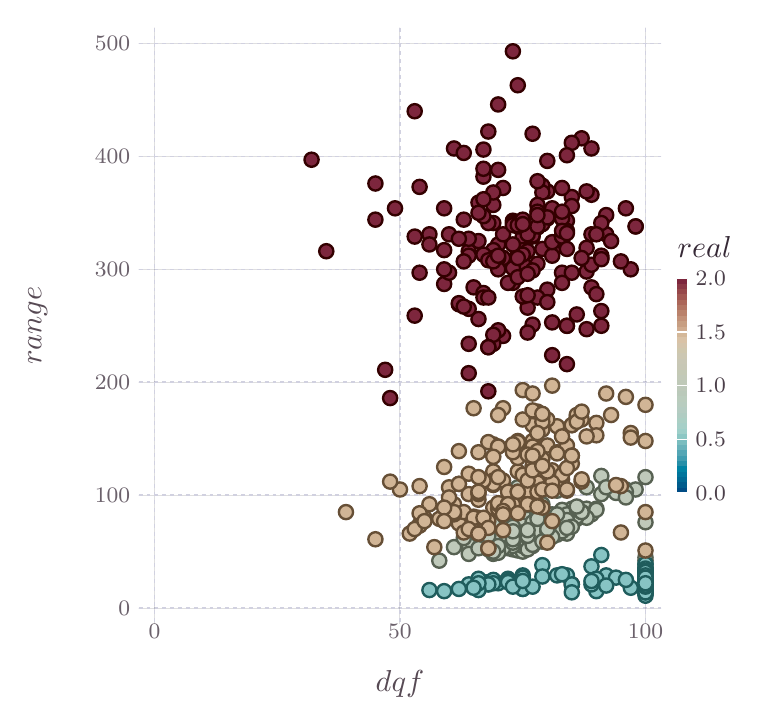
\begin{tikzpicture}[x=1mm,y=-1mm]
\definecolor{mycolorA5CFC7}{rgb}{0.65,0.81,0.78}
\definecolor{mycolor0083A3}{rgb}{0,0.51,0.64}
\definecolor{mycolorB7CBBF}{rgb}{0.72,0.8,0.75}
\definecolor{mycolor88C4C4}{rgb}{0.53,0.77,0.77}
\definecolor{mycolor7BBCC0}{rgb}{0.48,0.74,0.75}
\definecolor{mycolorAA665A}{rgb}{0.67,0.4,0.35}
\definecolor{mycolor664F35}{rgb}{0.4,0.31,0.21}
\definecolor{mycolorD2B497}{rgb}{0.82,0.71,0.59}
\definecolor{mycolorB27563}{rgb}{0.7,0.46,0.39}
\definecolor{mycolor1E5C5C}{rgb}{0.12,0.36,0.36}
\definecolor{mycolorC4C9B6}{rgb}{0.77,0.79,0.71}
\definecolor{mycolorC6C8B5}{rgb}{0.78,0.78,0.71}
\definecolor{mycolorBBCBBB}{rgb}{0.73,0.79,0.73}
\definecolor{mycolor96484A}{rgb}{0.59,0.28,0.29}
\definecolor{mycolor564A55}{rgb}{0.34,0.29,0.33}
\definecolor{mycolor004D84}{rgb}{0,0.3,0.52}
\definecolor{mycolor7E273E}{rgb}{0.49,0.15,0.24}
\definecolor{mycolor4C404B}{rgb}{0.3,0.25,0.29}
\definecolor{mycolorB1CCC2}{rgb}{0.69,0.8,0.76}
\definecolor{mycolor005B8D}{rgb}{0,0.36,0.55}
\definecolor{mycolorA05752}{rgb}{0.63,0.34,0.32}
\definecolor{mycolorC19177}{rgb}{0.76,0.57,0.47}
\definecolor{mycolorB5CCC1}{rgb}{0.71,0.8,0.76}
\definecolor{mycolorC89E82}{rgb}{0.78,0.62,0.51}
\definecolor{mycolorBA836C}{rgb}{0.73,0.51,0.42}
\definecolor{mycolorBFCAB8}{rgb}{0.75,0.79,0.72}
\definecolor{mycolorC9C7B4}{rgb}{0.79,0.78,0.71}
\definecolor{mycolorBECAB9}{rgb}{0.75,0.79,0.73}
\definecolor{mycolor8DC6C5}{rgb}{0.55,0.78,0.77}
\definecolor{mycolor000000}{rgb}{0,0,0}
\definecolor{mycolorCDAB8E}{rgb}{0.81,0.67,0.56}
\definecolor{mycolorD3B79A}{rgb}{0.83,0.72,0.6}
\definecolor{mycolor69B2BA}{rgb}{0.41,0.7,0.73}
\definecolor{mycolorD4C5AA}{rgb}{0.83,0.77,0.67}
\definecolor{mycolorABCEC4}{rgb}{0.67,0.81,0.77}
\definecolor{mycolor340000}{rgb}{0.2,0,0}
\definecolor{mycolorFFFFFF}{rgb}{1,1,1}
\definecolor{mycolor006995}{rgb}{0,0.41,0.58}
\definecolor{mycolorB9CBBD}{rgb}{0.73,0.8,0.74}
\definecolor{mycolor278FA9}{rgb}{0.15,0.56,0.66}
\definecolor{mycolor6C606B}{rgb}{0.42,0.38,0.42}
\definecolor{mycolor000000}{rgb}{0,0,0}
\definecolor{mycolor8B3844}{rgb}{0.54,0.22,0.27}
\definecolor{mycolor7E273E}{rgb}{0.49,0.15,0.24}
\definecolor{mycolorD8C3A6}{rgb}{0.85,0.76,0.65}
\definecolor{mycolor362A35}{rgb}{0.21,0.16,0.21}
\definecolor{mycolor409BAF}{rgb}{0.25,0.61,0.69}
\definecolor{mycolorCCC7B2}{rgb}{0.8,0.78,0.7}
\definecolor{mycolor55A7B5}{rgb}{0.33,0.65,0.71}
\definecolor{mycolorD0D0E0}{rgb}{0.82,0.82,0.88}
\definecolor{mycolor9ED0CB}{rgb}{0.62,0.81,0.79}
\definecolor{mycolor00769D}{rgb}{0,0.46,0.61}
\definecolor{mycolorC2C9B7}{rgb}{0.76,0.79,0.72}
\definecolor{mycolor576153}{rgb}{0.34,0.38,0.32}
\definecolor{mycolorBDCABA}{rgb}{0.74,0.79,0.73}
\definecolor{mycolorCFC6AE}{rgb}{0.81,0.78,0.68}
\begin{scope}
\begin{scope}
\draw (52.82,88.39) node [text=mycolor564A55,draw=mycolor000000,draw opacity=0,rotate around={-0: (0,1.81)},inner sep=0.0]{\fontsize{3.88mm}{4.66mm}\selectfont $\text{dqf}$};
\end{scope}
\begin{scope}
\draw (21.63,81.72) node [text=mycolor6C606B,rotate around={-0: (31.18,1.34)},inner sep=0.0]{\fontsize{2.82mm}{3.39mm}\selectfont $\text{0}$};
\draw (52.82,81.72) node [text=mycolor6C606B,rotate around={-0: (0,1.34)},inner sep=0.0]{\fontsize{2.82mm}{3.39mm}\selectfont $\text{50}$};
\draw (84,81.72) node [text=mycolor6C606B,rotate around={-0: (-31.18,1.34)},inner sep=0.0]{\fontsize{2.82mm}{3.39mm}\selectfont $\text{100}$};
\end{scope}
\begin{scope}
\begin{scope}
\draw (90.31,43.64) node [text=mycolor4C404B,rotate around={-0: (4.5,6.83)},right,inner sep=0.0]{\fontsize{2.82mm}{3.39mm}\selectfont $\text{1.5}$};
\draw (90.31,50.47) node [text=mycolor4C404B,rotate around={-0: (4.5,0)},right,inner sep=0.0]{\fontsize{2.82mm}{3.39mm}\selectfont $\text{1.0}$};
\draw (90.31,36.81) node [text=mycolor4C404B,rotate around={-0: (4.5,13.66)},right,inner sep=0.0]{\fontsize{2.82mm}{3.39mm}\selectfont $\text{2.0}$};
\draw (90.31,64.13) node [text=mycolor4C404B,rotate around={-0: (4.5,-13.66)},right,inner sep=0.0]{\fontsize{2.82mm}{3.39mm}\selectfont $\text{0.0}$};
\draw (90.31,57.3) node [text=mycolor4C404B,rotate around={-0: (4.5,-6.83)},right,inner sep=0.0]{\fontsize{2.82mm}{3.39mm}\selectfont $\text{0.5}$};
\end{scope}
\begin{scope}
\path [fill=mycolor004D84,draw=mycolor000000,draw opacity=0] (88,63.44) rectangle +(1.31,0.68);
\path [fill=mycolor005B8D,draw=mycolor000000,draw opacity=0] (88,62.76) rectangle +(1.31,0.68);
\path [fill=mycolor006995,draw=mycolor000000,draw opacity=0] (88,62.08) rectangle +(1.31,0.68);
\path [fill=mycolor00769D,draw=mycolor000000,draw opacity=0] (88,61.39) rectangle +(1.31,0.68);
\path [fill=mycolor0083A3,draw=mycolor000000,draw opacity=0] (88,60.71) rectangle +(1.31,0.68);
\path [fill=mycolor278FA9,draw=mycolor000000,draw opacity=0] (88,60.03) rectangle +(1.31,0.68);
\path [fill=mycolor409BAF,draw=mycolor000000,draw opacity=0] (88,59.35) rectangle +(1.31,0.68);
\path [fill=mycolor55A7B5,draw=mycolor000000,draw opacity=0] (88,58.66) rectangle +(1.31,0.68);
\path [fill=mycolor69B2BA,draw=mycolor000000,draw opacity=0] (88,57.98) rectangle +(1.31,0.68);
\path [fill=mycolor7BBCC0,draw=mycolor000000,draw opacity=0] (88,57.3) rectangle +(1.31,0.68);
\path [fill=mycolor8DC6C5,draw=mycolor000000,draw opacity=0] (88,56.61) rectangle +(1.31,0.68);
\path [fill=mycolor9ED0CB,draw=mycolor000000,draw opacity=0] (88,55.93) rectangle +(1.31,0.68);
\path [fill=mycolorA5CFC7,draw=mycolor000000,draw opacity=0] (88,55.25) rectangle +(1.31,0.68);
\path [fill=mycolorABCEC4,draw=mycolor000000,draw opacity=0] (88,54.57) rectangle +(1.31,0.68);
\path [fill=mycolorB1CCC2,draw=mycolor000000,draw opacity=0] (88,53.88) rectangle +(1.31,0.68);
\path [fill=mycolorB5CCC1,draw=mycolor000000,draw opacity=0] (88,53.2) rectangle +(1.31,0.68);
\path [fill=mycolorB7CBBF,draw=mycolor000000,draw opacity=0] (88,52.52) rectangle +(1.31,0.68);
\path [fill=mycolorB9CBBD,draw=mycolor000000,draw opacity=0] (88,51.83) rectangle +(1.31,0.68);
\path [fill=mycolorBBCBBB,draw=mycolor000000,draw opacity=0] (88,51.15) rectangle +(1.31,0.68);
\path [fill=mycolorBDCABA,draw=mycolor000000,draw opacity=0] (88,50.47) rectangle +(1.31,0.68);
\path [fill=mycolorBFCAB8,draw=mycolor000000,draw opacity=0] (88,49.79) rectangle +(1.31,0.68);
\path [fill=mycolorC2C9B7,draw=mycolor000000,draw opacity=0] (88,49.1) rectangle +(1.31,0.68);
\path [fill=mycolorC4C9B6,draw=mycolor000000,draw opacity=0] (88,48.42) rectangle +(1.31,0.68);
\path [fill=mycolorC6C8B5,draw=mycolor000000,draw opacity=0] (88,47.74) rectangle +(1.31,0.68);
\path [fill=mycolorC9C7B4,draw=mycolor000000,draw opacity=0] (88,47.06) rectangle +(1.31,0.68);
\path [fill=mycolorCCC7B2,draw=mycolor000000,draw opacity=0] (88,46.37) rectangle +(1.31,0.68);
\path [fill=mycolorCFC6AE,draw=mycolor000000,draw opacity=0] (88,45.69) rectangle +(1.31,0.68);
\path [fill=mycolorD4C5AA,draw=mycolor000000,draw opacity=0] (88,45.01) rectangle +(1.31,0.68);
\path [fill=mycolorD8C3A6,draw=mycolor000000,draw opacity=0] (88,44.32) rectangle +(1.31,0.68);
\path [fill=mycolorD3B79A,draw=mycolor000000,draw opacity=0] (88,43.64) rectangle +(1.31,0.68);
\path [fill=mycolorCDAB8E,draw=mycolor000000,draw opacity=0] (88,42.96) rectangle +(1.31,0.68);
\path [fill=mycolorC89E82,draw=mycolor000000,draw opacity=0] (88,42.28) rectangle +(1.31,0.68);
\path [fill=mycolorC19177,draw=mycolor000000,draw opacity=0] (88,41.59) rectangle +(1.31,0.68);
\path [fill=mycolorBA836C,draw=mycolor000000,draw opacity=0] (88,40.91) rectangle +(1.31,0.68);
\path [fill=mycolorB27563,draw=mycolor000000,draw opacity=0] (88,40.23) rectangle +(1.31,0.68);
\path [fill=mycolorAA665A,draw=mycolor000000,draw opacity=0] (88,39.54) rectangle +(1.31,0.68);
\path [fill=mycolorA05752,draw=mycolor000000,draw opacity=0] (88,38.86) rectangle +(1.31,0.68);
\path [fill=mycolor96484A,draw=mycolor000000,draw opacity=0] (88,38.18) rectangle +(1.31,0.68);
\path [fill=mycolor8B3844,draw=mycolor000000,draw opacity=0] (88,37.5) rectangle +(1.31,0.68);
\path [fill=mycolor7E273E,draw=mycolor000000,draw opacity=0] (88,36.81) rectangle +(1.31,0.68);
\begin{scope}
[line width=0.2mm]
\path [fill=mycolor004D84,draw=mycolorFFFFFF]  (88,43.64) -- (89.31,43.64);
\path [fill=mycolor005B8D,draw=mycolorFFFFFF]  (88,50.47) -- (89.31,50.47);
\path [fill=mycolor006995,draw=mycolorFFFFFF]  (88,36.81) -- (89.31,36.81);
\path [fill=mycolor00769D,draw=mycolorFFFFFF]  (88,64.13) -- (89.31,64.13);
\path [fill=mycolor0083A3,draw=mycolorFFFFFF]  (88,57.3) -- (89.31,57.3);
\end{scope}
\end{scope}
\begin{scope}
\draw (88,32.81) node [text=mycolor362A35,draw=mycolor000000,draw opacity=0,rotate around={-0: (4.5,0.19)},right,inner sep=0.0]{\fontsize{3.88mm}{4.66mm}\selectfont $\text{real}$};
\end{scope}
\end{scope}
\begin{scope}
\clip  (19.63,5) -- (86,5) -- (86,80.72) -- (19.63,80.72);
\begin{scope}
\clip  (19.63,5) -- (86,5) -- (86,80.72) -- (19.63,80.72);
\path [fill=mycolor000000,fill opacity=0,draw=mycolor000000,draw opacity=0] (19.63,5) rectangle +(66.37,75.72);
\end{scope}
\begin{scope}
[dash pattern=on 0.5mm off 0.5mm,line width=0.2mm]
\path [fill=mycolor000000,draw=mycolorD0D0E0]  (19.63,78.72) -- (86,78.72);
\path [fill=mycolor000000,draw=mycolorD0D0E0]  (19.63,64.37) -- (86,64.37);
\path [fill=mycolor000000,draw=mycolorD0D0E0]  (19.63,50.03) -- (86,50.03);
\path [fill=mycolor000000,draw=mycolorD0D0E0]  (19.63,35.69) -- (86,35.69);
\path [fill=mycolor000000,draw=mycolorD0D0E0]  (19.63,21.34) -- (86,21.34);
\path [fill=mycolor000000,draw=mycolorD0D0E0]  (19.63,7) -- (86,7);
\end{scope}
\begin{scope}
[dash pattern=on 0.5mm off 0.5mm,line width=0.2mm]
\path [fill=mycolor000000,draw=mycolorD0D0E0]  (21.63,5) -- (21.63,80.72);
\path [fill=mycolor000000,draw=mycolorD0D0E0]  (52.82,5) -- (52.82,80.72);
\path [fill=mycolor000000,draw=mycolorD0D0E0]  (84,5) -- (84,80.72);
\end{scope}
\begin{scope}
\begin{scope}
\begin{scope}
[line width=0.3mm]
\path [fill=mycolorBECAB9,draw=mycolor576153] (69.66,68.67) circle [radius=0.9];
\path [fill=mycolorBECAB9,draw=mycolor576153] (76.52,66.09) circle [radius=0.9];
\path [fill=mycolorBECAB9,draw=mycolor576153] (72.15,67.96) circle [radius=0.9];
\path [fill=mycolorBECAB9,draw=mycolor576153] (74.64,68.24) circle [radius=0.9];
\path [fill=mycolorBECAB9,draw=mycolor576153] (69.03,69.97) circle [radius=0.9];
\path [fill=mycolorBECAB9,draw=mycolor576153] (80.26,64.09) circle [radius=0.9];
\path [fill=mycolorBECAB9,draw=mycolor576153] (70.9,69.39) circle [radius=0.9];
\path [fill=mycolorBECAB9,draw=mycolor576153] (66.54,68.96) circle [radius=0.9];
\path [fill=mycolorBECAB9,draw=mycolor576153] (65.91,68.24) circle [radius=0.9];
\path [fill=mycolorBECAB9,draw=mycolor576153] (61.55,70.97) circle [radius=0.9];
\path [fill=mycolorBECAB9,draw=mycolor576153] (67.16,70.54) circle [radius=0.9];
\path [fill=mycolorBECAB9,draw=mycolor576153] (72.15,67.1) circle [radius=0.9];
\path [fill=mycolorBECAB9,draw=mycolor576153] (73.4,68.1) circle [radius=0.9];
\path [fill=mycolorBECAB9,draw=mycolor576153] (71.53,68.82) circle [radius=0.9];
\path [fill=mycolorBECAB9,draw=mycolor576153] (62.17,70.97) circle [radius=0.9];
\path [fill=mycolorBECAB9,draw=mycolor576153] (74.64,67.1) circle [radius=0.9];
\path [fill=mycolorBECAB9,draw=mycolor576153] (71.53,68.24) circle [radius=0.9];
\path [fill=mycolorBECAB9,draw=mycolor576153] (69.03,71.11) circle [radius=0.9];
\path [fill=mycolorBECAB9,draw=mycolor576153] (67.16,71.26) circle [radius=0.9];
\path [fill=mycolorBECAB9,draw=mycolor576153] (65.91,68.67) circle [radius=0.9];
\path [fill=mycolorBECAB9,draw=mycolor576153] (66.54,70.25) circle [radius=0.9];
\path [fill=mycolorBECAB9,draw=mycolor576153] (74.64,66.67) circle [radius=0.9];
\path [fill=mycolorBECAB9,draw=mycolor576153] (77.14,66.81) circle [radius=0.9];
\path [fill=mycolorBECAB9,draw=mycolor576153] (72.15,68.96) circle [radius=0.9];
\path [fill=mycolorBECAB9,draw=mycolor576153] (69.66,70.83) circle [radius=0.9];
\path [fill=mycolorBECAB9,draw=mycolor576153] (72.77,67.96) circle [radius=0.9];
\path [fill=mycolorBECAB9,draw=mycolor576153] (70.28,68.96) circle [radius=0.9];
\path [fill=mycolorBECAB9,draw=mycolor576153] (62.79,70.54) circle [radius=0.9];
\path [fill=mycolorBECAB9,draw=mycolor576153] (74.02,67.1) circle [radius=0.9];
\path [fill=mycolorBECAB9,draw=mycolor576153] (65.91,68.67) circle [radius=0.9];
\path [fill=mycolorBECAB9,draw=mycolor576153] (66.54,69.82) circle [radius=0.9];
\path [fill=mycolorBECAB9,draw=mycolor576153] (64.67,71.83) circle [radius=0.9];
\path [fill=mycolorBECAB9,draw=mycolor576153] (84,72.69) circle [radius=0.9];
\path [fill=mycolorBECAB9,draw=mycolor576153] (74.02,67.67) circle [radius=0.9];
\path [fill=mycolorBECAB9,draw=mycolor576153] (74.02,67.53) circle [radius=0.9];
\path [fill=mycolorBECAB9,draw=mycolor576153] (67.78,71.4) circle [radius=0.9];
\path [fill=mycolorBECAB9,draw=mycolor576153] (73.4,66.52) circle [radius=0.9];
\path [fill=mycolorBECAB9,draw=mycolor576153] (65.91,69.39) circle [radius=0.9];
\path [fill=mycolorBECAB9,draw=mycolor576153] (70.28,69.82) circle [radius=0.9];
\path [fill=mycolorBECAB9,draw=mycolor576153] (68.41,71.54) circle [radius=0.9];
\path [fill=mycolorBECAB9,draw=mycolor576153] (65.29,70.97) circle [radius=0.9];
\path [fill=mycolorBECAB9,draw=mycolor576153] (73.4,67.96) circle [radius=0.9];
\path [fill=mycolorBECAB9,draw=mycolor576153] (59.68,70.97) circle [radius=0.9];
\path [fill=mycolorBECAB9,draw=mycolor576153] (72.15,68.1) circle [radius=0.9];
\path [fill=mycolorBECAB9,draw=mycolor576153] (69.03,68.96) circle [radius=0.9];
\path [fill=mycolorBECAB9,draw=mycolor576153] (64.04,70.54) circle [radius=0.9];
\path [fill=mycolorBECAB9,draw=mycolor576153] (84,67.81) circle [radius=0.9];
\path [fill=mycolorBECAB9,draw=mycolor576153] (72.77,67.38) circle [radius=0.9];
\path [fill=mycolorBECAB9,draw=mycolor576153] (67.78,68.39) circle [radius=0.9];
\path [fill=mycolorBECAB9,draw=mycolor576153] (66.54,69.25) circle [radius=0.9];
\path [fill=mycolorBECAB9,draw=mycolor576153] (69.66,67.67) circle [radius=0.9];
\path [fill=mycolorBECAB9,draw=mycolor576153] (78.39,64.23) circle [radius=0.9];
\path [fill=mycolorBECAB9,draw=mycolor576153] (70.9,65.95) circle [radius=0.9];
\path [fill=mycolorBECAB9,draw=mycolor576153] (65.29,70.97) circle [radius=0.9];
\path [fill=mycolorBECAB9,draw=mycolor576153] (65.29,70.54) circle [radius=0.9];
\path [fill=mycolorBECAB9,draw=mycolor576153] (68.41,69.11) circle [radius=0.9];
\path [fill=mycolorBECAB9,draw=mycolor576153] (70.9,69.82) circle [radius=0.9];
\path [fill=mycolorBECAB9,draw=mycolor576153] (76.52,63.37) circle [radius=0.9];
\path [fill=mycolorBECAB9,draw=mycolor576153] (71.53,68.39) circle [radius=0.9];
\path [fill=mycolorBECAB9,draw=mycolor576153] (69.66,70.4) circle [radius=0.9];
\path [fill=mycolorBECAB9,draw=mycolor576153] (81.51,63.65) circle [radius=0.9];
\path [fill=mycolorBECAB9,draw=mycolor576153] (72.77,63.51) circle [radius=0.9];
\path [fill=mycolorBECAB9,draw=mycolor576153] (69.66,70.4) circle [radius=0.9];
\path [fill=mycolorBECAB9,draw=mycolor576153] (74.64,66.38) circle [radius=0.9];
\path [fill=mycolorBECAB9,draw=mycolor576153] (67.78,66.52) circle [radius=0.9];
\path [fill=mycolorBECAB9,draw=mycolor576153] (70.28,68.67) circle [radius=0.9];
\path [fill=mycolorBECAB9,draw=mycolor576153] (75.27,67.38) circle [radius=0.9];
\path [fill=mycolorBECAB9,draw=mycolor576153] (72.15,67.38) circle [radius=0.9];
\path [fill=mycolorBECAB9,draw=mycolor576153] (66.54,71.11) circle [radius=0.9];
\path [fill=mycolorBECAB9,draw=mycolor576153] (65.29,69.25) circle [radius=0.9];
\path [fill=mycolorBECAB9,draw=mycolor576153] (71.53,68.82) circle [radius=0.9];
\path [fill=mycolorBECAB9,draw=mycolor576153] (73.4,68.39) circle [radius=0.9];
\path [fill=mycolorBECAB9,draw=mycolor576153] (69.66,68.1) circle [radius=0.9];
\path [fill=mycolorBECAB9,draw=mycolor576153] (72.15,68.82) circle [radius=0.9];
\path [fill=mycolorBECAB9,draw=mycolor576153] (65.29,67.53) circle [radius=0.9];
\path [fill=mycolorBECAB9,draw=mycolor576153] (70.28,68.1) circle [radius=0.9];
\path [fill=mycolorBECAB9,draw=mycolor576153] (72.15,67.81) circle [radius=0.9];
\path [fill=mycolorBECAB9,draw=mycolor576153] (65.91,67.96) circle [radius=0.9];
\path [fill=mycolorBECAB9,draw=mycolor576153] (77.76,66.09) circle [radius=0.9];
\path [fill=mycolorBECAB9,draw=mycolor576153] (74.02,68.53) circle [radius=0.9];
\path [fill=mycolorBECAB9,draw=mycolor576153] (82.75,63.65) circle [radius=0.9];
\path [fill=mycolorBECAB9,draw=mycolor576153] (71.53,66.81) circle [radius=0.9];
\path [fill=mycolorBECAB9,draw=mycolor576153] (67.16,70.54) circle [radius=0.9];
\path [fill=mycolorBECAB9,draw=mycolor576153] (72.15,68.39) circle [radius=0.9];
\path [fill=mycolorBECAB9,draw=mycolor576153] (72.77,68.39) circle [radius=0.9];
\path [fill=mycolorBECAB9,draw=mycolor576153] (74.64,66.95) circle [radius=0.9];
\path [fill=mycolorBECAB9,draw=mycolor576153] (74.02,66.67) circle [radius=0.9];
\path [fill=mycolorBECAB9,draw=mycolor576153] (71.53,68.39) circle [radius=0.9];
\path [fill=mycolorBECAB9,draw=mycolor576153] (78.39,61.93) circle [radius=0.9];
\path [fill=mycolorBECAB9,draw=mycolor576153] (77.76,66.24) circle [radius=0.9];
\path [fill=mycolorBECAB9,draw=mycolor576153] (68.41,70.83) circle [radius=0.9];
\path [fill=mycolorBECAB9,draw=mycolor576153] (81.51,63.94) circle [radius=0.9];
\path [fill=mycolorBECAB9,draw=mycolor576153] (70.9,70.25) circle [radius=0.9];
\path [fill=mycolorBECAB9,draw=mycolor576153] (67.78,68.67) circle [radius=0.9];
\path [fill=mycolorBECAB9,draw=mycolor576153] (68.41,68.67) circle [radius=0.9];
\path [fill=mycolorBECAB9,draw=mycolor576153] (66.54,70.11) circle [radius=0.9];
\path [fill=mycolorBECAB9,draw=mycolor576153] (81.51,64.66) circle [radius=0.9];
\path [fill=mycolorBECAB9,draw=mycolor576153] (69.66,67.53) circle [radius=0.9];
\path [fill=mycolorBECAB9,draw=mycolor576153] (65.91,68.82) circle [radius=0.9];
\path [fill=mycolorBECAB9,draw=mycolor576153] (72.77,68.1) circle [radius=0.9];
\path [fill=mycolorBECAB9,draw=mycolor576153] (74.64,66.09) circle [radius=0.9];
\path [fill=mycolorBECAB9,draw=mycolor576153] (79.01,63.37) circle [radius=0.9];
\path [fill=mycolorBECAB9,draw=mycolor576153] (70.9,68.39) circle [radius=0.9];
\path [fill=mycolorBECAB9,draw=mycolor576153] (64.67,68.1) circle [radius=0.9];
\path [fill=mycolorBECAB9,draw=mycolor576153] (84,62.08) circle [radius=0.9];
\path [fill=mycolorBECAB9,draw=mycolor576153] (75.89,67.1) circle [radius=0.9];
\path [fill=mycolorBECAB9,draw=mycolor576153] (74.64,67.53) circle [radius=0.9];
\path [fill=mycolorBECAB9,draw=mycolor576153] (71.53,66.81) circle [radius=0.9];
\path [fill=mycolorBECAB9,draw=mycolor576153] (74.64,67.81) circle [radius=0.9];
\path [fill=mycolorBECAB9,draw=mycolor576153] (62.79,69.97) circle [radius=0.9];
\path [fill=mycolorBECAB9,draw=mycolor576153] (62.17,71.11) circle [radius=0.9];
\path [fill=mycolorBECAB9,draw=mycolor576153] (61.55,70.68) circle [radius=0.9];
\path [fill=mycolorBECAB9,draw=mycolor576153] (70.28,68.82) circle [radius=0.9];
\path [fill=mycolorBECAB9,draw=mycolor576153] (69.03,71.26) circle [radius=0.9];
\path [fill=mycolorBECAB9,draw=mycolor576153] (70.28,70.25) circle [radius=0.9];
\path [fill=mycolorBECAB9,draw=mycolor576153] (64.67,70.11) circle [radius=0.9];
\path [fill=mycolorBECAB9,draw=mycolor576153] (70.28,69.97) circle [radius=0.9];
\path [fill=mycolorBECAB9,draw=mycolor576153] (70.28,69.97) circle [radius=0.9];
\path [fill=mycolorBECAB9,draw=mycolor576153] (74.02,69.25) circle [radius=0.9];
\path [fill=mycolorBECAB9,draw=mycolor576153] (67.78,67.67) circle [radius=0.9];
\path [fill=mycolorBECAB9,draw=mycolor576153] (60.92,69.82) circle [radius=0.9];
\path [fill=mycolorBECAB9,draw=mycolor576153] (73.4,68.67) circle [radius=0.9];
\path [fill=mycolorBECAB9,draw=mycolor576153] (72.77,69.39) circle [radius=0.9];
\path [fill=mycolorBECAB9,draw=mycolor576153] (67.78,63.37) circle [radius=0.9];
\path [fill=mycolorBECAB9,draw=mycolor576153] (69.66,69.25) circle [radius=0.9];
\path [fill=mycolorBECAB9,draw=mycolor576153] (68.41,69.11) circle [radius=0.9];
\path [fill=mycolorBECAB9,draw=mycolor576153] (74.02,67.38) circle [radius=0.9];
\path [fill=mycolorBECAB9,draw=mycolor576153] (69.03,69.25) circle [radius=0.9];
\path [fill=mycolorBECAB9,draw=mycolor576153] (69.66,66.67) circle [radius=0.9];
\path [fill=mycolorBECAB9,draw=mycolor576153] (72.15,67.67) circle [radius=0.9];
\path [fill=mycolorBECAB9,draw=mycolor576153] (68.41,69.39) circle [radius=0.9];
\path [fill=mycolorBECAB9,draw=mycolor576153] (67.78,68.67) circle [radius=0.9];
\path [fill=mycolorBECAB9,draw=mycolor576153] (73.4,67.1) circle [radius=0.9];
\path [fill=mycolorBECAB9,draw=mycolor576153] (72.77,63.8) circle [radius=0.9];
\path [fill=mycolorBECAB9,draw=mycolor576153] (69.66,69.11) circle [radius=0.9];
\path [fill=mycolorBECAB9,draw=mycolor576153] (76.52,67.24) circle [radius=0.9];
\path [fill=mycolorBECAB9,draw=mycolor576153] (75.27,67.1) circle [radius=0.9];
\path [fill=mycolorBECAB9,draw=mycolor576153] (72.15,66.81) circle [radius=0.9];
\path [fill=mycolorBECAB9,draw=mycolor576153] (72.15,68.39) circle [radius=0.9];
\path [fill=mycolorBECAB9,draw=mycolor576153] (64.67,71.54) circle [radius=0.9];
\path [fill=mycolorBECAB9,draw=mycolor576153] (67.16,69.11) circle [radius=0.9];
\path [fill=mycolorBECAB9,draw=mycolor576153] (69.03,68.82) circle [radius=0.9];
\path [fill=mycolorBECAB9,draw=mycolor576153] (69.03,67.38) circle [radius=0.9];
\path [fill=mycolorBECAB9,draw=mycolor576153] (67.16,70.83) circle [radius=0.9];
\path [fill=mycolorBECAB9,draw=mycolor576153] (65.91,71.11) circle [radius=0.9];
\path [fill=mycolorBECAB9,draw=mycolor576153] (64.04,71.26) circle [radius=0.9];
\path [fill=mycolorBECAB9,draw=mycolor576153] (72.77,67.1) circle [radius=0.9];
\path [fill=mycolorBECAB9,draw=mycolor576153] (74.02,68.39) circle [radius=0.9];
\path [fill=mycolorBECAB9,draw=mycolor576153] (69.03,68.82) circle [radius=0.9];
\path [fill=mycolorBECAB9,draw=mycolor576153] (74.02,66.81) circle [radius=0.9];
\path [fill=mycolorBECAB9,draw=mycolor576153] (69.03,69.11) circle [radius=0.9];
\path [fill=mycolorBECAB9,draw=mycolor576153] (70.28,67.96) circle [radius=0.9];
\path [fill=mycolorBECAB9,draw=mycolor576153] (70.28,66.81) circle [radius=0.9];
\path [fill=mycolorBECAB9,draw=mycolor576153] (70.9,65.52) circle [radius=0.9];
\path [fill=mycolorBECAB9,draw=mycolor576153] (67.16,70.4) circle [radius=0.9];
\path [fill=mycolorBECAB9,draw=mycolor576153] (70.28,68.39) circle [radius=0.9];
\path [fill=mycolorBECAB9,draw=mycolor576153] (73.4,68.53) circle [radius=0.9];
\path [fill=mycolorBECAB9,draw=mycolor576153] (75.89,66.52) circle [radius=0.9];
\path [fill=mycolorBECAB9,draw=mycolor576153] (61.55,71.83) circle [radius=0.9];
\path [fill=mycolorBECAB9,draw=mycolor576153] (69.66,70.68) circle [radius=0.9];
\path [fill=mycolorBECAB9,draw=mycolor576153] (64.67,69.54) circle [radius=0.9];
\path [fill=mycolorBECAB9,draw=mycolor576153] (70.28,68.1) circle [radius=0.9];
\path [fill=mycolorBECAB9,draw=mycolor576153] (65.29,71.69) circle [radius=0.9];
\path [fill=mycolorBECAB9,draw=mycolor576153] (68.41,68.24) circle [radius=0.9];
\path [fill=mycolorBECAB9,draw=mycolor576153] (69.66,67.81) circle [radius=0.9];
\path [fill=mycolorBECAB9,draw=mycolor576153] (62.79,71.11) circle [radius=0.9];
\path [fill=mycolorBECAB9,draw=mycolor576153] (72.77,68.82) circle [radius=0.9];
\path [fill=mycolorBECAB9,draw=mycolor576153] (73.4,66.24) circle [radius=0.9];
\path [fill=mycolorBECAB9,draw=mycolor576153] (73.4,68.96) circle [radius=0.9];
\path [fill=mycolorBECAB9,draw=mycolor576153] (84,72.26) circle [radius=0.9];
\path [fill=mycolorBECAB9,draw=mycolor576153] (74.02,66.81) circle [radius=0.9];
\path [fill=mycolorBECAB9,draw=mycolor576153] (75.27,66.09) circle [radius=0.9];
\path [fill=mycolorBECAB9,draw=mycolor576153] (65.29,70.83) circle [radius=0.9];
\path [fill=mycolorBECAB9,draw=mycolor576153] (57.81,72.69) circle [radius=0.9];
\path [fill=mycolorBECAB9,draw=mycolor576153] (70.9,69.11) circle [radius=0.9];
\path [fill=mycolorBECAB9,draw=mycolor576153] (70.9,69.25) circle [radius=0.9];
\path [fill=mycolorBECAB9,draw=mycolor576153] (71.53,67.67) circle [radius=0.9];
\path [fill=mycolorBECAB9,draw=mycolor576153] (75.89,66.52) circle [radius=0.9];
\path [fill=mycolorBECAB9,draw=mycolor576153] (70.28,69.11) circle [radius=0.9];
\path [fill=mycolorBECAB9,draw=mycolor576153] (74.02,67.53) circle [radius=0.9];
\path [fill=mycolorBECAB9,draw=mycolor576153] (71.53,68.96) circle [radius=0.9];
\path [fill=mycolorBECAB9,draw=mycolor576153] (68.41,69.11) circle [radius=0.9];
\path [fill=mycolorBECAB9,draw=mycolor576153] (70.28,66.81) circle [radius=0.9];
\path [fill=mycolorBECAB9,draw=mycolor576153] (72.15,67.38) circle [radius=0.9];
\path [fill=mycolorBECAB9,draw=mycolor576153] (64.67,71.54) circle [radius=0.9];
\path [fill=mycolorBECAB9,draw=mycolor576153] (70.9,70.25) circle [radius=0.9];
\path [fill=mycolorBECAB9,draw=mycolor576153] (75.27,65.81) circle [radius=0.9];
\path [fill=mycolorBECAB9,draw=mycolor576153] (69.03,69.54) circle [radius=0.9];
\path [fill=mycolorBECAB9,draw=mycolor576153] (72.15,69.68) circle [radius=0.9];
\path [fill=mycolorBECAB9,draw=mycolor576153] (67.16,69.97) circle [radius=0.9];
\path [fill=mycolorBECAB9,draw=mycolor576153] (67.16,68.39) circle [radius=0.9];
\path [fill=mycolorBECAB9,draw=mycolor576153] (84,73.55) circle [radius=0.9];
\path [fill=mycolorBECAB9,draw=mycolor576153] (74.64,68.39) circle [radius=0.9];
\path [fill=mycolorBECAB9,draw=mycolor576153] (69.03,68.82) circle [radius=0.9];
\path [fill=mycolorBECAB9,draw=mycolor576153] (74.02,68.53) circle [radius=0.9];
\path [fill=mycolorBECAB9,draw=mycolor576153] (64.04,69.54) circle [radius=0.9];
\path [fill=mycolorBECAB9,draw=mycolor576153] (70.28,67.38) circle [radius=0.9];
\path [fill=mycolorBECAB9,draw=mycolor576153] (67.16,68.96) circle [radius=0.9];
\path [fill=mycolorBECAB9,draw=mycolor576153] (72.77,66.81) circle [radius=0.9];
\path [fill=mycolorBECAB9,draw=mycolor576153] (71.53,68.67) circle [radius=0.9];
\path [fill=mycolor7E273E,draw=mycolor340000] (74.64,75.7) circle [radius=0.9];
\path [fill=mycolor7E273E,draw=mycolor340000] (76.52,35.97) circle [radius=0.9];
\path [fill=mycolor7E273E,draw=mycolor340000] (50.94,48.45) circle [radius=0.9];
\path [fill=mycolor7E273E,draw=mycolor340000] (79.01,31.24) circle [radius=0.9];
\path [fill=mycolor7E273E,draw=mycolor340000] (77.14,20.34) circle [radius=0.9];
\path [fill=mycolor7E273E,draw=mycolor340000] (70.28,30.38) circle [radius=0.9];
\path [fill=mycolor7E273E,draw=mycolor340000] (59.68,20.34) circle [radius=0.9];
\path [fill=mycolor7E273E,draw=mycolor340000] (64.04,51.18) circle [radius=0.9];
\path [fill=mycolor7E273E,draw=mycolor340000] (65.91,44.15) circle [radius=0.9];
\path [fill=mycolor7E273E,draw=mycolor340000] (75.27,41.42) circle [radius=0.9];
\path [fill=mycolor7E273E,draw=mycolor340000] (72.15,46.59) circle [radius=0.9];
\path [fill=mycolor7E273E,draw=mycolor340000] (82.13,35.69) circle [radius=0.9];
\path [fill=mycolor7E273E,draw=mycolor340000] (58.43,37.55) circle [radius=0.9];
\path [fill=mycolor7E273E,draw=mycolor340000] (75.89,19.05) circle [radius=0.9];
\path [fill=mycolor7E273E,draw=mycolor340000] (69.03,40.56) circle [radius=0.9];
\path [fill=mycolor7E273E,draw=mycolor340000] (77.14,37.98) circle [radius=0.9];
\path [fill=mycolor7E273E,draw=mycolor340000] (43.46,33.39) circle [radius=0.9];
\path [fill=mycolor7E273E,draw=mycolor340000] (72.77,32.82) circle [radius=0.9];
\path [fill=mycolor7E273E,draw=mycolor340000] (62.79,32.1) circle [radius=0.9];
\path [fill=mycolor7E273E,draw=mycolor340000] (68.41,34.83) circle [radius=0.9];
\path [fill=mycolor7E273E,draw=mycolor340000] (67.78,12.31) circle [radius=0.9];
\path [fill=mycolor7E273E,draw=mycolor340000] (61.55,33.39) circle [radius=0.9];
\path [fill=mycolor7E273E,draw=mycolor340000] (59.05,31.24) circle [radius=0.9];
\path [fill=mycolor7E273E,draw=mycolor340000] (55.31,36.12) circle [radius=0.9];
\path [fill=mycolor7E273E,draw=mycolor340000] (62.17,37.98) circle [radius=0.9];
\path [fill=mycolor7E273E,draw=mycolor340000] (71.53,25.79) circle [radius=0.9];
\path [fill=mycolor7E273E,draw=mycolor340000] (65.91,25.36) circle [radius=0.9];
\path [fill=mycolor7E273E,draw=mycolor340000] (62.79,42) circle [radius=0.9];
\path [fill=mycolor7E273E,draw=mycolor340000] (69.66,42.71) circle [radius=0.9];
\path [fill=mycolor7E273E,draw=mycolor340000] (79.01,28.8) circle [radius=0.9];
\path [fill=mycolor7E273E,draw=mycolor340000] (64.67,27.51) circle [radius=0.9];
\path [fill=mycolor7E273E,draw=mycolor340000] (74.64,19.62) circle [radius=0.9];
\path [fill=mycolor7E273E,draw=mycolor340000] (65.29,32.53) circle [radius=0.9];
\path [fill=mycolor7E273E,draw=mycolor340000] (69.66,31.53) circle [radius=0.9];
\path [fill=mycolor7E273E,draw=mycolor340000] (68.41,31.53) circle [radius=0.9];
\path [fill=mycolor7E273E,draw=mycolor340000] (68.41,33.25) circle [radius=0.9];
\path [fill=mycolor7E273E,draw=mycolor340000] (71.53,29.23) circle [radius=0.9];
\path [fill=mycolor7E273E,draw=mycolor340000] (77.14,31.24) circle [radius=0.9];
\path [fill=mycolor7E273E,draw=mycolor340000] (69.66,31.38) circle [radius=0.9];
\path [fill=mycolor7E273E,draw=mycolor340000] (67.16,29.52) circle [radius=0.9];
\path [fill=mycolor7E273E,draw=mycolor340000] (58.43,33.25) circle [radius=0.9];
\path [fill=mycolor7E273E,draw=mycolor340000] (64.67,29.81) circle [radius=0.9];
\path [fill=mycolor7E273E,draw=mycolor340000] (61.55,45.15) circle [radius=0.9];
\path [fill=mycolor7E273E,draw=mycolor340000] (67.16,29.81) circle [radius=0.9];
\path [fill=mycolor7E273E,draw=mycolor340000] (59.05,36.12) circle [radius=0.9];
\path [fill=mycolor7E273E,draw=mycolor340000] (61.55,33.96) circle [radius=0.9];
\path [fill=mycolor7E273E,draw=mycolor340000] (67.16,35.26) circle [radius=0.9];
\path [fill=mycolor7E273E,draw=mycolor340000] (49.7,29.38) circle [radius=0.9];
\path [fill=mycolor7E273E,draw=mycolor340000] (62.79,27.22) circle [radius=0.9];
\path [fill=mycolor7E273E,draw=mycolor340000] (73.4,29.23) circle [radius=0.9];
\path [fill=mycolor7E273E,draw=mycolor340000] (67.16,35.54) circle [radius=0.9];
\path [fill=mycolor7E273E,draw=mycolor340000] (65.29,14.75) circle [radius=0.9];
\path [fill=mycolor7E273E,draw=mycolor340000] (82.75,30.24) circle [radius=0.9];
\path [fill=mycolor7E273E,draw=mycolor340000] (70.28,34.97) circle [radius=0.9];
\path [fill=mycolor7E273E,draw=mycolor340000] (64.67,33.25) circle [radius=0.9];
\path [fill=mycolor7E273E,draw=mycolor340000] (64.67,25.93) circle [radius=0.9];
\path [fill=mycolor7E273E,draw=mycolor340000] (64.04,29.81) circle [radius=0.9];
\path [fill=mycolor7E273E,draw=mycolor340000] (70.9,25.07) circle [radius=0.9];
\path [fill=mycolor7E273E,draw=mycolor340000] (77.14,26.22) circle [radius=0.9];
\path [fill=mycolor7E273E,draw=mycolor340000] (70.9,25.93) circle [radius=0.9];
\path [fill=mycolor7E273E,draw=mycolor340000] (78.39,34.25) circle [radius=0.9];
\path [fill=mycolor7E273E,draw=mycolor340000] (70.28,27.51) circle [radius=0.9];
\path [fill=mycolor7E273E,draw=mycolor340000] (67.78,33.82) circle [radius=0.9];
\path [fill=mycolor7E273E,draw=mycolor340000] (69.03,31.24) circle [radius=0.9];
\path [fill=mycolor7E273E,draw=mycolor340000] (67.78,30.24) circle [radius=0.9];
\path [fill=mycolor7E273E,draw=mycolor340000] (71.53,38.27) circle [radius=0.9];
\path [fill=mycolor7E273E,draw=mycolor340000] (74.64,26.51) circle [radius=0.9];
\path [fill=mycolor7E273E,draw=mycolor340000] (74.02,29.52) circle [radius=0.9];
\path [fill=mycolor7E273E,draw=mycolor340000] (70.9,29.95) circle [radius=0.9];
\path [fill=mycolor7E273E,draw=mycolor340000] (70.28,28.37) circle [radius=0.9];
\path [fill=mycolor7E273E,draw=mycolor340000] (73.4,36.12) circle [radius=0.9];
\path [fill=mycolor7E273E,draw=mycolor340000] (79.63,32.1) circle [radius=0.9];
\path [fill=mycolor7E273E,draw=mycolor340000] (81.51,27.94) circle [radius=0.9];
\path [fill=mycolor7E273E,draw=mycolor340000] (67.78,29.81) circle [radius=0.9];
\path [fill=mycolor7E273E,draw=mycolor340000] (70.9,33.1) circle [radius=0.9];
\path [fill=mycolor7E273E,draw=mycolor340000] (70.28,24.5) circle [radius=0.9];
\path [fill=mycolor7E273E,draw=mycolor340000] (76.52,25.79) circle [radius=0.9];
\path [fill=mycolor7E273E,draw=mycolor340000] (72.15,27.94) circle [radius=0.9];
\path [fill=mycolor7E273E,draw=mycolor340000] (71.53,29.09) circle [radius=0.9];
\path [fill=mycolor7E273E,draw=mycolor340000] (70.28,30.24) circle [radius=0.9];
\path [fill=mycolor7E273E,draw=mycolor340000] (77.14,35.11) circle [radius=0.9];
\path [fill=mycolor7E273E,draw=mycolor340000] (73.4,25.36) circle [radius=0.9];
\path [fill=mycolor7E273E,draw=mycolor340000] (74.02,21.2) circle [radius=0.9];
\path [fill=mycolor7E273E,draw=mycolor340000] (63.42,23.92) circle [radius=0.9];
\path [fill=mycolor7E273E,draw=mycolor340000] (60.92,29.38) circle [radius=0.9];
\path [fill=mycolor7E273E,draw=mycolor340000] (63.42,20.48) circle [radius=0.9];
\path [fill=mycolor7E273E,draw=mycolor340000] (65.91,31.24) circle [radius=0.9];
\path [fill=mycolor7E273E,draw=mycolor340000] (70.28,28.8) circle [radius=0.9];
\path [fill=mycolor7E273E,draw=mycolor340000] (73.4,29.23) circle [radius=0.9];
\path [fill=mycolor7E273E,draw=mycolor340000] (67.16,30.09) circle [radius=0.9];
\path [fill=mycolor7E273E,draw=mycolor340000] (68.41,29.81) circle [radius=0.9];
\path [fill=mycolor7E273E,draw=mycolor340000] (82.75,30.24) circle [radius=0.9];
\path [fill=mycolor7E273E,draw=mycolor340000] (71.53,21.92) circle [radius=0.9];
\path [fill=mycolor7E273E,draw=mycolor340000] (69.03,33.39) circle [radius=0.9];
\path [fill=mycolor7E273E,draw=mycolor340000] (74.02,30.81) circle [radius=0.9];
\path [fill=mycolor7E273E,draw=mycolor340000] (64.67,34.25) circle [radius=0.9];
\path [fill=mycolor7E273E,draw=mycolor340000] (56.56,31.24) circle [radius=0.9];
\path [fill=mycolor7E273E,draw=mycolor340000] (49.7,24.79) circle [radius=0.9];
\path [fill=mycolor7E273E,draw=mycolor340000] (41.59,21.77) circle [radius=0.9];
\path [fill=mycolor7E273E,draw=mycolor340000] (68.41,33.82) circle [radius=0.9];
\path [fill=mycolor7E273E,draw=mycolor340000] (54.69,31.53) circle [radius=0.9];
\path [fill=mycolor7E273E,draw=mycolor340000] (51.57,52.04) circle [radius=0.9];
\path [fill=mycolor7E273E,draw=mycolor340000] (67.16,37.41) circle [radius=0.9];
\path [fill=mycolor7E273E,draw=mycolor340000] (64.04,18.19) circle [radius=0.9];
\path [fill=mycolor7E273E,draw=mycolor340000] (69.03,43.72) circle [radius=0.9];
\path [fill=mycolor7E273E,draw=mycolor340000] (61.55,31.81) circle [radius=0.9];
\path [fill=mycolor7E273E,draw=mycolor340000] (74.64,27.65) circle [radius=0.9];
\path [fill=mycolor7E273E,draw=mycolor340000] (55.31,25.22) circle [radius=0.9];
\path [fill=mycolor7E273E,draw=mycolor340000] (70.28,39.27) circle [radius=0.9];
\path [fill=mycolor7E273E,draw=mycolor340000] (68.41,39.13) circle [radius=0.9];
\path [fill=mycolor7E273E,draw=mycolor340000] (65.29,23.06) circle [radius=0.9];
\path [fill=mycolor7E273E,draw=mycolor340000] (78.39,33.96) circle [radius=0.9];
\path [fill=mycolor7E273E,draw=mycolor340000] (63.42,28.94) circle [radius=0.9];
\path [fill=mycolor7E273E,draw=mycolor340000] (78.39,29.81) circle [radius=0.9];
\path [fill=mycolor7E273E,draw=mycolor340000] (67.16,8) circle [radius=0.9];
\path [fill=mycolor7E273E,draw=mycolor340000] (78.39,42.86) circle [radius=0.9];
\path [fill=mycolor7E273E,draw=mycolor340000] (76.52,43.29) circle [radius=0.9];
\path [fill=mycolor7E273E,draw=mycolor340000] (76.52,32.96) circle [radius=0.9];
\path [fill=mycolor7E273E,draw=mycolor340000] (60.3,40.13) circle [radius=0.9];
\path [fill=mycolor7E273E,draw=mycolor340000] (67.78,30.09) circle [radius=0.9];
\path [fill=mycolor7E273E,draw=mycolor340000] (66.54,37.41) circle [radius=0.9];
\path [fill=mycolor7E273E,draw=mycolor340000] (78.39,34.4) circle [radius=0.9];
\path [fill=mycolor7E273E,draw=mycolor340000] (67.16,32.53) circle [radius=0.9];
\path [fill=mycolor7E273E,draw=mycolor340000] (69.03,38.98) circle [radius=0.9];
\path [fill=mycolor7E273E,draw=mycolor340000] (69.66,18.47) circle [radius=0.9];
\path [fill=mycolor7E273E,draw=mycolor340000] (62.79,28.51) circle [radius=0.9];
\path [fill=mycolor7E273E,draw=mycolor340000] (64.67,45.15) circle [radius=0.9];
\path [fill=mycolor7E273E,draw=mycolor340000] (67.78,34.25) circle [radius=0.9];
\path [fill=mycolor7E273E,draw=mycolor340000] (63.42,33.82) circle [radius=0.9];
\path [fill=mycolor7E273E,draw=mycolor340000] (77.76,31.24) circle [radius=0.9];
\path [fill=mycolor7E273E,draw=mycolor340000] (75.89,34.25) circle [radius=0.9];
\path [fill=mycolor7E273E,draw=mycolor340000] (69.66,35.83) circle [radius=0.9];
\path [fill=mycolor7E273E,draw=mycolor340000] (74.64,36.12) circle [radius=0.9];
\path [fill=mycolor7E273E,draw=mycolor340000] (73.4,32.1) circle [radius=0.9];
\path [fill=mycolor7E273E,draw=mycolor340000] (73.4,37.41) circle [radius=0.9];
\path [fill=mycolor7E273E,draw=mycolor340000] (61.55,40.71) circle [radius=0.9];
\path [fill=mycolor7E273E,draw=mycolor340000] (60.3,39.99) circle [radius=0.9];
\path [fill=mycolor7E273E,draw=mycolor340000] (72.15,42.43) circle [radius=0.9];
\path [fill=mycolor7E273E,draw=mycolor340000] (67.78,36.69) circle [radius=0.9];
\path [fill=mycolor7E273E,draw=mycolor340000] (73.4,28.37) circle [radius=0.9];
\path [fill=mycolor7E273E,draw=mycolor340000] (64.04,34.54) circle [radius=0.9];
\path [fill=mycolor7E273E,draw=mycolor340000] (72.15,33.96) circle [radius=0.9];
\path [fill=mycolor7E273E,draw=mycolor340000] (54.69,41.57) circle [radius=0.9];
\path [fill=mycolor7E273E,draw=mycolor340000] (65.29,43.43) circle [radius=0.9];
\path [fill=mycolor7E273E,draw=mycolor340000] (65.91,34.25) circle [radius=0.9];
\path [fill=mycolor7E273E,draw=mycolor340000] (65.91,34.25) circle [radius=0.9];
\path [fill=mycolor7E273E,draw=mycolor340000] (65.29,34.25) circle [radius=0.9];
\path [fill=mycolor7E273E,draw=mycolor340000] (65.29,35.69) circle [radius=0.9];
\path [fill=mycolor7E273E,draw=mycolor340000] (63.42,38.7) circle [radius=0.9];
\path [fill=mycolor7E273E,draw=mycolor340000] (60.3,31.81) circle [radius=0.9];
\path [fill=mycolor7E273E,draw=mycolor340000] (63.42,26.79) circle [radius=0.9];
\path [fill=mycolor7E273E,draw=mycolor340000] (68.41,29.38) circle [radius=0.9];
\path [fill=mycolor7E273E,draw=mycolor340000] (64.67,34.68) circle [radius=0.9];
\path [fill=mycolor7E273E,draw=mycolor340000] (58.43,35.69) circle [radius=0.9];
\path [fill=mycolor7E273E,draw=mycolor340000] (72.15,32.24) circle [radius=0.9];
\path [fill=mycolor7E273E,draw=mycolor340000] (77.76,38.84) circle [radius=0.9];
\path [fill=mycolor7E273E,draw=mycolor340000] (63.42,39.27) circle [radius=0.9];
\path [fill=mycolor7E273E,draw=mycolor340000] (73.4,31.53) circle [radius=0.9];
\path [fill=mycolor7E273E,draw=mycolor340000] (73.4,31.53) circle [radius=0.9];
\path [fill=mycolor7E273E,draw=mycolor340000] (64.67,44) circle [radius=0.9];
\path [fill=mycolor7E273E,draw=mycolor340000] (80.88,34.68) circle [radius=0.9];
\path [fill=mycolor7E273E,draw=mycolor340000] (74.02,33.1) circle [radius=0.9];
\path [fill=mycolor7E273E,draw=mycolor340000] (60.92,20.91) circle [radius=0.9];
\path [fill=mycolor7E273E,draw=mycolor340000] (60.92,40.42) circle [radius=0.9];
\path [fill=mycolor7E273E,draw=mycolor340000] (73.4,30.81) circle [radius=0.9];
\path [fill=mycolor7E273E,draw=mycolor340000] (64.04,45.58) circle [radius=0.9];
\path [fill=mycolor7E273E,draw=mycolor340000] (64.04,45.58) circle [radius=0.9];
\path [fill=mycolor7E273E,draw=mycolor340000] (61.55,48.88) circle [radius=0.9];
\path [fill=mycolor7E273E,draw=mycolor340000] (71.53,39.85) circle [radius=0.9];
\path [fill=mycolor7E273E,draw=mycolor340000] (60.92,34.68) circle [radius=0.9];
\path [fill=mycolor7E273E,draw=mycolor340000] (74.02,42.86) circle [radius=0.9];
\path [fill=mycolor7E273E,draw=mycolor340000] (74.02,42.86) circle [radius=0.9];
\path [fill=mycolor7E273E,draw=mycolor340000] (58.43,27.94) circle [radius=0.9];
\path [fill=mycolor7E273E,draw=mycolor340000] (69.03,36.26) circle [radius=0.9];
\path [fill=mycolor7E273E,draw=mycolor340000] (63.42,22.92) circle [radius=0.9];
\path [fill=mycolor7E273E,draw=mycolor340000] (64.04,39.27) circle [radius=0.9];
\path [fill=mycolor7E273E,draw=mycolor340000] (52.19,27.94) circle [radius=0.9];
\path [fill=mycolor7E273E,draw=mycolor340000] (78.39,40.99) circle [radius=0.9];
\path [fill=mycolor7E273E,draw=mycolor340000] (74.02,47.73) circle [radius=0.9];
\path [fill=mycolor7E273E,draw=mycolor340000] (54.69,15.61) circle [radius=0.9];
\path [fill=mycolor7E273E,draw=mycolor340000] (65.29,33.96) circle [radius=0.9];
\path [fill=mycolor7E273E,draw=mycolor340000] (74.02,31.1) circle [radius=0.9];
\path [fill=mycolor7E273E,draw=mycolor340000] (56.56,32.53) circle [radius=0.9];
\path [fill=mycolor7E273E,draw=mycolor340000] (68.41,29.95) circle [radius=0.9];
\path [fill=mycolor88C4C4,draw=mycolor1E5C5C] (70.9,73.26) circle [radius=0.9];
\path [fill=mycolor88C4C4,draw=mycolor1E5C5C] (70.9,74.7) circle [radius=0.9];
\path [fill=mycolor88C4C4,draw=mycolor1E5C5C] (84,75.27) circle [radius=0.9];
\path [fill=mycolor88C4C4,draw=mycolor1E5C5C] (65.29,75.56) circle [radius=0.9];
\path [fill=mycolor88C4C4,draw=mycolor1E5C5C] (61.55,75.7) circle [radius=0.9];
\path [fill=mycolor88C4C4,draw=mycolor1E5C5C] (79.01,74.56) circle [radius=0.9];
\path [fill=mycolor88C4C4,draw=mycolor1E5C5C] (84,76.42) circle [radius=0.9];
\path [fill=mycolor88C4C4,draw=mycolor1E5C5C] (64.04,75.42) circle [radius=0.9];
\path [fill=mycolor88C4C4,draw=mycolor1E5C5C] (60.3,76.28) circle [radius=0.9];
\path [fill=mycolor88C4C4,draw=mycolor1E5C5C] (78.39,71.97) circle [radius=0.9];
\path [fill=mycolor88C4C4,draw=mycolor1E5C5C] (84,76.42) circle [radius=0.9];
\path [fill=mycolor88C4C4,draw=mycolor1E5C5C] (68.41,74.56) circle [radius=0.9];
\path [fill=mycolor88C4C4,draw=mycolor1E5C5C] (77.14,73.41) circle [radius=0.9];
\path [fill=mycolor88C4C4,draw=mycolor1E5C5C] (63.42,75.42) circle [radius=0.9];
\path [fill=mycolor88C4C4,draw=mycolor1E5C5C] (66.54,75.27) circle [radius=0.9];
\path [fill=mycolor88C4C4,draw=mycolor1E5C5C] (72.77,74.56) circle [radius=0.9];
\path [fill=mycolor88C4C4,draw=mycolor1E5C5C] (66.54,74.99) circle [radius=0.9];
\path [fill=mycolor88C4C4,draw=mycolor1E5C5C] (77.76,75.13) circle [radius=0.9];
\path [fill=mycolor88C4C4,draw=mycolor1E5C5C] (84,73.98) circle [radius=0.9];
\path [fill=mycolor88C4C4,draw=mycolor1E5C5C] (84,73.12) circle [radius=0.9];
\path [fill=mycolor88C4C4,draw=mycolor1E5C5C] (77.76,76.56) circle [radius=0.9];
\path [fill=mycolor88C4C4,draw=mycolor1E5C5C] (84,76.42) circle [radius=0.9];
\path [fill=mycolor88C4C4,draw=mycolor1E5C5C] (84,75.13) circle [radius=0.9];
\path [fill=mycolor88C4C4,draw=mycolor1E5C5C] (66.54,75.27) circle [radius=0.9];
\path [fill=mycolor88C4C4,draw=mycolor1E5C5C] (68.41,76.28) circle [radius=0.9];
\path [fill=mycolor88C4C4,draw=mycolor1E5C5C] (68.41,74.84) circle [radius=0.9];
\path [fill=mycolor88C4C4,draw=mycolor1E5C5C] (84,76.42) circle [radius=0.9];
\path [fill=mycolor88C4C4,draw=mycolor1E5C5C] (64.04,75.7) circle [radius=0.9];
\path [fill=mycolor88C4C4,draw=mycolor1E5C5C] (84,73.84) circle [radius=0.9];
\path [fill=mycolor88C4C4,draw=mycolor1E5C5C] (68.41,76.28) circle [radius=0.9];
\path [fill=mycolor88C4C4,draw=mycolor1E5C5C] (69.66,75.99) circle [radius=0.9];
\path [fill=mycolor88C4C4,draw=mycolor1E5C5C] (62.79,74.99) circle [radius=0.9];
\path [fill=mycolor88C4C4,draw=mycolor1E5C5C] (84,75.27) circle [radius=0.9];
\path [fill=mycolor88C4C4,draw=mycolor1E5C5C] (84,73.69) circle [radius=0.9];
\path [fill=mycolor88C4C4,draw=mycolor1E5C5C] (64.67,75.13) circle [radius=0.9];
\path [fill=mycolor88C4C4,draw=mycolor1E5C5C] (84,73.98) circle [radius=0.9];
\path [fill=mycolor88C4C4,draw=mycolor1E5C5C] (84,73.98) circle [radius=0.9];
\path [fill=mycolor88C4C4,draw=mycolor1E5C5C] (84,75.13) circle [radius=0.9];
\path [fill=mycolor88C4C4,draw=mycolor1E5C5C] (84,74.99) circle [radius=0.9];
\path [fill=mycolor88C4C4,draw=mycolor1E5C5C] (64.67,75.56) circle [radius=0.9];
\path [fill=mycolor88C4C4,draw=mycolor1E5C5C] (84,73.98) circle [radius=0.9];
\path [fill=mycolor88C4C4,draw=mycolor1E5C5C] (84,74.84) circle [radius=0.9];
\path [fill=mycolor88C4C4,draw=mycolor1E5C5C] (84,76.85) circle [radius=0.9];
\path [fill=mycolor88C4C4,draw=mycolor1E5C5C] (77.76,75.13) circle [radius=0.9];
\path [fill=mycolor88C4C4,draw=mycolor1E5C5C] (66.54,75.42) circle [radius=0.9];
\path [fill=mycolor88C4C4,draw=mycolor1E5C5C] (74.02,74.56) circle [radius=0.9];
\path [fill=mycolor88C4C4,draw=mycolor1E5C5C] (84,73.12) circle [radius=0.9];
\path [fill=mycolor88C4C4,draw=mycolor1E5C5C] (84,74.99) circle [radius=0.9];
\path [fill=mycolor88C4C4,draw=mycolor1E5C5C] (84,74.41) circle [radius=0.9];
\path [fill=mycolor88C4C4,draw=mycolor1E5C5C] (84,75.13) circle [radius=0.9];
\path [fill=mycolor88C4C4,draw=mycolor1E5C5C] (67.16,75.99) circle [radius=0.9];
\path [fill=mycolor88C4C4,draw=mycolor1E5C5C] (84,76.71) circle [radius=0.9];
\path [fill=mycolor88C4C4,draw=mycolor1E5C5C] (84,75.13) circle [radius=0.9];
\path [fill=mycolor88C4C4,draw=mycolor1E5C5C] (77.14,75.7) circle [radius=0.9];
\path [fill=mycolor88C4C4,draw=mycolor1E5C5C] (84,73.98) circle [radius=0.9];
\path [fill=mycolor88C4C4,draw=mycolor1E5C5C] (84,75.27) circle [radius=0.9];
\path [fill=mycolor88C4C4,draw=mycolor1E5C5C] (84,74.13) circle [radius=0.9];
\path [fill=mycolor88C4C4,draw=mycolor1E5C5C] (80.26,74.84) circle [radius=0.9];
\path [fill=mycolor88C4C4,draw=mycolor1E5C5C] (74.64,75.7) circle [radius=0.9];
\path [fill=mycolor88C4C4,draw=mycolor1E5C5C] (64.04,75.7) circle [radius=0.9];
\path [fill=mycolor88C4C4,draw=mycolor1E5C5C] (62.79,76.42) circle [radius=0.9];
\path [fill=mycolor88C4C4,draw=mycolor1E5C5C] (82.13,76.13) circle [radius=0.9];
\path [fill=mycolor88C4C4,draw=mycolor1E5C5C] (84,76.71) circle [radius=0.9];
\path [fill=mycolor88C4C4,draw=mycolor1E5C5C] (84,75.13) circle [radius=0.9];
\path [fill=mycolor88C4C4,draw=mycolor1E5C5C] (81.51,75.13) circle [radius=0.9];
\path [fill=mycolor88C4C4,draw=mycolor1E5C5C] (84,73.69) circle [radius=0.9];
\path [fill=mycolor88C4C4,draw=mycolor1E5C5C] (84,76.42) circle [radius=0.9];
\path [fill=mycolor88C4C4,draw=mycolor1E5C5C] (84,74.13) circle [radius=0.9];
\path [fill=mycolor88C4C4,draw=mycolor1E5C5C] (58.43,76.56) circle [radius=0.9];
\path [fill=mycolor88C4C4,draw=mycolor1E5C5C] (84,77.14) circle [radius=0.9];
\path [fill=mycolor88C4C4,draw=mycolor1E5C5C] (84,74.99) circle [radius=0.9];
\path [fill=mycolor88C4C4,draw=mycolor1E5C5C] (84,76.71) circle [radius=0.9];
\path [fill=mycolor88C4C4,draw=mycolor1E5C5C] (73.4,74.41) circle [radius=0.9];
\path [fill=mycolor88C4C4,draw=mycolor1E5C5C] (84,76.42) circle [radius=0.9];
\path [fill=mycolor88C4C4,draw=mycolor1E5C5C] (84,74.13) circle [radius=0.9];
\path [fill=mycolor88C4C4,draw=mycolor1E5C5C] (84,75.27) circle [radius=0.9];
\path [fill=mycolor88C4C4,draw=mycolor1E5C5C] (84,74.99) circle [radius=0.9];
\path [fill=mycolor88C4C4,draw=mycolor1E5C5C] (56.56,76.42) circle [radius=0.9];
\path [fill=mycolor88C4C4,draw=mycolor1E5C5C] (84,75.27) circle [radius=0.9];
\path [fill=mycolor88C4C4,draw=mycolor1E5C5C] (68.41,75.27) circle [radius=0.9];
\path [fill=mycolor88C4C4,draw=mycolor1E5C5C] (77.76,74.99) circle [radius=0.9];
\path [fill=mycolor88C4C4,draw=mycolor1E5C5C] (79.01,75.85) circle [radius=0.9];
\path [fill=mycolor88C4C4,draw=mycolor1E5C5C] (62.79,75.56) circle [radius=0.9];
\path [fill=mycolor88C4C4,draw=mycolor1E5C5C] (62.17,76.13) circle [radius=0.9];
\path [fill=mycolor88C4C4,draw=mycolor1E5C5C] (84,73.98) circle [radius=0.9];
\path [fill=mycolor88C4C4,draw=mycolor1E5C5C] (84,76.42) circle [radius=0.9];
\path [fill=mycolor88C4C4,draw=mycolor1E5C5C] (84,75.13) circle [radius=0.9];
\path [fill=mycolor88C4C4,draw=mycolor1E5C5C] (84,74.13) circle [radius=0.9];
\path [fill=mycolor88C4C4,draw=mycolor1E5C5C] (77.14,75.27) circle [radius=0.9];
\path [fill=mycolor88C4C4,draw=mycolor1E5C5C] (74.64,76.71) circle [radius=0.9];
\path [fill=mycolor88C4C4,draw=mycolor1E5C5C] (84,75.42) circle [radius=0.9];
\path [fill=mycolor88C4C4,draw=mycolor1E5C5C] (84,75.85) circle [radius=0.9];
\path [fill=mycolor88C4C4,draw=mycolor1E5C5C] (84,76.71) circle [radius=0.9];
\path [fill=mycolor88C4C4,draw=mycolor1E5C5C] (84,75.7) circle [radius=0.9];
\path [fill=mycolor88C4C4,draw=mycolor1E5C5C] (84,74.56) circle [radius=0.9];
\path [fill=mycolor88C4C4,draw=mycolor1E5C5C] (84,75.27) circle [radius=0.9];
\path [fill=mycolor88C4C4,draw=mycolor1E5C5C] (84,75.99) circle [radius=0.9];
\path [fill=mycolor88C4C4,draw=mycolor1E5C5C] (84,75.85) circle [radius=0.9];
\path [fill=mycolor88C4C4,draw=mycolor1E5C5C] (84,74.99) circle [radius=0.9];
\path [fill=mycolor88C4C4,draw=mycolor1E5C5C] (84,75.42) circle [radius=0.9];
\path [fill=mycolor88C4C4,draw=mycolor1E5C5C] (84,75.42) circle [radius=0.9];
\path [fill=mycolor88C4C4,draw=mycolor1E5C5C] (84,74.84) circle [radius=0.9];
\path [fill=mycolor88C4C4,draw=mycolor1E5C5C] (84,75.56) circle [radius=0.9];
\path [fill=mycolorD2B497,draw=mycolor664F35] (75.89,62.65) circle [radius=0.9];
\path [fill=mycolorD2B497,draw=mycolor664F35] (77.76,55.19) circle [radius=0.9];
\path [fill=mycolorD2B497,draw=mycolor664F35] (64.67,57.92) circle [radius=0.9];
\path [fill=mycolorD2B497,draw=mycolor664F35] (79.01,51.46) circle [radius=0.9];
\path [fill=mycolorD2B497,draw=mycolor664F35] (72.77,55.62) circle [radius=0.9];
\path [fill=mycolorD2B497,draw=mycolor664F35] (61.55,64.23) circle [radius=0.9];
\path [fill=mycolorD2B497,draw=mycolor664F35] (67.16,58.35) circle [radius=0.9];
\path [fill=mycolorD2B497,draw=mycolor664F35] (60.3,62.94) circle [radius=0.9];
\path [fill=mycolorD2B497,draw=mycolor664F35] (68.41,65.23) circle [radius=0.9];
\path [fill=mycolorD2B497,draw=mycolor664F35] (55.93,67.24) circle [radius=0.9];
\path [fill=mycolorD2B497,draw=mycolor664F35] (68.41,64.52) circle [radius=0.9];
\path [fill=mycolorD2B497,draw=mycolor664F35] (75.27,54.48) circle [radius=0.9];
\path [fill=mycolorD2B497,draw=mycolor664F35] (52.82,63.65) circle [radius=0.9];
\path [fill=mycolorD2B497,draw=mycolor664F35] (70.9,59.78) circle [radius=0.9];
\path [fill=mycolorD2B497,draw=mycolor664F35] (59.05,63.37) circle [radius=0.9];
\path [fill=mycolorD2B497,draw=mycolor664F35] (65.29,62.08) circle [radius=0.9];
\path [fill=mycolorD2B497,draw=mycolor664F35] (54.06,69.25) circle [radius=0.9];
\path [fill=mycolorD2B497,draw=mycolor664F35] (67.78,61.36) circle [radius=0.9];
\path [fill=mycolorD2B497,draw=mycolor664F35] (69.66,57.49) circle [radius=0.9];
\path [fill=mycolorD2B497,draw=mycolor664F35] (74.64,55.48) circle [radius=0.9];
\path [fill=mycolorD2B497,draw=mycolor664F35] (68.41,61.79) circle [radius=0.9];
\path [fill=mycolorD2B497,draw=mycolor664F35] (71.53,54.76) circle [radius=0.9];
\path [fill=mycolorD2B497,draw=mycolor664F35] (71.53,58.06) circle [radius=0.9];
\path [fill=mycolorD2B497,draw=mycolor664F35] (67.78,58.49) circle [radius=0.9];
\path [fill=mycolorD2B497,draw=mycolor664F35] (56.56,65.52) circle [radius=0.9];
\path [fill=mycolorD2B497,draw=mycolor664F35] (70.9,54.33) circle [radius=0.9];
\path [fill=mycolorD2B497,draw=mycolor664F35] (64.67,63.08) circle [radius=0.9];
\path [fill=mycolorD2B497,draw=mycolor664F35] (55.31,63.22) circle [radius=0.9];
\path [fill=mycolorD2B497,draw=mycolor664F35] (68.41,51.03) circle [radius=0.9];
\path [fill=mycolorD2B497,draw=mycolor664F35] (62.79,58.92) circle [radius=0.9];
\path [fill=mycolorD2B497,draw=mycolor664F35] (60.3,67.96) circle [radius=0.9];
\path [fill=mycolorD2B497,draw=mycolor664F35] (74.64,55.48) circle [radius=0.9];
\path [fill=mycolorD2B497,draw=mycolor664F35] (81.51,51.89) circle [radius=0.9];
\path [fill=mycolorD2B497,draw=mycolor664F35] (65.91,68.82) circle [radius=0.9];
\path [fill=mycolorD2B497,draw=mycolor664F35] (67.78,59.64) circle [radius=0.9];
\path [fill=mycolorD2B497,draw=mycolor664F35] (79.63,54.19) circle [radius=0.9];
\path [fill=mycolorD2B497,draw=mycolor664F35] (75.27,54.19) circle [radius=0.9];
\path [fill=mycolorD2B497,draw=mycolor664F35] (67.78,57.49) circle [radius=0.9];
\path [fill=mycolorD2B497,draw=mycolor664F35] (72.15,61.22) circle [radius=0.9];
\path [fill=mycolorD2B497,draw=mycolor664F35] (55.31,68.1) circle [radius=0.9];
\path [fill=mycolorD2B497,draw=mycolor664F35] (69.66,51.46) circle [radius=0.9];
\path [fill=mycolorD2B497,draw=mycolor664F35] (82.13,56.48) circle [radius=0.9];
\path [fill=mycolorD2B497,draw=mycolor664F35] (70.9,56.05) circle [radius=0.9];
\path [fill=mycolorD2B497,draw=mycolor664F35] (55.31,66.67) circle [radius=0.9];
\path [fill=mycolorD2B497,draw=mycolor664F35] (84,52.9) circle [radius=0.9];
\path [fill=mycolorD2B497,draw=mycolor664F35] (65.91,62.51) circle [radius=0.9];
\path [fill=mycolorD2B497,draw=mycolor664F35] (64.04,57.63) circle [radius=0.9];
\path [fill=mycolorD2B497,draw=mycolor664F35] (70.28,60.64) circle [radius=0.9];
\path [fill=mycolorD2B497,draw=mycolor664F35] (64.67,65.95) circle [radius=0.9];
\path [fill=mycolorD2B497,draw=mycolor664F35] (67.16,65.52) circle [radius=0.9];
\path [fill=mycolorD2B497,draw=mycolor664F35] (65.29,66.09) circle [radius=0.9];
\path [fill=mycolorD2B497,draw=mycolor664F35] (65.91,53.33) circle [radius=0.9];
\path [fill=mycolorD2B497,draw=mycolor664F35] (65.29,65.52) circle [radius=0.9];
\path [fill=mycolorD2B497,draw=mycolor664F35] (60.92,69.11) circle [radius=0.9];
\path [fill=mycolorD2B497,draw=mycolor664F35] (67.78,57.63) circle [radius=0.9];
\path [fill=mycolorD2B497,draw=mycolor664F35] (64.67,61.36) circle [radius=0.9];
\path [fill=mycolorD2B497,draw=mycolor664F35] (62.79,64.95) circle [radius=0.9];
\path [fill=mycolorD2B497,draw=mycolor664F35] (65.91,66.38) circle [radius=0.9];
\path [fill=mycolorD2B497,draw=mycolor664F35] (84,66.52) circle [radius=0.9];
\path [fill=mycolorD2B497,draw=mycolor664F35] (72.77,58.92) circle [radius=0.9];
\path [fill=mycolorD2B497,draw=mycolor664F35] (66.54,63.94) circle [radius=0.9];
\path [fill=mycolorD2B497,draw=mycolor664F35] (75.89,54.76) circle [radius=0.9];
\path [fill=mycolorD2B497,draw=mycolor664F35] (77.76,56.77) circle [radius=0.9];
\path [fill=mycolorD2B497,draw=mycolor664F35] (70.9,63.37) circle [radius=0.9];
\path [fill=mycolorD2B497,draw=mycolor664F35] (62.17,53.33) circle [radius=0.9];
\path [fill=mycolorD2B497,draw=mycolor664F35] (70.28,62.22) circle [radius=0.9];
\path [fill=mycolorD2B497,draw=mycolor664F35] (65.29,65.38) circle [radius=0.9];
\path [fill=mycolorD2B497,draw=mycolor664F35] (65.29,58.2) circle [radius=0.9];
\path [fill=mycolorD2B497,draw=mycolor664F35] (74.02,58.06) circle [radius=0.9];
\path [fill=mycolorD2B497,draw=mycolor664F35] (69.03,63.8) circle [radius=0.9];
\path [fill=mycolorD2B497,draw=mycolor664F35] (75.27,55.05) circle [radius=0.9];
\path [fill=mycolorD2B497,draw=mycolor664F35] (70.28,53.76) circle [radius=0.9];
\path [fill=mycolorD2B497,draw=mycolor664F35] (67.78,63.94) circle [radius=0.9];
\path [fill=mycolorD2B497,draw=mycolor664F35] (73.4,56.91) circle [radius=0.9];
\path [fill=mycolorD2B497,draw=mycolor664F35] (65.29,54.19) circle [radius=0.9];
\path [fill=mycolorD2B497,draw=mycolor664F35] (74.64,59.35) circle [radius=0.9];
\path [fill=mycolorD2B497,draw=mycolor664F35] (64.67,62.51) circle [radius=0.9];
\path [fill=mycolorD2B497,draw=mycolor664F35] (69.66,55.48) circle [radius=0.9];
\path [fill=mycolorD2B497,draw=mycolor664F35] (76.52,56.91) circle [radius=0.9];
\path [fill=mycolorD2B497,draw=mycolor664F35] (55.31,68.24) circle [radius=0.9];
\path [fill=mycolorD2B497,draw=mycolor664F35] (69.66,59.64) circle [radius=0.9];
\path [fill=mycolorD2B497,draw=mycolor664F35] (72.77,59.07) circle [radius=0.9];
\path [fill=mycolorD2B497,draw=mycolor664F35] (70.28,65.52) circle [radius=0.9];
\path [fill=mycolorD2B497,draw=mycolor664F35] (51.57,62.65) circle [radius=0.9];
\path [fill=mycolorD2B497,draw=mycolor664F35] (61.55,61.65) circle [radius=0.9];
\path [fill=mycolorD2B497,draw=mycolor664F35] (64.67,62.94) circle [radius=0.9];
\path [fill=mycolorD2B497,draw=mycolor664F35] (63.42,62.51) circle [radius=0.9];
\path [fill=mycolorD2B497,draw=mycolor664F35] (65.29,58.2) circle [radius=0.9];
\path [fill=mycolorD2B497,draw=mycolor664F35] (71.53,62.94) circle [radius=0.9];
\path [fill=mycolorD2B497,draw=mycolor664F35] (67.16,58.92) circle [radius=0.9];
\path [fill=mycolorD2B497,draw=mycolor664F35] (59.68,65.52) circle [radius=0.9];
\path [fill=mycolorD2B497,draw=mycolor664F35] (57.81,67.38) circle [radius=0.9];
\path [fill=mycolorD2B497,draw=mycolor664F35] (66.54,65.52) circle [radius=0.9];
\path [fill=mycolorD2B497,draw=mycolor664F35] (62.79,64.23) circle [radius=0.9];
\path [fill=mycolorD2B497,draw=mycolor664F35] (69.03,65.52) circle [radius=0.9];
\path [fill=mycolorD2B497,draw=mycolor664F35] (62.17,67.1) circle [radius=0.9];
\path [fill=mycolorD2B497,draw=mycolor664F35] (73.4,62.36) circle [radius=0.9];
\path [fill=mycolorD2B497,draw=mycolor664F35] (60.92,66.52) circle [radius=0.9];
\path [fill=mycolorD2B497,draw=mycolor664F35] (59.68,66.81) circle [radius=0.9];
\path [fill=mycolorD2B497,draw=mycolor664F35] (59.68,66.52) circle [radius=0.9];
\path [fill=mycolorD2B497,draw=mycolor664F35] (72.15,50.46) circle [radius=0.9];
\path [fill=mycolorD2B497,draw=mycolor664F35] (70.28,62.79) circle [radius=0.9];
\path [fill=mycolorD2B497,draw=mycolor664F35] (59.05,64.66) circle [radius=0.9];
\path [fill=mycolorD2B497,draw=mycolor664F35] (65.29,62.08) circle [radius=0.9];
\path [fill=mycolorD2B497,draw=mycolor664F35] (75.89,53.76) circle [radius=0.9];
\path [fill=mycolorD2B497,draw=mycolor664F35] (69.03,62.51) circle [radius=0.9];
\path [fill=mycolorD2B497,draw=mycolor664F35] (73.4,62.94) circle [radius=0.9];
\path [fill=mycolorD2B497,draw=mycolor664F35] (73.4,61.79) circle [radius=0.9];
\path [fill=mycolorD2B497,draw=mycolor664F35] (62.79,67.24) circle [radius=0.9];
\path [fill=mycolorD2B497,draw=mycolor664F35] (71.53,70.4) circle [radius=0.9];
\path [fill=mycolorD2B497,draw=mycolor664F35] (74.02,63.8) circle [radius=0.9];
\path [fill=mycolorD2B497,draw=mycolor664F35] (58.43,65.95) circle [radius=0.9];
\path [fill=mycolorD2B497,draw=mycolor664F35] (70.28,63.94) circle [radius=0.9];
\path [fill=mycolorD2B497,draw=mycolor664F35] (62.79,62.08) circle [radius=0.9];
\path [fill=mycolorD2B497,draw=mycolor664F35] (72.15,62.79) circle [radius=0.9];
\path [fill=mycolorD2B497,draw=mycolor664F35] (74.64,60.36) circle [radius=0.9];
\path [fill=mycolorD2B497,draw=mycolor664F35] (57.18,70.97) circle [radius=0.9];
\path [fill=mycolorD2B497,draw=mycolor664F35] (82.13,57.06) circle [radius=0.9];
\path [fill=mycolorD2B497,draw=mycolor664F35] (66.54,65.52) circle [radius=0.9];
\path [fill=mycolorD2B497,draw=mycolor664F35] (75.89,62.36) circle [radius=0.9];
\path [fill=mycolorD2B497,draw=mycolor664F35] (58.43,67.67) circle [radius=0.9];
\path [fill=mycolorD2B497,draw=mycolor664F35] (54.69,68.67) circle [radius=0.9];
\path [fill=mycolorD2B497,draw=mycolor664F35] (60.3,58.78) circle [radius=0.9];
\path [fill=mycolorD2B497,draw=mycolor664F35] (62.17,67.24) circle [radius=0.9];
\path [fill=mycolorD2B497,draw=mycolor664F35] (64.04,67.67) circle [radius=0.9];
\path [fill=mycolorD2B497,draw=mycolor664F35] (61.55,68.67) circle [radius=0.9];
\path [fill=mycolorD2B497,draw=mycolor664F35] (84,71.4) circle [radius=0.9];
\path [fill=mycolorD2B497,draw=mycolor664F35] (65.91,66.38) circle [radius=0.9];
\path [fill=mycolorD2B497,draw=mycolor664F35] (63.42,67.24) circle [radius=0.9];
\path [fill=mycolorD2B497,draw=mycolor664F35] (74.02,60.93) circle [radius=0.9];
\path [fill=mycolorD2B497,draw=mycolor664F35] (74.02,63.65) circle [radius=0.9];
\path [fill=mycolorD2B497,draw=mycolor664F35] (70.9,55.05) circle [radius=0.9];
\path [fill=mycolorD2B497,draw=mycolor664F35] (71.53,61.36) circle [radius=0.9];
\path [fill=mycolorD2B497,draw=mycolor664F35] (70.9,63.65) circle [radius=0.9];
\path [fill=mycolorD2B497,draw=mycolor664F35] (69.66,58.2) circle [radius=0.9];
\path [fill=mycolorD2B497,draw=mycolor664F35] (67.78,63.94) circle [radius=0.9];
\path [fill=mycolorD2B497,draw=mycolor664F35] (72.15,67.67) circle [radius=0.9];
\path [fill=mycolorD2B497,draw=mycolor664F35] (69.66,60.64) circle [radius=0.9];
\path [fill=mycolorD2B497,draw=mycolor664F35] (67.78,66.67) circle [radius=0.9];
\path [fill=mycolorD2B497,draw=mycolor664F35] (64.04,71.11) circle [radius=0.9];
\path [fill=mycolorD2B497,draw=mycolor664F35] (64.04,71.11) circle [radius=0.9];
\path [fill=mycolorD2B497,draw=mycolor664F35] (49.7,69.97) circle [radius=0.9];
\path [fill=mycolorD2B497,draw=mycolor664F35] (70.28,56.48) circle [radius=0.9];
\path [fill=mycolorD2B497,draw=mycolor664F35] (68.41,54.76) circle [radius=0.9];
\path [fill=mycolorD2B497,draw=mycolor664F35] (80.88,63.22) circle [radius=0.9];
\path [fill=mycolorD2B497,draw=mycolor664F35] (64.67,59.5) circle [radius=0.9];
\path [fill=mycolorD2B497,draw=mycolor664F35] (67.16,57.92) circle [radius=0.9];
\path [fill=mycolorD2B497,draw=mycolor664F35] (45.96,66.52) circle [radius=0.9];
\path [fill=mycolorD2B497,draw=mycolor664F35] (80.88,69.11) circle [radius=0.9];
\path [fill=mycolorD2B497,draw=mycolor664F35] (69.66,53.61) circle [radius=0.9];
\path [fill=mycolorD2B497,draw=mycolor664F35] (60.3,62.94) circle [radius=0.9];
\path [fill=mycolorD2B497,draw=mycolor664F35] (70.9,65.95) circle [radius=0.9];
\path [fill=mycolorD2B497,draw=mycolor664F35] (70.28,58.78) circle [radius=0.9];
\path [fill=mycolorD2B497,draw=mycolor664F35] (84,57.49) circle [radius=0.9];
\path [fill=mycolorD2B497,draw=mycolor664F35] (70.9,54.05) circle [radius=0.9];
\path [fill=mycolorD2B497,draw=mycolor664F35] (69.03,59.21) circle [radius=0.9];
\path [fill=mycolorD2B497,draw=mycolor664F35] (62.79,63.94) circle [radius=0.9];
\path [fill=mycolorD2B497,draw=mycolor664F35] (62.79,63.94) circle [radius=0.9];
\path [fill=mycolorD2B497,draw=mycolor664F35] (58.43,60.79) circle [radius=0.9];
\path [fill=mycolorD2B497,draw=mycolor664F35] (65.91,66.81) circle [radius=0.9];
\path [fill=mycolorD2B497,draw=mycolor664F35] (55.93,67.67) circle [radius=0.9];
\path [fill=mycolorD2B497,draw=mycolor664F35] (69.66,59.35) circle [radius=0.9];
\path [fill=mycolorD2B497,draw=mycolor664F35] (70.28,65.81) circle [radius=0.9];
\path [fill=mycolorD2B497,draw=mycolor664F35] (64.04,68.53) circle [radius=0.9];
\path [fill=mycolorD2B497,draw=mycolor664F35] (72.15,63.8) circle [radius=0.9];
\path [fill=mycolorD2B497,draw=mycolor664F35] (80.26,63.08) circle [radius=0.9];
\path [fill=mycolorD2B497,draw=mycolor664F35] (74.64,59.35) circle [radius=0.9];
\path [fill=mycolorD2B497,draw=mycolor664F35] (69.66,61.22) circle [radius=0.9];
\path [fill=mycolorD2B497,draw=mycolor664F35] (62.79,69.25) circle [radius=0.9];
\path [fill=mycolorD2B497,draw=mycolor664F35] (62.79,69.25) circle [radius=0.9];
\path [fill=mycolorD2B497,draw=mycolor664F35] (70.9,60.64) circle [radius=0.9];
\end{scope}
\end{scope}
\end{scope}
\end{scope}
\begin{scope}
\draw (18.63,78.72) node [text=mycolor6C606B,rotate around={-0: (-2.51,-35.86)},left,inner sep=0.0]{\fontsize{2.82mm}{3.39mm}\selectfont $\text{0}$};
\draw (18.63,64.37) node [text=mycolor6C606B,rotate around={-0: (-2.51,-21.51)},left,inner sep=0.0]{\fontsize{2.82mm}{3.39mm}\selectfont $\text{100}$};
\draw (18.63,50.03) node [text=mycolor6C606B,rotate around={-0: (-2.51,-7.17)},left,inner sep=0.0]{\fontsize{2.82mm}{3.39mm}\selectfont $\text{200}$};
\draw (18.63,35.69) node [text=mycolor6C606B,rotate around={-0: (-2.51,7.17)},left,inner sep=0.0]{\fontsize{2.82mm}{3.39mm}\selectfont $\text{300}$};
\draw (18.63,21.34) node [text=mycolor6C606B,rotate around={-0: (-2.51,21.51)},left,inner sep=0.0]{\fontsize{2.82mm}{3.39mm}\selectfont $\text{400}$};
\draw (18.63,7) node [text=mycolor6C606B,rotate around={-0: (-2.51,35.86)},left,inner sep=0.0]{\fontsize{2.82mm}{3.39mm}\selectfont $\text{500}$};
\end{scope}
\begin{scope}
\draw (8.81,40.86) node [text=mycolor564A55,draw=mycolor000000,draw opacity=0,rotate around={90: (0,2)},inner sep=0.0]{\fontsize{3.88mm}{4.66mm}\selectfont $\text{range}$};
\end{scope}
\end{scope}
\end{tikzpicture}

	\caption{values measured at \SI{0.5}{\metre} to \SI{2}{\metre} real distance}
	\label{range_05_to_2m}
\end{figure}

\begin{figure}[H]
	\centering
	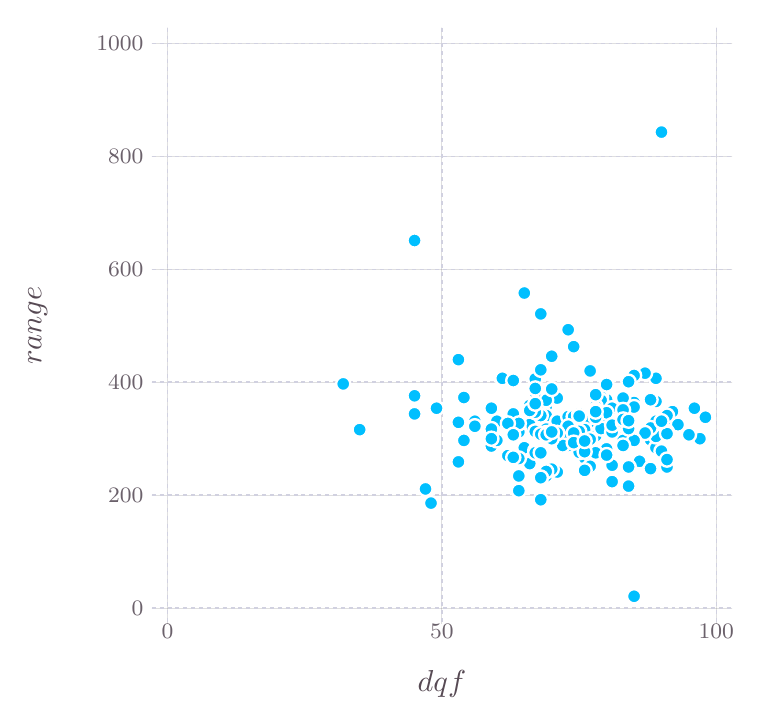
\begin{tikzpicture}[x=1mm,y=-1mm]
\definecolor{mycolor000000}{rgb}{0,0,0}
\definecolor{mycolorFFFFFF}{rgb}{1,1,1}
\definecolor{mycolor564A55}{rgb}{0.34,0.29,0.33}
\definecolor{mycolorD0D0E0}{rgb}{0.82,0.82,0.88}
\definecolor{mycolor000000}{rgb}{0,0,0}
\definecolor{mycolor6C606B}{rgb}{0.42,0.38,0.42}
\definecolor{mycolor00BFFF}{rgb}{0,0.75,1}
\begin{scope}
\begin{scope}
\draw (58.15,88.39) node [text=mycolor564A55,draw=mycolor000000,draw opacity=0,rotate around={-0: (0,1.81)},inner sep=0.0]{\fontsize{3.88mm}{4.66mm}\selectfont $\text{dqf}$};
\end{scope}
\begin{scope}
\draw (23.31,81.72) node [text=mycolor6C606B,rotate around={-0: (34.85,1.34)},inner sep=0.0]{\fontsize{2.82mm}{3.39mm}\selectfont $\text{0}$};
\draw (58.15,81.72) node [text=mycolor6C606B,rotate around={-0: (0,1.34)},inner sep=0.0]{\fontsize{2.82mm}{3.39mm}\selectfont $\text{50}$};
\draw (93,81.72) node [text=mycolor6C606B,rotate around={-0: (-34.85,1.34)},inner sep=0.0]{\fontsize{2.82mm}{3.39mm}\selectfont $\text{100}$};
\end{scope}
\begin{scope}
\clip  (21.31,5) -- (95,5) -- (95,80.72) -- (21.31,80.72);
\begin{scope}
\clip  (21.31,5) -- (95,5) -- (95,80.72) -- (21.31,80.72);
\path [fill=mycolor000000,fill opacity=0,draw=mycolor000000,draw opacity=0] (21.31,5) rectangle +(73.69,75.72);
\end{scope}
\begin{scope}
[dash pattern=on 0.5mm off 0.5mm,line width=0.2mm]
\path [fill=mycolor000000,draw=mycolorD0D0E0]  (21.31,78.72) -- (95,78.72);
\path [fill=mycolor000000,draw=mycolorD0D0E0]  (21.31,64.37) -- (95,64.37);
\path [fill=mycolor000000,draw=mycolorD0D0E0]  (21.31,50.03) -- (95,50.03);
\path [fill=mycolor000000,draw=mycolorD0D0E0]  (21.31,35.69) -- (95,35.69);
\path [fill=mycolor000000,draw=mycolorD0D0E0]  (21.31,21.34) -- (95,21.34);
\path [fill=mycolor000000,draw=mycolorD0D0E0]  (21.31,7) -- (95,7);
\end{scope}
\begin{scope}
[dash pattern=on 0.5mm off 0.5mm,line width=0.2mm]
\path [fill=mycolor000000,draw=mycolorD0D0E0]  (23.31,5) -- (23.31,80.72);
\path [fill=mycolor000000,draw=mycolorD0D0E0]  (58.15,5) -- (58.15,80.72);
\path [fill=mycolor000000,draw=mycolorD0D0E0]  (93,5) -- (93,80.72);
\end{scope}
\begin{scope}
\begin{scope}
\begin{scope}
[line width=0.3mm]
\path [fill=mycolor00BFFF,draw=mycolorFFFFFF] (82.55,77.21) circle [radius=0.9];
\path [fill=mycolor00BFFF,draw=mycolorFFFFFF] (84.64,57.34) circle [radius=0.9];
\path [fill=mycolor00BFFF,draw=mycolorFFFFFF] (56.06,63.58) circle [radius=0.9];
\path [fill=mycolor00BFFF,draw=mycolorFFFFFF] (87.42,54.98) circle [radius=0.9];
\path [fill=mycolor00BFFF,draw=mycolorFFFFFF] (85.33,49.53) circle [radius=0.9];
\path [fill=mycolor00BFFF,draw=mycolorFFFFFF] (77.67,54.55) circle [radius=0.9];
\path [fill=mycolor00BFFF,draw=mycolorFFFFFF] (65.82,49.53) circle [radius=0.9];
\path [fill=mycolor00BFFF,draw=mycolorFFFFFF] (68.61,38.7) circle [radius=0.9];
\path [fill=mycolor00BFFF,draw=mycolorFFFFFF] (70.7,64.95) circle [radius=0.9];
\path [fill=mycolor00BFFF,draw=mycolorFFFFFF] (72.79,61.43) circle [radius=0.9];
\path [fill=mycolor00BFFF,draw=mycolorFFFFFF] (83.24,60.07) circle [radius=0.9];
\path [fill=mycolor00BFFF,draw=mycolorFFFFFF] (79.76,62.65) circle [radius=0.9];
\path [fill=mycolor00BFFF,draw=mycolorFFFFFF] (90.91,57.2) circle [radius=0.9];
\path [fill=mycolor00BFFF,draw=mycolorFFFFFF] (64.43,58.13) circle [radius=0.9];
\path [fill=mycolor00BFFF,draw=mycolorFFFFFF] (83.94,48.88) circle [radius=0.9];
\path [fill=mycolor00BFFF,draw=mycolorFFFFFF] (76.27,59.64) circle [radius=0.9];
\path [fill=mycolor00BFFF,draw=mycolorFFFFFF] (85.33,58.35) circle [radius=0.9];
\path [fill=mycolor00BFFF,draw=mycolorFFFFFF] (47.7,56.05) circle [radius=0.9];
\path [fill=mycolor00BFFF,draw=mycolorFFFFFF] (80.45,55.77) circle [radius=0.9];
\path [fill=mycolor00BFFF,draw=mycolorFFFFFF] (69.3,55.41) circle [radius=0.9];
\path [fill=mycolor00BFFF,draw=mycolorFFFFFF] (75.58,56.77) circle [radius=0.9];
\path [fill=mycolor00BFFF,draw=mycolorFFFFFF] (74.88,45.51) circle [radius=0.9];
\path [fill=mycolor00BFFF,draw=mycolorFFFFFF] (67.91,56.05) circle [radius=0.9];
\path [fill=mycolor00BFFF,draw=mycolorFFFFFF] (65.12,54.98) circle [radius=0.9];
\path [fill=mycolor00BFFF,draw=mycolorFFFFFF] (86.03,18.26) circle [radius=0.9];
\path [fill=mycolor00BFFF,draw=mycolorFFFFFF] (60.94,57.42) circle [radius=0.9];
\path [fill=mycolor00BFFF,draw=mycolorFFFFFF] (68.61,58.35) circle [radius=0.9];
\path [fill=mycolor00BFFF,draw=mycolorFFFFFF] (79.06,52.25) circle [radius=0.9];
\path [fill=mycolor00BFFF,draw=mycolorFFFFFF] (72.79,52.04) circle [radius=0.9];
\path [fill=mycolor00BFFF,draw=mycolorFFFFFF] (69.3,60.36) circle [radius=0.9];
\path [fill=mycolor00BFFF,draw=mycolorFFFFFF] (76.97,60.71) circle [radius=0.9];
\path [fill=mycolor00BFFF,draw=mycolorFFFFFF] (87.42,53.76) circle [radius=0.9];
\path [fill=mycolor00BFFF,draw=mycolorFFFFFF] (71.39,53.11) circle [radius=0.9];
\path [fill=mycolor00BFFF,draw=mycolorFFFFFF] (82.55,49.17) circle [radius=0.9];
\path [fill=mycolor00BFFF,draw=mycolorFFFFFF] (72.09,55.62) circle [radius=0.9];
\path [fill=mycolor00BFFF,draw=mycolorFFFFFF] (76.97,55.12) circle [radius=0.9];
\path [fill=mycolor00BFFF,draw=mycolorFFFFFF] (75.58,55.12) circle [radius=0.9];
\path [fill=mycolor00BFFF,draw=mycolorFFFFFF] (75.58,55.98) circle [radius=0.9];
\path [fill=mycolor00BFFF,draw=mycolorFFFFFF] (79.06,53.97) circle [radius=0.9];
\path [fill=mycolor00BFFF,draw=mycolorFFFFFF] (85.33,54.98) circle [radius=0.9];
\path [fill=mycolor00BFFF,draw=mycolorFFFFFF] (76.97,55.05) circle [radius=0.9];
\path [fill=mycolor00BFFF,draw=mycolorFFFFFF] (74.18,54.12) circle [radius=0.9];
\path [fill=mycolor00BFFF,draw=mycolorFFFFFF] (64.43,55.98) circle [radius=0.9];
\path [fill=mycolor00BFFF,draw=mycolorFFFFFF] (71.39,54.26) circle [radius=0.9];
\path [fill=mycolor00BFFF,draw=mycolorFFFFFF] (67.91,61.93) circle [radius=0.9];
\path [fill=mycolor00BFFF,draw=mycolorFFFFFF] (74.18,54.26) circle [radius=0.9];
\path [fill=mycolor00BFFF,draw=mycolorFFFFFF] (65.12,57.42) circle [radius=0.9];
\path [fill=mycolor00BFFF,draw=mycolorFFFFFF] (67.91,56.34) circle [radius=0.9];
\path [fill=mycolor00BFFF,draw=mycolorFFFFFF] (74.18,56.99) circle [radius=0.9];
\path [fill=mycolor00BFFF,draw=mycolorFFFFFF] (54.67,54.05) circle [radius=0.9];
\path [fill=mycolor00BFFF,draw=mycolorFFFFFF] (69.3,52.97) circle [radius=0.9];
\path [fill=mycolor00BFFF,draw=mycolorFFFFFF] (81.15,53.97) circle [radius=0.9];
\path [fill=mycolor00BFFF,draw=mycolorFFFFFF] (74.18,57.13) circle [radius=0.9];
\path [fill=mycolor00BFFF,draw=mycolorFFFFFF] (72.09,46.73) circle [radius=0.9];
\path [fill=mycolor00BFFF,draw=mycolorFFFFFF] (91.61,54.48) circle [radius=0.9];
\path [fill=mycolor00BFFF,draw=mycolorFFFFFF] (77.67,56.84) circle [radius=0.9];
\path [fill=mycolor00BFFF,draw=mycolorFFFFFF] (71.39,55.98) circle [radius=0.9];
\path [fill=mycolor00BFFF,draw=mycolorFFFFFF] (71.39,52.32) circle [radius=0.9];
\path [fill=mycolor00BFFF,draw=mycolorFFFFFF] (70.7,54.26) circle [radius=0.9];
\path [fill=mycolor00BFFF,draw=mycolorFFFFFF] (78.36,51.89) circle [radius=0.9];
\path [fill=mycolor00BFFF,draw=mycolorFFFFFF] (85.33,52.47) circle [radius=0.9];
\path [fill=mycolor00BFFF,draw=mycolorFFFFFF] (78.36,52.32) circle [radius=0.9];
\path [fill=mycolor00BFFF,draw=mycolorFFFFFF] (86.73,56.48) circle [radius=0.9];
\path [fill=mycolor00BFFF,draw=mycolorFFFFFF] (77.67,53.11) circle [radius=0.9];
\path [fill=mycolor00BFFF,draw=mycolorFFFFFF] (74.88,56.27) circle [radius=0.9];
\path [fill=mycolor00BFFF,draw=mycolorFFFFFF] (76.27,54.98) circle [radius=0.9];
\path [fill=mycolor00BFFF,draw=mycolorFFFFFF] (74.88,54.48) circle [radius=0.9];
\path [fill=mycolor00BFFF,draw=mycolorFFFFFF] (79.06,58.49) circle [radius=0.9];
\path [fill=mycolor00BFFF,draw=mycolorFFFFFF] (82.55,52.61) circle [radius=0.9];
\path [fill=mycolor00BFFF,draw=mycolorFFFFFF] (81.85,54.12) circle [radius=0.9];
\path [fill=mycolor00BFFF,draw=mycolorFFFFFF] (78.36,54.33) circle [radius=0.9];
\path [fill=mycolor00BFFF,draw=mycolorFFFFFF] (77.67,53.54) circle [radius=0.9];
\path [fill=mycolor00BFFF,draw=mycolorFFFFFF] (81.15,57.42) circle [radius=0.9];
\path [fill=mycolor00BFFF,draw=mycolorFFFFFF] (88.12,55.41) circle [radius=0.9];
\path [fill=mycolor00BFFF,draw=mycolorFFFFFF] (90.21,53.33) circle [radius=0.9];
\path [fill=mycolor00BFFF,draw=mycolorFFFFFF] (74.88,54.26) circle [radius=0.9];
\path [fill=mycolor00BFFF,draw=mycolorFFFFFF] (78.36,55.91) circle [radius=0.9];
\path [fill=mycolor00BFFF,draw=mycolorFFFFFF] (77.67,51.61) circle [radius=0.9];
\path [fill=mycolor00BFFF,draw=mycolorFFFFFF] (84.64,52.25) circle [radius=0.9];
\path [fill=mycolor00BFFF,draw=mycolorFFFFFF] (79.76,53.33) circle [radius=0.9];
\path [fill=mycolor00BFFF,draw=mycolorFFFFFF] (79.06,53.9) circle [radius=0.9];
\path [fill=mycolor00BFFF,draw=mycolorFFFFFF] (77.67,54.48) circle [radius=0.9];
\path [fill=mycolor00BFFF,draw=mycolorFFFFFF] (85.33,56.91) circle [radius=0.9];
\path [fill=mycolor00BFFF,draw=mycolorFFFFFF] (81.15,52.04) circle [radius=0.9];
\path [fill=mycolor00BFFF,draw=mycolorFFFFFF] (81.85,49.96) circle [radius=0.9];
\path [fill=mycolor00BFFF,draw=mycolorFFFFFF] (70,51.32) circle [radius=0.9];
\path [fill=mycolor00BFFF,draw=mycolorFFFFFF] (67.21,54.05) circle [radius=0.9];
\path [fill=mycolor00BFFF,draw=mycolorFFFFFF] (70,49.6) circle [radius=0.9];
\path [fill=mycolor00BFFF,draw=mycolorFFFFFF] (72.79,54.98) circle [radius=0.9];
\path [fill=mycolor00BFFF,draw=mycolorFFFFFF] (77.67,53.76) circle [radius=0.9];
\path [fill=mycolor00BFFF,draw=mycolorFFFFFF] (81.15,53.97) circle [radius=0.9];
\path [fill=mycolor00BFFF,draw=mycolorFFFFFF] (74.18,54.4) circle [radius=0.9];
\path [fill=mycolor00BFFF,draw=mycolorFFFFFF] (75.58,54.26) circle [radius=0.9];
\path [fill=mycolor00BFFF,draw=mycolorFFFFFF] (91.61,54.48) circle [radius=0.9];
\path [fill=mycolor00BFFF,draw=mycolorFFFFFF] (79.06,50.32) circle [radius=0.9];
\path [fill=mycolor00BFFF,draw=mycolorFFFFFF] (76.27,56.05) circle [radius=0.9];
\path [fill=mycolor00BFFF,draw=mycolorFFFFFF] (81.85,54.76) circle [radius=0.9];
\path [fill=mycolor00BFFF,draw=mycolorFFFFFF] (71.39,56.48) circle [radius=0.9];
\path [fill=mycolor00BFFF,draw=mycolorFFFFFF] (62.33,54.98) circle [radius=0.9];
\path [fill=mycolor00BFFF,draw=mycolorFFFFFF] (54.67,51.75) circle [radius=0.9];
\path [fill=mycolor00BFFF,draw=mycolorFFFFFF] (45.61,50.24) circle [radius=0.9];
\path [fill=mycolor00BFFF,draw=mycolorFFFFFF] (75.58,56.27) circle [radius=0.9];
\path [fill=mycolor00BFFF,draw=mycolorFFFFFF] (60.24,55.12) circle [radius=0.9];
\path [fill=mycolor00BFFF,draw=mycolorFFFFFF] (56.76,65.38) circle [radius=0.9];
\path [fill=mycolor00BFFF,draw=mycolorFFFFFF] (74.18,58.06) circle [radius=0.9];
\path [fill=mycolor00BFFF,draw=mycolorFFFFFF] (70.7,48.45) circle [radius=0.9];
\path [fill=mycolor00BFFF,draw=mycolorFFFFFF] (76.27,61.22) circle [radius=0.9];
\path [fill=mycolor00BFFF,draw=mycolorFFFFFF] (67.91,55.26) circle [radius=0.9];
\path [fill=mycolor00BFFF,draw=mycolorFFFFFF] (82.55,53.18) circle [radius=0.9];
\path [fill=mycolor00BFFF,draw=mycolorFFFFFF] (60.94,51.97) circle [radius=0.9];
\path [fill=mycolor00BFFF,draw=mycolorFFFFFF] (77.67,58.99) circle [radius=0.9];
\path [fill=mycolor00BFFF,draw=mycolorFFFFFF] (75.58,58.92) circle [radius=0.9];
\path [fill=mycolor00BFFF,draw=mycolorFFFFFF] (72.09,50.89) circle [radius=0.9];
\path [fill=mycolor00BFFF,draw=mycolorFFFFFF] (70.7,41.35) circle [radius=0.9];
\path [fill=mycolor00BFFF,draw=mycolorFFFFFF] (70.7,41.35) circle [radius=0.9];
\path [fill=mycolor00BFFF,draw=mycolorFFFFFF] (86.73,56.34) circle [radius=0.9];
\path [fill=mycolor00BFFF,draw=mycolorFFFFFF] (70,53.83) circle [radius=0.9];
\path [fill=mycolor00BFFF,draw=mycolorFFFFFF] (86.73,54.26) circle [radius=0.9];
\path [fill=mycolor00BFFF,draw=mycolorFFFFFF] (74.18,43.36) circle [radius=0.9];
\path [fill=mycolor00BFFF,draw=mycolorFFFFFF] (86.73,60.79) circle [radius=0.9];
\path [fill=mycolor00BFFF,draw=mycolorFFFFFF] (84.64,61) circle [radius=0.9];
\path [fill=mycolor00BFFF,draw=mycolorFFFFFF] (84.64,55.84) circle [radius=0.9];
\path [fill=mycolor00BFFF,draw=mycolorFFFFFF] (66.52,59.42) circle [radius=0.9];
\path [fill=mycolor00BFFF,draw=mycolorFFFFFF] (74.88,54.4) circle [radius=0.9];
\path [fill=mycolor00BFFF,draw=mycolorFFFFFF] (73.49,58.06) circle [radius=0.9];
\path [fill=mycolor00BFFF,draw=mycolorFFFFFF] (86.73,56.56) circle [radius=0.9];
\path [fill=mycolor00BFFF,draw=mycolorFFFFFF] (74.18,55.62) circle [radius=0.9];
\path [fill=mycolor00BFFF,draw=mycolorFFFFFF] (76.27,58.85) circle [radius=0.9];
\path [fill=mycolor00BFFF,draw=mycolorFFFFFF] (76.97,48.59) circle [radius=0.9];
\path [fill=mycolor00BFFF,draw=mycolorFFFFFF] (69.3,53.61) circle [radius=0.9];
\path [fill=mycolor00BFFF,draw=mycolorFFFFFF] (71.39,61.93) circle [radius=0.9];
\path [fill=mycolor00BFFF,draw=mycolorFFFFFF] (74.88,56.48) circle [radius=0.9];
\path [fill=mycolor00BFFF,draw=mycolorFFFFFF] (70,56.27) circle [radius=0.9];
\path [fill=mycolor00BFFF,draw=mycolorFFFFFF] (86.03,54.98) circle [radius=0.9];
\path [fill=mycolor00BFFF,draw=mycolorFFFFFF] (83.94,56.48) circle [radius=0.9];
\path [fill=mycolor00BFFF,draw=mycolorFFFFFF] (76.97,57.27) circle [radius=0.9];
\path [fill=mycolor00BFFF,draw=mycolorFFFFFF] (82.55,57.42) circle [radius=0.9];
\path [fill=mycolor00BFFF,draw=mycolorFFFFFF] (81.15,55.41) circle [radius=0.9];
\path [fill=mycolor00BFFF,draw=mycolorFFFFFF] (81.15,58.06) circle [radius=0.9];
\path [fill=mycolor00BFFF,draw=mycolorFFFFFF] (67.91,59.71) circle [radius=0.9];
\path [fill=mycolor00BFFF,draw=mycolorFFFFFF] (66.52,59.35) circle [radius=0.9];
\path [fill=mycolor00BFFF,draw=mycolorFFFFFF] (79.76,60.57) circle [radius=0.9];
\path [fill=mycolor00BFFF,draw=mycolorFFFFFF] (74.88,57.7) circle [radius=0.9];
\path [fill=mycolor00BFFF,draw=mycolorFFFFFF] (81.15,53.54) circle [radius=0.9];
\path [fill=mycolor00BFFF,draw=mycolorFFFFFF] (70.7,56.63) circle [radius=0.9];
\path [fill=mycolor00BFFF,draw=mycolorFFFFFF] (79.76,56.34) circle [radius=0.9];
\path [fill=mycolor00BFFF,draw=mycolorFFFFFF] (60.24,60.14) circle [radius=0.9];
\path [fill=mycolor00BFFF,draw=mycolorFFFFFF] (72.09,61.07) circle [radius=0.9];
\path [fill=mycolor00BFFF,draw=mycolorFFFFFF] (72.79,56.48) circle [radius=0.9];
\path [fill=mycolor00BFFF,draw=mycolorFFFFFF] (72.79,56.48) circle [radius=0.9];
\path [fill=mycolor00BFFF,draw=mycolorFFFFFF] (72.09,56.48) circle [radius=0.9];
\path [fill=mycolor00BFFF,draw=mycolorFFFFFF] (72.09,57.2) circle [radius=0.9];
\path [fill=mycolor00BFFF,draw=mycolorFFFFFF] (70,58.71) circle [radius=0.9];
\path [fill=mycolor00BFFF,draw=mycolorFFFFFF] (66.52,55.26) circle [radius=0.9];
\path [fill=mycolor00BFFF,draw=mycolorFFFFFF] (70,52.75) circle [radius=0.9];
\path [fill=mycolor00BFFF,draw=mycolorFFFFFF] (75.58,54.05) circle [radius=0.9];
\path [fill=mycolor00BFFF,draw=mycolorFFFFFF] (71.39,56.7) circle [radius=0.9];
\path [fill=mycolor00BFFF,draw=mycolorFFFFFF] (64.43,57.2) circle [radius=0.9];
\path [fill=mycolor00BFFF,draw=mycolorFFFFFF] (79.76,55.48) circle [radius=0.9];
\path [fill=mycolor00BFFF,draw=mycolorFFFFFF] (86.03,58.78) circle [radius=0.9];
\path [fill=mycolor00BFFF,draw=mycolorFFFFFF] (70,58.99) circle [radius=0.9];
\path [fill=mycolor00BFFF,draw=mycolorFFFFFF] (81.15,55.12) circle [radius=0.9];
\path [fill=mycolor00BFFF,draw=mycolorFFFFFF] (81.15,55.12) circle [radius=0.9];
\path [fill=mycolor00BFFF,draw=mycolorFFFFFF] (71.39,61.36) circle [radius=0.9];
\path [fill=mycolor00BFFF,draw=mycolorFFFFFF] (89.52,56.7) circle [radius=0.9];
\path [fill=mycolor00BFFF,draw=mycolorFFFFFF] (81.85,55.91) circle [radius=0.9];
\path [fill=mycolor00BFFF,draw=mycolorFFFFFF] (67.21,49.81) circle [radius=0.9];
\path [fill=mycolor00BFFF,draw=mycolorFFFFFF] (67.21,59.57) circle [radius=0.9];
\path [fill=mycolor00BFFF,draw=mycolorFFFFFF] (81.15,54.76) circle [radius=0.9];
\path [fill=mycolor00BFFF,draw=mycolorFFFFFF] (70.7,62.15) circle [radius=0.9];
\path [fill=mycolor00BFFF,draw=mycolorFFFFFF] (70.7,62.15) circle [radius=0.9];
\path [fill=mycolor00BFFF,draw=mycolorFFFFFF] (67.91,63.8) circle [radius=0.9];
\path [fill=mycolor00BFFF,draw=mycolorFFFFFF] (79.06,59.28) circle [radius=0.9];
\path [fill=mycolor00BFFF,draw=mycolorFFFFFF] (67.21,56.7) circle [radius=0.9];
\path [fill=mycolor00BFFF,draw=mycolorFFFFFF] (81.85,60.79) circle [radius=0.9];
\path [fill=mycolor00BFFF,draw=mycolorFFFFFF] (81.85,60.79) circle [radius=0.9];
\path [fill=mycolor00BFFF,draw=mycolorFFFFFF] (64.43,53.33) circle [radius=0.9];
\path [fill=mycolor00BFFF,draw=mycolorFFFFFF] (76.27,57.49) circle [radius=0.9];
\path [fill=mycolor00BFFF,draw=mycolorFFFFFF] (70,50.82) circle [radius=0.9];
\path [fill=mycolor00BFFF,draw=mycolorFFFFFF] (70.7,58.99) circle [radius=0.9];
\path [fill=mycolor00BFFF,draw=mycolorFFFFFF] (57.46,53.33) circle [radius=0.9];
\path [fill=mycolor00BFFF,draw=mycolorFFFFFF] (86.73,59.85) circle [radius=0.9];
\path [fill=mycolor00BFFF,draw=mycolorFFFFFF] (81.85,63.22) circle [radius=0.9];
\path [fill=mycolor00BFFF,draw=mycolorFFFFFF] (60.24,47.16) circle [radius=0.9];
\path [fill=mycolor00BFFF,draw=mycolorFFFFFF] (72.09,56.34) circle [radius=0.9];
\path [fill=mycolor00BFFF,draw=mycolorFFFFFF] (81.85,54.91) circle [radius=0.9];
\path [fill=mycolor00BFFF,draw=mycolorFFFFFF] (62.33,55.62) circle [radius=0.9];
\path [fill=mycolor00BFFF,draw=mycolorFFFFFF] (54.67,32.03) circle [radius=0.9];
\path [fill=mycolor00BFFF,draw=mycolorFFFFFF] (75.58,54.33) circle [radius=0.9];
\end{scope}
\end{scope}
\end{scope}
\end{scope}
\begin{scope}
\draw (20.31,78.72) node [text=mycolor6C606B,rotate around={-0: (-3.35,-35.86)},left,inner sep=0.0]{\fontsize{2.82mm}{3.39mm}\selectfont $\text{0}$};
\draw (20.31,64.37) node [text=mycolor6C606B,rotate around={-0: (-3.35,-21.51)},left,inner sep=0.0]{\fontsize{2.82mm}{3.39mm}\selectfont $\text{200}$};
\draw (20.31,50.03) node [text=mycolor6C606B,rotate around={-0: (-3.35,-7.17)},left,inner sep=0.0]{\fontsize{2.82mm}{3.39mm}\selectfont $\text{400}$};
\draw (20.31,35.69) node [text=mycolor6C606B,rotate around={-0: (-3.35,7.17)},left,inner sep=0.0]{\fontsize{2.82mm}{3.39mm}\selectfont $\text{600}$};
\draw (20.31,21.34) node [text=mycolor6C606B,rotate around={-0: (-3.35,21.51)},left,inner sep=0.0]{\fontsize{2.82mm}{3.39mm}\selectfont $\text{800}$};
\draw (20.31,7) node [text=mycolor6C606B,rotate around={-0: (-3.35,35.86)},left,inner sep=0.0]{\fontsize{2.82mm}{3.39mm}\selectfont $\text{1000}$};
\end{scope}
\begin{scope}
\draw (8.81,40.86) node [text=mycolor564A55,draw=mycolor000000,draw opacity=0,rotate around={90: (0,2)},inner sep=0.0]{\fontsize{3.88mm}{4.66mm}\selectfont $\text{range}$};
\end{scope}
\end{scope}
\end{tikzpicture}

	\caption{100 values measured at \SI{2}{\metre} distance}
	\label{2m}
\end{figure}

\subsection{Influence of Input Voltage}

The input voltage has a huge impact on the quality of range values.
This especially means that the battery compartment of the ranging modules must not be used.
\todo{messreihe}

\subsection{Influence of Distance}

It is important to know how the ranging nodes behave at different distances.
In \autoref{boxplot} this relationship is shown.
The results are not what was hoped for when the hardware was selected.
As you can see in \autoref{boxplot} the lower values yielded for any given distance might be in the intervall yielded for pretty much all distances.
Additionaly the mean values are not even nearly monotone, there are some irregularities in the values where a higher distance leads to lower range values.
\todo{prettify}
\begin{landscape}
	\begin{figure}[h]
		\centering
		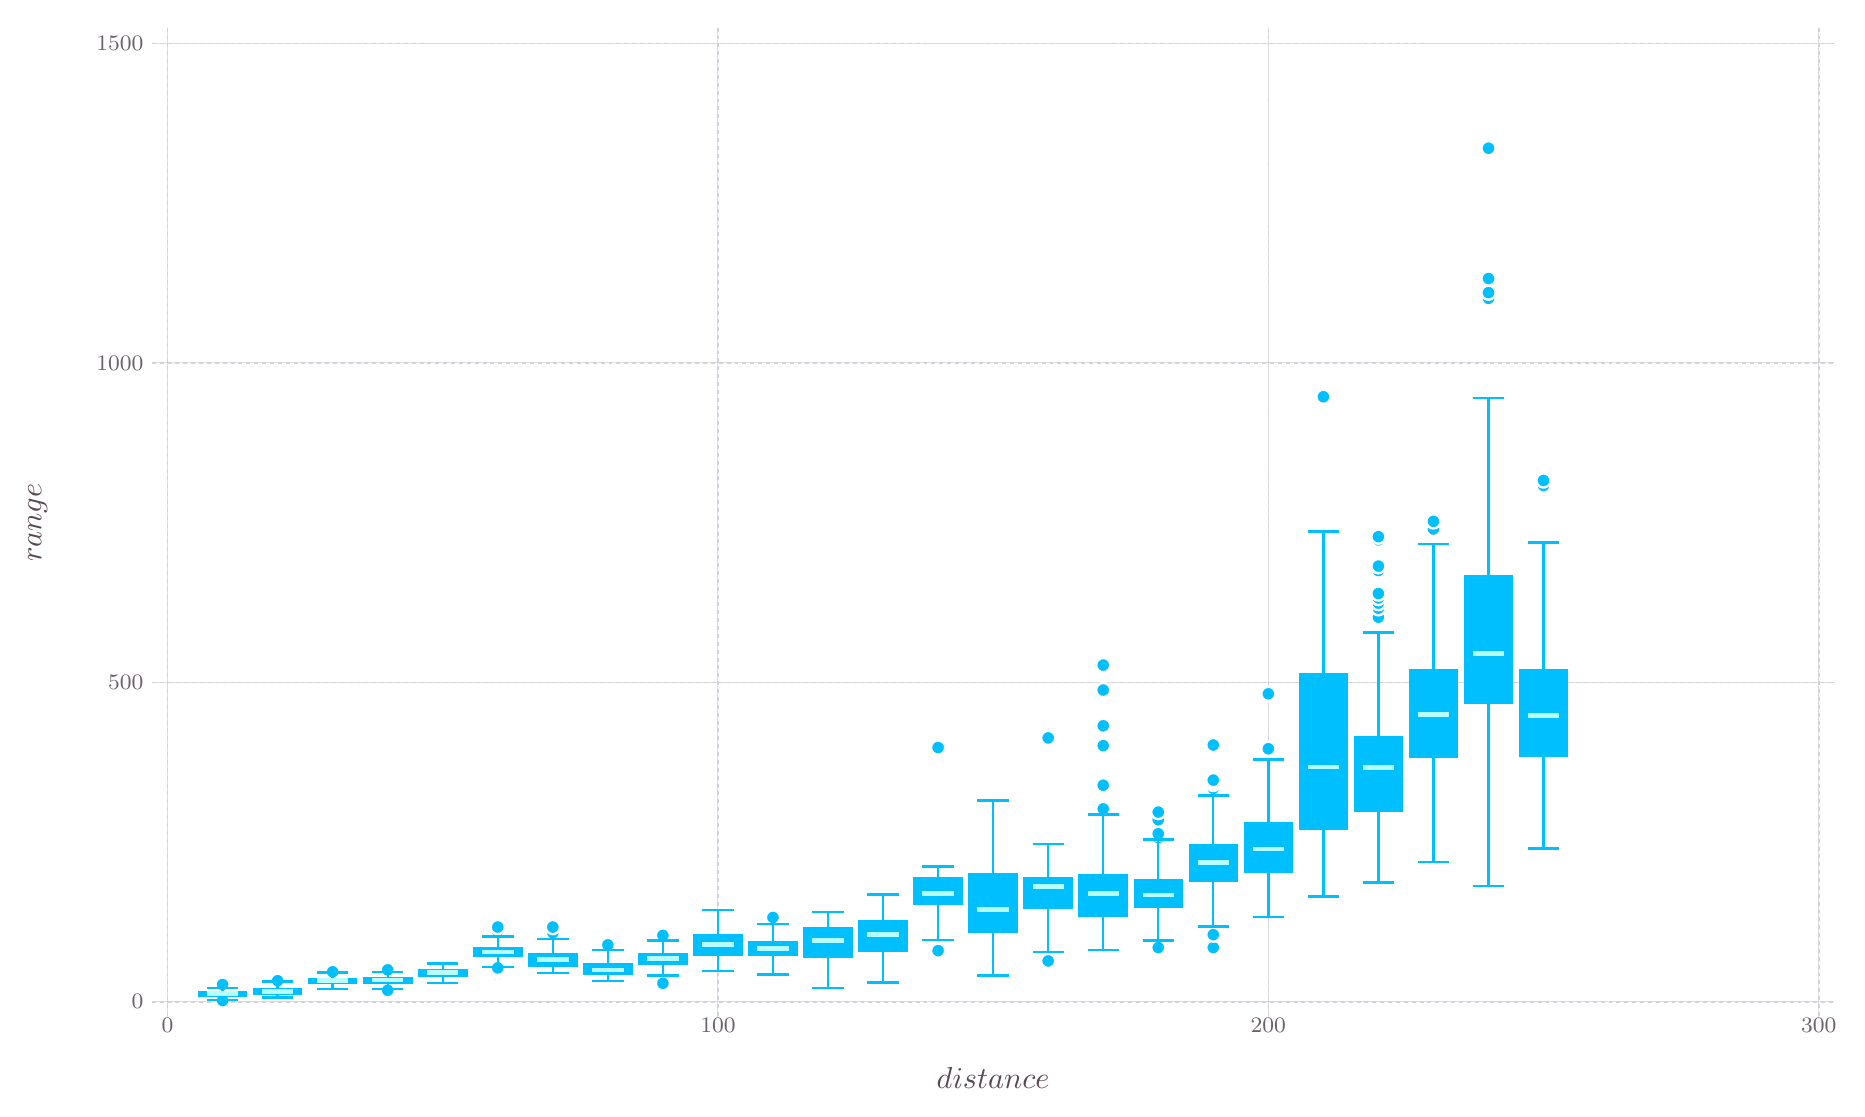
\begin{tikzpicture}[x=1mm,y=-1mm]
\definecolor{mycolorD0D0E0}{rgb}{0.82,0.82,0.88}
\definecolor{mycolor000000}{rgb}{0,0,0}
\definecolor{mycolorB5FFFF}{rgb}{0.71,1,1}
\definecolor{mycolor564A55}{rgb}{0.34,0.29,0.33}
\definecolor{mycolor00BFFF}{rgb}{0,0.75,1}
\definecolor{mycolor000000}{rgb}{0,0,0}
\definecolor{mycolor6C606B}{rgb}{0.42,0.38,0.42}
\definecolor{mycolorFFFFFF}{rgb}{1,1,1}
\begin{scope}
\begin{scope}
\draw (128.15,138.39) node [text=mycolor564A55,draw=mycolor000000,draw opacity=0,rotate around={-0: (0,1.81)},inner sep=0.0]{\fontsize{3.88mm}{4.66mm}\selectfont $\text{distance}$};
\end{scope}
\begin{scope}
\draw (23.31,131.72) node [text=mycolor6C606B,rotate around={-0: (104.85,1.34)},inner sep=0.0]{\fontsize{2.82mm}{3.39mm}\selectfont $\text{0}$};
\draw (93.2,131.72) node [text=mycolor6C606B,rotate around={-0: (34.95,1.34)},inner sep=0.0]{\fontsize{2.82mm}{3.39mm}\selectfont $\text{100}$};
\draw (163.1,131.72) node [text=mycolor6C606B,rotate around={-0: (-34.95,1.34)},inner sep=0.0]{\fontsize{2.82mm}{3.39mm}\selectfont $\text{200}$};
\draw (233,131.72) node [text=mycolor6C606B,rotate around={-0: (-104.85,1.34)},inner sep=0.0]{\fontsize{2.82mm}{3.39mm}\selectfont $\text{300}$};
\end{scope}
\begin{scope}
\clip  (21.31,5) -- (235,5) -- (235,130.72) -- (21.31,130.72);
\begin{scope}
\clip  (21.31,5) -- (235,5) -- (235,130.72) -- (21.31,130.72);
\path [fill=mycolor000000,fill opacity=0,draw=mycolor000000,draw opacity=0] (21.31,5) rectangle +(213.7,125.72);
\end{scope}
\begin{scope}
[dash pattern=on 0.5mm off 0.5mm,line width=0.2mm]
\path [fill=mycolor000000,draw=mycolorD0D0E0]  (21.31,128.71) -- (235,128.71);
\path [fill=mycolor000000,draw=mycolorD0D0E0]  (21.31,88.14) -- (235,88.14);
\path [fill=mycolor000000,draw=mycolorD0D0E0]  (21.31,47.57) -- (235,47.57);
\path [fill=mycolor000000,draw=mycolorD0D0E0]  (21.31,7) -- (235,7);
\end{scope}
\begin{scope}
[dash pattern=on 0.5mm off 0.5mm,line width=0.2mm]
\path [fill=mycolor000000,draw=mycolorD0D0E0]  (23.31,5) -- (23.31,130.72);
\path [fill=mycolor000000,draw=mycolorD0D0E0]  (93.2,5) -- (93.2,130.72);
\path [fill=mycolor000000,draw=mycolorD0D0E0]  (163.1,5) -- (163.1,130.72);
\path [fill=mycolor000000,draw=mycolorD0D0E0]  (233,5) -- (233,130.72);
\end{scope}
\begin{scope}
\begin{scope}
[line width=0.3mm]
\path [fill=mycolor00BFFF,draw=mycolorFFFFFF] (30.29,128.55) circle [radius=0.9];
\path [fill=mycolor00BFFF,draw=mycolorFFFFFF] (30.29,126.85) circle [radius=0.9];
\path [fill=mycolor00BFFF,draw=mycolorFFFFFF] (30.29,126.52) circle [radius=0.9];
\path [fill=mycolor00BFFF,draw=mycolorFFFFFF] (37.28,126.04) circle [radius=0.9];
\path [fill=mycolor00BFFF,draw=mycolorFFFFFF] (44.27,124.9) circle [radius=0.9];
\path [fill=mycolor00BFFF,draw=mycolorFFFFFF] (51.26,127.25) circle [radius=0.9];
\path [fill=mycolor00BFFF,draw=mycolorFFFFFF] (51.26,124.66) circle [radius=0.9];
\path [fill=mycolor00BFFF,draw=mycolorFFFFFF] (51.26,124.66) circle [radius=0.9];
\path [fill=mycolor00BFFF,draw=mycolorFFFFFF] (65.24,125.55) circle [radius=0.9];
\path [fill=mycolor00BFFF,draw=mycolorFFFFFF] (65.24,125.47) circle [radius=0.9];
\path [fill=mycolor00BFFF,draw=mycolorFFFFFF] (65.24,125.39) circle [radius=0.9];
\path [fill=mycolor00BFFF,draw=mycolorFFFFFF] (65.24,125.23) circle [radius=0.9];
\path [fill=mycolor00BFFF,draw=mycolorFFFFFF] (65.24,125.23) circle [radius=0.9];
\path [fill=mycolor00BFFF,draw=mycolorFFFFFF] (65.24,124.9) circle [radius=0.9];
\path [fill=mycolor00BFFF,draw=mycolorFFFFFF] (65.24,124.82) circle [radius=0.9];
\path [fill=mycolor00BFFF,draw=mycolorFFFFFF] (65.24,124.82) circle [radius=0.9];
\path [fill=mycolor00BFFF,draw=mycolorFFFFFF] (65.24,124.82) circle [radius=0.9];
\path [fill=mycolor00BFFF,draw=mycolorFFFFFF] (65.24,124.82) circle [radius=0.9];
\path [fill=mycolor00BFFF,draw=mycolorFFFFFF] (65.24,124.66) circle [radius=0.9];
\path [fill=mycolor00BFFF,draw=mycolorFFFFFF] (65.24,124.66) circle [radius=0.9];
\path [fill=mycolor00BFFF,draw=mycolorFFFFFF] (65.24,124.66) circle [radius=0.9];
\path [fill=mycolor00BFFF,draw=mycolorFFFFFF] (65.24,124.66) circle [radius=0.9];
\path [fill=mycolor00BFFF,draw=mycolorFFFFFF] (65.24,124.66) circle [radius=0.9];
\path [fill=mycolor00BFFF,draw=mycolorFFFFFF] (65.24,124.58) circle [radius=0.9];
\path [fill=mycolor00BFFF,draw=mycolorFFFFFF] (65.24,124.58) circle [radius=0.9];
\path [fill=mycolor00BFFF,draw=mycolorFFFFFF] (65.24,124.41) circle [radius=0.9];
\path [fill=mycolor00BFFF,draw=mycolorFFFFFF] (65.24,120.03) circle [radius=0.9];
\path [fill=mycolor00BFFF,draw=mycolorFFFFFF] (65.24,119.95) circle [radius=0.9];
\path [fill=mycolor00BFFF,draw=mycolorFFFFFF] (65.24,119.71) circle [radius=0.9];
\path [fill=mycolor00BFFF,draw=mycolorFFFFFF] (65.24,119.22) circle [radius=0.9];
\path [fill=mycolor00BFFF,draw=mycolorFFFFFF] (72.23,119.95) circle [radius=0.9];
\path [fill=mycolor00BFFF,draw=mycolorFFFFFF] (72.23,119.22) circle [radius=0.9];
\path [fill=mycolor00BFFF,draw=mycolorFFFFFF] (79.22,121.49) circle [radius=0.9];
\path [fill=mycolor00BFFF,draw=mycolorFFFFFF] (86.21,126.36) circle [radius=0.9];
\path [fill=mycolor00BFFF,draw=mycolorFFFFFF] (86.21,120.52) circle [radius=0.9];
\path [fill=mycolor00BFFF,draw=mycolorFFFFFF] (86.21,120.28) circle [radius=0.9];
\path [fill=mycolor00BFFF,draw=mycolorFFFFFF] (100.19,118.09) circle [radius=0.9];
\path [fill=mycolor00BFFF,draw=mycolorFFFFFF] (100.19,118) circle [radius=0.9];
\path [fill=mycolor00BFFF,draw=mycolorFFFFFF] (121.16,122.22) circle [radius=0.9];
\path [fill=mycolor00BFFF,draw=mycolorFFFFFF] (121.16,96.42) circle [radius=0.9];
\path [fill=mycolor00BFFF,draw=mycolorFFFFFF] (135.14,123.52) circle [radius=0.9];
\path [fill=mycolor00BFFF,draw=mycolorFFFFFF] (135.14,95.2) circle [radius=0.9];
\path [fill=mycolor00BFFF,draw=mycolorFFFFFF] (142.13,104.37) circle [radius=0.9];
\path [fill=mycolor00BFFF,draw=mycolorFFFFFF] (142.13,104.21) circle [radius=0.9];
\path [fill=mycolor00BFFF,draw=mycolorFFFFFF] (142.13,101.21) circle [radius=0.9];
\path [fill=mycolor00BFFF,draw=mycolorFFFFFF] (142.13,96.18) circle [radius=0.9];
\path [fill=mycolor00BFFF,draw=mycolorFFFFFF] (142.13,93.66) circle [radius=0.9];
\path [fill=mycolor00BFFF,draw=mycolorFFFFFF] (142.13,89.12) circle [radius=0.9];
\path [fill=mycolor00BFFF,draw=mycolorFFFFFF] (142.13,85.95) circle [radius=0.9];
\path [fill=mycolor00BFFF,draw=mycolorFFFFFF] (149.12,121.82) circle [radius=0.9];
\path [fill=mycolor00BFFF,draw=mycolorFFFFFF] (149.12,107.86) circle [radius=0.9];
\path [fill=mycolor00BFFF,draw=mycolorFFFFFF] (149.12,107.37) circle [radius=0.9];
\path [fill=mycolor00BFFF,draw=mycolorFFFFFF] (149.12,105.59) circle [radius=0.9];
\path [fill=mycolor00BFFF,draw=mycolorFFFFFF] (149.12,104.62) circle [radius=0.9];
\path [fill=mycolor00BFFF,draw=mycolorFFFFFF] (156.11,121.82) circle [radius=0.9];
\path [fill=mycolor00BFFF,draw=mycolorFFFFFF] (156.11,120.19) circle [radius=0.9];
\path [fill=mycolor00BFFF,draw=mycolorFFFFFF] (156.11,101.86) circle [radius=0.9];
\path [fill=mycolor00BFFF,draw=mycolorFFFFFF] (156.11,101.61) circle [radius=0.9];
\path [fill=mycolor00BFFF,draw=mycolorFFFFFF] (156.11,101.05) circle [radius=0.9];
\path [fill=mycolor00BFFF,draw=mycolorFFFFFF] (156.11,100.88) circle [radius=0.9];
\path [fill=mycolor00BFFF,draw=mycolorFFFFFF] (156.11,100.8) circle [radius=0.9];
\path [fill=mycolor00BFFF,draw=mycolorFFFFFF] (156.11,100.56) circle [radius=0.9];
\path [fill=mycolor00BFFF,draw=mycolorFFFFFF] (156.11,96.1) circle [radius=0.9];
\path [fill=mycolor00BFFF,draw=mycolorFFFFFF] (163.1,96.58) circle [radius=0.9];
\path [fill=mycolor00BFFF,draw=mycolorFFFFFF] (163.1,89.6) circle [radius=0.9];
\path [fill=mycolor00BFFF,draw=mycolorFFFFFF] (170.09,51.87) circle [radius=0.9];
\path [fill=mycolor00BFFF,draw=mycolorFFFFFF] (177.08,79.87) circle [radius=0.9];
\path [fill=mycolor00BFFF,draw=mycolorFFFFFF] (177.08,78.73) circle [radius=0.9];
\path [fill=mycolor00BFFF,draw=mycolorFFFFFF] (177.08,78.08) circle [radius=0.9];
\path [fill=mycolor00BFFF,draw=mycolorFFFFFF] (177.08,77.43) circle [radius=0.9];
\path [fill=mycolor00BFFF,draw=mycolorFFFFFF] (177.08,76.86) circle [radius=0.9];
\path [fill=mycolor00BFFF,draw=mycolorFFFFFF] (177.08,73.94) circle [radius=0.9];
\path [fill=mycolor00BFFF,draw=mycolorFFFFFF] (177.08,73.38) circle [radius=0.9];
\path [fill=mycolor00BFFF,draw=mycolorFFFFFF] (177.08,73.38) circle [radius=0.9];
\path [fill=mycolor00BFFF,draw=mycolorFFFFFF] (177.08,70.05) circle [radius=0.9];
\path [fill=mycolor00BFFF,draw=mycolorFFFFFF] (177.08,69.64) circle [radius=0.9];
\path [fill=mycolor00BFFF,draw=mycolorFFFFFF] (184.07,68.83) circle [radius=0.9];
\path [fill=mycolor00BFFF,draw=mycolorFFFFFF] (184.07,68.67) circle [radius=0.9];
\path [fill=mycolor00BFFF,draw=mycolorFFFFFF] (184.07,67.7) circle [radius=0.9];
\path [fill=mycolor00BFFF,draw=mycolorFFFFFF] (191.06,39.38) circle [radius=0.9];
\path [fill=mycolor00BFFF,draw=mycolorFFFFFF] (191.06,38.65) circle [radius=0.9];
\path [fill=mycolor00BFFF,draw=mycolorFFFFFF] (191.06,36.86) circle [radius=0.9];
\path [fill=mycolor00BFFF,draw=mycolorFFFFFF] (191.06,20.31) circle [radius=0.9];
\path [fill=mycolor00BFFF,draw=mycolorFFFFFF] (198.05,63.15) circle [radius=0.9];
\path [fill=mycolor00BFFF,draw=mycolorFFFFFF] (198.05,62.5) circle [radius=0.9];
\path [fill=mycolor00BFFF,draw=mycolor00BFFF] (27.3,127.5) rectangle +(5.99,0.41);
\path [fill=mycolor00BFFF,draw=mycolor00BFFF] (34.29,127.09) rectangle +(5.99,0.65);
\path [fill=mycolor00BFFF,draw=mycolor00BFFF] (41.28,125.79) rectangle +(5.99,0.57);
\path [fill=mycolor00BFFF,draw=mycolor00BFFF] (48.27,125.71) rectangle +(5.99,0.57);
\path [fill=mycolor00BFFF,draw=mycolor00BFFF] (55.26,124.66) rectangle +(5.99,0.73);
\path [fill=mycolor00BFFF,draw=mycolor00BFFF] (62.25,121.88) rectangle +(5.99,0.99);
\path [fill=mycolor00BFFF,draw=mycolor00BFFF] (69.24,122.71) rectangle +(5.99,1.38);
\path [fill=mycolor00BFFF,draw=mycolor00BFFF] (76.23,123.93) rectangle +(5.99,1.22);
\path [fill=mycolor00BFFF,draw=mycolor00BFFF] (83.22,122.63) rectangle +(5.99,1.3);
\path [fill=mycolor00BFFF,draw=mycolor00BFFF] (90.21,120.19) rectangle +(5.99,2.54);
\path [fill=mycolor00BFFF,draw=mycolor00BFFF] (97.2,121.17) rectangle +(5.99,1.62);
\path [fill=mycolor00BFFF,draw=mycolor00BFFF] (104.19,119.38) rectangle +(5.99,3.57);
\path [fill=mycolor00BFFF,draw=mycolor00BFFF] (111.18,118.49) rectangle +(5.99,3.75);
\path [fill=mycolor00BFFF,draw=mycolor00BFFF] (118.17,113.05) rectangle +(5.99,3.21);
\path [fill=mycolor00BFFF,draw=mycolor00BFFF] (125.16,112.45) rectangle +(5.99,7.34);
\path [fill=mycolor00BFFF,draw=mycolor00BFFF] (132.15,112.97) rectangle +(5.99,3.77);
\path [fill=mycolor00BFFF,draw=mycolor00BFFF] (139.14,112.63) rectangle +(5.99,5.13);
\path [fill=mycolor00BFFF,draw=mycolor00BFFF] (146.13,113.22) rectangle +(5.99,3.41);
\path [fill=mycolor00BFFF,draw=mycolor00BFFF] (153.12,108.88) rectangle +(5.99,4.5);
\path [fill=mycolor00BFFF,draw=mycolor00BFFF] (160.11,106.06) rectangle +(5.99,6.19);
\path [fill=mycolor00BFFF,draw=mycolor00BFFF] (167.1,87.11) rectangle +(5.99,19.62);
\path [fill=mycolor00BFFF,draw=mycolor00BFFF] (174.09,95.08) rectangle +(5.99,9.39);
\path [fill=mycolor00BFFF,draw=mycolor00BFFF] (181.08,86.64) rectangle +(5.99,10.95);
\path [fill=mycolor00BFFF,draw=mycolor00BFFF] (188.07,74.61) rectangle +(5.99,16.15);
\path [fill=mycolor00BFFF,draw=mycolor00BFFF] (195.06,86.6) rectangle +(5.99,10.87);
\path [fill=mycolor00BFFF,draw=mycolor00BFFF]  (28.3,126.93) -- (32.29,126.93);
\path [fill=mycolor00BFFF,draw=mycolor00BFFF]  (35.29,126.12) -- (39.28,126.12);
\path [fill=mycolor00BFFF,draw=mycolor00BFFF]  (42.28,124.98) -- (46.27,124.98);
\path [fill=mycolor00BFFF,draw=mycolor00BFFF]  (49.27,124.9) -- (53.26,124.9);
\path [fill=mycolor00BFFF,draw=mycolor00BFFF]  (56.26,123.85) -- (60.25,123.85);
\path [fill=mycolor00BFFF,draw=mycolor00BFFF]  (63.25,120.44) -- (67.24,120.44);
\path [fill=mycolor00BFFF,draw=mycolor00BFFF]  (70.24,120.76) -- (74.23,120.76);
\path [fill=mycolor00BFFF,draw=mycolor00BFFF]  (77.23,122.14) -- (81.22,122.14);
\path [fill=mycolor00BFFF,draw=mycolor00BFFF]  (84.22,120.93) -- (88.21,120.93);
\path [fill=mycolor00BFFF,draw=mycolor00BFFF]  (91.21,117.03) -- (95.2,117.03);
\path [fill=mycolor00BFFF,draw=mycolor00BFFF]  (98.2,118.82) -- (102.19,118.82);
\path [fill=mycolor00BFFF,draw=mycolor00BFFF]  (105.19,117.27) -- (109.18,117.27);
\path [fill=mycolor00BFFF,draw=mycolor00BFFF]  (112.18,115.08) -- (116.17,115.08);
\path [fill=mycolor00BFFF,draw=mycolor00BFFF]  (119.17,111.51) -- (123.16,111.51);
\path [fill=mycolor00BFFF,draw=mycolor00BFFF]  (126.16,103.15) -- (130.15,103.15);
\path [fill=mycolor00BFFF,draw=mycolor00BFFF]  (133.15,108.67) -- (137.14,108.67);
\path [fill=mycolor00BFFF,draw=mycolor00BFFF]  (140.14,104.94) -- (144.13,104.94);
\path [fill=mycolor00BFFF,draw=mycolor00BFFF]  (147.13,108.1) -- (151.12,108.1);
\path [fill=mycolor00BFFF,draw=mycolor00BFFF]  (154.12,102.51) -- (158.11,102.51);
\path [fill=mycolor00BFFF,draw=mycolor00BFFF]  (161.11,97.96) -- (165.1,97.96);
\path [fill=mycolor00BFFF,draw=mycolor00BFFF]  (168.09,68.99) -- (172.09,68.99);
\path [fill=mycolor00BFFF,draw=mycolor00BFFF]  (175.08,81.81) -- (179.08,81.81);
\path [fill=mycolor00BFFF,draw=mycolor00BFFF]  (182.07,70.54) -- (186.07,70.54);
\path [fill=mycolor00BFFF,draw=mycolor00BFFF]  (189.06,52.03) -- (193.06,52.03);
\path [fill=mycolor00BFFF,draw=mycolor00BFFF]  (196.05,70.37) -- (200.05,70.37);
\path [fill=mycolor00BFFF,draw=mycolor00BFFF]  (28.3,128.47) -- (32.29,128.47);
\path [fill=mycolor00BFFF,draw=mycolor00BFFF]  (35.29,128.15) -- (39.28,128.15);
\path [fill=mycolor00BFFF,draw=mycolor00BFFF]  (42.28,127.09) -- (46.27,127.09);
\path [fill=mycolor00BFFF,draw=mycolor00BFFF]  (49.27,127.09) -- (53.26,127.09);
\path [fill=mycolor00BFFF,draw=mycolor00BFFF]  (56.26,126.36) -- (60.25,126.36);
\path [fill=mycolor00BFFF,draw=mycolor00BFFF]  (63.25,124.33) -- (67.24,124.33);
\path [fill=mycolor00BFFF,draw=mycolor00BFFF]  (70.24,125.06) -- (74.23,125.06);
\path [fill=mycolor00BFFF,draw=mycolor00BFFF]  (77.23,126.04) -- (81.22,126.04);
\path [fill=mycolor00BFFF,draw=mycolor00BFFF]  (84.22,125.39) -- (88.21,125.39);
\path [fill=mycolor00BFFF,draw=mycolor00BFFF]  (91.21,124.82) -- (95.2,124.82);
\path [fill=mycolor00BFFF,draw=mycolor00BFFF]  (98.2,125.23) -- (102.19,125.23);
\path [fill=mycolor00BFFF,draw=mycolor00BFFF]  (105.19,126.93) -- (109.18,126.93);
\path [fill=mycolor00BFFF,draw=mycolor00BFFF]  (112.18,126.28) -- (116.17,126.28);
\path [fill=mycolor00BFFF,draw=mycolor00BFFF]  (119.17,120.84) -- (123.16,120.84);
\path [fill=mycolor00BFFF,draw=mycolor00BFFF]  (126.16,125.39) -- (130.15,125.39);
\path [fill=mycolor00BFFF,draw=mycolor00BFFF]  (133.15,122.39) -- (137.14,122.39);
\path [fill=mycolor00BFFF,draw=mycolor00BFFF]  (140.14,122.14) -- (144.13,122.14);
\path [fill=mycolor00BFFF,draw=mycolor00BFFF]  (147.13,120.93) -- (151.12,120.93);
\path [fill=mycolor00BFFF,draw=mycolor00BFFF]  (154.12,119.14) -- (158.11,119.14);
\path [fill=mycolor00BFFF,draw=mycolor00BFFF]  (161.11,117.92) -- (165.1,117.92);
\path [fill=mycolor00BFFF,draw=mycolor00BFFF]  (168.09,115.33) -- (172.09,115.33);
\path [fill=mycolor00BFFF,draw=mycolor00BFFF]  (175.08,113.54) -- (179.08,113.54);
\path [fill=mycolor00BFFF,draw=mycolor00BFFF]  (182.07,110.94) -- (186.07,110.94);
\path [fill=mycolor00BFFF,draw=mycolor00BFFF]  (189.06,114.03) -- (193.06,114.03);
\path [fill=mycolor00BFFF,draw=mycolor00BFFF]  (196.05,109.24) -- (200.05,109.24);
\path [fill=mycolor00BFFF,draw=mycolor00BFFF]  (30.29,127.5) -- (30.29,126.93);
\path [fill=mycolor00BFFF,draw=mycolor00BFFF]  (37.28,127.09) -- (37.28,126.12);
\path [fill=mycolor00BFFF,draw=mycolor00BFFF]  (44.27,125.79) -- (44.27,124.98);
\path [fill=mycolor00BFFF,draw=mycolor00BFFF]  (51.26,125.71) -- (51.26,124.9);
\path [fill=mycolor00BFFF,draw=mycolor00BFFF]  (58.25,124.66) -- (58.25,123.85);
\path [fill=mycolor00BFFF,draw=mycolor00BFFF]  (65.24,121.88) -- (65.24,120.44);
\path [fill=mycolor00BFFF,draw=mycolor00BFFF]  (72.23,122.71) -- (72.23,120.76);
\path [fill=mycolor00BFFF,draw=mycolor00BFFF]  (79.22,123.93) -- (79.22,122.14);
\path [fill=mycolor00BFFF,draw=mycolor00BFFF]  (86.21,122.63) -- (86.21,120.93);
\path [fill=mycolor00BFFF,draw=mycolor00BFFF]  (93.2,120.19) -- (93.2,117.03);
\path [fill=mycolor00BFFF,draw=mycolor00BFFF]  (100.19,121.17) -- (100.19,118.82);
\path [fill=mycolor00BFFF,draw=mycolor00BFFF]  (107.18,119.38) -- (107.18,117.27);
\path [fill=mycolor00BFFF,draw=mycolor00BFFF]  (114.17,118.49) -- (114.17,115.08);
\path [fill=mycolor00BFFF,draw=mycolor00BFFF]  (121.16,113.05) -- (121.16,111.51);
\path [fill=mycolor00BFFF,draw=mycolor00BFFF]  (128.15,112.45) -- (128.15,103.15);
\path [fill=mycolor00BFFF,draw=mycolor00BFFF]  (135.14,112.97) -- (135.14,108.67);
\path [fill=mycolor00BFFF,draw=mycolor00BFFF]  (142.13,112.63) -- (142.13,104.94);
\path [fill=mycolor00BFFF,draw=mycolor00BFFF]  (149.12,113.22) -- (149.12,108.1);
\path [fill=mycolor00BFFF,draw=mycolor00BFFF]  (156.11,108.88) -- (156.11,102.51);
\path [fill=mycolor00BFFF,draw=mycolor00BFFF]  (163.1,106.06) -- (163.1,97.96);
\path [fill=mycolor00BFFF,draw=mycolor00BFFF]  (170.09,87.11) -- (170.09,68.99);
\path [fill=mycolor00BFFF,draw=mycolor00BFFF]  (177.08,95.08) -- (177.08,81.81);
\path [fill=mycolor00BFFF,draw=mycolor00BFFF]  (184.07,86.64) -- (184.07,70.54);
\path [fill=mycolor00BFFF,draw=mycolor00BFFF]  (191.06,74.61) -- (191.06,52.03);
\path [fill=mycolor00BFFF,draw=mycolor00BFFF]  (198.05,86.6) -- (198.05,70.37);
\path [fill=mycolor00BFFF,draw=mycolor00BFFF]  (30.29,127.9) -- (30.29,128.47);
\path [fill=mycolor00BFFF,draw=mycolor00BFFF]  (37.28,127.74) -- (37.28,128.15);
\path [fill=mycolor00BFFF,draw=mycolor00BFFF]  (44.27,126.36) -- (44.27,127.09);
\path [fill=mycolor00BFFF,draw=mycolor00BFFF]  (51.26,126.28) -- (51.26,127.09);
\path [fill=mycolor00BFFF,draw=mycolor00BFFF]  (58.25,125.39) -- (58.25,126.36);
\path [fill=mycolor00BFFF,draw=mycolor00BFFF]  (65.24,122.87) -- (65.24,124.33);
\path [fill=mycolor00BFFF,draw=mycolor00BFFF]  (72.23,124.09) -- (72.23,125.06);
\path [fill=mycolor00BFFF,draw=mycolor00BFFF]  (79.22,125.14) -- (79.22,126.04);
\path [fill=mycolor00BFFF,draw=mycolor00BFFF]  (86.21,123.93) -- (86.21,125.39);
\path [fill=mycolor00BFFF,draw=mycolor00BFFF]  (93.2,122.73) -- (93.2,124.82);
\path [fill=mycolor00BFFF,draw=mycolor00BFFF]  (100.19,122.79) -- (100.19,125.23);
\path [fill=mycolor00BFFF,draw=mycolor00BFFF]  (107.18,122.95) -- (107.18,126.93);
\path [fill=mycolor00BFFF,draw=mycolor00BFFF]  (114.17,122.24) -- (114.17,126.28);
\path [fill=mycolor00BFFF,draw=mycolor00BFFF]  (121.16,116.26) -- (121.16,120.84);
\path [fill=mycolor00BFFF,draw=mycolor00BFFF]  (128.15,119.79) -- (128.15,125.39);
\path [fill=mycolor00BFFF,draw=mycolor00BFFF]  (135.14,116.75) -- (135.14,122.39);
\path [fill=mycolor00BFFF,draw=mycolor00BFFF]  (142.13,117.76) -- (142.13,122.14);
\path [fill=mycolor00BFFF,draw=mycolor00BFFF]  (149.12,116.62) -- (149.12,120.93);
\path [fill=mycolor00BFFF,draw=mycolor00BFFF]  (156.11,113.38) -- (156.11,119.14);
\path [fill=mycolor00BFFF,draw=mycolor00BFFF]  (163.1,112.24) -- (163.1,117.92);
\path [fill=mycolor00BFFF,draw=mycolor00BFFF]  (170.09,106.73) -- (170.09,115.33);
\path [fill=mycolor00BFFF,draw=mycolor00BFFF]  (177.08,104.47) -- (177.08,113.54);
\path [fill=mycolor00BFFF,draw=mycolor00BFFF]  (184.07,97.6) -- (184.07,110.94);
\path [fill=mycolor00BFFF,draw=mycolor00BFFF]  (191.06,90.76) -- (191.06,114.03);
\path [fill=mycolor00BFFF,draw=mycolor00BFFF]  (198.05,97.47) -- (198.05,109.24);
\begin{scope}
[line width=0.6mm]
\path [fill=mycolor00BFFF,draw=mycolorB5FFFF]  (28.3,127.7) -- (32.29,127.7);
\path [fill=mycolor00BFFF,draw=mycolorB5FFFF]  (35.29,127.42) -- (39.28,127.42);
\path [fill=mycolor00BFFF,draw=mycolorB5FFFF]  (42.28,126.04) -- (46.27,126.04);
\path [fill=mycolor00BFFF,draw=mycolorB5FFFF]  (49.27,125.96) -- (53.26,125.96);
\path [fill=mycolor00BFFF,draw=mycolorB5FFFF]  (56.26,124.98) -- (60.25,124.98);
\path [fill=mycolor00BFFF,draw=mycolorB5FFFF]  (63.25,122.39) -- (67.24,122.39);
\path [fill=mycolor00BFFF,draw=mycolorB5FFFF]  (70.24,123.36) -- (74.23,123.36);
\path [fill=mycolor00BFFF,draw=mycolorB5FFFF]  (77.23,124.66) -- (81.22,124.66);
\path [fill=mycolor00BFFF,draw=mycolorB5FFFF]  (84.22,123.2) -- (88.21,123.2);
\path [fill=mycolor00BFFF,draw=mycolorB5FFFF]  (91.21,121.41) -- (95.2,121.41);
\path [fill=mycolor00BFFF,draw=mycolorB5FFFF]  (98.2,121.98) -- (102.19,121.98);
\path [fill=mycolor00BFFF,draw=mycolorB5FFFF]  (105.19,120.93) -- (109.18,120.93);
\path [fill=mycolor00BFFF,draw=mycolorB5FFFF]  (112.18,120.19) -- (116.17,120.19);
\path [fill=mycolor00BFFF,draw=mycolorB5FFFF]  (119.17,114.92) -- (123.16,114.92);
\path [fill=mycolor00BFFF,draw=mycolorB5FFFF]  (126.16,116.99) -- (130.15,116.99);
\path [fill=mycolor00BFFF,draw=mycolorB5FFFF]  (133.15,114.11) -- (137.14,114.11);
\path [fill=mycolor00BFFF,draw=mycolorB5FFFF]  (140.14,115) -- (144.13,115);
\path [fill=mycolor00BFFF,draw=mycolorB5FFFF]  (147.13,115.16) -- (151.12,115.16);
\path [fill=mycolor00BFFF,draw=mycolorB5FFFF]  (154.12,111.03) -- (158.11,111.03);
\path [fill=mycolor00BFFF,draw=mycolorB5FFFF]  (161.11,109.32) -- (165.1,109.32);
\path [fill=mycolor00BFFF,draw=mycolorB5FFFF]  (168.09,98.89) -- (172.09,98.89);
\path [fill=mycolor00BFFF,draw=mycolorB5FFFF]  (175.08,98.94) -- (179.08,98.94);
\path [fill=mycolor00BFFF,draw=mycolorB5FFFF]  (182.07,92.2) -- (186.07,92.2);
\path [fill=mycolor00BFFF,draw=mycolorB5FFFF]  (189.06,84.45) -- (193.06,84.45);
\path [fill=mycolor00BFFF,draw=mycolorB5FFFF]  (196.05,92.32) -- (200.05,92.32);
\end{scope}
\end{scope}
\end{scope}
\end{scope}
\begin{scope}
\draw (20.31,128.71) node [text=mycolor6C606B,rotate around={-0: (-3.35,-60.86)},left,inner sep=0.0]{\fontsize{2.82mm}{3.39mm}\selectfont $\text{0}$};
\draw (20.31,88.14) node [text=mycolor6C606B,rotate around={-0: (-3.35,-20.29)},left,inner sep=0.0]{\fontsize{2.82mm}{3.39mm}\selectfont $\text{500}$};
\draw (20.31,47.57) node [text=mycolor6C606B,rotate around={-0: (-3.35,20.29)},left,inner sep=0.0]{\fontsize{2.82mm}{3.39mm}\selectfont $\text{1000}$};
\draw (20.31,7) node [text=mycolor6C606B,rotate around={-0: (-3.35,60.86)},left,inner sep=0.0]{\fontsize{2.82mm}{3.39mm}\selectfont $\text{1500}$};
\end{scope}
\begin{scope}
\draw (8.81,65.86) node [text=mycolor564A55,draw=mycolor000000,draw opacity=0,rotate around={90: (0,2)},inner sep=0.0]{\fontsize{3.88mm}{4.66mm}\selectfont $\text{range}$};
\end{scope}
\end{scope}
\end{tikzpicture}

		\caption{range values and real distance}
		\label{boxplot}
	\end{figure}

	\begin{figure}[h]
		\centering
		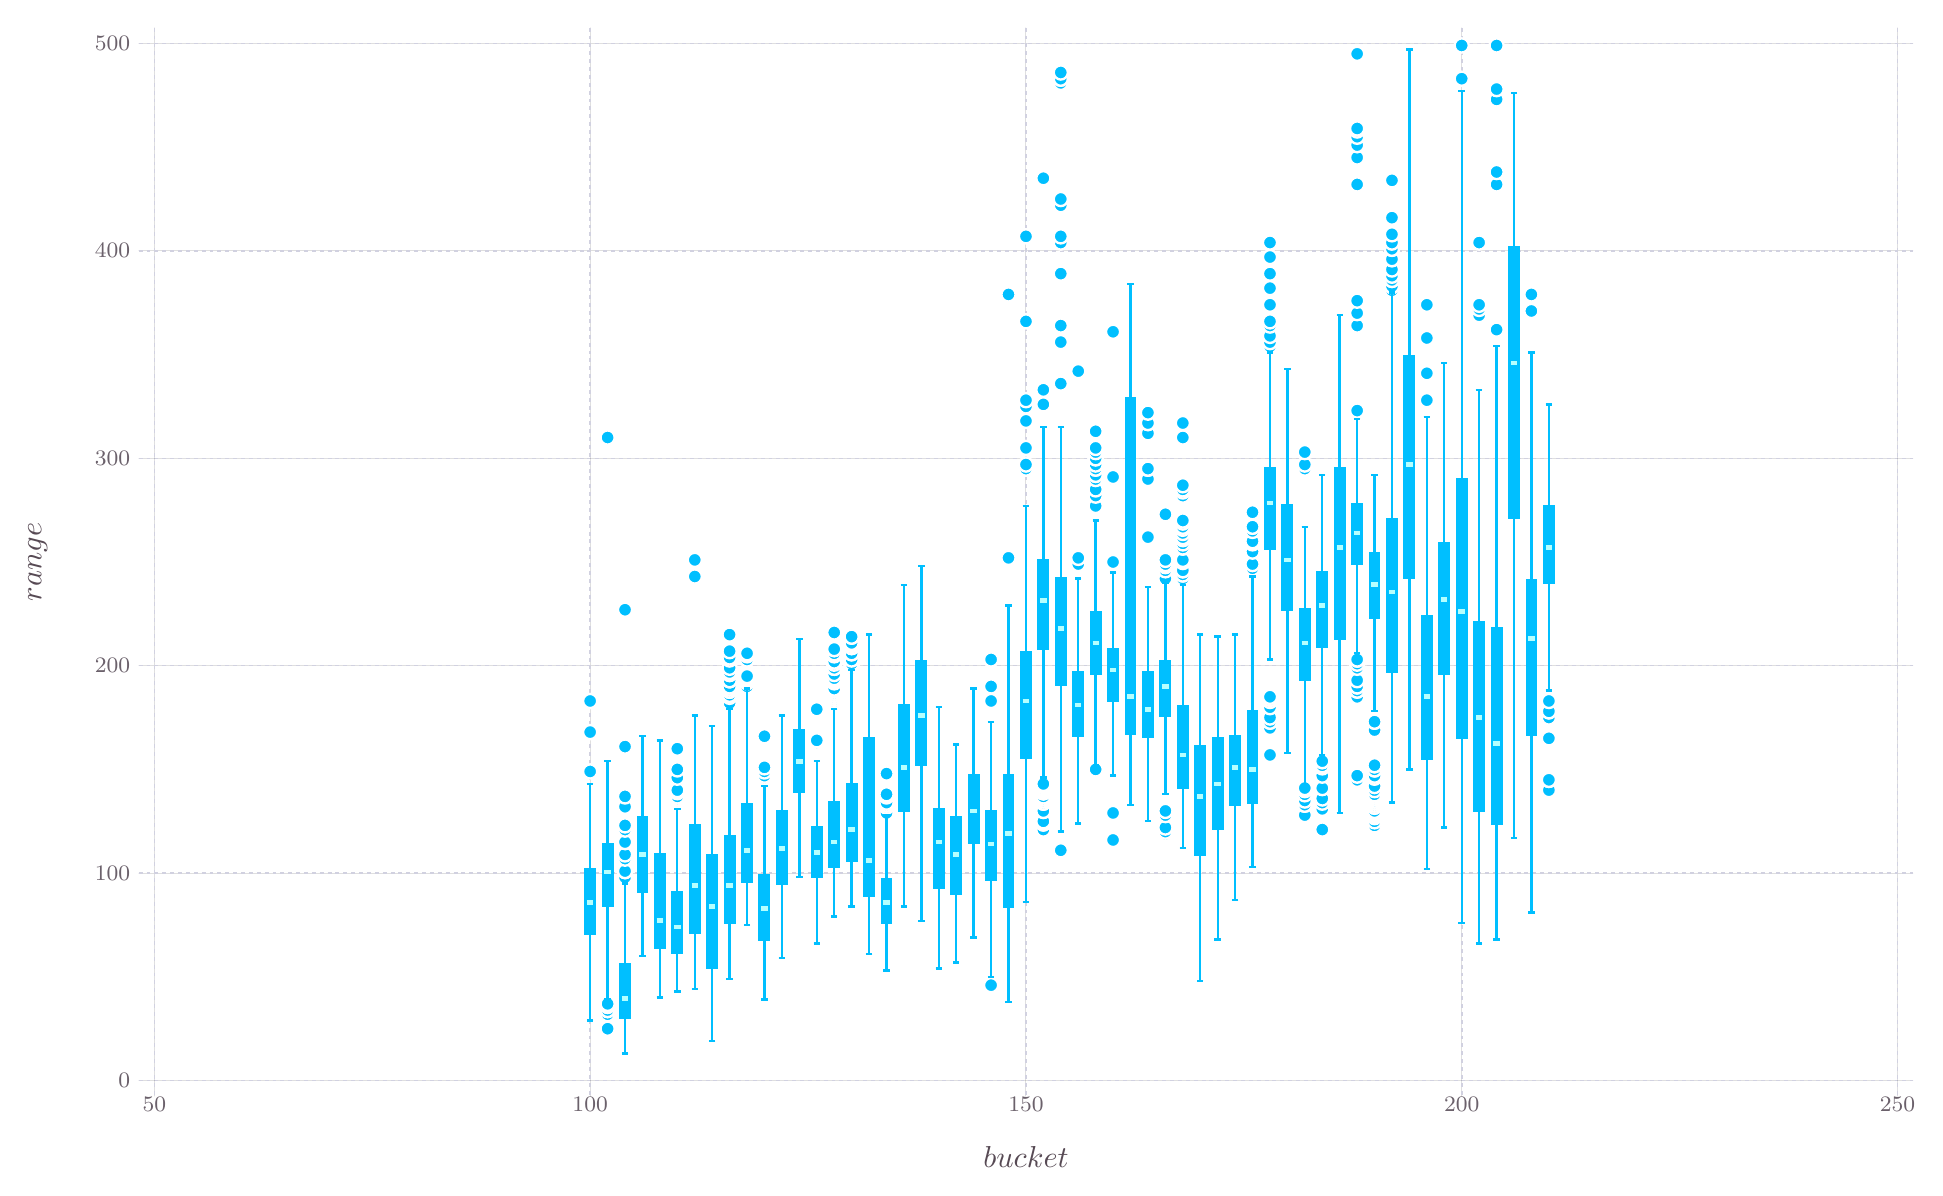
\begin{tikzpicture}[x=1mm,y=-1mm]
\definecolor{mycolor00BFFF}{rgb}{0,0.75,1}
\definecolor{mycolorD0D0E0}{rgb}{0.82,0.82,0.88}
\definecolor{mycolor000000}{rgb}{0,0,0}
\definecolor{mycolor564A55}{rgb}{0.34,0.29,0.33}
\definecolor{mycolor000000}{rgb}{0,0,0}
\definecolor{mycolorFFFFFF}{rgb}{1,1,1}
\definecolor{mycolorB5FFFF}{rgb}{0.71,1,1}
\definecolor{mycolor6C606B}{rgb}{0.42,0.38,0.42}
\begin{scope}
\begin{scope}
\draw (132.32,148.39) node [text=mycolor564A55,draw=mycolor000000,draw opacity=0,rotate around={-0: (0,1.81)},inner sep=0.0]{\fontsize{3.88mm}{4.66mm}\selectfont $\text{bucket}$};
\end{scope}
\begin{scope}
\draw (21.63,141.72) node [text=mycolor6C606B,rotate around={-0: (110.68,1.34)},inner sep=0.0]{\fontsize{2.82mm}{3.39mm}\selectfont $\text{50}$};
\draw (76.97,141.72) node [text=mycolor6C606B,rotate around={-0: (55.34,1.34)},inner sep=0.0]{\fontsize{2.82mm}{3.39mm}\selectfont $\text{100}$};
\draw (132.32,141.72) node [text=mycolor6C606B,rotate around={-0: (-0,1.34)},inner sep=0.0]{\fontsize{2.82mm}{3.39mm}\selectfont $\text{150}$};
\draw (187.66,141.72) node [text=mycolor6C606B,rotate around={-0: (-55.34,1.34)},inner sep=0.0]{\fontsize{2.82mm}{3.39mm}\selectfont $\text{200}$};
\draw (243,141.72) node [text=mycolor6C606B,rotate around={-0: (-110.68,1.34)},inner sep=0.0]{\fontsize{2.82mm}{3.39mm}\selectfont $\text{250}$};
\end{scope}
\begin{scope}
\clip  (19.63,5) -- (245,5) -- (245,140.72) -- (19.63,140.72);
\begin{scope}
\clip  (19.63,5) -- (245,5) -- (245,140.72) -- (19.63,140.72);
\path [fill=mycolor000000,fill opacity=0,draw=mycolor000000,draw opacity=0] (19.63,5) rectangle +(225.37,135.72);
\end{scope}
\begin{scope}
[dash pattern=on 0.5mm off 0.5mm,line width=0.2mm]
\path [fill=mycolor000000,draw=mycolorD0D0E0]  (19.63,138.72) -- (245,138.72);
\path [fill=mycolor000000,draw=mycolorD0D0E0]  (19.63,112.37) -- (245,112.37);
\path [fill=mycolor000000,draw=mycolorD0D0E0]  (19.63,86.03) -- (245,86.03);
\path [fill=mycolor000000,draw=mycolorD0D0E0]  (19.63,59.69) -- (245,59.69);
\path [fill=mycolor000000,draw=mycolorD0D0E0]  (19.63,33.34) -- (245,33.34);
\path [fill=mycolor000000,draw=mycolorD0D0E0]  (19.63,7) -- (245,7);
\end{scope}
\begin{scope}
[dash pattern=on 0.5mm off 0.5mm,line width=0.2mm]
\path [fill=mycolor000000,draw=mycolorD0D0E0]  (21.63,5) -- (21.63,140.72);
\path [fill=mycolor000000,draw=mycolorD0D0E0]  (76.97,5) -- (76.97,140.72);
\path [fill=mycolor000000,draw=mycolorD0D0E0]  (132.32,5) -- (132.32,140.72);
\path [fill=mycolor000000,draw=mycolorD0D0E0]  (187.66,5) -- (187.66,140.72);
\path [fill=mycolor000000,draw=mycolorD0D0E0]  (243,5) -- (243,140.72);
\end{scope}
\begin{scope}
\begin{scope}
[line width=0.3mm]
\path [fill=mycolor00BFFF,draw=mycolorFFFFFF] (76.97,99.46) circle [radius=0.9];
\path [fill=mycolor00BFFF,draw=mycolorFFFFFF] (76.97,94.46) circle [radius=0.9];
\path [fill=mycolor00BFFF,draw=mycolorFFFFFF] (76.97,90.51) circle [radius=0.9];
\path [fill=mycolor00BFFF,draw=mycolorFFFFFF] (79.19,132.13) circle [radius=0.9];
\path [fill=mycolor00BFFF,draw=mycolorFFFFFF] (79.19,130.29) circle [radius=0.9];
\path [fill=mycolor00BFFF,draw=mycolorFFFFFF] (79.19,129.76) circle [radius=0.9];
\path [fill=mycolor00BFFF,draw=mycolorFFFFFF] (79.19,129.76) circle [radius=0.9];
\path [fill=mycolor00BFFF,draw=mycolorFFFFFF] (79.19,129.23) circle [radius=0.9];
\path [fill=mycolor00BFFF,draw=mycolorFFFFFF] (79.19,129.23) circle [radius=0.9];
\path [fill=mycolor00BFFF,draw=mycolorFFFFFF] (79.19,128.97) circle [radius=0.9];
\path [fill=mycolor00BFFF,draw=mycolorFFFFFF] (79.19,128.97) circle [radius=0.9];
\path [fill=mycolor00BFFF,draw=mycolorFFFFFF] (79.19,128.97) circle [radius=0.9];
\path [fill=mycolor00BFFF,draw=mycolorFFFFFF] (79.19,57.05) circle [radius=0.9];
\path [fill=mycolor00BFFF,draw=mycolorFFFFFF] (81.4,112.9) circle [radius=0.9];
\path [fill=mycolor00BFFF,draw=mycolorFFFFFF] (81.4,112.9) circle [radius=0.9];
\path [fill=mycolor00BFFF,draw=mycolorFFFFFF] (81.4,112.9) circle [radius=0.9];
\path [fill=mycolor00BFFF,draw=mycolorFFFFFF] (81.4,112.9) circle [radius=0.9];
\path [fill=mycolor00BFFF,draw=mycolorFFFFFF] (81.4,112.9) circle [radius=0.9];
\path [fill=mycolor00BFFF,draw=mycolorFFFFFF] (81.4,112.11) circle [radius=0.9];
\path [fill=mycolor00BFFF,draw=mycolorFFFFFF] (81.4,112.11) circle [radius=0.9];
\path [fill=mycolor00BFFF,draw=mycolorFFFFFF] (81.4,110.53) circle [radius=0.9];
\path [fill=mycolor00BFFF,draw=mycolorFFFFFF] (81.4,110) circle [radius=0.9];
\path [fill=mycolor00BFFF,draw=mycolorFFFFFF] (81.4,108.42) circle [radius=0.9];
\path [fill=mycolor00BFFF,draw=mycolorFFFFFF] (81.4,108.42) circle [radius=0.9];
\path [fill=mycolor00BFFF,draw=mycolorFFFFFF] (81.4,106.84) circle [radius=0.9];
\path [fill=mycolor00BFFF,draw=mycolorFFFFFF] (81.4,106.31) circle [radius=0.9];
\path [fill=mycolor00BFFF,draw=mycolorFFFFFF] (81.4,103.94) circle [radius=0.9];
\path [fill=mycolor00BFFF,draw=mycolorFFFFFF] (81.4,102.63) circle [radius=0.9];
\path [fill=mycolor00BFFF,draw=mycolorFFFFFF] (81.4,96.3) circle [radius=0.9];
\path [fill=mycolor00BFFF,draw=mycolorFFFFFF] (81.4,78.92) circle [radius=0.9];
\path [fill=mycolor00BFFF,draw=mycolorFFFFFF] (88.04,103.15) circle [radius=0.9];
\path [fill=mycolor00BFFF,draw=mycolorFFFFFF] (88.04,102.89) circle [radius=0.9];
\path [fill=mycolor00BFFF,draw=mycolorFFFFFF] (88.04,102.89) circle [radius=0.9];
\path [fill=mycolor00BFFF,draw=mycolorFFFFFF] (88.04,102.63) circle [radius=0.9];
\path [fill=mycolor00BFFF,draw=mycolorFFFFFF] (88.04,102.1) circle [radius=0.9];
\path [fill=mycolor00BFFF,draw=mycolorFFFFFF] (88.04,101.83) circle [radius=0.9];
\path [fill=mycolor00BFFF,draw=mycolorFFFFFF] (88.04,101.83) circle [radius=0.9];
\path [fill=mycolor00BFFF,draw=mycolorFFFFFF] (88.04,101.83) circle [radius=0.9];
\path [fill=mycolor00BFFF,draw=mycolorFFFFFF] (88.04,100.25) circle [radius=0.9];
\path [fill=mycolor00BFFF,draw=mycolorFFFFFF] (88.04,99.2) circle [radius=0.9];
\path [fill=mycolor00BFFF,draw=mycolorFFFFFF] (88.04,96.57) circle [radius=0.9];
\path [fill=mycolor00BFFF,draw=mycolorFFFFFF] (90.26,74.7) circle [radius=0.9];
\path [fill=mycolor00BFFF,draw=mycolorFFFFFF] (90.26,72.59) circle [radius=0.9];
\path [fill=mycolor00BFFF,draw=mycolorFFFFFF] (94.68,90.77) circle [radius=0.9];
\path [fill=mycolor00BFFF,draw=mycolorFFFFFF] (94.68,90.77) circle [radius=0.9];
\path [fill=mycolor00BFFF,draw=mycolorFFFFFF] (94.68,90.77) circle [radius=0.9];
\path [fill=mycolor00BFFF,draw=mycolorFFFFFF] (94.68,89.98) circle [radius=0.9];
\path [fill=mycolor00BFFF,draw=mycolorFFFFFF] (94.68,89.72) circle [radius=0.9];
\path [fill=mycolor00BFFF,draw=mycolorFFFFFF] (94.68,89.72) circle [radius=0.9];
\path [fill=mycolor00BFFF,draw=mycolorFFFFFF] (94.68,89.72) circle [radius=0.9];
\path [fill=mycolor00BFFF,draw=mycolorFFFFFF] (94.68,89.19) circle [radius=0.9];
\path [fill=mycolor00BFFF,draw=mycolorFFFFFF] (94.68,89.19) circle [radius=0.9];
\path [fill=mycolor00BFFF,draw=mycolorFFFFFF] (94.68,89.19) circle [radius=0.9];
\path [fill=mycolor00BFFF,draw=mycolorFFFFFF] (94.68,89.19) circle [radius=0.9];
\path [fill=mycolor00BFFF,draw=mycolorFFFFFF] (94.68,88.93) circle [radius=0.9];
\path [fill=mycolor00BFFF,draw=mycolorFFFFFF] (94.68,88.66) circle [radius=0.9];
\path [fill=mycolor00BFFF,draw=mycolorFFFFFF] (94.68,88.66) circle [radius=0.9];
\path [fill=mycolor00BFFF,draw=mycolorFFFFFF] (94.68,87.87) circle [radius=0.9];
\path [fill=mycolor00BFFF,draw=mycolorFFFFFF] (94.68,87.87) circle [radius=0.9];
\path [fill=mycolor00BFFF,draw=mycolorFFFFFF] (94.68,87.87) circle [radius=0.9];
\path [fill=mycolor00BFFF,draw=mycolorFFFFFF] (94.68,87.08) circle [radius=0.9];
\path [fill=mycolor00BFFF,draw=mycolorFFFFFF] (94.68,87.08) circle [radius=0.9];
\path [fill=mycolor00BFFF,draw=mycolorFFFFFF] (94.68,86.82) circle [radius=0.9];
\path [fill=mycolor00BFFF,draw=mycolorFFFFFF] (94.68,86.29) circle [radius=0.9];
\path [fill=mycolor00BFFF,draw=mycolorFFFFFF] (94.68,85.24) circle [radius=0.9];
\path [fill=mycolor00BFFF,draw=mycolorFFFFFF] (94.68,84.98) circle [radius=0.9];
\path [fill=mycolor00BFFF,draw=mycolorFFFFFF] (94.68,84.18) circle [radius=0.9];
\path [fill=mycolor00BFFF,draw=mycolorFFFFFF] (94.68,82.08) circle [radius=0.9];
\path [fill=mycolor00BFFF,draw=mycolorFFFFFF] (96.9,88.66) circle [radius=0.9];
\path [fill=mycolor00BFFF,draw=mycolorFFFFFF] (96.9,88.14) circle [radius=0.9];
\path [fill=mycolor00BFFF,draw=mycolorFFFFFF] (96.9,87.87) circle [radius=0.9];
\path [fill=mycolor00BFFF,draw=mycolorFFFFFF] (96.9,87.61) circle [radius=0.9];
\path [fill=mycolor00BFFF,draw=mycolorFFFFFF] (96.9,87.35) circle [radius=0.9];
\path [fill=mycolor00BFFF,draw=mycolorFFFFFF] (96.9,85.24) circle [radius=0.9];
\path [fill=mycolor00BFFF,draw=mycolorFFFFFF] (96.9,84.71) circle [radius=0.9];
\path [fill=mycolor00BFFF,draw=mycolorFFFFFF] (96.9,84.45) circle [radius=0.9];
\path [fill=mycolor00BFFF,draw=mycolorFFFFFF] (99.11,100.25) circle [radius=0.9];
\path [fill=mycolor00BFFF,draw=mycolorFFFFFF] (99.11,99.99) circle [radius=0.9];
\path [fill=mycolor00BFFF,draw=mycolorFFFFFF] (99.11,99.46) circle [radius=0.9];
\path [fill=mycolor00BFFF,draw=mycolorFFFFFF] (99.11,98.94) circle [radius=0.9];
\path [fill=mycolor00BFFF,draw=mycolorFFFFFF] (99.11,94.99) circle [radius=0.9];
\path [fill=mycolor00BFFF,draw=mycolorFFFFFF] (105.75,95.78) circle [radius=0.9];
\path [fill=mycolor00BFFF,draw=mycolorFFFFFF] (105.75,95.51) circle [radius=0.9];
\path [fill=mycolor00BFFF,draw=mycolorFFFFFF] (105.75,91.56) circle [radius=0.9];
\path [fill=mycolor00BFFF,draw=mycolorFFFFFF] (107.97,90.77) circle [radius=0.9];
\path [fill=mycolor00BFFF,draw=mycolorFFFFFF] (107.97,90.77) circle [radius=0.9];
\path [fill=mycolor00BFFF,draw=mycolorFFFFFF] (107.97,90.77) circle [radius=0.9];
\path [fill=mycolor00BFFF,draw=mycolorFFFFFF] (107.97,90.51) circle [radius=0.9];
\path [fill=mycolor00BFFF,draw=mycolorFFFFFF] (107.97,90.24) circle [radius=0.9];
\path [fill=mycolor00BFFF,draw=mycolorFFFFFF] (107.97,89.98) circle [radius=0.9];
\path [fill=mycolor00BFFF,draw=mycolorFFFFFF] (107.97,89.72) circle [radius=0.9];
\path [fill=mycolor00BFFF,draw=mycolorFFFFFF] (107.97,89.45) circle [radius=0.9];
\path [fill=mycolor00BFFF,draw=mycolorFFFFFF] (107.97,89.45) circle [radius=0.9];
\path [fill=mycolor00BFFF,draw=mycolorFFFFFF] (107.97,89.19) circle [radius=0.9];
\path [fill=mycolor00BFFF,draw=mycolorFFFFFF] (107.97,88.93) circle [radius=0.9];
\path [fill=mycolor00BFFF,draw=mycolorFFFFFF] (107.97,88.93) circle [radius=0.9];
\path [fill=mycolor00BFFF,draw=mycolorFFFFFF] (107.97,88.14) circle [radius=0.9];
\path [fill=mycolor00BFFF,draw=mycolorFFFFFF] (107.97,87.87) circle [radius=0.9];
\path [fill=mycolor00BFFF,draw=mycolorFFFFFF] (107.97,87.87) circle [radius=0.9];
\path [fill=mycolor00BFFF,draw=mycolorFFFFFF] (107.97,87.87) circle [radius=0.9];
\path [fill=mycolor00BFFF,draw=mycolorFFFFFF] (107.97,87.61) circle [radius=0.9];
\path [fill=mycolor00BFFF,draw=mycolorFFFFFF] (107.97,87.08) circle [radius=0.9];
\path [fill=mycolor00BFFF,draw=mycolorFFFFFF] (107.97,86.29) circle [radius=0.9];
\path [fill=mycolor00BFFF,draw=mycolorFFFFFF] (107.97,86.29) circle [radius=0.9];
\path [fill=mycolor00BFFF,draw=mycolorFFFFFF] (107.97,86.29) circle [radius=0.9];
\path [fill=mycolor00BFFF,draw=mycolorFFFFFF] (107.97,85.77) circle [radius=0.9];
\path [fill=mycolor00BFFF,draw=mycolorFFFFFF] (107.97,85.5) circle [radius=0.9];
\path [fill=mycolor00BFFF,draw=mycolorFFFFFF] (107.97,84.71) circle [radius=0.9];
\path [fill=mycolor00BFFF,draw=mycolorFFFFFF] (107.97,84.45) circle [radius=0.9];
\path [fill=mycolor00BFFF,draw=mycolorFFFFFF] (107.97,83.92) circle [radius=0.9];
\path [fill=mycolor00BFFF,draw=mycolorFFFFFF] (107.97,83.92) circle [radius=0.9];
\path [fill=mycolor00BFFF,draw=mycolorFFFFFF] (107.97,81.81) circle [radius=0.9];
\path [fill=mycolor00BFFF,draw=mycolorFFFFFF] (110.18,86.29) circle [radius=0.9];
\path [fill=mycolor00BFFF,draw=mycolorFFFFFF] (110.18,86.03) circle [radius=0.9];
\path [fill=mycolor00BFFF,draw=mycolorFFFFFF] (110.18,85.77) circle [radius=0.9];
\path [fill=mycolor00BFFF,draw=mycolorFFFFFF] (110.18,85.77) circle [radius=0.9];
\path [fill=mycolor00BFFF,draw=mycolorFFFFFF] (110.18,85.24) circle [radius=0.9];
\path [fill=mycolor00BFFF,draw=mycolorFFFFFF] (110.18,84.45) circle [radius=0.9];
\path [fill=mycolor00BFFF,draw=mycolorFFFFFF] (110.18,84.45) circle [radius=0.9];
\path [fill=mycolor00BFFF,draw=mycolorFFFFFF] (110.18,83.66) circle [radius=0.9];
\path [fill=mycolor00BFFF,draw=mycolorFFFFFF] (110.18,83.66) circle [radius=0.9];
\path [fill=mycolor00BFFF,draw=mycolorFFFFFF] (110.18,83.39) circle [radius=0.9];
\path [fill=mycolor00BFFF,draw=mycolorFFFFFF] (110.18,83.13) circle [radius=0.9];
\path [fill=mycolor00BFFF,draw=mycolorFFFFFF] (110.18,83.13) circle [radius=0.9];
\path [fill=mycolor00BFFF,draw=mycolorFFFFFF] (110.18,83.13) circle [radius=0.9];
\path [fill=mycolor00BFFF,draw=mycolorFFFFFF] (110.18,82.34) circle [radius=0.9];
\path [fill=mycolor00BFFF,draw=mycolorFFFFFF] (110.18,82.34) circle [radius=0.9];
\path [fill=mycolor00BFFF,draw=mycolorFFFFFF] (114.61,104.73) circle [radius=0.9];
\path [fill=mycolor00BFFF,draw=mycolorFFFFFF] (114.61,104.73) circle [radius=0.9];
\path [fill=mycolor00BFFF,draw=mycolorFFFFFF] (114.61,103.94) circle [radius=0.9];
\path [fill=mycolor00BFFF,draw=mycolorFFFFFF] (114.61,103.68) circle [radius=0.9];
\path [fill=mycolor00BFFF,draw=mycolorFFFFFF] (114.61,103.42) circle [radius=0.9];
\path [fill=mycolor00BFFF,draw=mycolorFFFFFF] (114.61,102.63) circle [radius=0.9];
\path [fill=mycolor00BFFF,draw=mycolorFFFFFF] (114.61,102.36) circle [radius=0.9];
\path [fill=mycolor00BFFF,draw=mycolorFFFFFF] (114.61,102.36) circle [radius=0.9];
\path [fill=mycolor00BFFF,draw=mycolorFFFFFF] (114.61,102.36) circle [radius=0.9];
\path [fill=mycolor00BFFF,draw=mycolorFFFFFF] (114.61,99.73) circle [radius=0.9];
\path [fill=mycolor00BFFF,draw=mycolorFFFFFF] (127.89,126.6) circle [radius=0.9];
\path [fill=mycolor00BFFF,draw=mycolorFFFFFF] (127.89,90.51) circle [radius=0.9];
\path [fill=mycolor00BFFF,draw=mycolorFFFFFF] (127.89,88.66) circle [radius=0.9];
\path [fill=mycolor00BFFF,draw=mycolorFFFFFF] (127.89,88.66) circle [radius=0.9];
\path [fill=mycolor00BFFF,draw=mycolorFFFFFF] (127.89,85.24) circle [radius=0.9];
\path [fill=mycolor00BFFF,draw=mycolorFFFFFF] (130.1,72.33) circle [radius=0.9];
\path [fill=mycolor00BFFF,draw=mycolorFFFFFF] (130.1,38.88) circle [radius=0.9];
\path [fill=mycolor00BFFF,draw=mycolorFFFFFF] (132.32,61) circle [radius=0.9];
\path [fill=mycolor00BFFF,draw=mycolorFFFFFF] (132.32,60.48) circle [radius=0.9];
\path [fill=mycolor00BFFF,draw=mycolorFFFFFF] (132.32,58.37) circle [radius=0.9];
\path [fill=mycolor00BFFF,draw=mycolorFFFFFF] (132.32,54.94) circle [radius=0.9];
\path [fill=mycolor00BFFF,draw=mycolorFFFFFF] (132.32,53.1) circle [radius=0.9];
\path [fill=mycolor00BFFF,draw=mycolorFFFFFF] (132.32,52.31) circle [radius=0.9];
\path [fill=mycolor00BFFF,draw=mycolorFFFFFF] (132.32,42.3) circle [radius=0.9];
\path [fill=mycolor00BFFF,draw=mycolorFFFFFF] (132.32,31.5) circle [radius=0.9];
\path [fill=mycolor00BFFF,draw=mycolorFFFFFF] (134.53,106.84) circle [radius=0.9];
\path [fill=mycolor00BFFF,draw=mycolorFFFFFF] (134.53,106.84) circle [radius=0.9];
\path [fill=mycolor00BFFF,draw=mycolorFFFFFF] (134.53,106.84) circle [radius=0.9];
\path [fill=mycolor00BFFF,draw=mycolorFFFFFF] (134.53,106.05) circle [radius=0.9];
\path [fill=mycolor00BFFF,draw=mycolorFFFFFF] (134.53,106.05) circle [radius=0.9];
\path [fill=mycolor00BFFF,draw=mycolorFFFFFF] (134.53,106.05) circle [radius=0.9];
\path [fill=mycolor00BFFF,draw=mycolorFFFFFF] (134.53,105.79) circle [radius=0.9];
\path [fill=mycolor00BFFF,draw=mycolorFFFFFF] (134.53,104.47) circle [radius=0.9];
\path [fill=mycolor00BFFF,draw=mycolorFFFFFF] (134.53,104.47) circle [radius=0.9];
\path [fill=mycolor00BFFF,draw=mycolorFFFFFF] (134.53,103.42) circle [radius=0.9];
\path [fill=mycolor00BFFF,draw=mycolorFFFFFF] (134.53,103.42) circle [radius=0.9];
\path [fill=mycolor00BFFF,draw=mycolorFFFFFF] (134.53,103.15) circle [radius=0.9];
\path [fill=mycolor00BFFF,draw=mycolorFFFFFF] (134.53,102.89) circle [radius=0.9];
\path [fill=mycolor00BFFF,draw=mycolorFFFFFF] (134.53,102.63) circle [radius=0.9];
\path [fill=mycolor00BFFF,draw=mycolorFFFFFF] (134.53,102.1) circle [radius=0.9];
\path [fill=mycolor00BFFF,draw=mycolorFFFFFF] (134.53,102.1) circle [radius=0.9];
\path [fill=mycolor00BFFF,draw=mycolorFFFFFF] (134.53,102.1) circle [radius=0.9];
\path [fill=mycolor00BFFF,draw=mycolorFFFFFF] (134.53,101.83) circle [radius=0.9];
\path [fill=mycolor00BFFF,draw=mycolorFFFFFF] (134.53,101.83) circle [radius=0.9];
\path [fill=mycolor00BFFF,draw=mycolorFFFFFF] (134.53,101.57) circle [radius=0.9];
\path [fill=mycolor00BFFF,draw=mycolorFFFFFF] (134.53,101.57) circle [radius=0.9];
\path [fill=mycolor00BFFF,draw=mycolorFFFFFF] (134.53,101.57) circle [radius=0.9];
\path [fill=mycolor00BFFF,draw=mycolorFFFFFF] (134.53,101.31) circle [radius=0.9];
\path [fill=mycolor00BFFF,draw=mycolorFFFFFF] (134.53,101.04) circle [radius=0.9];
\path [fill=mycolor00BFFF,draw=mycolorFFFFFF] (134.53,101.04) circle [radius=0.9];
\path [fill=mycolor00BFFF,draw=mycolorFFFFFF] (134.53,52.84) circle [radius=0.9];
\path [fill=mycolor00BFFF,draw=mycolorFFFFFF] (134.53,50.99) circle [radius=0.9];
\path [fill=mycolor00BFFF,draw=mycolorFFFFFF] (134.53,24.12) circle [radius=0.9];
\path [fill=mycolor00BFFF,draw=mycolorFFFFFF] (136.74,109.47) circle [radius=0.9];
\path [fill=mycolor00BFFF,draw=mycolorFFFFFF] (136.74,50.2) circle [radius=0.9];
\path [fill=mycolor00BFFF,draw=mycolorFFFFFF] (136.74,44.93) circle [radius=0.9];
\path [fill=mycolor00BFFF,draw=mycolorFFFFFF] (136.74,42.83) circle [radius=0.9];
\path [fill=mycolor00BFFF,draw=mycolorFFFFFF] (136.74,36.24) circle [radius=0.9];
\path [fill=mycolor00BFFF,draw=mycolorFFFFFF] (136.74,32.29) circle [radius=0.9];
\path [fill=mycolor00BFFF,draw=mycolorFFFFFF] (136.74,31.5) circle [radius=0.9];
\path [fill=mycolor00BFFF,draw=mycolorFFFFFF] (136.74,27.55) circle [radius=0.9];
\path [fill=mycolor00BFFF,draw=mycolorFFFFFF] (136.74,26.76) circle [radius=0.9];
\path [fill=mycolor00BFFF,draw=mycolorFFFFFF] (136.74,12.01) circle [radius=0.9];
\path [fill=mycolor00BFFF,draw=mycolorFFFFFF] (136.74,11.48) circle [radius=0.9];
\path [fill=mycolor00BFFF,draw=mycolorFFFFFF] (136.74,11.48) circle [radius=0.9];
\path [fill=mycolor00BFFF,draw=mycolorFFFFFF] (136.74,10.69) circle [radius=0.9];
\path [fill=mycolor00BFFF,draw=mycolorFFFFFF] (138.96,73.12) circle [radius=0.9];
\path [fill=mycolor00BFFF,draw=mycolorFFFFFF] (138.96,73.12) circle [radius=0.9];
\path [fill=mycolor00BFFF,draw=mycolorFFFFFF] (138.96,72.33) circle [radius=0.9];
\path [fill=mycolor00BFFF,draw=mycolorFFFFFF] (138.96,48.62) circle [radius=0.9];
\path [fill=mycolor00BFFF,draw=mycolorFFFFFF] (141.17,99.2) circle [radius=0.9];
\path [fill=mycolor00BFFF,draw=mycolorFFFFFF] (141.17,65.74) circle [radius=0.9];
\path [fill=mycolor00BFFF,draw=mycolorFFFFFF] (141.17,65.74) circle [radius=0.9];
\path [fill=mycolor00BFFF,draw=mycolorFFFFFF] (141.17,65.74) circle [radius=0.9];
\path [fill=mycolor00BFFF,draw=mycolorFFFFFF] (141.17,64.43) circle [radius=0.9];
\path [fill=mycolor00BFFF,draw=mycolorFFFFFF] (141.17,63.64) circle [radius=0.9];
\path [fill=mycolor00BFFF,draw=mycolorFFFFFF] (141.17,62.32) circle [radius=0.9];
\path [fill=mycolor00BFFF,draw=mycolorFFFFFF] (141.17,61.79) circle [radius=0.9];
\path [fill=mycolor00BFFF,draw=mycolorFFFFFF] (141.17,61.79) circle [radius=0.9];
\path [fill=mycolor00BFFF,draw=mycolorFFFFFF] (141.17,61) circle [radius=0.9];
\path [fill=mycolor00BFFF,draw=mycolorFFFFFF] (141.17,61) circle [radius=0.9];
\path [fill=mycolor00BFFF,draw=mycolorFFFFFF] (141.17,60.48) circle [radius=0.9];
\path [fill=mycolor00BFFF,draw=mycolorFFFFFF] (141.17,59.69) circle [radius=0.9];
\path [fill=mycolor00BFFF,draw=mycolorFFFFFF] (141.17,59.69) circle [radius=0.9];
\path [fill=mycolor00BFFF,draw=mycolorFFFFFF] (141.17,58.9) circle [radius=0.9];
\path [fill=mycolor00BFFF,draw=mycolorFFFFFF] (141.17,58.37) circle [radius=0.9];
\path [fill=mycolor00BFFF,draw=mycolorFFFFFF] (141.17,56.26) circle [radius=0.9];
\path [fill=mycolor00BFFF,draw=mycolorFFFFFF] (141.17,56.26) circle [radius=0.9];
\path [fill=mycolor00BFFF,draw=mycolorFFFFFF] (143.38,108.16) circle [radius=0.9];
\path [fill=mycolor00BFFF,draw=mycolorFFFFFF] (143.38,104.73) circle [radius=0.9];
\path [fill=mycolor00BFFF,draw=mycolorFFFFFF] (143.38,72.86) circle [radius=0.9];
\path [fill=mycolor00BFFF,draw=mycolorFFFFFF] (143.38,62.32) circle [radius=0.9];
\path [fill=mycolor00BFFF,draw=mycolorFFFFFF] (143.38,62.06) circle [radius=0.9];
\path [fill=mycolor00BFFF,draw=mycolorFFFFFF] (143.38,43.62) circle [radius=0.9];
\path [fill=mycolor00BFFF,draw=mycolorFFFFFF] (147.81,69.7) circle [radius=0.9];
\path [fill=mycolor00BFFF,draw=mycolorFFFFFF] (147.81,62.32) circle [radius=0.9];
\path [fill=mycolor00BFFF,draw=mycolorFFFFFF] (147.81,61) circle [radius=0.9];
\path [fill=mycolor00BFFF,draw=mycolorFFFFFF] (147.81,61) circle [radius=0.9];
\path [fill=mycolor00BFFF,draw=mycolorFFFFFF] (147.81,61) circle [radius=0.9];
\path [fill=mycolor00BFFF,draw=mycolorFFFFFF] (147.81,56.52) circle [radius=0.9];
\path [fill=mycolor00BFFF,draw=mycolorFFFFFF] (147.81,55.21) circle [radius=0.9];
\path [fill=mycolor00BFFF,draw=mycolorFFFFFF] (147.81,55.21) circle [radius=0.9];
\path [fill=mycolor00BFFF,draw=mycolorFFFFFF] (147.81,53.89) circle [radius=0.9];
\path [fill=mycolor00BFFF,draw=mycolorFFFFFF] (150.03,107.37) circle [radius=0.9];
\path [fill=mycolor00BFFF,draw=mycolorFFFFFF] (150.03,107.1) circle [radius=0.9];
\path [fill=mycolor00BFFF,draw=mycolorFFFFFF] (150.03,106.58) circle [radius=0.9];
\path [fill=mycolor00BFFF,draw=mycolorFFFFFF] (150.03,105) circle [radius=0.9];
\path [fill=mycolor00BFFF,draw=mycolorFFFFFF] (150.03,104.47) circle [radius=0.9];
\path [fill=mycolor00BFFF,draw=mycolorFFFFFF] (150.03,74.96) circle [radius=0.9];
\path [fill=mycolor00BFFF,draw=mycolorFFFFFF] (150.03,73.91) circle [radius=0.9];
\path [fill=mycolor00BFFF,draw=mycolorFFFFFF] (150.03,73.38) circle [radius=0.9];
\path [fill=mycolor00BFFF,draw=mycolorFFFFFF] (150.03,73.12) circle [radius=0.9];
\path [fill=mycolor00BFFF,draw=mycolorFFFFFF] (150.03,72.59) circle [radius=0.9];
\path [fill=mycolor00BFFF,draw=mycolorFFFFFF] (150.03,66.8) circle [radius=0.9];
\path [fill=mycolor00BFFF,draw=mycolorFFFFFF] (152.24,74.96) circle [radius=0.9];
\path [fill=mycolor00BFFF,draw=mycolorFFFFFF] (152.24,74.44) circle [radius=0.9];
\path [fill=mycolor00BFFF,draw=mycolorFFFFFF] (152.24,74.44) circle [radius=0.9];
\path [fill=mycolor00BFFF,draw=mycolorFFFFFF] (152.24,73.91) circle [radius=0.9];
\path [fill=mycolor00BFFF,draw=mycolorFFFFFF] (152.24,73.91) circle [radius=0.9];
\path [fill=mycolor00BFFF,draw=mycolorFFFFFF] (152.24,72.86) circle [radius=0.9];
\path [fill=mycolor00BFFF,draw=mycolorFFFFFF] (152.24,72.59) circle [radius=0.9];
\path [fill=mycolor00BFFF,draw=mycolorFFFFFF] (152.24,72.59) circle [radius=0.9];
\path [fill=mycolor00BFFF,draw=mycolorFFFFFF] (152.24,71.01) circle [radius=0.9];
\path [fill=mycolor00BFFF,draw=mycolorFFFFFF] (152.24,71.01) circle [radius=0.9];
\path [fill=mycolor00BFFF,draw=mycolorFFFFFF] (152.24,71.01) circle [radius=0.9];
\path [fill=mycolor00BFFF,draw=mycolorFFFFFF] (152.24,70.49) circle [radius=0.9];
\path [fill=mycolor00BFFF,draw=mycolorFFFFFF] (152.24,69.96) circle [radius=0.9];
\path [fill=mycolor00BFFF,draw=mycolorFFFFFF] (152.24,69.7) circle [radius=0.9];
\path [fill=mycolor00BFFF,draw=mycolorFFFFFF] (152.24,69.17) circle [radius=0.9];
\path [fill=mycolor00BFFF,draw=mycolorFFFFFF] (152.24,68.64) circle [radius=0.9];
\path [fill=mycolor00BFFF,draw=mycolorFFFFFF] (152.24,68.38) circle [radius=0.9];
\path [fill=mycolor00BFFF,draw=mycolorFFFFFF] (152.24,67.85) circle [radius=0.9];
\path [fill=mycolor00BFFF,draw=mycolorFFFFFF] (152.24,67.59) circle [radius=0.9];
\path [fill=mycolor00BFFF,draw=mycolorFFFFFF] (152.24,64.43) circle [radius=0.9];
\path [fill=mycolor00BFFF,draw=mycolorFFFFFF] (152.24,63.9) circle [radius=0.9];
\path [fill=mycolor00BFFF,draw=mycolorFFFFFF] (152.24,63.64) circle [radius=0.9];
\path [fill=mycolor00BFFF,draw=mycolorFFFFFF] (152.24,63.11) circle [radius=0.9];
\path [fill=mycolor00BFFF,draw=mycolorFFFFFF] (152.24,57.05) circle [radius=0.9];
\path [fill=mycolor00BFFF,draw=mycolorFFFFFF] (152.24,55.21) circle [radius=0.9];
\path [fill=mycolor00BFFF,draw=mycolorFFFFFF] (152.24,55.21) circle [radius=0.9];
\path [fill=mycolor00BFFF,draw=mycolorFFFFFF] (161.09,73.91) circle [radius=0.9];
\path [fill=mycolor00BFFF,draw=mycolorFFFFFF] (161.09,73.65) circle [radius=0.9];
\path [fill=mycolor00BFFF,draw=mycolorFFFFFF] (161.09,73.65) circle [radius=0.9];
\path [fill=mycolor00BFFF,draw=mycolorFFFFFF] (161.09,73.12) circle [radius=0.9];
\path [fill=mycolor00BFFF,draw=mycolorFFFFFF] (161.09,71.54) circle [radius=0.9];
\path [fill=mycolor00BFFF,draw=mycolorFFFFFF] (161.09,70.49) circle [radius=0.9];
\path [fill=mycolor00BFFF,draw=mycolorFFFFFF] (161.09,70.22) circle [radius=0.9];
\path [fill=mycolor00BFFF,draw=mycolorFFFFFF] (161.09,68.91) circle [radius=0.9];
\path [fill=mycolor00BFFF,draw=mycolorFFFFFF] (161.09,68.38) circle [radius=0.9];
\path [fill=mycolor00BFFF,draw=mycolorFFFFFF] (161.09,68.38) circle [radius=0.9];
\path [fill=mycolor00BFFF,draw=mycolorFFFFFF] (161.09,66.54) circle [radius=0.9];
\path [fill=mycolor00BFFF,draw=mycolorFFFFFF] (161.09,66.54) circle [radius=0.9];
\path [fill=mycolor00BFFF,draw=mycolorFFFFFF] (163.31,97.36) circle [radius=0.9];
\path [fill=mycolor00BFFF,draw=mycolorFFFFFF] (163.31,93.93) circle [radius=0.9];
\path [fill=mycolor00BFFF,draw=mycolorFFFFFF] (163.31,93.93) circle [radius=0.9];
\path [fill=mycolor00BFFF,draw=mycolorFFFFFF] (163.31,93.93) circle [radius=0.9];
\path [fill=mycolor00BFFF,draw=mycolorFFFFFF] (163.31,93.14) circle [radius=0.9];
\path [fill=mycolor00BFFF,draw=mycolorFFFFFF] (163.31,93.14) circle [radius=0.9];
\path [fill=mycolor00BFFF,draw=mycolorFFFFFF] (163.31,92.61) circle [radius=0.9];
\path [fill=mycolor00BFFF,draw=mycolorFFFFFF] (163.31,91.3) circle [radius=0.9];
\path [fill=mycolor00BFFF,draw=mycolorFFFFFF] (163.31,90.51) circle [radius=0.9];
\path [fill=mycolor00BFFF,draw=mycolorFFFFFF] (163.31,90.24) circle [radius=0.9];
\path [fill=mycolor00BFFF,draw=mycolorFFFFFF] (163.31,89.98) circle [radius=0.9];
\path [fill=mycolor00BFFF,draw=mycolorFFFFFF] (163.31,45.46) circle [radius=0.9];
\path [fill=mycolor00BFFF,draw=mycolorFFFFFF] (163.31,45.46) circle [radius=0.9];
\path [fill=mycolor00BFFF,draw=mycolorFFFFFF] (163.31,44.93) circle [radius=0.9];
\path [fill=mycolor00BFFF,draw=mycolorFFFFFF] (163.31,44.14) circle [radius=0.9];
\path [fill=mycolor00BFFF,draw=mycolorFFFFFF] (163.31,42.83) circle [radius=0.9];
\path [fill=mycolor00BFFF,draw=mycolorFFFFFF] (163.31,42.3) circle [radius=0.9];
\path [fill=mycolor00BFFF,draw=mycolorFFFFFF] (163.31,40.19) circle [radius=0.9];
\path [fill=mycolor00BFFF,draw=mycolorFFFFFF] (163.31,40.19) circle [radius=0.9];
\path [fill=mycolor00BFFF,draw=mycolorFFFFFF] (163.31,38.08) circle [radius=0.9];
\path [fill=mycolor00BFFF,draw=mycolorFFFFFF] (163.31,38.08) circle [radius=0.9];
\path [fill=mycolor00BFFF,draw=mycolorFFFFFF] (163.31,36.24) circle [radius=0.9];
\path [fill=mycolor00BFFF,draw=mycolorFFFFFF] (163.31,34.13) circle [radius=0.9];
\path [fill=mycolor00BFFF,draw=mycolorFFFFFF] (163.31,32.29) circle [radius=0.9];
\path [fill=mycolor00BFFF,draw=mycolorFFFFFF] (167.73,105) circle [radius=0.9];
\path [fill=mycolor00BFFF,draw=mycolorFFFFFF] (167.73,103.68) circle [radius=0.9];
\path [fill=mycolor00BFFF,draw=mycolorFFFFFF] (167.73,103.68) circle [radius=0.9];
\path [fill=mycolor00BFFF,draw=mycolorFFFFFF] (167.73,103.15) circle [radius=0.9];
\path [fill=mycolor00BFFF,draw=mycolorFFFFFF] (167.73,102.36) circle [radius=0.9];
\path [fill=mycolor00BFFF,draw=mycolorFFFFFF] (167.73,101.83) circle [radius=0.9];
\path [fill=mycolor00BFFF,draw=mycolorFFFFFF] (167.73,101.57) circle [radius=0.9];
\path [fill=mycolor00BFFF,draw=mycolorFFFFFF] (167.73,61) circle [radius=0.9];
\path [fill=mycolor00BFFF,draw=mycolorFFFFFF] (167.73,60.48) circle [radius=0.9];
\path [fill=mycolor00BFFF,draw=mycolorFFFFFF] (167.73,58.9) circle [radius=0.9];
\path [fill=mycolor00BFFF,draw=mycolorFFFFFF] (169.95,106.84) circle [radius=0.9];
\path [fill=mycolor00BFFF,draw=mycolorFFFFFF] (169.95,104.21) circle [radius=0.9];
\path [fill=mycolor00BFFF,draw=mycolorFFFFFF] (169.95,103.42) circle [radius=0.9];
\path [fill=mycolor00BFFF,draw=mycolorFFFFFF] (169.95,102.89) circle [radius=0.9];
\path [fill=mycolor00BFFF,draw=mycolorFFFFFF] (169.95,101.57) circle [radius=0.9];
\path [fill=mycolor00BFFF,draw=mycolorFFFFFF] (169.95,99.99) circle [radius=0.9];
\path [fill=mycolor00BFFF,draw=mycolorFFFFFF] (169.95,98.94) circle [radius=0.9];
\path [fill=mycolor00BFFF,draw=mycolorFFFFFF] (169.95,98.67) circle [radius=0.9];
\path [fill=mycolor00BFFF,draw=mycolorFFFFFF] (169.95,98.15) circle [radius=0.9];
\path [fill=mycolor00BFFF,draw=mycolorFFFFFF] (169.95,98.15) circle [radius=0.9];
\path [fill=mycolor00BFFF,draw=mycolorFFFFFF] (174.38,100.78) circle [radius=0.9];
\path [fill=mycolor00BFFF,draw=mycolorFFFFFF] (174.38,100.52) circle [radius=0.9];
\path [fill=mycolor00BFFF,draw=mycolorFFFFFF] (174.38,100.52) circle [radius=0.9];
\path [fill=mycolor00BFFF,draw=mycolorFFFFFF] (174.38,99.99) circle [radius=0.9];
\path [fill=mycolor00BFFF,draw=mycolorFFFFFF] (174.38,89.98) circle [radius=0.9];
\path [fill=mycolor00BFFF,draw=mycolorFFFFFF] (174.38,89.19) circle [radius=0.9];
\path [fill=mycolor00BFFF,draw=mycolorFFFFFF] (174.38,89.19) circle [radius=0.9];
\path [fill=mycolor00BFFF,draw=mycolorFFFFFF] (174.38,88.66) circle [radius=0.9];
\path [fill=mycolor00BFFF,draw=mycolorFFFFFF] (174.38,88.66) circle [radius=0.9];
\path [fill=mycolor00BFFF,draw=mycolorFFFFFF] (174.38,87.87) circle [radius=0.9];
\path [fill=mycolor00BFFF,draw=mycolorFFFFFF] (174.38,86.29) circle [radius=0.9];
\path [fill=mycolor00BFFF,draw=mycolorFFFFFF] (174.38,85.77) circle [radius=0.9];
\path [fill=mycolor00BFFF,draw=mycolorFFFFFF] (174.38,85.24) circle [radius=0.9];
\path [fill=mycolor00BFFF,draw=mycolorFFFFFF] (174.38,85.24) circle [radius=0.9];
\path [fill=mycolor00BFFF,draw=mycolorFFFFFF] (174.38,85.24) circle [radius=0.9];
\path [fill=mycolor00BFFF,draw=mycolorFFFFFF] (174.38,53.63) circle [radius=0.9];
\path [fill=mycolor00BFFF,draw=mycolorFFFFFF] (174.38,42.83) circle [radius=0.9];
\path [fill=mycolor00BFFF,draw=mycolorFFFFFF] (174.38,42.83) circle [radius=0.9];
\path [fill=mycolor00BFFF,draw=mycolorFFFFFF] (174.38,41.25) circle [radius=0.9];
\path [fill=mycolor00BFFF,draw=mycolorFFFFFF] (174.38,39.67) circle [radius=0.9];
\path [fill=mycolor00BFFF,draw=mycolorFFFFFF] (174.38,24.91) circle [radius=0.9];
\path [fill=mycolor00BFFF,draw=mycolorFFFFFF] (174.38,21.49) circle [radius=0.9];
\path [fill=mycolor00BFFF,draw=mycolorFFFFFF] (174.38,19.91) circle [radius=0.9];
\path [fill=mycolor00BFFF,draw=mycolorFFFFFF] (174.38,19.91) circle [radius=0.9];
\path [fill=mycolor00BFFF,draw=mycolorFFFFFF] (174.38,18.85) circle [radius=0.9];
\path [fill=mycolor00BFFF,draw=mycolorFFFFFF] (174.38,18.06) circle [radius=0.9];
\path [fill=mycolor00BFFF,draw=mycolorFFFFFF] (174.38,17.8) circle [radius=0.9];
\path [fill=mycolor00BFFF,draw=mycolorFFFFFF] (174.38,8.32) circle [radius=0.9];
\path [fill=mycolor00BFFF,draw=mycolorFFFFFF] (176.59,106.31) circle [radius=0.9];
\path [fill=mycolor00BFFF,draw=mycolorFFFFFF] (176.59,106.31) circle [radius=0.9];
\path [fill=mycolor00BFFF,draw=mycolorFFFFFF] (176.59,105.79) circle [radius=0.9];
\path [fill=mycolor00BFFF,draw=mycolorFFFFFF] (176.59,105.26) circle [radius=0.9];
\path [fill=mycolor00BFFF,draw=mycolorFFFFFF] (176.59,105) circle [radius=0.9];
\path [fill=mycolor00BFFF,draw=mycolorFFFFFF] (176.59,105) circle [radius=0.9];
\path [fill=mycolor00BFFF,draw=mycolorFFFFFF] (176.59,105) circle [radius=0.9];
\path [fill=mycolor00BFFF,draw=mycolorFFFFFF] (176.59,104.73) circle [radius=0.9];
\path [fill=mycolor00BFFF,draw=mycolorFFFFFF] (176.59,104.47) circle [radius=0.9];
\path [fill=mycolor00BFFF,draw=mycolorFFFFFF] (176.59,104.47) circle [radius=0.9];
\path [fill=mycolor00BFFF,draw=mycolorFFFFFF] (176.59,103.94) circle [radius=0.9];
\path [fill=mycolor00BFFF,draw=mycolorFFFFFF] (176.59,103.94) circle [radius=0.9];
\path [fill=mycolor00BFFF,draw=mycolorFFFFFF] (176.59,103.68) circle [radius=0.9];
\path [fill=mycolor00BFFF,draw=mycolorFFFFFF] (176.59,103.42) circle [radius=0.9];
\path [fill=mycolor00BFFF,draw=mycolorFFFFFF] (176.59,103.15) circle [radius=0.9];
\path [fill=mycolor00BFFF,draw=mycolorFFFFFF] (176.59,103.15) circle [radius=0.9];
\path [fill=mycolor00BFFF,draw=mycolorFFFFFF] (176.59,102.89) circle [radius=0.9];
\path [fill=mycolor00BFFF,draw=mycolorFFFFFF] (176.59,102.63) circle [radius=0.9];
\path [fill=mycolor00BFFF,draw=mycolorFFFFFF] (176.59,102.63) circle [radius=0.9];
\path [fill=mycolor00BFFF,draw=mycolorFFFFFF] (176.59,102.36) circle [radius=0.9];
\path [fill=mycolor00BFFF,draw=mycolorFFFFFF] (176.59,102.36) circle [radius=0.9];
\path [fill=mycolor00BFFF,draw=mycolorFFFFFF] (176.59,101.83) circle [radius=0.9];
\path [fill=mycolor00BFFF,draw=mycolorFFFFFF] (176.59,101.31) circle [radius=0.9];
\path [fill=mycolor00BFFF,draw=mycolorFFFFFF] (176.59,100.25) circle [radius=0.9];
\path [fill=mycolor00BFFF,draw=mycolorFFFFFF] (176.59,99.99) circle [radius=0.9];
\path [fill=mycolor00BFFF,draw=mycolorFFFFFF] (176.59,99.2) circle [radius=0.9];
\path [fill=mycolor00BFFF,draw=mycolorFFFFFF] (176.59,99.2) circle [radius=0.9];
\path [fill=mycolor00BFFF,draw=mycolorFFFFFF] (176.59,98.67) circle [radius=0.9];
\path [fill=mycolor00BFFF,draw=mycolorFFFFFF] (176.59,98.67) circle [radius=0.9];
\path [fill=mycolor00BFFF,draw=mycolorFFFFFF] (176.59,94.2) circle [radius=0.9];
\path [fill=mycolor00BFFF,draw=mycolorFFFFFF] (176.59,93.14) circle [radius=0.9];
\path [fill=mycolor00BFFF,draw=mycolorFFFFFF] (176.59,93.14) circle [radius=0.9];
\path [fill=mycolor00BFFF,draw=mycolorFFFFFF] (178.8,38.35) circle [radius=0.9];
\path [fill=mycolor00BFFF,draw=mycolorFFFFFF] (178.8,37.82) circle [radius=0.9];
\path [fill=mycolor00BFFF,draw=mycolorFFFFFF] (178.8,37.82) circle [radius=0.9];
\path [fill=mycolor00BFFF,draw=mycolorFFFFFF] (178.8,37.03) circle [radius=0.9];
\path [fill=mycolor00BFFF,draw=mycolorFFFFFF] (178.8,37.03) circle [radius=0.9];
\path [fill=mycolor00BFFF,draw=mycolorFFFFFF] (178.8,36.5) circle [radius=0.9];
\path [fill=mycolor00BFFF,draw=mycolorFFFFFF] (178.8,35.71) circle [radius=0.9];
\path [fill=mycolor00BFFF,draw=mycolorFFFFFF] (178.8,34.4) circle [radius=0.9];
\path [fill=mycolor00BFFF,draw=mycolorFFFFFF] (178.8,34.4) circle [radius=0.9];
\path [fill=mycolor00BFFF,draw=mycolorFFFFFF] (178.8,33.08) circle [radius=0.9];
\path [fill=mycolor00BFFF,draw=mycolorFFFFFF] (178.8,33.08) circle [radius=0.9];
\path [fill=mycolor00BFFF,draw=mycolorFFFFFF] (178.8,32.29) circle [radius=0.9];
\path [fill=mycolor00BFFF,draw=mycolorFFFFFF] (178.8,31.24) circle [radius=0.9];
\path [fill=mycolor00BFFF,draw=mycolorFFFFFF] (178.8,29.39) circle [radius=0.9];
\path [fill=mycolor00BFFF,draw=mycolorFFFFFF] (178.8,29.13) circle [radius=0.9];
\path [fill=mycolor00BFFF,draw=mycolorFFFFFF] (178.8,29.13) circle [radius=0.9];
\path [fill=mycolor00BFFF,draw=mycolorFFFFFF] (178.8,24.39) circle [radius=0.9];
\path [fill=mycolor00BFFF,draw=mycolorFFFFFF] (183.23,52.31) circle [radius=0.9];
\path [fill=mycolor00BFFF,draw=mycolorFFFFFF] (183.23,48.89) circle [radius=0.9];
\path [fill=mycolor00BFFF,draw=mycolorFFFFFF] (183.23,48.89) circle [radius=0.9];
\path [fill=mycolor00BFFF,draw=mycolorFFFFFF] (183.23,44.41) circle [radius=0.9];
\path [fill=mycolor00BFFF,draw=mycolorFFFFFF] (183.23,40.19) circle [radius=0.9];
\path [fill=mycolor00BFFF,draw=mycolorFFFFFF] (187.66,11.48) circle [radius=0.9];
\path [fill=mycolor00BFFF,draw=mycolorFFFFFF] (187.66,7.26) circle [radius=0.9];
\path [fill=mycolor00BFFF,draw=mycolorFFFFFF] (189.87,41.51) circle [radius=0.9];
\path [fill=mycolor00BFFF,draw=mycolorFFFFFF] (189.87,40.72) circle [radius=0.9];
\path [fill=mycolor00BFFF,draw=mycolorFFFFFF] (189.87,40.19) circle [radius=0.9];
\path [fill=mycolor00BFFF,draw=mycolorFFFFFF] (189.87,32.29) circle [radius=0.9];
\path [fill=mycolor00BFFF,draw=mycolorFFFFFF] (192.09,43.35) circle [radius=0.9];
\path [fill=mycolor00BFFF,draw=mycolorFFFFFF] (192.09,24.91) circle [radius=0.9];
\path [fill=mycolor00BFFF,draw=mycolorFFFFFF] (192.09,23.33) circle [radius=0.9];
\path [fill=mycolor00BFFF,draw=mycolorFFFFFF] (192.09,14.11) circle [radius=0.9];
\path [fill=mycolor00BFFF,draw=mycolorFFFFFF] (192.09,12.8) circle [radius=0.9];
\path [fill=mycolor00BFFF,draw=mycolorFFFFFF] (192.09,7.26) circle [radius=0.9];
\path [fill=mycolor00BFFF,draw=mycolorFFFFFF] (196.51,40.98) circle [radius=0.9];
\path [fill=mycolor00BFFF,draw=mycolorFFFFFF] (196.51,38.88) circle [radius=0.9];
\path [fill=mycolor00BFFF,draw=mycolorFFFFFF] (198.73,101.83) circle [radius=0.9];
\path [fill=mycolor00BFFF,draw=mycolorFFFFFF] (198.73,100.52) circle [radius=0.9];
\path [fill=mycolor00BFFF,draw=mycolorFFFFFF] (198.73,100.52) circle [radius=0.9];
\path [fill=mycolor00BFFF,draw=mycolorFFFFFF] (198.73,100.52) circle [radius=0.9];
\path [fill=mycolor00BFFF,draw=mycolorFFFFFF] (198.73,95.25) circle [radius=0.9];
\path [fill=mycolor00BFFF,draw=mycolorFFFFFF] (198.73,92.61) circle [radius=0.9];
\path [fill=mycolor00BFFF,draw=mycolorFFFFFF] (198.73,92.61) circle [radius=0.9];
\path [fill=mycolor00BFFF,draw=mycolorFFFFFF] (198.73,91.82) circle [radius=0.9];
\path [fill=mycolor00BFFF,draw=mycolorFFFFFF] (198.73,91.82) circle [radius=0.9];
\path [fill=mycolor00BFFF,draw=mycolorFFFFFF] (198.73,90.51) circle [radius=0.9];
\path [fill=mycolor00BFFF,draw=mycolor00BFFF] (76.37,111.85) rectangle +(1.21,8.17);
\path [fill=mycolor00BFFF,draw=mycolor00BFFF] (78.58,108.68) rectangle +(1.21,7.9);
\path [fill=mycolor00BFFF,draw=mycolor00BFFF] (80.79,123.96) rectangle +(1.21,6.85);
\path [fill=mycolor00BFFF,draw=mycolor00BFFF] (83.01,105.26) rectangle +(1.21,9.48);
\path [fill=mycolor00BFFF,draw=mycolor00BFFF] (85.22,110) rectangle +(1.21,11.85);
\path [fill=mycolor00BFFF,draw=mycolor00BFFF] (87.44,114.74) rectangle +(1.21,7.71);
\path [fill=mycolor00BFFF,draw=mycolor00BFFF] (89.65,106.31) rectangle +(1.21,13.7);
\path [fill=mycolor00BFFF,draw=mycolor00BFFF] (91.86,110.13) rectangle +(1.21,14.23);
\path [fill=mycolor00BFFF,draw=mycolor00BFFF] (94.08,107.63) rectangle +(1.21,11.06);
\path [fill=mycolor00BFFF,draw=mycolor00BFFF] (96.29,103.61) rectangle +(1.21,9.81);
\path [fill=mycolor00BFFF,draw=mycolor00BFFF] (98.5,112.64) rectangle +(1.21,8.17);
\path [fill=mycolor00BFFF,draw=mycolor00BFFF] (100.72,104.47) rectangle +(1.21,9.22);
\path [fill=mycolor00BFFF,draw=mycolor00BFFF] (102.93,94.2) rectangle +(1.21,7.9);
\path [fill=mycolor00BFFF,draw=mycolor00BFFF] (105.14,106.58) rectangle +(1.21,6.32);
\path [fill=mycolor00BFFF,draw=mycolor00BFFF] (107.36,103.42) rectangle +(1.21,8.17);
\path [fill=mycolor00BFFF,draw=mycolor00BFFF] (109.57,101.04) rectangle +(1.21,9.75);
\path [fill=mycolor00BFFF,draw=mycolor00BFFF] (111.79,95.25) rectangle +(1.21,20.02);
\path [fill=mycolor00BFFF,draw=mycolor00BFFF] (114,113.16) rectangle +(1.21,5.53);
\path [fill=mycolor00BFFF,draw=mycolor00BFFF] (116.21,91.03) rectangle +(1.21,13.43);
\path [fill=mycolor00BFFF,draw=mycolor00BFFF] (118.43,85.5) rectangle +(1.21,13.17);
\path [fill=mycolor00BFFF,draw=mycolor00BFFF] (120.64,104.21) rectangle +(1.21,10.08);
\path [fill=mycolor00BFFF,draw=mycolor00BFFF] (122.85,105.26) rectangle +(1.21,9.75);
\path [fill=mycolor00BFFF,draw=mycolor00BFFF] (125.07,99.99) rectangle +(1.21,8.5);
\path [fill=mycolor00BFFF,draw=mycolor00BFFF] (127.28,104.47) rectangle +(1.21,8.69);
\path [fill=mycolor00BFFF,draw=mycolor00BFFF] (129.5,99.99) rectangle +(1.21,16.6);
\path [fill=mycolor00BFFF,draw=mycolor00BFFF] (131.71,84.32) rectangle +(1.21,13.43);
\path [fill=mycolor00BFFF,draw=mycolor00BFFF] (133.92,72.59) rectangle +(1.21,11.33);
\path [fill=mycolor00BFFF,draw=mycolor00BFFF] (136.14,74.9) rectangle +(1.21,13.5);
\path [fill=mycolor00BFFF,draw=mycolor00BFFF] (138.35,86.82) rectangle +(1.21,8.17);
\path [fill=mycolor00BFFF,draw=mycolor00BFFF] (140.56,79.18) rectangle +(1.21,7.9);
\path [fill=mycolor00BFFF,draw=mycolor00BFFF] (142.78,83.92) rectangle +(1.21,6.59);
\path [fill=mycolor00BFFF,draw=mycolor00BFFF] (144.99,52.05) rectangle +(1.21,42.68);
\path [fill=mycolor00BFFF,draw=mycolor00BFFF] (147.2,86.82) rectangle +(1.21,8.3);
\path [fill=mycolor00BFFF,draw=mycolor00BFFF] (149.42,85.5) rectangle +(1.21,6.85);
\path [fill=mycolor00BFFF,draw=mycolor00BFFF] (151.63,91.23) rectangle +(1.21,10.34);
\path [fill=mycolor00BFFF,draw=mycolor00BFFF] (153.85,96.24) rectangle +(1.21,13.76);
\path [fill=mycolor00BFFF,draw=mycolor00BFFF] (156.06,95.25) rectangle +(1.21,11.46);
\path [fill=mycolor00BFFF,draw=mycolor00BFFF] (158.27,94.99) rectangle +(1.21,8.69);
\path [fill=mycolor00BFFF,draw=mycolor00BFFF] (160.49,91.76) rectangle +(1.21,11.66);
\path [fill=mycolor00BFFF,draw=mycolor00BFFF] (162.7,61) rectangle +(1.21,10.14);
\path [fill=mycolor00BFFF,draw=mycolor00BFFF] (164.91,65.68) rectangle +(1.21,13.24);
\path [fill=mycolor00BFFF,draw=mycolor00BFFF] (167.13,78.85) rectangle +(1.21,9.02);
\path [fill=mycolor00BFFF,draw=mycolor00BFFF] (169.34,74.17) rectangle +(1.21,9.48);
\path [fill=mycolor00BFFF,draw=mycolor00BFFF] (171.56,61) rectangle +(1.21,21.6);
\path [fill=mycolor00BFFF,draw=mycolor00BFFF] (173.77,65.48) rectangle +(1.21,7.64);
\path [fill=mycolor00BFFF,draw=mycolor00BFFF] (175.98,71.8) rectangle +(1.21,8.1);
\path [fill=mycolor00BFFF,draw=mycolor00BFFF] (178.2,67.46) rectangle +(1.21,19.36);
\path [fill=mycolor00BFFF,draw=mycolor00BFFF] (180.41,46.78) rectangle +(1.21,28.06);
\path [fill=mycolor00BFFF,draw=mycolor00BFFF] (182.62,79.71) rectangle +(1.21,18.18);
\path [fill=mycolor00BFFF,draw=mycolor00BFFF] (184.84,70.49) rectangle +(1.21,16.6);
\path [fill=mycolor00BFFF,draw=mycolor00BFFF] (187.05,62.32) rectangle +(1.21,32.93);
\path [fill=mycolor00BFFF,draw=mycolor00BFFF] (189.26,80.5) rectangle +(1.21,23.97);
\path [fill=mycolor00BFFF,draw=mycolor00BFFF] (191.48,81.29) rectangle +(1.21,24.76);
\path [fill=mycolor00BFFF,draw=mycolor00BFFF] (193.69,32.82) rectangle +(1.21,34.44);
\path [fill=mycolor00BFFF,draw=mycolor00BFFF] (195.91,75.16) rectangle +(1.21,19.63);
\path [fill=mycolor00BFFF,draw=mycolor00BFFF] (198.12,65.74) rectangle +(1.21,9.75);
\path [fill=mycolor00BFFF,draw=mycolor00BFFF]  (76.57,101.04) -- (77.38,101.04);
\path [fill=mycolor00BFFF,draw=mycolor00BFFF]  (78.78,98.15) -- (79.59,98.15);
\path [fill=mycolor00BFFF,draw=mycolor00BFFF]  (81,113.69) -- (81.81,113.69);
\path [fill=mycolor00BFFF,draw=mycolor00BFFF]  (83.21,94.99) -- (84.02,94.99);
\path [fill=mycolor00BFFF,draw=mycolor00BFFF]  (85.42,95.51) -- (86.23,95.51);
\path [fill=mycolor00BFFF,draw=mycolor00BFFF]  (87.64,104.21) -- (88.45,104.21);
\path [fill=mycolor00BFFF,draw=mycolor00BFFF]  (89.85,92.35) -- (90.66,92.35);
\path [fill=mycolor00BFFF,draw=mycolor00BFFF]  (92.06,93.67) -- (92.87,93.67);
\path [fill=mycolor00BFFF,draw=mycolor00BFFF]  (94.28,91.56) -- (95.09,91.56);
\path [fill=mycolor00BFFF,draw=mycolor00BFFF]  (96.49,88.93) -- (97.3,88.93);
\path [fill=mycolor00BFFF,draw=mycolor00BFFF]  (98.71,101.31) -- (99.52,101.31);
\path [fill=mycolor00BFFF,draw=mycolor00BFFF]  (100.92,92.35) -- (101.73,92.35);
\path [fill=mycolor00BFFF,draw=mycolor00BFFF]  (103.13,82.6) -- (103.94,82.6);
\path [fill=mycolor00BFFF,draw=mycolor00BFFF]  (105.35,98.15) -- (106.16,98.15);
\path [fill=mycolor00BFFF,draw=mycolor00BFFF]  (107.56,91.56) -- (108.37,91.56);
\path [fill=mycolor00BFFF,draw=mycolor00BFFF]  (109.77,86.56) -- (110.58,86.56);
\path [fill=mycolor00BFFF,draw=mycolor00BFFF]  (111.99,82.08) -- (112.8,82.08);
\path [fill=mycolor00BFFF,draw=mycolor00BFFF]  (114.2,105) -- (115.01,105);
\path [fill=mycolor00BFFF,draw=mycolor00BFFF]  (116.42,75.76) -- (117.22,75.76);
\path [fill=mycolor00BFFF,draw=mycolor00BFFF]  (118.63,73.38) -- (119.44,73.38);
\path [fill=mycolor00BFFF,draw=mycolor00BFFF]  (120.84,91.3) -- (121.65,91.3);
\path [fill=mycolor00BFFF,draw=mycolor00BFFF]  (123.06,96.04) -- (123.87,96.04);
\path [fill=mycolor00BFFF,draw=mycolor00BFFF]  (125.27,88.93) -- (126.08,88.93);
\path [fill=mycolor00BFFF,draw=mycolor00BFFF]  (127.48,93.14) -- (128.29,93.14);
\path [fill=mycolor00BFFF,draw=mycolor00BFFF]  (129.7,78.39) -- (130.51,78.39);
\path [fill=mycolor00BFFF,draw=mycolor00BFFF]  (131.91,65.74) -- (132.72,65.74);
\path [fill=mycolor00BFFF,draw=mycolor00BFFF]  (134.12,55.73) -- (134.93,55.73);
\path [fill=mycolor00BFFF,draw=mycolor00BFFF]  (136.34,55.73) -- (137.15,55.73);
\path [fill=mycolor00BFFF,draw=mycolor00BFFF]  (138.55,74.96) -- (139.36,74.96);
\path [fill=mycolor00BFFF,draw=mycolor00BFFF]  (140.77,67.59) -- (141.58,67.59);
\path [fill=mycolor00BFFF,draw=mycolor00BFFF]  (142.98,74.17) -- (143.79,74.17);
\path [fill=mycolor00BFFF,draw=mycolor00BFFF]  (145.19,37.56) -- (146,37.56);
\path [fill=mycolor00BFFF,draw=mycolor00BFFF]  (147.41,76.02) -- (148.22,76.02);
\path [fill=mycolor00BFFF,draw=mycolor00BFFF]  (149.62,75.49) -- (150.43,75.49);
\path [fill=mycolor00BFFF,draw=mycolor00BFFF]  (151.83,75.76) -- (152.64,75.76);
\path [fill=mycolor00BFFF,draw=mycolor00BFFF]  (154.05,82.08) -- (154.86,82.08);
\path [fill=mycolor00BFFF,draw=mycolor00BFFF]  (156.26,82.34) -- (157.07,82.34);
\path [fill=mycolor00BFFF,draw=mycolor00BFFF]  (158.48,82.08) -- (159.28,82.08);
\path [fill=mycolor00BFFF,draw=mycolor00BFFF]  (160.69,74.7) -- (161.5,74.7);
\path [fill=mycolor00BFFF,draw=mycolor00BFFF]  (162.9,46.25) -- (163.71,46.25);
\path [fill=mycolor00BFFF,draw=mycolor00BFFF]  (165.12,48.36) -- (165.93,48.36);
\path [fill=mycolor00BFFF,draw=mycolor00BFFF]  (167.33,68.38) -- (168.14,68.38);
\path [fill=mycolor00BFFF,draw=mycolor00BFFF]  (169.54,61.79) -- (170.35,61.79);
\path [fill=mycolor00BFFF,draw=mycolor00BFFF]  (171.76,41.51) -- (172.57,41.51);
\path [fill=mycolor00BFFF,draw=mycolor00BFFF]  (173.97,54.68) -- (174.78,54.68);
\path [fill=mycolor00BFFF,draw=mycolor00BFFF]  (176.18,61.79) -- (176.99,61.79);
\path [fill=mycolor00BFFF,draw=mycolor00BFFF]  (178.4,38.61) -- (179.21,38.61);
\path [fill=mycolor00BFFF,draw=mycolor00BFFF]  (180.61,7.79) -- (181.42,7.79);
\path [fill=mycolor00BFFF,draw=mycolor00BFFF]  (182.83,54.42) -- (183.64,54.42);
\path [fill=mycolor00BFFF,draw=mycolor00BFFF]  (185.04,47.57) -- (185.85,47.57);
\path [fill=mycolor00BFFF,draw=mycolor00BFFF]  (187.25,13.06) -- (188.06,13.06);
\path [fill=mycolor00BFFF,draw=mycolor00BFFF]  (189.47,50.99) -- (190.28,50.99);
\path [fill=mycolor00BFFF,draw=mycolor00BFFF]  (191.68,45.46) -- (192.49,45.46);
\path [fill=mycolor00BFFF,draw=mycolor00BFFF]  (193.89,13.32) -- (194.7,13.32);
\path [fill=mycolor00BFFF,draw=mycolor00BFFF]  (196.11,46.25) -- (196.92,46.25);
\path [fill=mycolor00BFFF,draw=mycolor00BFFF]  (198.32,52.84) -- (199.13,52.84);
\path [fill=mycolor00BFFF,draw=mycolor00BFFF]  (76.57,131.08) -- (77.38,131.08);
\path [fill=mycolor00BFFF,draw=mycolor00BFFF]  (78.78,128.44) -- (79.59,128.44);
\path [fill=mycolor00BFFF,draw=mycolor00BFFF]  (81,135.29) -- (81.81,135.29);
\path [fill=mycolor00BFFF,draw=mycolor00BFFF]  (83.21,122.91) -- (84.02,122.91);
\path [fill=mycolor00BFFF,draw=mycolor00BFFF]  (85.42,128.18) -- (86.23,128.18);
\path [fill=mycolor00BFFF,draw=mycolor00BFFF]  (87.64,127.39) -- (88.45,127.39);
\path [fill=mycolor00BFFF,draw=mycolor00BFFF]  (89.85,127.12) -- (90.66,127.12);
\path [fill=mycolor00BFFF,draw=mycolor00BFFF]  (92.06,133.71) -- (92.87,133.71);
\path [fill=mycolor00BFFF,draw=mycolor00BFFF]  (94.28,125.81) -- (95.09,125.81);
\path [fill=mycolor00BFFF,draw=mycolor00BFFF]  (96.49,118.96) -- (97.3,118.96);
\path [fill=mycolor00BFFF,draw=mycolor00BFFF]  (98.71,128.44) -- (99.52,128.44);
\path [fill=mycolor00BFFF,draw=mycolor00BFFF]  (100.92,123.17) -- (101.73,123.17);
\path [fill=mycolor00BFFF,draw=mycolor00BFFF]  (103.13,112.9) -- (103.94,112.9);
\path [fill=mycolor00BFFF,draw=mycolor00BFFF]  (105.35,121.33) -- (106.16,121.33);
\path [fill=mycolor00BFFF,draw=mycolor00BFFF]  (107.56,117.9) -- (108.37,117.9);
\path [fill=mycolor00BFFF,draw=mycolor00BFFF]  (109.77,116.59) -- (110.58,116.59);
\path [fill=mycolor00BFFF,draw=mycolor00BFFF]  (111.99,122.65) -- (112.8,122.65);
\path [fill=mycolor00BFFF,draw=mycolor00BFFF]  (114.2,124.75) -- (115.01,124.75);
\path [fill=mycolor00BFFF,draw=mycolor00BFFF]  (116.42,116.59) -- (117.22,116.59);
\path [fill=mycolor00BFFF,draw=mycolor00BFFF]  (118.63,118.43) -- (119.44,118.43);
\path [fill=mycolor00BFFF,draw=mycolor00BFFF]  (120.84,124.49) -- (121.65,124.49);
\path [fill=mycolor00BFFF,draw=mycolor00BFFF]  (123.06,123.7) -- (123.87,123.7);
\path [fill=mycolor00BFFF,draw=mycolor00BFFF]  (125.27,120.54) -- (126.08,120.54);
\path [fill=mycolor00BFFF,draw=mycolor00BFFF]  (127.48,125.54) -- (128.29,125.54);
\path [fill=mycolor00BFFF,draw=mycolor00BFFF]  (129.7,128.7) -- (130.51,128.7);
\path [fill=mycolor00BFFF,draw=mycolor00BFFF]  (131.91,116.06) -- (132.72,116.06);
\path [fill=mycolor00BFFF,draw=mycolor00BFFF]  (134.12,100.25) -- (134.93,100.25);
\path [fill=mycolor00BFFF,draw=mycolor00BFFF]  (136.34,107.1) -- (137.15,107.1);
\path [fill=mycolor00BFFF,draw=mycolor00BFFF]  (138.55,106.05) -- (139.36,106.05);
\path [fill=mycolor00BFFF,draw=mycolor00BFFF]  (140.77,98.67) -- (141.58,98.67);
\path [fill=mycolor00BFFF,draw=mycolor00BFFF]  (142.98,99.99) -- (143.79,99.99);
\path [fill=mycolor00BFFF,draw=mycolor00BFFF]  (145.19,103.68) -- (146,103.68);
\path [fill=mycolor00BFFF,draw=mycolor00BFFF]  (147.41,105.79) -- (148.22,105.79);
\path [fill=mycolor00BFFF,draw=mycolor00BFFF]  (149.62,102.36) -- (150.43,102.36);
\path [fill=mycolor00BFFF,draw=mycolor00BFFF]  (151.83,109.21) -- (152.64,109.21);
\path [fill=mycolor00BFFF,draw=mycolor00BFFF]  (154.05,126.07) -- (154.86,126.07);
\path [fill=mycolor00BFFF,draw=mycolor00BFFF]  (156.26,120.8) -- (157.07,120.8);
\path [fill=mycolor00BFFF,draw=mycolor00BFFF]  (158.48,115.8) -- (159.28,115.8);
\path [fill=mycolor00BFFF,draw=mycolor00BFFF]  (160.69,111.58) -- (161.5,111.58);
\path [fill=mycolor00BFFF,draw=mycolor00BFFF]  (162.9,85.24) -- (163.71,85.24);
\path [fill=mycolor00BFFF,draw=mycolor00BFFF]  (165.12,97.09) -- (165.93,97.09);
\path [fill=mycolor00BFFF,draw=mycolor00BFFF]  (167.33,101.04) -- (168.14,101.04);
\path [fill=mycolor00BFFF,draw=mycolor00BFFF]  (169.54,97.36) -- (170.35,97.36);
\path [fill=mycolor00BFFF,draw=mycolor00BFFF]  (171.76,104.73) -- (172.57,104.73);
\path [fill=mycolor00BFFF,draw=mycolor00BFFF]  (173.97,84.45) -- (174.78,84.45);
\path [fill=mycolor00BFFF,draw=mycolor00BFFF]  (176.18,91.82) -- (176.99,91.82);
\path [fill=mycolor00BFFF,draw=mycolor00BFFF]  (178.4,103.42) -- (179.21,103.42);
\path [fill=mycolor00BFFF,draw=mycolor00BFFF]  (180.61,99.2) -- (181.42,99.2);
\path [fill=mycolor00BFFF,draw=mycolor00BFFF]  (182.83,111.85) -- (183.64,111.85);
\path [fill=mycolor00BFFF,draw=mycolor00BFFF]  (185.04,106.58) -- (185.85,106.58);
\path [fill=mycolor00BFFF,draw=mycolor00BFFF]  (187.25,118.69) -- (188.06,118.69);
\path [fill=mycolor00BFFF,draw=mycolor00BFFF]  (189.47,121.33) -- (190.28,121.33);
\path [fill=mycolor00BFFF,draw=mycolor00BFFF]  (191.68,120.8) -- (192.49,120.8);
\path [fill=mycolor00BFFF,draw=mycolor00BFFF]  (193.89,107.89) -- (194.7,107.89);
\path [fill=mycolor00BFFF,draw=mycolor00BFFF]  (196.11,117.38) -- (196.92,117.38);
\path [fill=mycolor00BFFF,draw=mycolor00BFFF]  (198.32,89.19) -- (199.13,89.19);
\path [fill=mycolor00BFFF,draw=mycolor00BFFF]  (76.97,111.85) -- (76.97,101.04);
\path [fill=mycolor00BFFF,draw=mycolor00BFFF]  (79.19,108.68) -- (79.19,98.15);
\path [fill=mycolor00BFFF,draw=mycolor00BFFF]  (81.4,123.96) -- (81.4,113.69);
\path [fill=mycolor00BFFF,draw=mycolor00BFFF]  (83.61,105.26) -- (83.61,94.99);
\path [fill=mycolor00BFFF,draw=mycolor00BFFF]  (85.83,110) -- (85.83,95.51);
\path [fill=mycolor00BFFF,draw=mycolor00BFFF]  (88.04,114.74) -- (88.04,104.21);
\path [fill=mycolor00BFFF,draw=mycolor00BFFF]  (90.26,106.31) -- (90.26,92.35);
\path [fill=mycolor00BFFF,draw=mycolor00BFFF]  (92.47,110.13) -- (92.47,93.67);
\path [fill=mycolor00BFFF,draw=mycolor00BFFF]  (94.68,107.63) -- (94.68,91.56);
\path [fill=mycolor00BFFF,draw=mycolor00BFFF]  (96.9,103.61) -- (96.9,88.93);
\path [fill=mycolor00BFFF,draw=mycolor00BFFF]  (99.11,112.64) -- (99.11,101.31);
\path [fill=mycolor00BFFF,draw=mycolor00BFFF]  (101.32,104.47) -- (101.32,92.35);
\path [fill=mycolor00BFFF,draw=mycolor00BFFF]  (103.54,94.2) -- (103.54,82.6);
\path [fill=mycolor00BFFF,draw=mycolor00BFFF]  (105.75,106.58) -- (105.75,98.15);
\path [fill=mycolor00BFFF,draw=mycolor00BFFF]  (107.97,103.42) -- (107.97,91.56);
\path [fill=mycolor00BFFF,draw=mycolor00BFFF]  (110.18,101.04) -- (110.18,86.56);
\path [fill=mycolor00BFFF,draw=mycolor00BFFF]  (112.39,95.25) -- (112.39,82.08);
\path [fill=mycolor00BFFF,draw=mycolor00BFFF]  (114.61,113.16) -- (114.61,105);
\path [fill=mycolor00BFFF,draw=mycolor00BFFF]  (116.82,91.03) -- (116.82,75.76);
\path [fill=mycolor00BFFF,draw=mycolor00BFFF]  (119.03,85.5) -- (119.03,73.38);
\path [fill=mycolor00BFFF,draw=mycolor00BFFF]  (121.25,104.21) -- (121.25,91.3);
\path [fill=mycolor00BFFF,draw=mycolor00BFFF]  (123.46,105.26) -- (123.46,96.04);
\path [fill=mycolor00BFFF,draw=mycolor00BFFF]  (125.67,99.99) -- (125.67,88.93);
\path [fill=mycolor00BFFF,draw=mycolor00BFFF]  (127.89,104.47) -- (127.89,93.14);
\path [fill=mycolor00BFFF,draw=mycolor00BFFF]  (130.1,99.99) -- (130.1,78.39);
\path [fill=mycolor00BFFF,draw=mycolor00BFFF]  (132.32,84.32) -- (132.32,65.74);
\path [fill=mycolor00BFFF,draw=mycolor00BFFF]  (134.53,72.59) -- (134.53,55.73);
\path [fill=mycolor00BFFF,draw=mycolor00BFFF]  (136.74,74.9) -- (136.74,55.73);
\path [fill=mycolor00BFFF,draw=mycolor00BFFF]  (138.96,86.82) -- (138.96,74.96);
\path [fill=mycolor00BFFF,draw=mycolor00BFFF]  (141.17,79.18) -- (141.17,67.59);
\path [fill=mycolor00BFFF,draw=mycolor00BFFF]  (143.38,83.92) -- (143.38,74.17);
\path [fill=mycolor00BFFF,draw=mycolor00BFFF]  (145.6,52.05) -- (145.6,37.56);
\path [fill=mycolor00BFFF,draw=mycolor00BFFF]  (147.81,86.82) -- (147.81,76.02);
\path [fill=mycolor00BFFF,draw=mycolor00BFFF]  (150.03,85.5) -- (150.03,75.49);
\path [fill=mycolor00BFFF,draw=mycolor00BFFF]  (152.24,91.23) -- (152.24,75.76);
\path [fill=mycolor00BFFF,draw=mycolor00BFFF]  (154.45,96.24) -- (154.45,82.08);
\path [fill=mycolor00BFFF,draw=mycolor00BFFF]  (156.67,95.25) -- (156.67,82.34);
\path [fill=mycolor00BFFF,draw=mycolor00BFFF]  (158.88,94.99) -- (158.88,82.08);
\path [fill=mycolor00BFFF,draw=mycolor00BFFF]  (161.09,91.76) -- (161.09,74.7);
\path [fill=mycolor00BFFF,draw=mycolor00BFFF]  (163.31,61) -- (163.31,46.25);
\path [fill=mycolor00BFFF,draw=mycolor00BFFF]  (165.52,65.68) -- (165.52,48.36);
\path [fill=mycolor00BFFF,draw=mycolor00BFFF]  (167.73,78.85) -- (167.73,68.38);
\path [fill=mycolor00BFFF,draw=mycolor00BFFF]  (169.95,74.17) -- (169.95,61.79);
\path [fill=mycolor00BFFF,draw=mycolor00BFFF]  (172.16,61) -- (172.16,41.51);
\path [fill=mycolor00BFFF,draw=mycolor00BFFF]  (174.38,65.48) -- (174.38,54.68);
\path [fill=mycolor00BFFF,draw=mycolor00BFFF]  (176.59,71.8) -- (176.59,61.79);
\path [fill=mycolor00BFFF,draw=mycolor00BFFF]  (178.8,67.46) -- (178.8,38.61);
\path [fill=mycolor00BFFF,draw=mycolor00BFFF]  (181.02,46.78) -- (181.02,7.79);
\path [fill=mycolor00BFFF,draw=mycolor00BFFF]  (183.23,79.71) -- (183.23,54.42);
\path [fill=mycolor00BFFF,draw=mycolor00BFFF]  (185.44,70.49) -- (185.44,47.57);
\path [fill=mycolor00BFFF,draw=mycolor00BFFF]  (187.66,62.32) -- (187.66,13.06);
\path [fill=mycolor00BFFF,draw=mycolor00BFFF]  (189.87,80.5) -- (189.87,50.99);
\path [fill=mycolor00BFFF,draw=mycolor00BFFF]  (192.09,81.29) -- (192.09,45.46);
\path [fill=mycolor00BFFF,draw=mycolor00BFFF]  (194.3,32.82) -- (194.3,13.32);
\path [fill=mycolor00BFFF,draw=mycolor00BFFF]  (196.51,75.16) -- (196.51,46.25);
\path [fill=mycolor00BFFF,draw=mycolor00BFFF]  (198.73,65.74) -- (198.73,52.84);
\path [fill=mycolor00BFFF,draw=mycolor00BFFF]  (76.97,120.01) -- (76.97,131.08);
\path [fill=mycolor00BFFF,draw=mycolor00BFFF]  (79.19,116.59) -- (79.19,128.44);
\path [fill=mycolor00BFFF,draw=mycolor00BFFF]  (81.4,130.81) -- (81.4,135.29);
\path [fill=mycolor00BFFF,draw=mycolor00BFFF]  (83.61,114.74) -- (83.61,122.91);
\path [fill=mycolor00BFFF,draw=mycolor00BFFF]  (85.83,121.86) -- (85.83,128.18);
\path [fill=mycolor00BFFF,draw=mycolor00BFFF]  (88.04,122.45) -- (88.04,127.39);
\path [fill=mycolor00BFFF,draw=mycolor00BFFF]  (90.26,120.01) -- (90.26,127.12);
\path [fill=mycolor00BFFF,draw=mycolor00BFFF]  (92.47,124.36) -- (92.47,133.71);
\path [fill=mycolor00BFFF,draw=mycolor00BFFF]  (94.68,118.69) -- (94.68,125.81);
\path [fill=mycolor00BFFF,draw=mycolor00BFFF]  (96.9,113.43) -- (96.9,118.96);
\path [fill=mycolor00BFFF,draw=mycolor00BFFF]  (99.11,120.8) -- (99.11,128.44);
\path [fill=mycolor00BFFF,draw=mycolor00BFFF]  (101.32,113.69) -- (101.32,123.17);
\path [fill=mycolor00BFFF,draw=mycolor00BFFF]  (103.54,102.1) -- (103.54,112.9);
\path [fill=mycolor00BFFF,draw=mycolor00BFFF]  (105.75,112.9) -- (105.75,121.33);
\path [fill=mycolor00BFFF,draw=mycolor00BFFF]  (107.97,111.58) -- (107.97,117.9);
\path [fill=mycolor00BFFF,draw=mycolor00BFFF]  (110.18,110.79) -- (110.18,116.59);
\path [fill=mycolor00BFFF,draw=mycolor00BFFF]  (112.39,115.27) -- (112.39,122.65);
\path [fill=mycolor00BFFF,draw=mycolor00BFFF]  (114.61,118.69) -- (114.61,124.75);
\path [fill=mycolor00BFFF,draw=mycolor00BFFF]  (116.82,104.47) -- (116.82,116.59);
\path [fill=mycolor00BFFF,draw=mycolor00BFFF]  (119.03,98.67) -- (119.03,118.43);
\path [fill=mycolor00BFFF,draw=mycolor00BFFF]  (121.25,114.28) -- (121.25,124.49);
\path [fill=mycolor00BFFF,draw=mycolor00BFFF]  (123.46,115.01) -- (123.46,123.7);
\path [fill=mycolor00BFFF,draw=mycolor00BFFF]  (125.67,108.49) -- (125.67,120.54);
\path [fill=mycolor00BFFF,draw=mycolor00BFFF]  (127.89,113.16) -- (127.89,125.54);
\path [fill=mycolor00BFFF,draw=mycolor00BFFF]  (130.1,116.59) -- (130.1,128.7);
\path [fill=mycolor00BFFF,draw=mycolor00BFFF]  (132.32,97.75) -- (132.32,116.06);
\path [fill=mycolor00BFFF,draw=mycolor00BFFF]  (134.53,83.92) -- (134.53,100.25);
\path [fill=mycolor00BFFF,draw=mycolor00BFFF]  (136.74,88.4) -- (136.74,107.1);
\path [fill=mycolor00BFFF,draw=mycolor00BFFF]  (138.96,94.99) -- (138.96,106.05);
\path [fill=mycolor00BFFF,draw=mycolor00BFFF]  (141.17,87.08) -- (141.17,98.67);
\path [fill=mycolor00BFFF,draw=mycolor00BFFF]  (143.38,90.51) -- (143.38,99.99);
\path [fill=mycolor00BFFF,draw=mycolor00BFFF]  (145.6,94.72) -- (145.6,103.68);
\path [fill=mycolor00BFFF,draw=mycolor00BFFF]  (147.81,95.12) -- (147.81,105.79);
\path [fill=mycolor00BFFF,draw=mycolor00BFFF]  (150.03,92.35) -- (150.03,102.36);
\path [fill=mycolor00BFFF,draw=mycolor00BFFF]  (152.24,101.57) -- (152.24,109.21);
\path [fill=mycolor00BFFF,draw=mycolor00BFFF]  (154.45,110) -- (154.45,126.07);
\path [fill=mycolor00BFFF,draw=mycolor00BFFF]  (156.67,106.71) -- (156.67,120.8);
\path [fill=mycolor00BFFF,draw=mycolor00BFFF]  (158.88,103.68) -- (158.88,115.8);
\path [fill=mycolor00BFFF,draw=mycolor00BFFF]  (161.09,103.42) -- (161.09,111.58);
\path [fill=mycolor00BFFF,draw=mycolor00BFFF]  (163.31,71.15) -- (163.31,85.24);
\path [fill=mycolor00BFFF,draw=mycolor00BFFF]  (165.52,78.92) -- (165.52,97.09);
\path [fill=mycolor00BFFF,draw=mycolor00BFFF]  (167.73,87.87) -- (167.73,101.04);
\path [fill=mycolor00BFFF,draw=mycolor00BFFF]  (169.95,83.66) -- (169.95,97.36);
\path [fill=mycolor00BFFF,draw=mycolor00BFFF]  (172.16,82.6) -- (172.16,104.73);
\path [fill=mycolor00BFFF,draw=mycolor00BFFF]  (174.38,73.12) -- (174.38,84.45);
\path [fill=mycolor00BFFF,draw=mycolor00BFFF]  (176.59,79.9) -- (176.59,91.82);
\path [fill=mycolor00BFFF,draw=mycolor00BFFF]  (178.8,86.82) -- (178.8,103.42);
\path [fill=mycolor00BFFF,draw=mycolor00BFFF]  (181.02,74.83) -- (181.02,99.2);
\path [fill=mycolor00BFFF,draw=mycolor00BFFF]  (183.23,97.88) -- (183.23,111.85);
\path [fill=mycolor00BFFF,draw=mycolor00BFFF]  (185.44,87.08) -- (185.44,106.58);
\path [fill=mycolor00BFFF,draw=mycolor00BFFF]  (187.66,95.25) -- (187.66,118.69);
\path [fill=mycolor00BFFF,draw=mycolor00BFFF]  (189.87,104.47) -- (189.87,121.33);
\path [fill=mycolor00BFFF,draw=mycolor00BFFF]  (192.09,106.05) -- (192.09,120.8);
\path [fill=mycolor00BFFF,draw=mycolor00BFFF]  (194.3,67.26) -- (194.3,107.89);
\path [fill=mycolor00BFFF,draw=mycolor00BFFF]  (196.51,94.79) -- (196.51,117.38);
\path [fill=mycolor00BFFF,draw=mycolor00BFFF]  (198.73,75.49) -- (198.73,89.19);
\begin{scope}
[line width=0.6mm]
\path [fill=mycolor00BFFF,draw=mycolorB5FFFF]  (76.57,116.06) -- (77.38,116.06);
\path [fill=mycolor00BFFF,draw=mycolorB5FFFF]  (78.78,112.24) -- (79.59,112.24);
\path [fill=mycolor00BFFF,draw=mycolorB5FFFF]  (81,128.31) -- (81.81,128.31);
\path [fill=mycolor00BFFF,draw=mycolorB5FFFF]  (83.21,110) -- (84.02,110);
\path [fill=mycolor00BFFF,draw=mycolorB5FFFF]  (85.42,118.43) -- (86.23,118.43);
\path [fill=mycolor00BFFF,draw=mycolorB5FFFF]  (87.64,119.22) -- (88.45,119.22);
\path [fill=mycolor00BFFF,draw=mycolorB5FFFF]  (89.85,113.95) -- (90.66,113.95);
\path [fill=mycolor00BFFF,draw=mycolorB5FFFF]  (92.06,116.59) -- (92.87,116.59);
\path [fill=mycolor00BFFF,draw=mycolorB5FFFF]  (94.28,113.95) -- (95.09,113.95);
\path [fill=mycolor00BFFF,draw=mycolorB5FFFF]  (96.49,109.47) -- (97.3,109.47);
\path [fill=mycolor00BFFF,draw=mycolorB5FFFF]  (98.71,116.85) -- (99.52,116.85);
\path [fill=mycolor00BFFF,draw=mycolorB5FFFF]  (100.92,109.21) -- (101.73,109.21);
\path [fill=mycolor00BFFF,draw=mycolorB5FFFF]  (103.13,98.15) -- (103.94,98.15);
\path [fill=mycolor00BFFF,draw=mycolorB5FFFF]  (105.35,109.74) -- (106.16,109.74);
\path [fill=mycolor00BFFF,draw=mycolorB5FFFF]  (107.56,108.42) -- (108.37,108.42);
\path [fill=mycolor00BFFF,draw=mycolorB5FFFF]  (109.77,106.84) -- (110.58,106.84);
\path [fill=mycolor00BFFF,draw=mycolorB5FFFF]  (111.99,110.79) -- (112.8,110.79);
\path [fill=mycolor00BFFF,draw=mycolorB5FFFF]  (114.2,116.06) -- (115.01,116.06);
\path [fill=mycolor00BFFF,draw=mycolorB5FFFF]  (116.42,98.94) -- (117.22,98.94);
\path [fill=mycolor00BFFF,draw=mycolorB5FFFF]  (118.63,92.35) -- (119.44,92.35);
\path [fill=mycolor00BFFF,draw=mycolorB5FFFF]  (120.84,108.42) -- (121.65,108.42);
\path [fill=mycolor00BFFF,draw=mycolorB5FFFF]  (123.06,110) -- (123.87,110);
\path [fill=mycolor00BFFF,draw=mycolorB5FFFF]  (125.27,104.47) -- (126.08,104.47);
\path [fill=mycolor00BFFF,draw=mycolorB5FFFF]  (127.48,108.68) -- (128.29,108.68);
\path [fill=mycolor00BFFF,draw=mycolorB5FFFF]  (129.7,107.37) -- (130.51,107.37);
\path [fill=mycolor00BFFF,draw=mycolorB5FFFF]  (131.91,90.51) -- (132.72,90.51);
\path [fill=mycolor00BFFF,draw=mycolorB5FFFF]  (134.12,77.73) -- (134.93,77.73);
\path [fill=mycolor00BFFF,draw=mycolorB5FFFF]  (136.34,81.29) -- (137.15,81.29);
\path [fill=mycolor00BFFF,draw=mycolorB5FFFF]  (138.55,91.03) -- (139.36,91.03);
\path [fill=mycolor00BFFF,draw=mycolorB5FFFF]  (140.77,83.13) -- (141.58,83.13);
\path [fill=mycolor00BFFF,draw=mycolorB5FFFF]  (142.98,86.56) -- (143.79,86.56);
\path [fill=mycolor00BFFF,draw=mycolorB5FFFF]  (145.19,89.98) -- (146,89.98);
\path [fill=mycolor00BFFF,draw=mycolorB5FFFF]  (147.41,91.56) -- (148.22,91.56);
\path [fill=mycolor00BFFF,draw=mycolorB5FFFF]  (149.62,88.66) -- (150.43,88.66);
\path [fill=mycolor00BFFF,draw=mycolorB5FFFF]  (151.83,97.36) -- (152.64,97.36);
\path [fill=mycolor00BFFF,draw=mycolorB5FFFF]  (154.05,102.63) -- (154.86,102.63);
\path [fill=mycolor00BFFF,draw=mycolorB5FFFF]  (156.26,101.04) -- (157.07,101.04);
\path [fill=mycolor00BFFF,draw=mycolorB5FFFF]  (158.48,98.94) -- (159.28,98.94);
\path [fill=mycolor00BFFF,draw=mycolorB5FFFF]  (160.69,99.2) -- (161.5,99.2);
\path [fill=mycolor00BFFF,draw=mycolorB5FFFF]  (162.9,65.35) -- (163.71,65.35);
\path [fill=mycolor00BFFF,draw=mycolorB5FFFF]  (165.12,72.59) -- (165.93,72.59);
\path [fill=mycolor00BFFF,draw=mycolorB5FFFF]  (167.33,83.13) -- (168.14,83.13);
\path [fill=mycolor00BFFF,draw=mycolorB5FFFF]  (169.54,78.39) -- (170.35,78.39);
\path [fill=mycolor00BFFF,draw=mycolorB5FFFF]  (171.76,71.01) -- (172.57,71.01);
\path [fill=mycolor00BFFF,draw=mycolorB5FFFF]  (173.97,69.17) -- (174.78,69.17);
\path [fill=mycolor00BFFF,draw=mycolorB5FFFF]  (176.18,75.76) -- (176.99,75.76);
\path [fill=mycolor00BFFF,draw=mycolorB5FFFF]  (178.4,76.68) -- (179.21,76.68);
\path [fill=mycolor00BFFF,draw=mycolorB5FFFF]  (180.61,60.48) -- (181.42,60.48);
\path [fill=mycolor00BFFF,draw=mycolorB5FFFF]  (182.83,89.98) -- (183.64,89.98);
\path [fill=mycolor00BFFF,draw=mycolorB5FFFF]  (185.04,77.6) -- (185.85,77.6);
\path [fill=mycolor00BFFF,draw=mycolorB5FFFF]  (187.25,79.18) -- (188.06,79.18);
\path [fill=mycolor00BFFF,draw=mycolorB5FFFF]  (189.47,92.61) -- (190.28,92.61);
\path [fill=mycolor00BFFF,draw=mycolorB5FFFF]  (191.68,95.91) -- (192.49,95.91);
\path [fill=mycolor00BFFF,draw=mycolorB5FFFF]  (193.89,47.57) -- (194.7,47.57);
\path [fill=mycolor00BFFF,draw=mycolorB5FFFF]  (196.11,82.6) -- (196.92,82.6);
\path [fill=mycolor00BFFF,draw=mycolorB5FFFF]  (198.32,71.01) -- (199.13,71.01);
\end{scope}
\end{scope}
\end{scope}
\end{scope}
\begin{scope}
\draw (18.63,138.72) node [text=mycolor6C606B,rotate around={-0: (-2.51,-65.86)},left,inner sep=0.0]{\fontsize{2.82mm}{3.39mm}\selectfont $\text{0}$};
\draw (18.63,112.37) node [text=mycolor6C606B,rotate around={-0: (-2.51,-39.51)},left,inner sep=0.0]{\fontsize{2.82mm}{3.39mm}\selectfont $\text{100}$};
\draw (18.63,86.03) node [text=mycolor6C606B,rotate around={-0: (-2.51,-13.17)},left,inner sep=0.0]{\fontsize{2.82mm}{3.39mm}\selectfont $\text{200}$};
\draw (18.63,59.69) node [text=mycolor6C606B,rotate around={-0: (-2.51,13.17)},left,inner sep=0.0]{\fontsize{2.82mm}{3.39mm}\selectfont $\text{300}$};
\draw (18.63,33.34) node [text=mycolor6C606B,rotate around={-0: (-2.51,39.51)},left,inner sep=0.0]{\fontsize{2.82mm}{3.39mm}\selectfont $\text{400}$};
\draw (18.63,7) node [text=mycolor6C606B,rotate around={-0: (-2.51,65.86)},left,inner sep=0.0]{\fontsize{2.82mm}{3.39mm}\selectfont $\text{500}$};
\end{scope}
\begin{scope}
\draw (8.81,70.86) node [text=mycolor564A55,draw=mycolor000000,draw opacity=0,rotate around={90: (0,2)},inner sep=0.0]{\fontsize{3.88mm}{4.66mm}\selectfont $\text{range}$};
\end{scope}
\end{scope}
\end{tikzpicture}

		\caption{Range values with \SI{1}{\centi\metre} resolution}
		\label{resoulution}
	\end{figure}

	\begin{figure}[h]
		\centering
		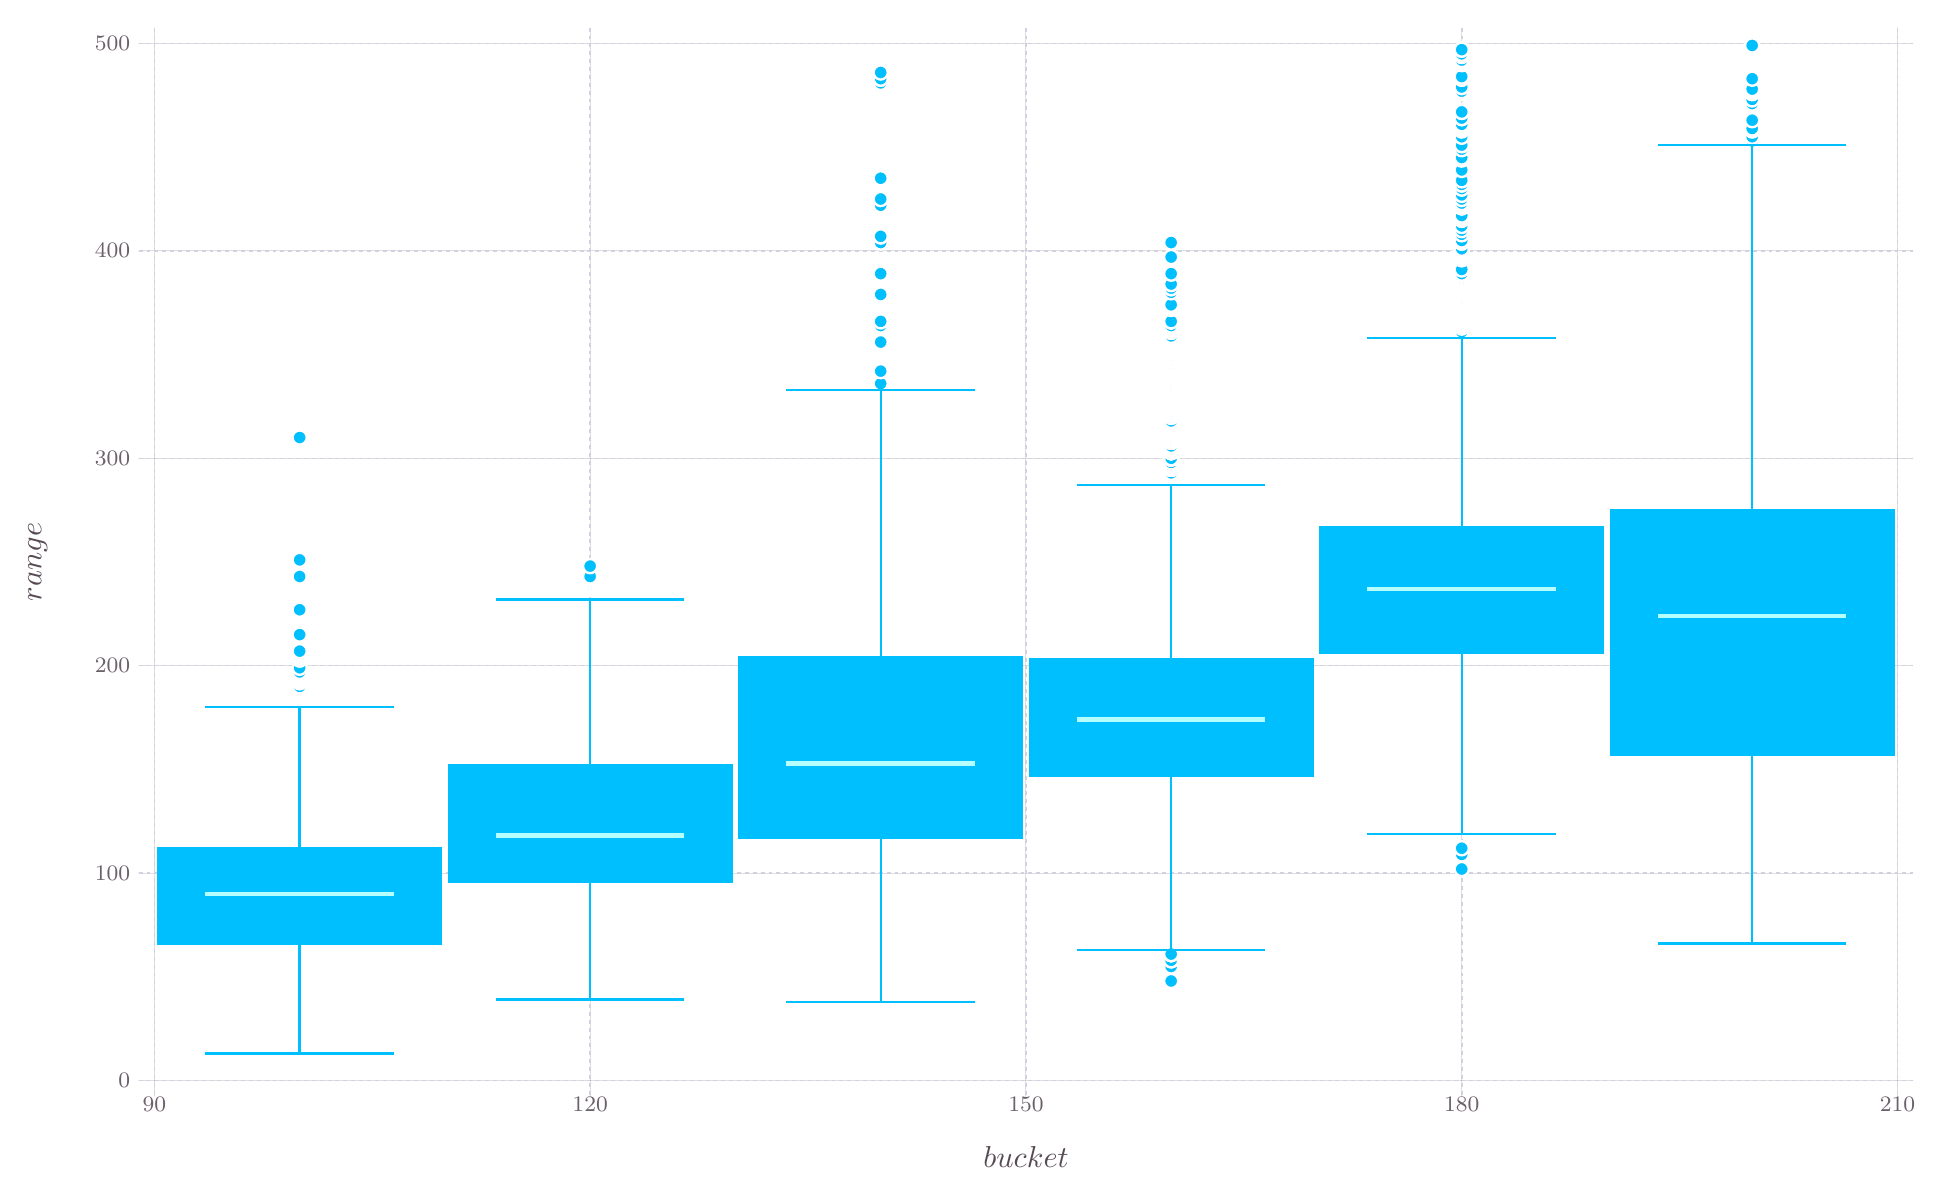
\begin{tikzpicture}[x=1mm,y=-1mm]
\definecolor{mycolor00BFFF}{rgb}{0,0.75,1}
\definecolor{mycolorD0D0E0}{rgb}{0.82,0.82,0.88}
\definecolor{mycolor000000}{rgb}{0,0,0}
\definecolor{mycolor564A55}{rgb}{0.34,0.29,0.33}
\definecolor{mycolor000000}{rgb}{0,0,0}
\definecolor{mycolorFFFFFF}{rgb}{1,1,1}
\definecolor{mycolorB5FFFF}{rgb}{0.71,1,1}
\definecolor{mycolor6C606B}{rgb}{0.42,0.38,0.42}
\begin{scope}
\begin{scope}
\draw (132.32,148.39) node [text=mycolor564A55,draw=mycolor000000,draw opacity=0,rotate around={-0: (0,1.81)},inner sep=0.0]{\fontsize{3.88mm}{4.66mm}\selectfont $\text{bucket}$};
\end{scope}
\begin{scope}
\draw (21.63,141.72) node [text=mycolor6C606B,rotate around={-0: (110.68,1.34)},inner sep=0.0]{\fontsize{2.82mm}{3.39mm}\selectfont $\text{90}$};
\draw (76.97,141.72) node [text=mycolor6C606B,rotate around={-0: (55.34,1.34)},inner sep=0.0]{\fontsize{2.82mm}{3.39mm}\selectfont $\text{120}$};
\draw (132.32,141.72) node [text=mycolor6C606B,rotate around={-0: (0,1.34)},inner sep=0.0]{\fontsize{2.82mm}{3.39mm}\selectfont $\text{150}$};
\draw (187.66,141.72) node [text=mycolor6C606B,rotate around={-0: (-55.34,1.34)},inner sep=0.0]{\fontsize{2.82mm}{3.39mm}\selectfont $\text{180}$};
\draw (243,141.72) node [text=mycolor6C606B,rotate around={-0: (-110.68,1.34)},inner sep=0.0]{\fontsize{2.82mm}{3.39mm}\selectfont $\text{210}$};
\end{scope}
\begin{scope}
\clip  (19.63,5) -- (245,5) -- (245,140.72) -- (19.63,140.72);
\begin{scope}
\clip  (19.63,5) -- (245,5) -- (245,140.72) -- (19.63,140.72);
\path [fill=mycolor000000,fill opacity=0,draw=mycolor000000,draw opacity=0] (19.63,5) rectangle +(225.37,135.72);
\end{scope}
\begin{scope}
[dash pattern=on 0.5mm off 0.5mm,line width=0.2mm]
\path [fill=mycolor000000,draw=mycolorD0D0E0]  (19.63,138.72) -- (245,138.72);
\path [fill=mycolor000000,draw=mycolorD0D0E0]  (19.63,112.37) -- (245,112.37);
\path [fill=mycolor000000,draw=mycolorD0D0E0]  (19.63,86.03) -- (245,86.03);
\path [fill=mycolor000000,draw=mycolorD0D0E0]  (19.63,59.69) -- (245,59.69);
\path [fill=mycolor000000,draw=mycolorD0D0E0]  (19.63,33.34) -- (245,33.34);
\path [fill=mycolor000000,draw=mycolorD0D0E0]  (19.63,7) -- (245,7);
\end{scope}
\begin{scope}
[dash pattern=on 0.5mm off 0.5mm,line width=0.2mm]
\path [fill=mycolor000000,draw=mycolorD0D0E0]  (21.63,5) -- (21.63,140.72);
\path [fill=mycolor000000,draw=mycolorD0D0E0]  (76.97,5) -- (76.97,140.72);
\path [fill=mycolor000000,draw=mycolorD0D0E0]  (132.32,5) -- (132.32,140.72);
\path [fill=mycolor000000,draw=mycolorD0D0E0]  (187.66,5) -- (187.66,140.72);
\path [fill=mycolor000000,draw=mycolorD0D0E0]  (243,5) -- (243,140.72);
\end{scope}
\begin{scope}
\begin{scope}
[line width=0.3mm]
\path [fill=mycolor00BFFF,draw=mycolorFFFFFF] (40.08,90.77) circle [radius=0.9];
\path [fill=mycolor00BFFF,draw=mycolorFFFFFF] (40.08,90.77) circle [radius=0.9];
\path [fill=mycolor00BFFF,draw=mycolorFFFFFF] (40.08,90.77) circle [radius=0.9];
\path [fill=mycolor00BFFF,draw=mycolorFFFFFF] (40.08,90.77) circle [radius=0.9];
\path [fill=mycolor00BFFF,draw=mycolorFFFFFF] (40.08,90.77) circle [radius=0.9];
\path [fill=mycolor00BFFF,draw=mycolorFFFFFF] (40.08,90.51) circle [radius=0.9];
\path [fill=mycolor00BFFF,draw=mycolorFFFFFF] (40.08,90.51) circle [radius=0.9];
\path [fill=mycolor00BFFF,draw=mycolorFFFFFF] (40.08,90.51) circle [radius=0.9];
\path [fill=mycolor00BFFF,draw=mycolorFFFFFF] (40.08,90.51) circle [radius=0.9];
\path [fill=mycolor00BFFF,draw=mycolorFFFFFF] (40.08,90.51) circle [radius=0.9];
\path [fill=mycolor00BFFF,draw=mycolorFFFFFF] (40.08,90.24) circle [radius=0.9];
\path [fill=mycolor00BFFF,draw=mycolorFFFFFF] (40.08,89.98) circle [radius=0.9];
\path [fill=mycolor00BFFF,draw=mycolorFFFFFF] (40.08,89.98) circle [radius=0.9];
\path [fill=mycolor00BFFF,draw=mycolorFFFFFF] (40.08,89.72) circle [radius=0.9];
\path [fill=mycolor00BFFF,draw=mycolorFFFFFF] (40.08,89.72) circle [radius=0.9];
\path [fill=mycolor00BFFF,draw=mycolorFFFFFF] (40.08,89.72) circle [radius=0.9];
\path [fill=mycolor00BFFF,draw=mycolorFFFFFF] (40.08,89.72) circle [radius=0.9];
\path [fill=mycolor00BFFF,draw=mycolorFFFFFF] (40.08,89.72) circle [radius=0.9];
\path [fill=mycolor00BFFF,draw=mycolorFFFFFF] (40.08,89.72) circle [radius=0.9];
\path [fill=mycolor00BFFF,draw=mycolorFFFFFF] (40.08,89.45) circle [radius=0.9];
\path [fill=mycolor00BFFF,draw=mycolorFFFFFF] (40.08,89.45) circle [radius=0.9];
\path [fill=mycolor00BFFF,draw=mycolorFFFFFF] (40.08,89.19) circle [radius=0.9];
\path [fill=mycolor00BFFF,draw=mycolorFFFFFF] (40.08,89.19) circle [radius=0.9];
\path [fill=mycolor00BFFF,draw=mycolorFFFFFF] (40.08,89.19) circle [radius=0.9];
\path [fill=mycolor00BFFF,draw=mycolorFFFFFF] (40.08,89.19) circle [radius=0.9];
\path [fill=mycolor00BFFF,draw=mycolorFFFFFF] (40.08,88.93) circle [radius=0.9];
\path [fill=mycolor00BFFF,draw=mycolorFFFFFF] (40.08,88.93) circle [radius=0.9];
\path [fill=mycolor00BFFF,draw=mycolorFFFFFF] (40.08,88.93) circle [radius=0.9];
\path [fill=mycolor00BFFF,draw=mycolorFFFFFF] (40.08,88.66) circle [radius=0.9];
\path [fill=mycolor00BFFF,draw=mycolorFFFFFF] (40.08,88.66) circle [radius=0.9];
\path [fill=mycolor00BFFF,draw=mycolorFFFFFF] (40.08,88.66) circle [radius=0.9];
\path [fill=mycolor00BFFF,draw=mycolorFFFFFF] (40.08,88.14) circle [radius=0.9];
\path [fill=mycolor00BFFF,draw=mycolorFFFFFF] (40.08,87.87) circle [radius=0.9];
\path [fill=mycolor00BFFF,draw=mycolorFFFFFF] (40.08,87.87) circle [radius=0.9];
\path [fill=mycolor00BFFF,draw=mycolorFFFFFF] (40.08,87.87) circle [radius=0.9];
\path [fill=mycolor00BFFF,draw=mycolorFFFFFF] (40.08,87.87) circle [radius=0.9];
\path [fill=mycolor00BFFF,draw=mycolorFFFFFF] (40.08,87.61) circle [radius=0.9];
\path [fill=mycolor00BFFF,draw=mycolorFFFFFF] (40.08,87.35) circle [radius=0.9];
\path [fill=mycolor00BFFF,draw=mycolorFFFFFF] (40.08,87.08) circle [radius=0.9];
\path [fill=mycolor00BFFF,draw=mycolorFFFFFF] (40.08,87.08) circle [radius=0.9];
\path [fill=mycolor00BFFF,draw=mycolorFFFFFF] (40.08,86.82) circle [radius=0.9];
\path [fill=mycolor00BFFF,draw=mycolorFFFFFF] (40.08,86.29) circle [radius=0.9];
\path [fill=mycolor00BFFF,draw=mycolorFFFFFF] (40.08,85.24) circle [radius=0.9];
\path [fill=mycolor00BFFF,draw=mycolorFFFFFF] (40.08,85.24) circle [radius=0.9];
\path [fill=mycolor00BFFF,draw=mycolorFFFFFF] (40.08,84.98) circle [radius=0.9];
\path [fill=mycolor00BFFF,draw=mycolorFFFFFF] (40.08,84.71) circle [radius=0.9];
\path [fill=mycolor00BFFF,draw=mycolorFFFFFF] (40.08,84.45) circle [radius=0.9];
\path [fill=mycolor00BFFF,draw=mycolorFFFFFF] (40.08,84.18) circle [radius=0.9];
\path [fill=mycolor00BFFF,draw=mycolorFFFFFF] (40.08,82.08) circle [radius=0.9];
\path [fill=mycolor00BFFF,draw=mycolorFFFFFF] (40.08,78.92) circle [radius=0.9];
\path [fill=mycolor00BFFF,draw=mycolorFFFFFF] (40.08,74.7) circle [radius=0.9];
\path [fill=mycolor00BFFF,draw=mycolorFFFFFF] (40.08,72.59) circle [radius=0.9];
\path [fill=mycolor00BFFF,draw=mycolorFFFFFF] (40.08,57.05) circle [radius=0.9];
\path [fill=mycolor00BFFF,draw=mycolorFFFFFF] (76.97,76.28) circle [radius=0.9];
\path [fill=mycolor00BFFF,draw=mycolorFFFFFF] (76.97,76.02) circle [radius=0.9];
\path [fill=mycolor00BFFF,draw=mycolorFFFFFF] (76.97,76.02) circle [radius=0.9];
\path [fill=mycolor00BFFF,draw=mycolorFFFFFF] (76.97,75.76) circle [radius=0.9];
\path [fill=mycolor00BFFF,draw=mycolorFFFFFF] (76.97,75.76) circle [radius=0.9];
\path [fill=mycolor00BFFF,draw=mycolorFFFFFF] (76.97,75.49) circle [radius=0.9];
\path [fill=mycolor00BFFF,draw=mycolorFFFFFF] (76.97,75.23) circle [radius=0.9];
\path [fill=mycolor00BFFF,draw=mycolorFFFFFF] (76.97,74.96) circle [radius=0.9];
\path [fill=mycolor00BFFF,draw=mycolorFFFFFF] (76.97,74.7) circle [radius=0.9];
\path [fill=mycolor00BFFF,draw=mycolorFFFFFF] (76.97,74.7) circle [radius=0.9];
\path [fill=mycolor00BFFF,draw=mycolorFFFFFF] (76.97,74.7) circle [radius=0.9];
\path [fill=mycolor00BFFF,draw=mycolorFFFFFF] (76.97,74.7) circle [radius=0.9];
\path [fill=mycolor00BFFF,draw=mycolorFFFFFF] (76.97,73.38) circle [radius=0.9];
\path [fill=mycolor00BFFF,draw=mycolorFFFFFF] (113.87,50.2) circle [radius=0.9];
\path [fill=mycolor00BFFF,draw=mycolorFFFFFF] (113.87,48.62) circle [radius=0.9];
\path [fill=mycolor00BFFF,draw=mycolorFFFFFF] (113.87,44.93) circle [radius=0.9];
\path [fill=mycolor00BFFF,draw=mycolorFFFFFF] (113.87,42.83) circle [radius=0.9];
\path [fill=mycolor00BFFF,draw=mycolorFFFFFF] (113.87,42.3) circle [radius=0.9];
\path [fill=mycolor00BFFF,draw=mycolorFFFFFF] (113.87,38.88) circle [radius=0.9];
\path [fill=mycolor00BFFF,draw=mycolorFFFFFF] (113.87,36.24) circle [radius=0.9];
\path [fill=mycolor00BFFF,draw=mycolorFFFFFF] (113.87,32.29) circle [radius=0.9];
\path [fill=mycolor00BFFF,draw=mycolorFFFFFF] (113.87,31.5) circle [radius=0.9];
\path [fill=mycolor00BFFF,draw=mycolorFFFFFF] (113.87,31.5) circle [radius=0.9];
\path [fill=mycolor00BFFF,draw=mycolorFFFFFF] (113.87,27.55) circle [radius=0.9];
\path [fill=mycolor00BFFF,draw=mycolorFFFFFF] (113.87,26.76) circle [radius=0.9];
\path [fill=mycolor00BFFF,draw=mycolorFFFFFF] (113.87,24.12) circle [radius=0.9];
\path [fill=mycolor00BFFF,draw=mycolorFFFFFF] (113.87,12.01) circle [radius=0.9];
\path [fill=mycolor00BFFF,draw=mycolorFFFFFF] (113.87,11.48) circle [radius=0.9];
\path [fill=mycolor00BFFF,draw=mycolorFFFFFF] (113.87,11.48) circle [radius=0.9];
\path [fill=mycolor00BFFF,draw=mycolorFFFFFF] (113.87,10.69) circle [radius=0.9];
\path [fill=mycolor00BFFF,draw=mycolorFFFFFF] (150.76,126.07) circle [radius=0.9];
\path [fill=mycolor00BFFF,draw=mycolorFFFFFF] (150.76,124.23) circle [radius=0.9];
\path [fill=mycolor00BFFF,draw=mycolorFFFFFF] (150.76,124.23) circle [radius=0.9];
\path [fill=mycolor00BFFF,draw=mycolorFFFFFF] (150.76,123.44) circle [radius=0.9];
\path [fill=mycolor00BFFF,draw=mycolorFFFFFF] (150.76,123.44) circle [radius=0.9];
\path [fill=mycolor00BFFF,draw=mycolorFFFFFF] (150.76,122.65) circle [radius=0.9];
\path [fill=mycolor00BFFF,draw=mycolorFFFFFF] (150.76,122.65) circle [radius=0.9];
\path [fill=mycolor00BFFF,draw=mycolorFFFFFF] (150.76,122.65) circle [radius=0.9];
\path [fill=mycolor00BFFF,draw=mycolorFFFFFF] (150.76,122.65) circle [radius=0.9];
\path [fill=mycolor00BFFF,draw=mycolorFFFFFF] (150.76,122.65) circle [radius=0.9];
\path [fill=mycolor00BFFF,draw=mycolorFFFFFF] (150.76,62.85) circle [radius=0.9];
\path [fill=mycolor00BFFF,draw=mycolorFFFFFF] (150.76,62.85) circle [radius=0.9];
\path [fill=mycolor00BFFF,draw=mycolorFFFFFF] (150.76,62.58) circle [radius=0.9];
\path [fill=mycolor00BFFF,draw=mycolorFFFFFF] (150.76,62.32) circle [radius=0.9];
\path [fill=mycolor00BFFF,draw=mycolorFFFFFF] (150.76,62.32) circle [radius=0.9];
\path [fill=mycolor00BFFF,draw=mycolorFFFFFF] (150.76,62.32) circle [radius=0.9];
\path [fill=mycolor00BFFF,draw=mycolorFFFFFF] (150.76,62.32) circle [radius=0.9];
\path [fill=mycolor00BFFF,draw=mycolorFFFFFF] (150.76,62.32) circle [radius=0.9];
\path [fill=mycolor00BFFF,draw=mycolorFFFFFF] (150.76,62.32) circle [radius=0.9];
\path [fill=mycolor00BFFF,draw=mycolorFFFFFF] (150.76,62.32) circle [radius=0.9];
\path [fill=mycolor00BFFF,draw=mycolorFFFFFF] (150.76,62.32) circle [radius=0.9];
\path [fill=mycolor00BFFF,draw=mycolorFFFFFF] (150.76,62.32) circle [radius=0.9];
\path [fill=mycolor00BFFF,draw=mycolorFFFFFF] (150.76,62.32) circle [radius=0.9];
\path [fill=mycolor00BFFF,draw=mycolorFFFFFF] (150.76,62.32) circle [radius=0.9];
\path [fill=mycolor00BFFF,draw=mycolorFFFFFF] (150.76,62.32) circle [radius=0.9];
\path [fill=mycolor00BFFF,draw=mycolorFFFFFF] (150.76,62.32) circle [radius=0.9];
\path [fill=mycolor00BFFF,draw=mycolorFFFFFF] (150.76,62.32) circle [radius=0.9];
\path [fill=mycolor00BFFF,draw=mycolorFFFFFF] (150.76,62.32) circle [radius=0.9];
\path [fill=mycolor00BFFF,draw=mycolorFFFFFF] (150.76,62.32) circle [radius=0.9];
\path [fill=mycolor00BFFF,draw=mycolorFFFFFF] (150.76,62.32) circle [radius=0.9];
\path [fill=mycolor00BFFF,draw=mycolorFFFFFF] (150.76,62.06) circle [radius=0.9];
\path [fill=mycolor00BFFF,draw=mycolorFFFFFF] (150.76,62.06) circle [radius=0.9];
\path [fill=mycolor00BFFF,draw=mycolorFFFFFF] (150.76,61.79) circle [radius=0.9];
\path [fill=mycolor00BFFF,draw=mycolorFFFFFF] (150.76,61.79) circle [radius=0.9];
\path [fill=mycolor00BFFF,draw=mycolorFFFFFF] (150.76,61.79) circle [radius=0.9];
\path [fill=mycolor00BFFF,draw=mycolorFFFFFF] (150.76,61.79) circle [radius=0.9];
\path [fill=mycolor00BFFF,draw=mycolorFFFFFF] (150.76,61.79) circle [radius=0.9];
\path [fill=mycolor00BFFF,draw=mycolorFFFFFF] (150.76,61.79) circle [radius=0.9];
\path [fill=mycolor00BFFF,draw=mycolorFFFFFF] (150.76,61.53) circle [radius=0.9];
\path [fill=mycolor00BFFF,draw=mycolorFFFFFF] (150.76,61) circle [radius=0.9];
\path [fill=mycolor00BFFF,draw=mycolorFFFFFF] (150.76,61) circle [radius=0.9];
\path [fill=mycolor00BFFF,draw=mycolorFFFFFF] (150.76,61) circle [radius=0.9];
\path [fill=mycolor00BFFF,draw=mycolorFFFFFF] (150.76,61) circle [radius=0.9];
\path [fill=mycolor00BFFF,draw=mycolorFFFFFF] (150.76,61) circle [radius=0.9];
\path [fill=mycolor00BFFF,draw=mycolorFFFFFF] (150.76,61) circle [radius=0.9];
\path [fill=mycolor00BFFF,draw=mycolorFFFFFF] (150.76,61) circle [radius=0.9];
\path [fill=mycolor00BFFF,draw=mycolorFFFFFF] (150.76,61) circle [radius=0.9];
\path [fill=mycolor00BFFF,draw=mycolorFFFFFF] (150.76,61) circle [radius=0.9];
\path [fill=mycolor00BFFF,draw=mycolorFFFFFF] (150.76,61) circle [radius=0.9];
\path [fill=mycolor00BFFF,draw=mycolorFFFFFF] (150.76,61) circle [radius=0.9];
\path [fill=mycolor00BFFF,draw=mycolorFFFFFF] (150.76,61) circle [radius=0.9];
\path [fill=mycolor00BFFF,draw=mycolorFFFFFF] (150.76,61) circle [radius=0.9];
\path [fill=mycolor00BFFF,draw=mycolorFFFFFF] (150.76,61) circle [radius=0.9];
\path [fill=mycolor00BFFF,draw=mycolorFFFFFF] (150.76,61) circle [radius=0.9];
\path [fill=mycolor00BFFF,draw=mycolorFFFFFF] (150.76,61) circle [radius=0.9];
\path [fill=mycolor00BFFF,draw=mycolorFFFFFF] (150.76,61) circle [radius=0.9];
\path [fill=mycolor00BFFF,draw=mycolorFFFFFF] (150.76,60.74) circle [radius=0.9];
\path [fill=mycolor00BFFF,draw=mycolorFFFFFF] (150.76,60.74) circle [radius=0.9];
\path [fill=mycolor00BFFF,draw=mycolorFFFFFF] (150.76,60.74) circle [radius=0.9];
\path [fill=mycolor00BFFF,draw=mycolorFFFFFF] (150.76,60.74) circle [radius=0.9];
\path [fill=mycolor00BFFF,draw=mycolorFFFFFF] (150.76,60.74) circle [radius=0.9];
\path [fill=mycolor00BFFF,draw=mycolorFFFFFF] (150.76,60.48) circle [radius=0.9];
\path [fill=mycolor00BFFF,draw=mycolorFFFFFF] (150.76,60.48) circle [radius=0.9];
\path [fill=mycolor00BFFF,draw=mycolorFFFFFF] (150.76,60.48) circle [radius=0.9];
\path [fill=mycolor00BFFF,draw=mycolorFFFFFF] (150.76,60.48) circle [radius=0.9];
\path [fill=mycolor00BFFF,draw=mycolorFFFFFF] (150.76,60.48) circle [radius=0.9];
\path [fill=mycolor00BFFF,draw=mycolorFFFFFF] (150.76,60.48) circle [radius=0.9];
\path [fill=mycolor00BFFF,draw=mycolorFFFFFF] (150.76,60.48) circle [radius=0.9];
\path [fill=mycolor00BFFF,draw=mycolorFFFFFF] (150.76,60.21) circle [radius=0.9];
\path [fill=mycolor00BFFF,draw=mycolorFFFFFF] (150.76,60.21) circle [radius=0.9];
\path [fill=mycolor00BFFF,draw=mycolorFFFFFF] (150.76,59.69) circle [radius=0.9];
\path [fill=mycolor00BFFF,draw=mycolorFFFFFF] (150.76,59.69) circle [radius=0.9];
\path [fill=mycolor00BFFF,draw=mycolorFFFFFF] (150.76,59.69) circle [radius=0.9];
\path [fill=mycolor00BFFF,draw=mycolorFFFFFF] (150.76,59.69) circle [radius=0.9];
\path [fill=mycolor00BFFF,draw=mycolorFFFFFF] (150.76,59.69) circle [radius=0.9];
\path [fill=mycolor00BFFF,draw=mycolorFFFFFF] (150.76,59.69) circle [radius=0.9];
\path [fill=mycolor00BFFF,draw=mycolorFFFFFF] (150.76,59.69) circle [radius=0.9];
\path [fill=mycolor00BFFF,draw=mycolorFFFFFF] (150.76,59.69) circle [radius=0.9];
\path [fill=mycolor00BFFF,draw=mycolorFFFFFF] (150.76,59.69) circle [radius=0.9];
\path [fill=mycolor00BFFF,draw=mycolorFFFFFF] (150.76,59.69) circle [radius=0.9];
\path [fill=mycolor00BFFF,draw=mycolorFFFFFF] (150.76,59.69) circle [radius=0.9];
\path [fill=mycolor00BFFF,draw=mycolorFFFFFF] (150.76,58.9) circle [radius=0.9];
\path [fill=mycolor00BFFF,draw=mycolorFFFFFF] (150.76,58.9) circle [radius=0.9];
\path [fill=mycolor00BFFF,draw=mycolorFFFFFF] (150.76,58.9) circle [radius=0.9];
\path [fill=mycolor00BFFF,draw=mycolorFFFFFF] (150.76,58.9) circle [radius=0.9];
\path [fill=mycolor00BFFF,draw=mycolorFFFFFF] (150.76,58.9) circle [radius=0.9];
\path [fill=mycolor00BFFF,draw=mycolorFFFFFF] (150.76,58.9) circle [radius=0.9];
\path [fill=mycolor00BFFF,draw=mycolorFFFFFF] (150.76,58.9) circle [radius=0.9];
\path [fill=mycolor00BFFF,draw=mycolorFFFFFF] (150.76,58.63) circle [radius=0.9];
\path [fill=mycolor00BFFF,draw=mycolorFFFFFF] (150.76,58.63) circle [radius=0.9];
\path [fill=mycolor00BFFF,draw=mycolorFFFFFF] (150.76,58.37) circle [radius=0.9];
\path [fill=mycolor00BFFF,draw=mycolorFFFFFF] (150.76,58.37) circle [radius=0.9];
\path [fill=mycolor00BFFF,draw=mycolorFFFFFF] (150.76,58.37) circle [radius=0.9];
\path [fill=mycolor00BFFF,draw=mycolorFFFFFF] (150.76,58.37) circle [radius=0.9];
\path [fill=mycolor00BFFF,draw=mycolorFFFFFF] (150.76,58.11) circle [radius=0.9];
\path [fill=mycolor00BFFF,draw=mycolorFFFFFF] (150.76,58.11) circle [radius=0.9];
\path [fill=mycolor00BFFF,draw=mycolorFFFFFF] (150.76,58.11) circle [radius=0.9];
\path [fill=mycolor00BFFF,draw=mycolorFFFFFF] (150.76,57.58) circle [radius=0.9];
\path [fill=mycolor00BFFF,draw=mycolorFFFFFF] (150.76,57.58) circle [radius=0.9];
\path [fill=mycolor00BFFF,draw=mycolorFFFFFF] (150.76,57.58) circle [radius=0.9];
\path [fill=mycolor00BFFF,draw=mycolorFFFFFF] (150.76,57.58) circle [radius=0.9];
\path [fill=mycolor00BFFF,draw=mycolorFFFFFF] (150.76,57.58) circle [radius=0.9];
\path [fill=mycolor00BFFF,draw=mycolorFFFFFF] (150.76,57.58) circle [radius=0.9];
\path [fill=mycolor00BFFF,draw=mycolorFFFFFF] (150.76,57.58) circle [radius=0.9];
\path [fill=mycolor00BFFF,draw=mycolorFFFFFF] (150.76,57.32) circle [radius=0.9];
\path [fill=mycolor00BFFF,draw=mycolorFFFFFF] (150.76,57.32) circle [radius=0.9];
\path [fill=mycolor00BFFF,draw=mycolorFFFFFF] (150.76,57.32) circle [radius=0.9];
\path [fill=mycolor00BFFF,draw=mycolorFFFFFF] (150.76,57.05) circle [radius=0.9];
\path [fill=mycolor00BFFF,draw=mycolorFFFFFF] (150.76,57.05) circle [radius=0.9];
\path [fill=mycolor00BFFF,draw=mycolorFFFFFF] (150.76,57.05) circle [radius=0.9];
\path [fill=mycolor00BFFF,draw=mycolorFFFFFF] (150.76,57.05) circle [radius=0.9];
\path [fill=mycolor00BFFF,draw=mycolorFFFFFF] (150.76,57.05) circle [radius=0.9];
\path [fill=mycolor00BFFF,draw=mycolorFFFFFF] (150.76,57.05) circle [radius=0.9];
\path [fill=mycolor00BFFF,draw=mycolorFFFFFF] (150.76,57.05) circle [radius=0.9];
\path [fill=mycolor00BFFF,draw=mycolorFFFFFF] (150.76,57.05) circle [radius=0.9];
\path [fill=mycolor00BFFF,draw=mycolorFFFFFF] (150.76,57.05) circle [radius=0.9];
\path [fill=mycolor00BFFF,draw=mycolorFFFFFF] (150.76,57.05) circle [radius=0.9];
\path [fill=mycolor00BFFF,draw=mycolorFFFFFF] (150.76,57.05) circle [radius=0.9];
\path [fill=mycolor00BFFF,draw=mycolorFFFFFF] (150.76,57.05) circle [radius=0.9];
\path [fill=mycolor00BFFF,draw=mycolorFFFFFF] (150.76,57.05) circle [radius=0.9];
\path [fill=mycolor00BFFF,draw=mycolorFFFFFF] (150.76,56.79) circle [radius=0.9];
\path [fill=mycolor00BFFF,draw=mycolorFFFFFF] (150.76,56.52) circle [radius=0.9];
\path [fill=mycolor00BFFF,draw=mycolorFFFFFF] (150.76,56.52) circle [radius=0.9];
\path [fill=mycolor00BFFF,draw=mycolorFFFFFF] (150.76,56.26) circle [radius=0.9];
\path [fill=mycolor00BFFF,draw=mycolorFFFFFF] (150.76,56.26) circle [radius=0.9];
\path [fill=mycolor00BFFF,draw=mycolorFFFFFF] (150.76,56.26) circle [radius=0.9];
\path [fill=mycolor00BFFF,draw=mycolorFFFFFF] (150.76,56) circle [radius=0.9];
\path [fill=mycolor00BFFF,draw=mycolorFFFFFF] (150.76,55.73) circle [radius=0.9];
\path [fill=mycolor00BFFF,draw=mycolorFFFFFF] (150.76,55.73) circle [radius=0.9];
\path [fill=mycolor00BFFF,draw=mycolorFFFFFF] (150.76,55.73) circle [radius=0.9];
\path [fill=mycolor00BFFF,draw=mycolorFFFFFF] (150.76,55.73) circle [radius=0.9];
\path [fill=mycolor00BFFF,draw=mycolorFFFFFF] (150.76,55.73) circle [radius=0.9];
\path [fill=mycolor00BFFF,draw=mycolorFFFFFF] (150.76,55.73) circle [radius=0.9];
\path [fill=mycolor00BFFF,draw=mycolorFFFFFF] (150.76,55.73) circle [radius=0.9];
\path [fill=mycolor00BFFF,draw=mycolorFFFFFF] (150.76,55.73) circle [radius=0.9];
\path [fill=mycolor00BFFF,draw=mycolorFFFFFF] (150.76,55.73) circle [radius=0.9];
\path [fill=mycolor00BFFF,draw=mycolorFFFFFF] (150.76,55.47) circle [radius=0.9];
\path [fill=mycolor00BFFF,draw=mycolorFFFFFF] (150.76,55.21) circle [radius=0.9];
\path [fill=mycolor00BFFF,draw=mycolorFFFFFF] (150.76,55.21) circle [radius=0.9];
\path [fill=mycolor00BFFF,draw=mycolorFFFFFF] (150.76,55.21) circle [radius=0.9];
\path [fill=mycolor00BFFF,draw=mycolorFFFFFF] (150.76,55.21) circle [radius=0.9];
\path [fill=mycolor00BFFF,draw=mycolorFFFFFF] (150.76,55.21) circle [radius=0.9];
\path [fill=mycolor00BFFF,draw=mycolorFFFFFF] (150.76,55.21) circle [radius=0.9];
\path [fill=mycolor00BFFF,draw=mycolorFFFFFF] (150.76,55.21) circle [radius=0.9];
\path [fill=mycolor00BFFF,draw=mycolorFFFFFF] (150.76,55.21) circle [radius=0.9];
\path [fill=mycolor00BFFF,draw=mycolorFFFFFF] (150.76,54.94) circle [radius=0.9];
\path [fill=mycolor00BFFF,draw=mycolorFFFFFF] (150.76,54.94) circle [radius=0.9];
\path [fill=mycolor00BFFF,draw=mycolorFFFFFF] (150.76,54.94) circle [radius=0.9];
\path [fill=mycolor00BFFF,draw=mycolorFFFFFF] (150.76,54.94) circle [radius=0.9];
\path [fill=mycolor00BFFF,draw=mycolorFFFFFF] (150.76,54.42) circle [radius=0.9];
\path [fill=mycolor00BFFF,draw=mycolorFFFFFF] (150.76,54.42) circle [radius=0.9];
\path [fill=mycolor00BFFF,draw=mycolorFFFFFF] (150.76,54.15) circle [radius=0.9];
\path [fill=mycolor00BFFF,draw=mycolorFFFFFF] (150.76,53.89) circle [radius=0.9];
\path [fill=mycolor00BFFF,draw=mycolorFFFFFF] (150.76,53.89) circle [radius=0.9];
\path [fill=mycolor00BFFF,draw=mycolorFFFFFF] (150.76,53.63) circle [radius=0.9];
\path [fill=mycolor00BFFF,draw=mycolorFFFFFF] (150.76,53.36) circle [radius=0.9];
\path [fill=mycolor00BFFF,draw=mycolorFFFFFF] (150.76,53.36) circle [radius=0.9];
\path [fill=mycolor00BFFF,draw=mycolorFFFFFF] (150.76,53.1) circle [radius=0.9];
\path [fill=mycolor00BFFF,draw=mycolorFFFFFF] (150.76,53.1) circle [radius=0.9];
\path [fill=mycolor00BFFF,draw=mycolorFFFFFF] (150.76,52.84) circle [radius=0.9];
\path [fill=mycolor00BFFF,draw=mycolorFFFFFF] (150.76,52.57) circle [radius=0.9];
\path [fill=mycolor00BFFF,draw=mycolorFFFFFF] (150.76,52.57) circle [radius=0.9];
\path [fill=mycolor00BFFF,draw=mycolorFFFFFF] (150.76,52.57) circle [radius=0.9];
\path [fill=mycolor00BFFF,draw=mycolorFFFFFF] (150.76,52.57) circle [radius=0.9];
\path [fill=mycolor00BFFF,draw=mycolorFFFFFF] (150.76,52.31) circle [radius=0.9];
\path [fill=mycolor00BFFF,draw=mycolorFFFFFF] (150.76,52.31) circle [radius=0.9];
\path [fill=mycolor00BFFF,draw=mycolorFFFFFF] (150.76,52.31) circle [radius=0.9];
\path [fill=mycolor00BFFF,draw=mycolorFFFFFF] (150.76,52.05) circle [radius=0.9];
\path [fill=mycolor00BFFF,draw=mycolorFFFFFF] (150.76,52.05) circle [radius=0.9];
\path [fill=mycolor00BFFF,draw=mycolorFFFFFF] (150.76,52.05) circle [radius=0.9];
\path [fill=mycolor00BFFF,draw=mycolorFFFFFF] (150.76,52.05) circle [radius=0.9];
\path [fill=mycolor00BFFF,draw=mycolorFFFFFF] (150.76,52.05) circle [radius=0.9];
\path [fill=mycolor00BFFF,draw=mycolorFFFFFF] (150.76,51.78) circle [radius=0.9];
\path [fill=mycolor00BFFF,draw=mycolorFFFFFF] (150.76,51.52) circle [radius=0.9];
\path [fill=mycolor00BFFF,draw=mycolorFFFFFF] (150.76,51.52) circle [radius=0.9];
\path [fill=mycolor00BFFF,draw=mycolorFFFFFF] (150.76,51.52) circle [radius=0.9];
\path [fill=mycolor00BFFF,draw=mycolorFFFFFF] (150.76,51.26) circle [radius=0.9];
\path [fill=mycolor00BFFF,draw=mycolorFFFFFF] (150.76,51.26) circle [radius=0.9];
\path [fill=mycolor00BFFF,draw=mycolorFFFFFF] (150.76,51.26) circle [radius=0.9];
\path [fill=mycolor00BFFF,draw=mycolorFFFFFF] (150.76,50.99) circle [radius=0.9];
\path [fill=mycolor00BFFF,draw=mycolorFFFFFF] (150.76,50.99) circle [radius=0.9];
\path [fill=mycolor00BFFF,draw=mycolorFFFFFF] (150.76,50.99) circle [radius=0.9];
\path [fill=mycolor00BFFF,draw=mycolorFFFFFF] (150.76,50.99) circle [radius=0.9];
\path [fill=mycolor00BFFF,draw=mycolorFFFFFF] (150.76,50.73) circle [radius=0.9];
\path [fill=mycolor00BFFF,draw=mycolorFFFFFF] (150.76,50.73) circle [radius=0.9];
\path [fill=mycolor00BFFF,draw=mycolorFFFFFF] (150.76,50.73) circle [radius=0.9];
\path [fill=mycolor00BFFF,draw=mycolorFFFFFF] (150.76,50.47) circle [radius=0.9];
\path [fill=mycolor00BFFF,draw=mycolorFFFFFF] (150.76,50.47) circle [radius=0.9];
\path [fill=mycolor00BFFF,draw=mycolorFFFFFF] (150.76,50.47) circle [radius=0.9];
\path [fill=mycolor00BFFF,draw=mycolorFFFFFF] (150.76,50.47) circle [radius=0.9];
\path [fill=mycolor00BFFF,draw=mycolorFFFFFF] (150.76,50.47) circle [radius=0.9];
\path [fill=mycolor00BFFF,draw=mycolorFFFFFF] (150.76,50.47) circle [radius=0.9];
\path [fill=mycolor00BFFF,draw=mycolorFFFFFF] (150.76,50.47) circle [radius=0.9];
\path [fill=mycolor00BFFF,draw=mycolorFFFFFF] (150.76,50.47) circle [radius=0.9];
\path [fill=mycolor00BFFF,draw=mycolorFFFFFF] (150.76,50.47) circle [radius=0.9];
\path [fill=mycolor00BFFF,draw=mycolorFFFFFF] (150.76,50.2) circle [radius=0.9];
\path [fill=mycolor00BFFF,draw=mycolorFFFFFF] (150.76,50.2) circle [radius=0.9];
\path [fill=mycolor00BFFF,draw=mycolorFFFFFF] (150.76,50.2) circle [radius=0.9];
\path [fill=mycolor00BFFF,draw=mycolorFFFFFF] (150.76,49.94) circle [radius=0.9];
\path [fill=mycolor00BFFF,draw=mycolorFFFFFF] (150.76,49.68) circle [radius=0.9];
\path [fill=mycolor00BFFF,draw=mycolorFFFFFF] (150.76,49.68) circle [radius=0.9];
\path [fill=mycolor00BFFF,draw=mycolorFFFFFF] (150.76,49.68) circle [radius=0.9];
\path [fill=mycolor00BFFF,draw=mycolorFFFFFF] (150.76,49.68) circle [radius=0.9];
\path [fill=mycolor00BFFF,draw=mycolorFFFFFF] (150.76,49.68) circle [radius=0.9];
\path [fill=mycolor00BFFF,draw=mycolorFFFFFF] (150.76,49.68) circle [radius=0.9];
\path [fill=mycolor00BFFF,draw=mycolorFFFFFF] (150.76,49.68) circle [radius=0.9];
\path [fill=mycolor00BFFF,draw=mycolorFFFFFF] (150.76,49.68) circle [radius=0.9];
\path [fill=mycolor00BFFF,draw=mycolorFFFFFF] (150.76,49.68) circle [radius=0.9];
\path [fill=mycolor00BFFF,draw=mycolorFFFFFF] (150.76,49.41) circle [radius=0.9];
\path [fill=mycolor00BFFF,draw=mycolorFFFFFF] (150.76,49.15) circle [radius=0.9];
\path [fill=mycolor00BFFF,draw=mycolorFFFFFF] (150.76,49.15) circle [radius=0.9];
\path [fill=mycolor00BFFF,draw=mycolorFFFFFF] (150.76,49.15) circle [radius=0.9];
\path [fill=mycolor00BFFF,draw=mycolorFFFFFF] (150.76,49.15) circle [radius=0.9];
\path [fill=mycolor00BFFF,draw=mycolorFFFFFF] (150.76,49.15) circle [radius=0.9];
\path [fill=mycolor00BFFF,draw=mycolorFFFFFF] (150.76,49.15) circle [radius=0.9];
\path [fill=mycolor00BFFF,draw=mycolorFFFFFF] (150.76,49.15) circle [radius=0.9];
\path [fill=mycolor00BFFF,draw=mycolorFFFFFF] (150.76,49.15) circle [radius=0.9];
\path [fill=mycolor00BFFF,draw=mycolorFFFFFF] (150.76,48.89) circle [radius=0.9];
\path [fill=mycolor00BFFF,draw=mycolorFFFFFF] (150.76,48.62) circle [radius=0.9];
\path [fill=mycolor00BFFF,draw=mycolorFFFFFF] (150.76,48.62) circle [radius=0.9];
\path [fill=mycolor00BFFF,draw=mycolorFFFFFF] (150.76,48.62) circle [radius=0.9];
\path [fill=mycolor00BFFF,draw=mycolorFFFFFF] (150.76,48.62) circle [radius=0.9];
\path [fill=mycolor00BFFF,draw=mycolorFFFFFF] (150.76,48.62) circle [radius=0.9];
\path [fill=mycolor00BFFF,draw=mycolorFFFFFF] (150.76,48.62) circle [radius=0.9];
\path [fill=mycolor00BFFF,draw=mycolorFFFFFF] (150.76,48.62) circle [radius=0.9];
\path [fill=mycolor00BFFF,draw=mycolorFFFFFF] (150.76,48.36) circle [radius=0.9];
\path [fill=mycolor00BFFF,draw=mycolorFFFFFF] (150.76,48.36) circle [radius=0.9];
\path [fill=mycolor00BFFF,draw=mycolorFFFFFF] (150.76,48.36) circle [radius=0.9];
\path [fill=mycolor00BFFF,draw=mycolorFFFFFF] (150.76,48.36) circle [radius=0.9];
\path [fill=mycolor00BFFF,draw=mycolorFFFFFF] (150.76,48.36) circle [radius=0.9];
\path [fill=mycolor00BFFF,draw=mycolorFFFFFF] (150.76,48.36) circle [radius=0.9];
\path [fill=mycolor00BFFF,draw=mycolorFFFFFF] (150.76,48.36) circle [radius=0.9];
\path [fill=mycolor00BFFF,draw=mycolorFFFFFF] (150.76,48.36) circle [radius=0.9];
\path [fill=mycolor00BFFF,draw=mycolorFFFFFF] (150.76,48.36) circle [radius=0.9];
\path [fill=mycolor00BFFF,draw=mycolorFFFFFF] (150.76,48.36) circle [radius=0.9];
\path [fill=mycolor00BFFF,draw=mycolorFFFFFF] (150.76,48.1) circle [radius=0.9];
\path [fill=mycolor00BFFF,draw=mycolorFFFFFF] (150.76,47.83) circle [radius=0.9];
\path [fill=mycolor00BFFF,draw=mycolorFFFFFF] (150.76,47.83) circle [radius=0.9];
\path [fill=mycolor00BFFF,draw=mycolorFFFFFF] (150.76,47.83) circle [radius=0.9];
\path [fill=mycolor00BFFF,draw=mycolorFFFFFF] (150.76,47.83) circle [radius=0.9];
\path [fill=mycolor00BFFF,draw=mycolorFFFFFF] (150.76,47.83) circle [radius=0.9];
\path [fill=mycolor00BFFF,draw=mycolorFFFFFF] (150.76,47.83) circle [radius=0.9];
\path [fill=mycolor00BFFF,draw=mycolorFFFFFF] (150.76,47.57) circle [radius=0.9];
\path [fill=mycolor00BFFF,draw=mycolorFFFFFF] (150.76,47.57) circle [radius=0.9];
\path [fill=mycolor00BFFF,draw=mycolorFFFFFF] (150.76,47.3) circle [radius=0.9];
\path [fill=mycolor00BFFF,draw=mycolorFFFFFF] (150.76,47.04) circle [radius=0.9];
\path [fill=mycolor00BFFF,draw=mycolorFFFFFF] (150.76,47.04) circle [radius=0.9];
\path [fill=mycolor00BFFF,draw=mycolorFFFFFF] (150.76,47.04) circle [radius=0.9];
\path [fill=mycolor00BFFF,draw=mycolorFFFFFF] (150.76,47.04) circle [radius=0.9];
\path [fill=mycolor00BFFF,draw=mycolorFFFFFF] (150.76,46.78) circle [radius=0.9];
\path [fill=mycolor00BFFF,draw=mycolorFFFFFF] (150.76,46.51) circle [radius=0.9];
\path [fill=mycolor00BFFF,draw=mycolorFFFFFF] (150.76,46.51) circle [radius=0.9];
\path [fill=mycolor00BFFF,draw=mycolorFFFFFF] (150.76,46.51) circle [radius=0.9];
\path [fill=mycolor00BFFF,draw=mycolorFFFFFF] (150.76,46.25) circle [radius=0.9];
\path [fill=mycolor00BFFF,draw=mycolorFFFFFF] (150.76,45.99) circle [radius=0.9];
\path [fill=mycolor00BFFF,draw=mycolorFFFFFF] (150.76,45.99) circle [radius=0.9];
\path [fill=mycolor00BFFF,draw=mycolorFFFFFF] (150.76,45.72) circle [radius=0.9];
\path [fill=mycolor00BFFF,draw=mycolorFFFFFF] (150.76,45.72) circle [radius=0.9];
\path [fill=mycolor00BFFF,draw=mycolorFFFFFF] (150.76,45.72) circle [radius=0.9];
\path [fill=mycolor00BFFF,draw=mycolorFFFFFF] (150.76,45.72) circle [radius=0.9];
\path [fill=mycolor00BFFF,draw=mycolorFFFFFF] (150.76,45.72) circle [radius=0.9];
\path [fill=mycolor00BFFF,draw=mycolorFFFFFF] (150.76,45.46) circle [radius=0.9];
\path [fill=mycolor00BFFF,draw=mycolorFFFFFF] (150.76,45.46) circle [radius=0.9];
\path [fill=mycolor00BFFF,draw=mycolorFFFFFF] (150.76,45.2) circle [radius=0.9];
\path [fill=mycolor00BFFF,draw=mycolorFFFFFF] (150.76,45.2) circle [radius=0.9];
\path [fill=mycolor00BFFF,draw=mycolorFFFFFF] (150.76,44.93) circle [radius=0.9];
\path [fill=mycolor00BFFF,draw=mycolorFFFFFF] (150.76,44.93) circle [radius=0.9];
\path [fill=mycolor00BFFF,draw=mycolorFFFFFF] (150.76,44.93) circle [radius=0.9];
\path [fill=mycolor00BFFF,draw=mycolorFFFFFF] (150.76,44.93) circle [radius=0.9];
\path [fill=mycolor00BFFF,draw=mycolorFFFFFF] (150.76,44.93) circle [radius=0.9];
\path [fill=mycolor00BFFF,draw=mycolorFFFFFF] (150.76,44.93) circle [radius=0.9];
\path [fill=mycolor00BFFF,draw=mycolorFFFFFF] (150.76,44.93) circle [radius=0.9];
\path [fill=mycolor00BFFF,draw=mycolorFFFFFF] (150.76,44.93) circle [radius=0.9];
\path [fill=mycolor00BFFF,draw=mycolorFFFFFF] (150.76,44.93) circle [radius=0.9];
\path [fill=mycolor00BFFF,draw=mycolorFFFFFF] (150.76,44.67) circle [radius=0.9];
\path [fill=mycolor00BFFF,draw=mycolorFFFFFF] (150.76,44.67) circle [radius=0.9];
\path [fill=mycolor00BFFF,draw=mycolorFFFFFF] (150.76,44.67) circle [radius=0.9];
\path [fill=mycolor00BFFF,draw=mycolorFFFFFF] (150.76,44.41) circle [radius=0.9];
\path [fill=mycolor00BFFF,draw=mycolorFFFFFF] (150.76,44.41) circle [radius=0.9];
\path [fill=mycolor00BFFF,draw=mycolorFFFFFF] (150.76,44.14) circle [radius=0.9];
\path [fill=mycolor00BFFF,draw=mycolorFFFFFF] (150.76,43.62) circle [radius=0.9];
\path [fill=mycolor00BFFF,draw=mycolorFFFFFF] (150.76,43.62) circle [radius=0.9];
\path [fill=mycolor00BFFF,draw=mycolorFFFFFF] (150.76,43.62) circle [radius=0.9];
\path [fill=mycolor00BFFF,draw=mycolorFFFFFF] (150.76,43.35) circle [radius=0.9];
\path [fill=mycolor00BFFF,draw=mycolorFFFFFF] (150.76,43.35) circle [radius=0.9];
\path [fill=mycolor00BFFF,draw=mycolorFFFFFF] (150.76,43.09) circle [radius=0.9];
\path [fill=mycolor00BFFF,draw=mycolorFFFFFF] (150.76,43.09) circle [radius=0.9];
\path [fill=mycolor00BFFF,draw=mycolorFFFFFF] (150.76,42.83) circle [radius=0.9];
\path [fill=mycolor00BFFF,draw=mycolorFFFFFF] (150.76,42.3) circle [radius=0.9];
\path [fill=mycolor00BFFF,draw=mycolorFFFFFF] (150.76,42.3) circle [radius=0.9];
\path [fill=mycolor00BFFF,draw=mycolorFFFFFF] (150.76,42.3) circle [radius=0.9];
\path [fill=mycolor00BFFF,draw=mycolorFFFFFF] (150.76,40.72) circle [radius=0.9];
\path [fill=mycolor00BFFF,draw=mycolorFFFFFF] (150.76,40.46) circle [radius=0.9];
\path [fill=mycolor00BFFF,draw=mycolorFFFFFF] (150.76,40.19) circle [radius=0.9];
\path [fill=mycolor00BFFF,draw=mycolorFFFFFF] (150.76,40.19) circle [radius=0.9];
\path [fill=mycolor00BFFF,draw=mycolorFFFFFF] (150.76,38.61) circle [radius=0.9];
\path [fill=mycolor00BFFF,draw=mycolorFFFFFF] (150.76,38.08) circle [radius=0.9];
\path [fill=mycolor00BFFF,draw=mycolorFFFFFF] (150.76,38.08) circle [radius=0.9];
\path [fill=mycolor00BFFF,draw=mycolorFFFFFF] (150.76,37.56) circle [radius=0.9];
\path [fill=mycolor00BFFF,draw=mycolorFFFFFF] (150.76,36.24) circle [radius=0.9];
\path [fill=mycolor00BFFF,draw=mycolorFFFFFF] (150.76,34.13) circle [radius=0.9];
\path [fill=mycolor00BFFF,draw=mycolorFFFFFF] (150.76,32.29) circle [radius=0.9];
\path [fill=mycolor00BFFF,draw=mycolorFFFFFF] (187.66,111.85) circle [radius=0.9];
\path [fill=mycolor00BFFF,draw=mycolorFFFFFF] (187.66,110) circle [radius=0.9];
\path [fill=mycolor00BFFF,draw=mycolorFFFFFF] (187.66,109.21) circle [radius=0.9];
\path [fill=mycolor00BFFF,draw=mycolorFFFFFF] (187.66,44.14) circle [radius=0.9];
\path [fill=mycolor00BFFF,draw=mycolorFFFFFF] (187.66,44.14) circle [radius=0.9];
\path [fill=mycolor00BFFF,draw=mycolorFFFFFF] (187.66,44.14) circle [radius=0.9];
\path [fill=mycolor00BFFF,draw=mycolorFFFFFF] (187.66,43.88) circle [radius=0.9];
\path [fill=mycolor00BFFF,draw=mycolorFFFFFF] (187.66,43.88) circle [radius=0.9];
\path [fill=mycolor00BFFF,draw=mycolorFFFFFF] (187.66,43.62) circle [radius=0.9];
\path [fill=mycolor00BFFF,draw=mycolorFFFFFF] (187.66,43.62) circle [radius=0.9];
\path [fill=mycolor00BFFF,draw=mycolorFFFFFF] (187.66,43.62) circle [radius=0.9];
\path [fill=mycolor00BFFF,draw=mycolorFFFFFF] (187.66,43.09) circle [radius=0.9];
\path [fill=mycolor00BFFF,draw=mycolorFFFFFF] (187.66,42.83) circle [radius=0.9];
\path [fill=mycolor00BFFF,draw=mycolorFFFFFF] (187.66,42.83) circle [radius=0.9];
\path [fill=mycolor00BFFF,draw=mycolorFFFFFF] (187.66,42.83) circle [radius=0.9];
\path [fill=mycolor00BFFF,draw=mycolorFFFFFF] (187.66,42.56) circle [radius=0.9];
\path [fill=mycolor00BFFF,draw=mycolorFFFFFF] (187.66,42.56) circle [radius=0.9];
\path [fill=mycolor00BFFF,draw=mycolorFFFFFF] (187.66,42.3) circle [radius=0.9];
\path [fill=mycolor00BFFF,draw=mycolorFFFFFF] (187.66,42.3) circle [radius=0.9];
\path [fill=mycolor00BFFF,draw=mycolorFFFFFF] (187.66,42.04) circle [radius=0.9];
\path [fill=mycolor00BFFF,draw=mycolorFFFFFF] (187.66,41.77) circle [radius=0.9];
\path [fill=mycolor00BFFF,draw=mycolorFFFFFF] (187.66,41.51) circle [radius=0.9];
\path [fill=mycolor00BFFF,draw=mycolorFFFFFF] (187.66,41.51) circle [radius=0.9];
\path [fill=mycolor00BFFF,draw=mycolorFFFFFF] (187.66,41.25) circle [radius=0.9];
\path [fill=mycolor00BFFF,draw=mycolorFFFFFF] (187.66,41.25) circle [radius=0.9];
\path [fill=mycolor00BFFF,draw=mycolorFFFFFF] (187.66,41.25) circle [radius=0.9];
\path [fill=mycolor00BFFF,draw=mycolorFFFFFF] (187.66,41.25) circle [radius=0.9];
\path [fill=mycolor00BFFF,draw=mycolorFFFFFF] (187.66,40.98) circle [radius=0.9];
\path [fill=mycolor00BFFF,draw=mycolorFFFFFF] (187.66,40.98) circle [radius=0.9];
\path [fill=mycolor00BFFF,draw=mycolorFFFFFF] (187.66,40.98) circle [radius=0.9];
\path [fill=mycolor00BFFF,draw=mycolorFFFFFF] (187.66,40.72) circle [radius=0.9];
\path [fill=mycolor00BFFF,draw=mycolorFFFFFF] (187.66,40.46) circle [radius=0.9];
\path [fill=mycolor00BFFF,draw=mycolorFFFFFF] (187.66,40.46) circle [radius=0.9];
\path [fill=mycolor00BFFF,draw=mycolorFFFFFF] (187.66,40.19) circle [radius=0.9];
\path [fill=mycolor00BFFF,draw=mycolorFFFFFF] (187.66,40.19) circle [radius=0.9];
\path [fill=mycolor00BFFF,draw=mycolorFFFFFF] (187.66,40.19) circle [radius=0.9];
\path [fill=mycolor00BFFF,draw=mycolorFFFFFF] (187.66,39.93) circle [radius=0.9];
\path [fill=mycolor00BFFF,draw=mycolorFFFFFF] (187.66,39.93) circle [radius=0.9];
\path [fill=mycolor00BFFF,draw=mycolorFFFFFF] (187.66,39.93) circle [radius=0.9];
\path [fill=mycolor00BFFF,draw=mycolorFFFFFF] (187.66,39.67) circle [radius=0.9];
\path [fill=mycolor00BFFF,draw=mycolorFFFFFF] (187.66,39.67) circle [radius=0.9];
\path [fill=mycolor00BFFF,draw=mycolorFFFFFF] (187.66,39.67) circle [radius=0.9];
\path [fill=mycolor00BFFF,draw=mycolorFFFFFF] (187.66,39.67) circle [radius=0.9];
\path [fill=mycolor00BFFF,draw=mycolorFFFFFF] (187.66,39.4) circle [radius=0.9];
\path [fill=mycolor00BFFF,draw=mycolorFFFFFF] (187.66,39.4) circle [radius=0.9];
\path [fill=mycolor00BFFF,draw=mycolorFFFFFF] (187.66,39.4) circle [radius=0.9];
\path [fill=mycolor00BFFF,draw=mycolorFFFFFF] (187.66,39.14) circle [radius=0.9];
\path [fill=mycolor00BFFF,draw=mycolorFFFFFF] (187.66,39.14) circle [radius=0.9];
\path [fill=mycolor00BFFF,draw=mycolorFFFFFF] (187.66,39.14) circle [radius=0.9];
\path [fill=mycolor00BFFF,draw=mycolorFFFFFF] (187.66,38.88) circle [radius=0.9];
\path [fill=mycolor00BFFF,draw=mycolorFFFFFF] (187.66,38.61) circle [radius=0.9];
\path [fill=mycolor00BFFF,draw=mycolorFFFFFF] (187.66,38.35) circle [radius=0.9];
\path [fill=mycolor00BFFF,draw=mycolorFFFFFF] (187.66,38.08) circle [radius=0.9];
\path [fill=mycolor00BFFF,draw=mycolorFFFFFF] (187.66,37.82) circle [radius=0.9];
\path [fill=mycolor00BFFF,draw=mycolorFFFFFF] (187.66,37.82) circle [radius=0.9];
\path [fill=mycolor00BFFF,draw=mycolorFFFFFF] (187.66,37.82) circle [radius=0.9];
\path [fill=mycolor00BFFF,draw=mycolorFFFFFF] (187.66,37.56) circle [radius=0.9];
\path [fill=mycolor00BFFF,draw=mycolorFFFFFF] (187.66,37.56) circle [radius=0.9];
\path [fill=mycolor00BFFF,draw=mycolorFFFFFF] (187.66,37.29) circle [radius=0.9];
\path [fill=mycolor00BFFF,draw=mycolorFFFFFF] (187.66,37.03) circle [radius=0.9];
\path [fill=mycolor00BFFF,draw=mycolorFFFFFF] (187.66,37.03) circle [radius=0.9];
\path [fill=mycolor00BFFF,draw=mycolorFFFFFF] (187.66,36.77) circle [radius=0.9];
\path [fill=mycolor00BFFF,draw=mycolorFFFFFF] (187.66,36.77) circle [radius=0.9];
\path [fill=mycolor00BFFF,draw=mycolorFFFFFF] (187.66,36.5) circle [radius=0.9];
\path [fill=mycolor00BFFF,draw=mycolorFFFFFF] (187.66,36.24) circle [radius=0.9];
\path [fill=mycolor00BFFF,draw=mycolorFFFFFF] (187.66,35.71) circle [radius=0.9];
\path [fill=mycolor00BFFF,draw=mycolorFFFFFF] (187.66,34.4) circle [radius=0.9];
\path [fill=mycolor00BFFF,draw=mycolorFFFFFF] (187.66,34.4) circle [radius=0.9];
\path [fill=mycolor00BFFF,draw=mycolorFFFFFF] (187.66,34.13) circle [radius=0.9];
\path [fill=mycolor00BFFF,draw=mycolorFFFFFF] (187.66,33.87) circle [radius=0.9];
\path [fill=mycolor00BFFF,draw=mycolorFFFFFF] (187.66,33.87) circle [radius=0.9];
\path [fill=mycolor00BFFF,draw=mycolorFFFFFF] (187.66,33.87) circle [radius=0.9];
\path [fill=mycolor00BFFF,draw=mycolorFFFFFF] (187.66,33.61) circle [radius=0.9];
\path [fill=mycolor00BFFF,draw=mycolorFFFFFF] (187.66,33.34) circle [radius=0.9];
\path [fill=mycolor00BFFF,draw=mycolorFFFFFF] (187.66,33.34) circle [radius=0.9];
\path [fill=mycolor00BFFF,draw=mycolorFFFFFF] (187.66,33.08) circle [radius=0.9];
\path [fill=mycolor00BFFF,draw=mycolorFFFFFF] (187.66,33.08) circle [radius=0.9];
\path [fill=mycolor00BFFF,draw=mycolorFFFFFF] (187.66,32.29) circle [radius=0.9];
\path [fill=mycolor00BFFF,draw=mycolorFFFFFF] (187.66,32.29) circle [radius=0.9];
\path [fill=mycolor00BFFF,draw=mycolorFFFFFF] (187.66,32.03) circle [radius=0.9];
\path [fill=mycolor00BFFF,draw=mycolorFFFFFF] (187.66,31.24) circle [radius=0.9];
\path [fill=mycolor00BFFF,draw=mycolorFFFFFF] (187.66,30.71) circle [radius=0.9];
\path [fill=mycolor00BFFF,draw=mycolorFFFFFF] (187.66,30.18) circle [radius=0.9];
\path [fill=mycolor00BFFF,draw=mycolorFFFFFF] (187.66,29.39) circle [radius=0.9];
\path [fill=mycolor00BFFF,draw=mycolorFFFFFF] (187.66,29.39) circle [radius=0.9];
\path [fill=mycolor00BFFF,draw=mycolorFFFFFF] (187.66,29.13) circle [radius=0.9];
\path [fill=mycolor00BFFF,draw=mycolorFFFFFF] (187.66,29.13) circle [radius=0.9];
\path [fill=mycolor00BFFF,draw=mycolorFFFFFF] (187.66,29.13) circle [radius=0.9];
\path [fill=mycolor00BFFF,draw=mycolorFFFFFF] (187.66,28.86) circle [radius=0.9];
\path [fill=mycolor00BFFF,draw=mycolorFFFFFF] (187.66,27.81) circle [radius=0.9];
\path [fill=mycolor00BFFF,draw=mycolorFFFFFF] (187.66,27.81) circle [radius=0.9];
\path [fill=mycolor00BFFF,draw=mycolorFFFFFF] (187.66,27.81) circle [radius=0.9];
\path [fill=mycolor00BFFF,draw=mycolorFFFFFF] (187.66,27.55) circle [radius=0.9];
\path [fill=mycolor00BFFF,draw=mycolorFFFFFF] (187.66,27.55) circle [radius=0.9];
\path [fill=mycolor00BFFF,draw=mycolorFFFFFF] (187.66,27.28) circle [radius=0.9];
\path [fill=mycolor00BFFF,draw=mycolorFFFFFF] (187.66,26.76) circle [radius=0.9];
\path [fill=mycolor00BFFF,draw=mycolorFFFFFF] (187.66,26.23) circle [radius=0.9];
\path [fill=mycolor00BFFF,draw=mycolorFFFFFF] (187.66,25.44) circle [radius=0.9];
\path [fill=mycolor00BFFF,draw=mycolorFFFFFF] (187.66,24.91) circle [radius=0.9];
\path [fill=mycolor00BFFF,draw=mycolorFFFFFF] (187.66,24.91) circle [radius=0.9];
\path [fill=mycolor00BFFF,draw=mycolorFFFFFF] (187.66,24.39) circle [radius=0.9];
\path [fill=mycolor00BFFF,draw=mycolorFFFFFF] (187.66,23.07) circle [radius=0.9];
\path [fill=mycolor00BFFF,draw=mycolorFFFFFF] (187.66,21.75) circle [radius=0.9];
\path [fill=mycolor00BFFF,draw=mycolorFFFFFF] (187.66,21.49) circle [radius=0.9];
\path [fill=mycolor00BFFF,draw=mycolorFFFFFF] (187.66,21.49) circle [radius=0.9];
\path [fill=mycolor00BFFF,draw=mycolorFFFFFF] (187.66,20.43) circle [radius=0.9];
\path [fill=mycolor00BFFF,draw=mycolorFFFFFF] (187.66,19.91) circle [radius=0.9];
\path [fill=mycolor00BFFF,draw=mycolorFFFFFF] (187.66,19.91) circle [radius=0.9];
\path [fill=mycolor00BFFF,draw=mycolorFFFFFF] (187.66,18.85) circle [radius=0.9];
\path [fill=mycolor00BFFF,draw=mycolorFFFFFF] (187.66,18.06) circle [radius=0.9];
\path [fill=mycolor00BFFF,draw=mycolorFFFFFF] (187.66,17.8) circle [radius=0.9];
\path [fill=mycolor00BFFF,draw=mycolorFFFFFF] (187.66,17.8) circle [radius=0.9];
\path [fill=mycolor00BFFF,draw=mycolorFFFFFF] (187.66,17.54) circle [radius=0.9];
\path [fill=mycolor00BFFF,draw=mycolorFFFFFF] (187.66,17.27) circle [radius=0.9];
\path [fill=mycolor00BFFF,draw=mycolorFFFFFF] (187.66,16.48) circle [radius=0.9];
\path [fill=mycolor00BFFF,draw=mycolorFFFFFF] (187.66,16.48) circle [radius=0.9];
\path [fill=mycolor00BFFF,draw=mycolorFFFFFF] (187.66,15.69) circle [radius=0.9];
\path [fill=mycolor00BFFF,draw=mycolorFFFFFF] (187.66,15.69) circle [radius=0.9];
\path [fill=mycolor00BFFF,draw=mycolorFFFFFF] (187.66,13.32) circle [radius=0.9];
\path [fill=mycolor00BFFF,draw=mycolorFFFFFF] (187.66,13.06) circle [radius=0.9];
\path [fill=mycolor00BFFF,draw=mycolorFFFFFF] (187.66,13.06) circle [radius=0.9];
\path [fill=mycolor00BFFF,draw=mycolorFFFFFF] (187.66,12.53) circle [radius=0.9];
\path [fill=mycolor00BFFF,draw=mycolorFFFFFF] (187.66,12.53) circle [radius=0.9];
\path [fill=mycolor00BFFF,draw=mycolorFFFFFF] (187.66,11.48) circle [radius=0.9];
\path [fill=mycolor00BFFF,draw=mycolorFFFFFF] (187.66,11.48) circle [radius=0.9];
\path [fill=mycolor00BFFF,draw=mycolorFFFFFF] (187.66,11.21) circle [radius=0.9];
\path [fill=mycolor00BFFF,draw=mycolorFFFFFF] (187.66,9.63) circle [radius=0.9];
\path [fill=mycolor00BFFF,draw=mycolorFFFFFF] (187.66,9.37) circle [radius=0.9];
\path [fill=mycolor00BFFF,draw=mycolorFFFFFF] (187.66,9.11) circle [radius=0.9];
\path [fill=mycolor00BFFF,draw=mycolorFFFFFF] (187.66,8.58) circle [radius=0.9];
\path [fill=mycolor00BFFF,draw=mycolorFFFFFF] (187.66,8.58) circle [radius=0.9];
\path [fill=mycolor00BFFF,draw=mycolorFFFFFF] (187.66,8.32) circle [radius=0.9];
\path [fill=mycolor00BFFF,draw=mycolorFFFFFF] (187.66,7.79) circle [radius=0.9];
\path [fill=mycolor00BFFF,draw=mycolorFFFFFF] (187.66,7.79) circle [radius=0.9];
\path [fill=mycolor00BFFF,draw=mycolorFFFFFF] (224.55,19.38) circle [radius=0.9];
\path [fill=mycolor00BFFF,draw=mycolorFFFFFF] (224.55,18.85) circle [radius=0.9];
\path [fill=mycolor00BFFF,draw=mycolorFFFFFF] (224.55,18.85) circle [radius=0.9];
\path [fill=mycolor00BFFF,draw=mycolorFFFFFF] (224.55,18.06) circle [radius=0.9];
\path [fill=mycolor00BFFF,draw=mycolorFFFFFF] (224.55,17.8) circle [radius=0.9];
\path [fill=mycolor00BFFF,draw=mycolorFFFFFF] (224.55,16.75) circle [radius=0.9];
\path [fill=mycolor00BFFF,draw=mycolorFFFFFF] (224.55,14.64) circle [radius=0.9];
\path [fill=mycolor00BFFF,draw=mycolorFFFFFF] (224.55,14.11) circle [radius=0.9];
\path [fill=mycolor00BFFF,draw=mycolorFFFFFF] (224.55,13.32) circle [radius=0.9];
\path [fill=mycolor00BFFF,draw=mycolorFFFFFF] (224.55,13.06) circle [radius=0.9];
\path [fill=mycolor00BFFF,draw=mycolorFFFFFF] (224.55,12.8) circle [radius=0.9];
\path [fill=mycolor00BFFF,draw=mycolorFFFFFF] (224.55,11.48) circle [radius=0.9];
\path [fill=mycolor00BFFF,draw=mycolorFFFFFF] (224.55,7.26) circle [radius=0.9];
\path [fill=mycolor00BFFF,draw=mycolorFFFFFF] (224.55,7.26) circle [radius=0.9];
\path [fill=mycolor00BFFF,draw=mycolor00BFFF] (22.13,109.21) rectangle +(35.89,12.12);
\path [fill=mycolor00BFFF,draw=mycolor00BFFF] (59.03,98.67) rectangle +(35.89,14.75);
\path [fill=mycolor00BFFF,draw=mycolor00BFFF] (95.92,84.98) rectangle +(35.89,22.92);
\path [fill=mycolor00BFFF,draw=mycolor00BFFF] (132.82,85.24) rectangle +(35.89,14.75);
\path [fill=mycolor00BFFF,draw=mycolor00BFFF] (169.71,68.38) rectangle +(35.89,16.07);
\path [fill=mycolor00BFFF,draw=mycolor00BFFF] (206.61,66.27) rectangle +(35.89,31.08);
\path [fill=mycolor00BFFF,draw=mycolor00BFFF]  (28.11,91.3) -- (52.04,91.3);
\path [fill=mycolor00BFFF,draw=mycolor00BFFF]  (65.01,77.6) -- (88.94,77.6);
\path [fill=mycolor00BFFF,draw=mycolor00BFFF]  (101.9,50.99) -- (125.83,50.99);
\path [fill=mycolor00BFFF,draw=mycolor00BFFF]  (138.8,63.11) -- (162.73,63.11);
\path [fill=mycolor00BFFF,draw=mycolor00BFFF]  (175.69,44.41) -- (199.62,44.41);
\path [fill=mycolor00BFFF,draw=mycolor00BFFF]  (212.59,19.91) -- (236.52,19.91);
\path [fill=mycolor00BFFF,draw=mycolor00BFFF]  (28.11,135.29) -- (52.04,135.29);
\path [fill=mycolor00BFFF,draw=mycolor00BFFF]  (65.01,128.44) -- (88.94,128.44);
\path [fill=mycolor00BFFF,draw=mycolor00BFFF]  (101.9,128.7) -- (125.83,128.7);
\path [fill=mycolor00BFFF,draw=mycolor00BFFF]  (138.8,122.12) -- (162.73,122.12);
\path [fill=mycolor00BFFF,draw=mycolor00BFFF]  (175.69,107.37) -- (199.62,107.37);
\path [fill=mycolor00BFFF,draw=mycolor00BFFF]  (212.59,121.33) -- (236.52,121.33);
\path [fill=mycolor00BFFF,draw=mycolor00BFFF]  (40.08,109.21) -- (40.08,91.3);
\path [fill=mycolor00BFFF,draw=mycolor00BFFF]  (76.97,98.67) -- (76.97,77.6);
\path [fill=mycolor00BFFF,draw=mycolor00BFFF]  (113.87,84.98) -- (113.87,50.99);
\path [fill=mycolor00BFFF,draw=mycolor00BFFF]  (150.76,85.24) -- (150.76,63.11);
\path [fill=mycolor00BFFF,draw=mycolor00BFFF]  (187.66,68.38) -- (187.66,44.41);
\path [fill=mycolor00BFFF,draw=mycolor00BFFF]  (224.55,66.27) -- (224.55,19.91);
\path [fill=mycolor00BFFF,draw=mycolor00BFFF]  (40.08,121.33) -- (40.08,135.29);
\path [fill=mycolor00BFFF,draw=mycolor00BFFF]  (76.97,113.43) -- (76.97,128.44);
\path [fill=mycolor00BFFF,draw=mycolor00BFFF]  (113.87,107.89) -- (113.87,128.7);
\path [fill=mycolor00BFFF,draw=mycolor00BFFF]  (150.76,99.99) -- (150.76,122.12);
\path [fill=mycolor00BFFF,draw=mycolor00BFFF]  (187.66,84.45) -- (187.66,107.37);
\path [fill=mycolor00BFFF,draw=mycolor00BFFF]  (224.55,97.36) -- (224.55,121.33);
\begin{scope}
[line width=0.6mm]
\path [fill=mycolor00BFFF,draw=mycolorB5FFFF]  (28.11,115.01) -- (52.04,115.01);
\path [fill=mycolor00BFFF,draw=mycolorB5FFFF]  (65.01,107.63) -- (88.94,107.63);
\path [fill=mycolor00BFFF,draw=mycolorB5FFFF]  (101.9,98.41) -- (125.83,98.41);
\path [fill=mycolor00BFFF,draw=mycolorB5FFFF]  (138.8,92.88) -- (162.73,92.88);
\path [fill=mycolor00BFFF,draw=mycolorB5FFFF]  (175.69,76.28) -- (199.62,76.28);
\path [fill=mycolor00BFFF,draw=mycolorB5FFFF]  (212.59,79.71) -- (236.52,79.71);
\end{scope}
\end{scope}
\end{scope}
\end{scope}
\begin{scope}
\draw (18.63,138.72) node [text=mycolor6C606B,rotate around={-0: (-2.51,-65.86)},left,inner sep=0.0]{\fontsize{2.82mm}{3.39mm}\selectfont $\text{0}$};
\draw (18.63,112.37) node [text=mycolor6C606B,rotate around={-0: (-2.51,-39.51)},left,inner sep=0.0]{\fontsize{2.82mm}{3.39mm}\selectfont $\text{100}$};
\draw (18.63,86.03) node [text=mycolor6C606B,rotate around={-0: (-2.51,-13.17)},left,inner sep=0.0]{\fontsize{2.82mm}{3.39mm}\selectfont $\text{200}$};
\draw (18.63,59.69) node [text=mycolor6C606B,rotate around={-0: (-2.51,13.17)},left,inner sep=0.0]{\fontsize{2.82mm}{3.39mm}\selectfont $\text{300}$};
\draw (18.63,33.34) node [text=mycolor6C606B,rotate around={-0: (-2.51,39.51)},left,inner sep=0.0]{\fontsize{2.82mm}{3.39mm}\selectfont $\text{400}$};
\draw (18.63,7) node [text=mycolor6C606B,rotate around={-0: (-2.51,65.86)},left,inner sep=0.0]{\fontsize{2.82mm}{3.39mm}\selectfont $\text{500}$};
\end{scope}
\begin{scope}
\draw (8.81,70.86) node [text=mycolor564A55,draw=mycolor000000,draw opacity=0,rotate around={90: (0,2)},inner sep=0.0]{\fontsize{3.88mm}{4.66mm}\selectfont $\text{range}$};
\end{scope}
\end{scope}
\end{tikzpicture}

		\caption{Range values with \SI{1}{\centi\metre} resolution each bar represents all the values in the range, with bucket size of \SI{20}{\centi\metre}}
		\label{buckets}
	\end{figure}
\end{landscape}
\todo{caption for buckets (wording)}

Looking at a smaller resolution of distance values you can see exactly the same thing.
This seems very bad at first glance.
However the values look much better when multiple readings are combined.
The result of this approach is shown in \autoref{buckets}.

However we can not simply measure 20 values to compute a filtered value at once, especially as the values must not be measured at the same distance.
As long as the quadcopter is moving measurements could be taken continuously.

\subsection{Antenna Orientation}
\todo{ (diversity, no diversity) * (parallel, perpendicular) }



\subsection{Orientation of Devices}


\subsection{Moving Nodes}
Movement has an influence on the quality of the range values depending on the ranging method used.
For the phase different measurements a moving node could mess up the range value if the phase differces measured at multiple frequencys don't match the same distance because the node moved in between. \todo{wording}

However moving the node in a defined way and taking a measurement at a fixed distance is a sophisticated task.

\subsection{Ranging on FINken Robots}

\section{Properties of a Distance Function}
The ranging sensor on the FINken robot shall be used to provide a distance between two quadcopters, similar to a distance measure used in swarm intelligence algorithms.
In the pure mathematical sense a distance function has to fullfill certian properties.

If $f(x, y)$ is a distance function it has to have the following properties.
\begin{eqnarray}
f(x, y) \ge 0 \\
f(x, y) = 0 \iff x = y \\ 
f(x, y) = f(y, x) \\ 
f(x, z) \le f(x, y) + f(y, z)
\end{eqnarray}

Of course the value measured by any real sensor will not completly accomplish to satisfy those conditions.
For use in swarm robotics it is therefore very interesting to know in which way the range values break the pattern of a mathematical distance function.

\subsection{Non-negativity and Coincidence}

The first property of a mathematical distance measure to look at is non-negativity. This is quite easy: The values yielded by the ranging modules are clearly positiv.
Also the property of coincidence is always given.
Each module has a unique address and is therefore able to check, if it is ranging itself.
Having two modules occupy the same physical spot is obviosly not possible so there cannot be two different modules that are equvivalent in a mathematical sense.

\subsection{Symmetry}

In this section the following notation will be used: $A \rightarrow B$ means a range reading is taken from node A with B as reflector node.

Symmetry is a property that can not be achieved by the ranging sensors because of noise. 
A range reading $A \rightarrow B$ will not be equal to the reading for $B \rightarrow A$ just because the two readings will be altered by noise.
The question that remains is: Do we have the same error for both directions.

\todo{measure, plot, evaluate}


\subsection{Triangle Inequality}
The Triangle Inequality will also be broken by noise.
I.e. if we measure $d(A,B) + X + d(B,C) + X$ and $d(A, C) + X$ the measurement error $X$ might as well break the condition of the Triangle Inequality.


\section{Conclusion}

The measured range values are not as good as was hoped for.
A filter needs to be implemented to compute a usable range estimate should be given.
This would introduce a time delay into the measurement which is not desireable. \todo{wording}

If the right method for filtering is applied the sensor nodes can still be usefull for the FINken robots.
